\documentclass[math]{amznotes}

\usepackage{lipsum}
\usepackage[english]{babel}
\usepackage{graphicx}
\usepackage{booktabs}
\usepackage{amsmath}
\usepackage{multirow}
\usepackage[section]{placeins}
\usepackage{caption}

\captionsetup{
    font=small,
    skip=4pt,
    labelfont=bf
}

\setlength{\textfloatsep}{10pt plus 2pt minus 2pt}
\setlength{\floatsep}{8pt plus 2pt minus 2pt}
\setlength{\intextsep}{8pt plus 2pt minus 2pt}
\renewcommand{\topfraction}{0.75}
\renewcommand{\bottomfraction}{0.65}
\renewcommand{\textfraction}{0.12}
\renewcommand{\floatpagefraction}{0.75}

\setlength{\parindent}{2em}
\begin{document}

% ==================== Cover ====================

\begin{titlepage}
    \centering
    \vspace*{1.6cm}

    {\scshape\LARGE Zhejiang University \par}
    \vspace{0.7cm}
    {\scshape\Large Security and Privacy in Online Social Network / CS3174M \par}
    \vspace{1.0cm}

    \rule{\linewidth}{0.8pt}
    \vspace{0.45cm}

    {\LARGE \bfseries
    \parbox{0.92\linewidth}{
        \centering
        Profile-Aware Auditing of Dark Pattern Exposure in Mobile Applications:\\
        Measuring Differential Exposure Across User Profiles
    }
    \par}

    \vspace{0.45cm}
    \rule{\linewidth}{0.8pt}

    \vspace{1.2cm}

    {\Large Kai Zhang$^{*}$, Zhuming Ren$^{*}$, Wenyao Li$^{*}$, Zhihe Hu, Huanjun Jin\par}

    \vfill

    {\large \today\par}

    \vspace{1.2cm}

    \begin{flushleft}
        \rule{0.36\linewidth}{0.4pt}\\[-0.1cm]
        {\small
        $^{*}$Kai Zhang, Zhuming Ren, and Wenyao Li contributed equally to this work
        and should be regarded as co-first authors.
        }
    \end{flushleft}

\end{titlepage}

\newpage

\tableofcontents
\newpage

% =========================================================
\chapter*{Abstract}
\addcontentsline{toc}{chapter}{Abstract}

Dark patterns are deceptive or manipulative interface designs that steer users toward decisions they may not have otherwise intended to make. Prior research has shown that dark patterns can be systematically identified, categorized, and measured across digital interfaces, particularly in web and consent-related settings \cite{gray2018darkpatterns,mathur2019darkpatterns,nouwens2020gdpr}. However, most existing studies focus on whether dark patterns exist and how they should be classified, while paying comparatively less attention to whether different user profiles may experience different levels or types of dark pattern exposure.

This report addresses this gap by proposing a profile-aware auditing framework for measuring dark pattern exposure in mobile applications as a trajectory-based, profile-conditioned outcome. Rather than relying on demographic attributes, the framework constructs controlled profiles through two reproducible components: interest distributions over profile-specific keywords and behavior distributions over interaction actions. These profiles generate comparable app-interaction trajectories while keeping the audit focused on observable behavior and interest conditions.

For each recorded screen, the audit assigns a seven-dimensional DPS vector covering Interface Interference, Friction, Pressure, Contextual Deception, Sneaking, Nagging, and Forced Action. The empirical study covers 16 apps, 3 profiles, and 30 steps for each app-profile pair, producing 1,440 interaction records and 10,080 DPS labels. The analysis estimates profile-conditioned exposure \(E(D \mid A)\), compares differential exposure between profiles, and evaluates observed gaps using heatmaps, running mean convergence, permutation tests, corrected q-values, L1 distance, and Cramér's V.

The results suggest that dark pattern exposure is not uniformly distributed across controlled profiles. The high-payment shopping and bargain-hunter profiles tend to encounter stronger Pressure and Interface Interference exposure, while low-payment browsing still receives meaningful exposure in dimensions such as Forced Action and Nagging. Exposure estimates also become more stable after repeated interaction steps. These findings should be interpreted as evidence of profile-conditioned exposure differences in the observed audit data, not as proof of causality or internal platform intent. The contribution of this report is a reproducible profile-aware auditing method that extends dark pattern research from presence-oriented detection toward comparative measurement of profile-conditioned and differential exposure. The source code and experimental results are available at \url{https://github.com/santal0/OSN-PDEA}.

\chapter{Introduction}

\section{Background: Dark Patterns in Mobile Interfaces}

Mobile applications have become one of the primary environments in which users search for information, purchase goods, order services, consume media, and manage social relationships. In these environments, interface design does not merely present information neutrally. It also structures attention, determines which options are visible, decides how much effort is required to reject an offer, and shapes the sequence of actions through which a user reaches a decision. When such interface structures are used to steer, coerce, or mislead users into decisions they may not have intended, they are commonly referred to as dark patterns or deceptive user interfaces \cite{gray2018darkpatterns,mathur2019darkpatterns}.

Dark patterns can appear in many forms. A shopping application may highlight a large, colorful button for accepting an add-on while hiding the decline option in small text. A subscription service may make registration simple but cancellation slow, confusing, or multi-step. A mobile game may repeatedly show pop-ups that interrupt normal interaction until the user accepts a promotion. A food-delivery or e-commerce platform may show countdown timers, scarcity messages, or limited-time claims that create pressure during the decision process. Other examples include hidden close buttons, preselected add-ons, forced login before viewing content, repeated notification prompts, or interface flows in which the easier path benefits the platform rather than the user. Although these examples differ in appearance, they share a common feature: the interface changes the user’s decision environment in a way that may reduce informed, voluntary, or frictionless choice.

Prior research has made important progress in defining and categorizing these practices. Early work in human-computer interaction framed dark patterns as a design ethics problem, emphasizing how interface choices can conflict with user autonomy and welfare \cite{gray2018darkpatterns}. Later empirical studies showed that dark patterns are not isolated anecdotes but measurable phenomena that can be systematically identified and categorized across large numbers of websites and applications \cite{mathur2019darkpatterns}. Other work further connects dark patterns to the manipulation of choice architecture, arguing that deceptive interfaces should be analyzed not only by their visual appearance but also by how they modify available options, information flow, and decision costs \cite{mathur2021whatmakesdark}. These studies provide the conceptual foundation for treating dark patterns as observable and measurable interface phenomena.

However, mobile applications introduce additional complexity. Compared with static web pages, mobile apps are often highly interactive, personalized, and session-dependent. A user’s interface trajectory may depend on search terms, browsing behavior, click history, location-sensitive services, payment-related actions, and recommendation feedback. Therefore, a dark pattern may not be equally visible to all users at all times. It may appear only after a user searches for a certain keyword, opens a decision page, enters a checkout flow, or repeatedly rejects a prompt. This motivates a shift from asking only whether dark patterns exist in an application to asking how users are exposed to them during actual interaction.

\section{From Dark Pattern Presence to User Exposure}

Much of the existing literature has focused on the presence, taxonomy, and detection of dark patterns. This line of work is essential because it makes deceptive design visible and measurable. Taxonomies help researchers name recurring mechanisms such as obstruction, sneaking, nagging, forced action, interface interference, urgency, scarcity, and social proof \cite{gray2018darkpatterns,mathur2019darkpatterns}. Large-scale measurement studies further demonstrate that such patterns can be counted, classified, and compared across digital services \cite{mathur2019darkpatterns}. Consent-interface studies also show that seemingly small differences in button placement, default settings, or rejection paths can significantly alter user choices \cite{nouwens2020gdpr}. Together, these studies establish that dark patterns are not merely subjective impressions; they can be operationalized as empirical objects.

Nevertheless, the presence-based perspective has limitations for mobile app auditing. If a researcher records that an application contains a countdown timer, a forced login gate, or a difficult cancellation flow, this does not fully answer which users encounter that mechanism, under what interaction conditions, and how often it appears along a realistic interaction path. A dark pattern that exists deep inside a checkout process may be irrelevant to a casual browsing user but highly relevant to a user who repeatedly opens payment pages. Similarly, repeated pop-ups may appear only after certain categories of interaction, while promotional pressure may depend on whether the user searches for discount-related or high-value products.

For this reason, this report treats dark patterns not only as interface-level objects but also as exposure events. Exposure refers to the observed encounter between a user profile, an interaction trajectory, and a dark-pattern mechanism. This view is especially important in mobile applications because the interface is not a single static artifact. It is a sequence of screens, prompts, recommendations, pop-ups, and decisions. The same app may expose different users to different combinations of friction, pressure, forced action, sneaking, or contextual deception depending on how they interact with it. Therefore, the key measurement problem becomes conditional: given a controlled user profile \(A\), what level and type of dark pattern exposure \(D\) is observed? In this report, this relationship is expressed as profile-conditioned exposure estimation, denoted as \(E(D \mid A)\).

This exposure-based framing does not require claiming that applications intentionally target specific users with dark patterns. Instead, it asks a more limited and empirically observable question: when controlled profiles interact with the same applications under reproducible procedures, do their observed dark-pattern exposure patterns differ? This distinction is important. The framework developed in this project measures profile-conditioned exposure, not developer intention or causal targeting. It is designed to provide evidence about differential interface experience while avoiding unsupported claims about why those differences occur.

\section{Personalization as a Missing Dimension}

The motivation for profile-aware dark pattern auditing comes from the broader role of personalization in digital platforms. Modern mobile applications routinely personalize recommendations, rankings, advertisements, promotional interfaces, and interaction flows. Search results may vary based on prior behavior, recommendation feeds may change after repeated clicks, and promotional prompts may be triggered by inferred interests or decision-stage actions. Prior work on personalization has shown that different users can receive different outputs from the same platform, even when the visible task appears similar \cite{hannak2013personalization}. Algorithm auditing research has also demonstrated that controlled user profiles can be used to study differential exposure in search engines, recommendation systems, and online platforms whose internal mechanisms are not directly accessible to researchers \cite{sandvig2014auditing,ribeiro2020auditing,haroon2023youtubeaudit}.

This project applies that auditing logic to deceptive interface exposure. If platforms personalize content and interaction flows, then users with different interest and behavior profiles may not experience the same sequence of screens. A high-payment shopping profile may frequently search for expensive products, browse high-value items, and enter payment-related pages. A low-payment browsing profile may spend more time scrolling, viewing general content, and avoiding checkout flows. A bargain-hunter profile may search for coupons, discounts, group-buying options, and flash-sale promotions. These profiles are not intended to represent demographic groups. Instead, they are controlled experimental abstractions that capture different interest distributions and behavior distributions.

The exclusion of demographic attributes is a deliberate design choice. Demographic variables such as age, gender, or identity attributes are difficult to control ethically and reproducibly in a course-scale audit. They may also introduce unnecessary privacy and fairness concerns. By contrast, interests and behaviors can be operationalized through observable interaction choices: what keywords a profile searches for, how frequently it browses, whether it opens decision interfaces, and how often it interacts with recommendation or payment-related pages. This allows the audit to focus on profile-conditioned exposure without making claims about protected demographic groups.

The central assumption is therefore modest but important: because mobile applications often adapt to user behavior and interest signals, different controlled profiles may follow different interface trajectories and may consequently encounter different dark-pattern mechanisms. A high-payment profile and a bargain-hunter profile may both be more likely to reach promotional or decision-oriented screens, while a low-payment browsing profile may remain more often in general browsing contexts. These differences may be associated with different levels of interface interference, pressure, forced action, or other DPS dimensions. The purpose of the framework is to measure whether such differences are observable and statistically supported, not to infer the internal logic of the applications.

\begin{figure}[htbp]
    \centering
    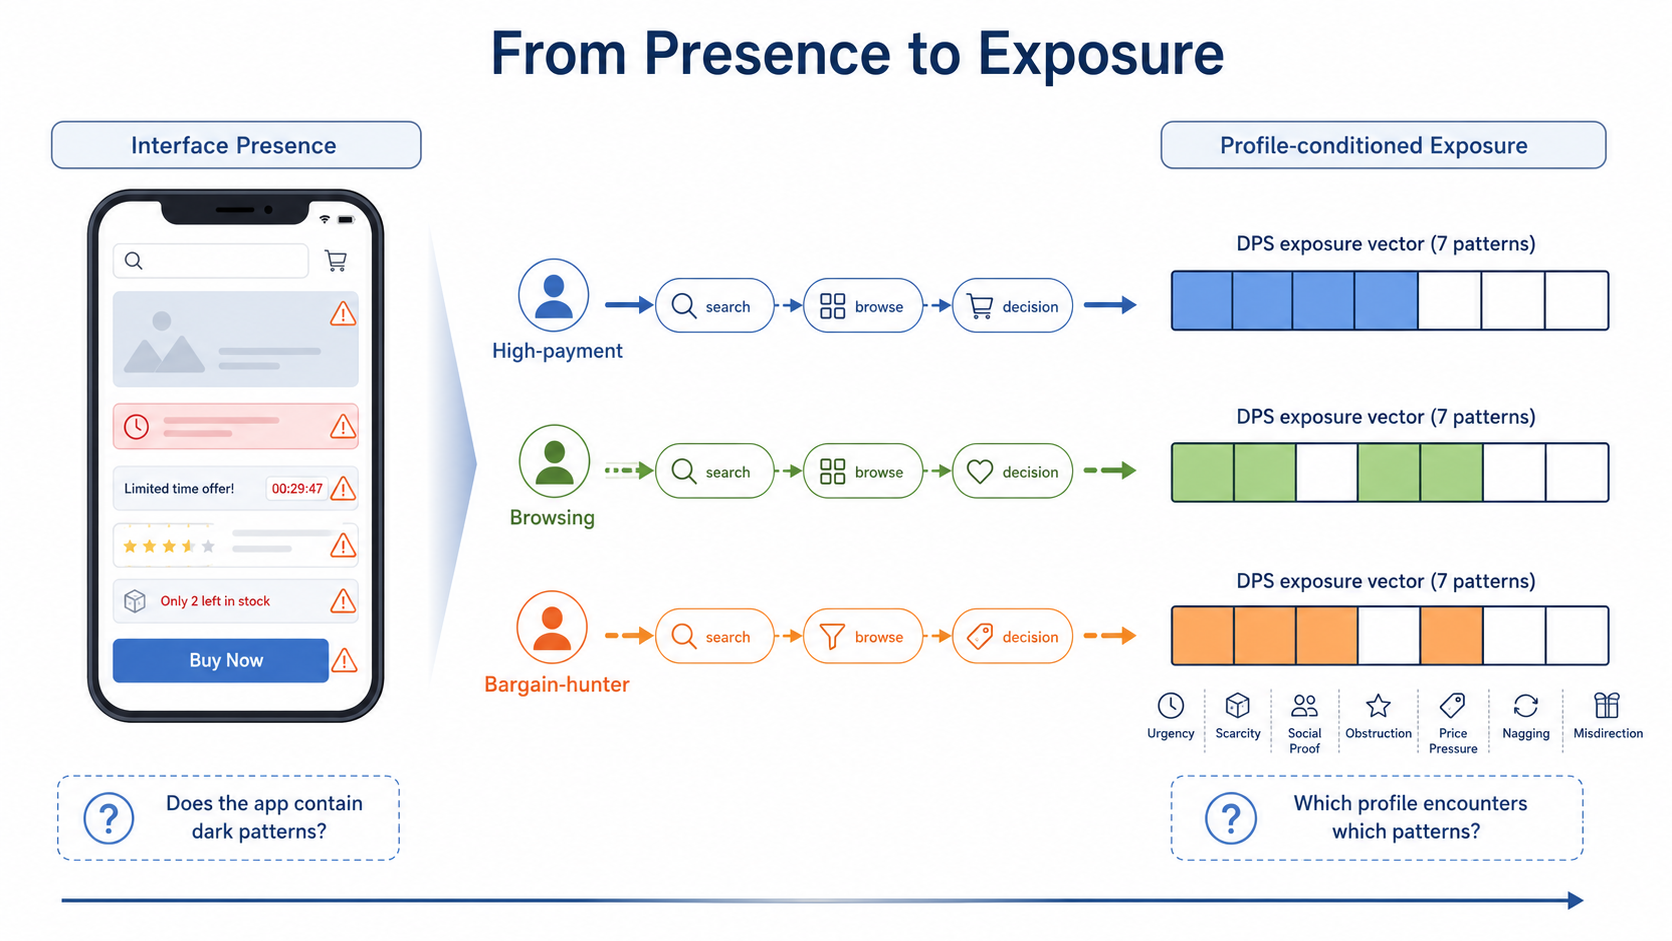
\includegraphics[width=0.95\linewidth]{figures/pictures/presence_to_exposure.png}
    \caption{From Dark Pattern Presence to Profile-Conditioned Exposure.}
    \label{fig:presence-to-exposure}
\end{figure}

\section{Research Questions}

Based on the above motivation, this report investigates personalized dark pattern exposure in mobile applications through a profile-aware auditing framework. The study is organized around four research questions.

\begin{enumerate}
\item \textbf{RQ1: Do different user profiles experience different dark pattern exposure during mobile app interactions?}
This question examines whether controlled profiles produce different observed exposure patterns when interacting with the same set of applications. The focus is not simply on whether an app contains dark patterns, but on whether exposure varies across profile-conditioned interaction trajectories.

\item \textbf{RQ2: Can dark pattern exposure be operationalized as a multidimensional annotation vector suitable for comparison?}  
This question concerns measurement design. Instead of assigning only a single binary label to each screenshot, the project annotates each interaction record using a seven-dimensional Dark Pattern Score vector, \(\mathrm{DPS} = [I, F, P, C, S, N, FA]\), where \(I\) denotes Interface Interference, \(F\) denotes Friction, \(P\) denotes Pressure, \(C\) denotes Contextual Deception, \(S\) denotes Sneaking, \(N\) denotes Nagging, and \(FA\) denotes Forced Action.

\item \textbf{RQ3: Do exposure estimates stabilize over repeated interactions?}  
Since dark pattern exposure may vary from step to step, a single screenshot may not provide a reliable basis for comparison. This question evaluates whether running mean exposure estimates gradually stabilize over repeated interactions, supporting the use of fixed-step exploration trajectories.

\item \textbf{RQ4: Can statistical validation show that observed exposure differences exceed random variation?}  
This question asks whether the measured differences across profiles are larger than what would be expected under random profile assignment. The analysis uses permutation tests, q-values, L1 distance, and Cramér’s V to assess statistical significance and practical association.

\end{enumerate}

\section{Contributions}

This report makes five main contributions. First, it proposes a profile-aware auditing framework for measuring dark pattern exposure in mobile applications. Rather than treating dark patterns only as static interface elements, the framework measures them as observed exposure outcomes along controlled interaction trajectories. This allows the analysis to compare \(E(D \mid A)\), the expected exposure vector conditioned on a user profile \(A\).

Second, the report introduces a controlled profile construction method based on interest and behavior distributions. Interests are represented as probability distributions over keywords, while behaviors are represented as probability distributions over interaction actions. This design makes the profiles reproducible and suitable for black-box auditing, while avoiding demographic attributes that are harder to control and may raise additional ethical concerns.

Third, the report operationalizes dark pattern exposure using a seven-dimensional DPS vector. The vector summarizes key mechanisms discussed in prior dark pattern taxonomies, including interface interference, friction, pressure, contextual deception, sneaking, nagging, and forced action \cite{gray2018darkpatterns,mathur2019darkpatterns,mathur2021whatmakesdark}. This multidimensional representation is more informative than a single presence label because it captures the type of manipulative mechanism encountered in each interaction record.

Fourth, the report presents an empirical audit design involving 16 apps, 3 profiles, and 30 interaction steps per profile-app pair, resulting in 1{,}440 interaction records. Since each record is annotated across seven DPS dimensions, the complete dataset contains 10{,}080 DPS labels. The implementation chapter describes the audit pipeline, while Chapter~\ref{sec:experimental-design} summarizes the experimental scale and annotation structure.

Fifth, the report provides evidence that dark pattern auditing should move beyond interface-level detection toward profile-aware differential exposure analysis. The findings suggest that different profiles show different DPS exposure patterns, that exposure estimates gradually stabilize after repeated interactions, and that statistical validation supports the presence of profile-dependent exposure differences. In particular, the high-payment and bargain-hunter profiles are associated with stronger interface interference and pressure-related exposure, while some app categories, such as food-delivery apps, show consistently high forced-action exposure. These findings do not prove intentional targeting by applications. Rather, they indicate that observed dark pattern exposure may depend on the profile-conditioned interaction trajectory. This perspective expands dark pattern research from the question of whether deceptive interfaces exist to the question of who encounters which mechanisms, under what conditions, and with what measurable differences.

\chapter{Related Work}

\section{Dark Pattern Taxonomies}

Dark patterns, also referred to as deceptive user interfaces, have been widely studied as recurring interface strategies that steer, coerce, or deceive users into decisions that they may not otherwise have made. Early work in human-computer interaction frames dark patterns not merely as examples of poor usability, but as ethically problematic design practices that redirect user attention, effort, or interpretation toward outcomes preferred by service providers \cite{gray2018darkpatterns}. This perspective is important because it shifts the discussion from accidental interface inconvenience to systematic manipulation. A confusing button, a hard-to-find cancellation path, or a visually dominant purchase option may appear as an isolated design choice when observed individually. However, when such patterns recur across platforms and are organized into stable categories, they become measurable design phenomena.

Prior taxonomies have identified a range of dark pattern types, including obstruction, interface interference, sneaking, forced action, nagging, scarcity, social proof, hidden costs, and difficult cancellation \cite{gray2018darkpatterns,mathur2019darkpatterns,mathur2021whatmakesdark}. Obstruction refers to designs that make a user’s intended action unnecessarily difficult, such as requiring many steps to cancel a subscription or reject an optional service. Interface interference changes the presentation of choices by visually emphasizing one option while hiding or weakening another. Sneaking occurs when costs, commitments, or consequences are introduced without sufficient salience, often becoming visible only near the end of a transaction. Forced action requires users to complete an unrelated or undesired action before accessing a service, while nagging repeatedly interrupts the user with prompts or requests that are difficult to dismiss. Scarcity and social proof create pressure by suggesting that a product is limited or popular, while hidden costs and difficult cancellation exploit information asymmetry and procedural friction.

These taxonomies are useful for two reasons. First, they provide a vocabulary for describing deceptive interfaces with greater precision. Instead of treating all manipulative designs as a single vague category, taxonomies distinguish between different mechanisms of influence. Second, they show that dark patterns are systematic rather than isolated design mistakes. If multiple platforms use similar mechanisms, then the problem cannot be fully explained by individual design errors. It reflects broader incentives in digital markets, where interfaces are optimized not only for usability but also for conversion, retention, monetization, and data collection. This report builds on this taxonomic tradition, but it does not attempt to reproduce every fine-grained category. Instead, it operationalizes dark pattern exposure using a seven-dimensional DPS vector that captures several recurring mechanisms: Interface Interference, Friction, Pressure, Contextual Deception, Sneaking, Nagging, and Forced Action.

\section{Dark Patterns as Choice Architecture Manipulation}

A second line of work explains dark patterns through the concept of choice architecture. Choice architecture refers to the way options are organized, displayed, sequenced, and made actionable within a decision environment. In digital interfaces, user decisions are rarely made in a neutral space. Buttons have different colors and sizes, options appear in different locations, defaults may already be selected, and some actions require more effort than others. As a result, the interface can shape decision-making even when the formal set of available options remains unchanged \cite{mathur2021whatmakesdark}.

This perspective is especially useful for understanding why dark patterns can be harmful without relying on a narrow definition of deception. A design does not need to contain a false statement in order to manipulate user choice. It may instead alter option visibility, default choices, visual emphasis, information flow, or the relative effort required to accept or reject an option. For example, an application may make the purchase button large and colorful while placing the decline option in small grey text. It may allow users to accept a membership offer with one tap but require several screens to refuse or cancel it. It may reveal fees only after the user has invested time in the transaction. These designs influence user behavior by restructuring the decision environment.

This interpretation directly motivates several DPS dimensions used later in this report. Interface Interference captures cases where visual hierarchy, layout, or salience directs attention toward a particular option. Friction captures asymmetries in effort, especially when rejecting, leaving, or cancelling is made harder than accepting. Pressure captures urgency, scarcity, countdowns, emotional prompts, and similar cues that encourage quick action. Forced Action captures situations in which users must complete an action, such as registration, payment binding, app installation, or permission granting, before they can proceed. In this sense, the DPS vector is not merely a list of labels. It is an attempt to translate the broader theory of choice architecture manipulation into observable annotation dimensions suitable for screenshot-level and interaction-level auditing.

Understanding dark patterns as choice architecture manipulation also helps avoid overclaiming about user intention or platform intent. This report does not assume that every observed design was intentionally created to deceive. Instead, it focuses on observable interface mechanisms and their association with different user profiles. The question is not whether a designer had malicious intent, but whether controlled profiles encounter systematically different forms or levels of manipulative interface exposure.

\section{Large-scale Measurement of Deceptive Interfaces}

Large-scale measurement studies have shown that dark patterns can be empirically observed, classified, and quantified across digital services. Prior work has examined deceptive patterns in online shopping websites, consent interfaces, and other web or app environments, demonstrating that manipulative designs are not limited to anecdotal examples \cite{mathur2019darkpatterns,nouwens2020gdpr,mathur2021whatmakesdark}. These studies are important because they transform dark patterns from a primarily conceptual or normative concern into a measurable empirical object. Once researchers can identify and count dark pattern instances across many interfaces, they can compare prevalence, categorize mechanisms, and discuss platform accountability with stronger evidence.

For example, large-scale studies of shopping interfaces have shown that commercial platforms frequently use designs related to urgency, scarcity, social proof, hidden costs, and obstruction \cite{mathur2019darkpatterns}. Work on consent pop-ups further demonstrates how interface details such as button placement, default settings, and the visibility of opt-out options can affect user choices \cite{nouwens2020gdpr}. Such studies support the view that interface design can systematically influence user autonomy and consent. They also provide methodological inspiration for this report: dark patterns can be annotated, counted, and compared rather than discussed only through individual examples.

However, much of this measurement work focuses on the presence or absence of dark patterns within an interface. In other words, the central question is often whether a website, app, or page contains a dark pattern. This is a necessary foundation, but it does not fully capture the experience of users in personalized and interactive systems. Mobile applications are not static documents. Users move through different screens, search for different keywords, click different items, and trigger different recommendation or monetization flows. Therefore, two users may interact with the same application but encounter different prompts, pop-ups, membership offers, payment pages, or cancellation paths.

This distinction motivates the shift from dark pattern presence to dark pattern exposure. Presence asks whether a dark pattern exists somewhere in the system. Exposure asks whether a particular user profile actually encounters it during interaction. A dark pattern that exists deep inside an application may have little immediate effect if most users never reach it. Conversely, a pattern that repeatedly appears along a common interaction path may strongly shape user experience. Existing measurement work provides the tools for identifying deceptive interfaces, but this report extends the question toward profile-conditioned exposure along interaction trajectories.

\section{Personalization and Algorithm Auditing}

Digital systems increasingly personalize the outputs that users receive. Search results, recommendations, advertisements, rankings, prices, feeds, notifications, and promotional content may vary according to user history, inferred interests, behavior, device context, or account state. Prior research on personalization has shown that different users can receive different outputs even when they interact with the same platform or issue similar queries \cite{hannak2013personalization}. This finding has motivated broader concerns about differential exposure, because personalized systems may shape what users see, what they believe is available, and what actions they are encouraged to take.

Algorithm auditing provides a methodological foundation for studying such systems from the outside. Because platform internals are often inaccessible, researchers commonly use controlled accounts, scripted behaviors, or sock-puppet profiles to observe outputs under different conditions \cite{sandvig2014auditing}. Auditing studies of recommendation systems, search engines, and content platforms have examined whether different profiles receive different rankings, recommendations, advertisements, or problematic content \cite{ribeiro2020auditing,haroon2023youtubeaudit,srba2023youtube}. These works show that profile-based comparison can reveal differences that would remain hidden if researchers only inspected a platform from a single account or a single interaction path.

This report applies the logic of algorithm auditing to deceptive interface exposure. Instead of asking whether different profiles receive different videos, search results, or advertisements, it asks whether they receive different dark pattern exposure during mobile app interaction. This is a natural extension of auditing research because modern applications often combine personalization with interface optimization. A user who frequently searches for discounts may be shown more promotional prompts. A user who repeatedly enters payment pages may encounter more membership offers, countdowns, or checkout-related pressure. A user who mostly browses without purchasing may encounter fewer payment-oriented interventions. These possibilities should be treated carefully as empirical questions rather than assumed outcomes. Nevertheless, prior auditing research motivates the hypothesis that dark pattern exposure may also be profile-dependent.

The connection between personalization and dark patterns is especially important for social network security and privacy. If manipulative interfaces are personalized, then their impact may not be evenly distributed across users. Some profiles may be more frequently exposed to pressure, forced action, or obstructive flows than others. Ignoring this possibility may obscure how certain behavioral groups are disproportionately steered toward monetization, data disclosure, or continued engagement. Therefore, a profile-aware audit does not replace traditional dark pattern detection. It complements it by asking who encounters which patterns, under what interaction conditions, and with what degree of consistency.

\section{User Modeling for Controlled Audits}

User modeling research commonly represents users through interests, behaviors, and attributes \cite{eke2019userprofiling,piao2018interests,purificato2024usermodeling}. Interests describe what users like or seek, such as product categories, topics, content genres, or keywords. Behaviors describe how users interact, including searching, browsing, clicking, liking, following, watching, staying, dismissing, or entering decision pages. Attributes describe who users are, such as demographic or relatively stable personal characteristics. In real-world personalization systems, these dimensions may be combined to infer preferences and predict future actions.

For controlled audits, however, the goal is not to reconstruct real users in full detail. The goal is to create reproducible profiles that differ along selected dimensions while minimizing uncontrolled variation. This report therefore models user profiles through interests and behaviors, while excluding demographic attributes. Interests are operationalized as probability distributions over keywords. For example, a high-payment shopping profile can be associated with higher probability for high-value product keywords, while a bargain-hunter profile can be associated with discount-related keywords. This design is conceptually related to probabilistic interest modeling, where latent preferences are represented through observable topics, words, or behavioral traces \cite{blei2003lda,piao2018interests}. The report does not claim to infer real user interests through a trained model. Rather, it uses manually specified keyword distributions to create controlled and repeatable audit conditions.

Behaviors are modeled as probability distributions over interaction actions. This abstraction is also consistent with prior work in user behavior modeling and recommendation systems, where clicks, browsing, searches, and sequential actions are treated as behavioral signals \cite{chapelle2009clickmodel,zhou2018din,li2019mind}. In this project, behavior modeling is simplified for auditability. Each controlled profile has an action distribution that determines how often it searches, browses, visits decision interfaces, or performs other interaction steps. The purpose is not to simulate the complete complexity of real mobile users, but to create distinct and interpretable interaction trajectories.

The exclusion of demographic attributes is a deliberate design choice. Demographic features are difficult to control reliably in black-box app audits, especially when platforms may infer them through indirect signals rather than explicit profile fields. They may also raise ethical concerns, particularly if the audit creates or manipulates sensitive identities. By focusing on interests and behaviors, this project studies differential exposure through controllable and reproducible profile dimensions. This choice does not imply that demographic differences are unimportant. Rather, it reflects a course-project scope and an ethical preference for avoiding sensitive attributes while still examining profile-conditioned exposure.

\section{Research Gap}

The literature reviewed above suggests three important conclusions. First, dark pattern research has developed rich taxonomies and measurement methods for identifying deceptive interfaces \cite{gray2018darkpatterns,mathur2019darkpatterns,mathur2021whatmakesdark,nouwens2020gdpr}. These works show that dark patterns are systematic, classifiable, and empirically measurable. Second, algorithm auditing research has demonstrated that digital platforms can produce different outputs for different controlled profiles, especially in personalized search, recommendation, advertising, and content-ranking environments \cite{sandvig2014auditing,hannak2013personalization,ribeiro2020auditing}. Third, user modeling research provides practical abstractions for constructing profiles through interests and behaviors, which can be adapted for controlled audit experiments \cite{eke2019userprofiling,purificato2024usermodeling}.

However, these lines of work are rarely connected directly. Existing dark pattern studies often ask whether a deceptive pattern exists in an interface, but they do not always ask whether different users are exposed to different patterns through different interaction paths. Algorithm auditing studies examine differential outputs across profiles, but they usually focus on search results, recommendations, advertisements, or content exposure rather than deceptive interface mechanisms. User modeling studies provide ways to represent users, but they are not usually used to measure profile-dependent dark pattern exposure.

This report addresses that gap by proposing a profile-aware auditing framework for mobile applications. The framework treats dark pattern exposure as a profile-conditioned outcome rather than a static property of an app. It constructs controlled profiles using interests and behaviors, generates interaction trajectories, annotates each interaction record using the DPS vector, and estimates exposure as \(E(D \mid A)\). By comparing exposure estimates across profiles, the framework examines whether dark pattern exposure is associated with profile differences. This approach does not claim to reveal the internal personalization logic of mobile applications, nor does it establish direct causal intent. Instead, it provides an empirical method for observing and comparing the interface exposure experienced by controlled profiles.

The next chapter builds on this related work by defining the conceptual framework of profile-aware dark pattern auditing. It formalizes user profiles, interaction trajectories, DPS annotation, and profile-conditioned exposure estimation, thereby translating the research gap identified here into an operational audit design.

\chapter{Conceptual Framework}
\label{sec:conceptual-framework}

\begin{figure}[htbp]
    \centering
    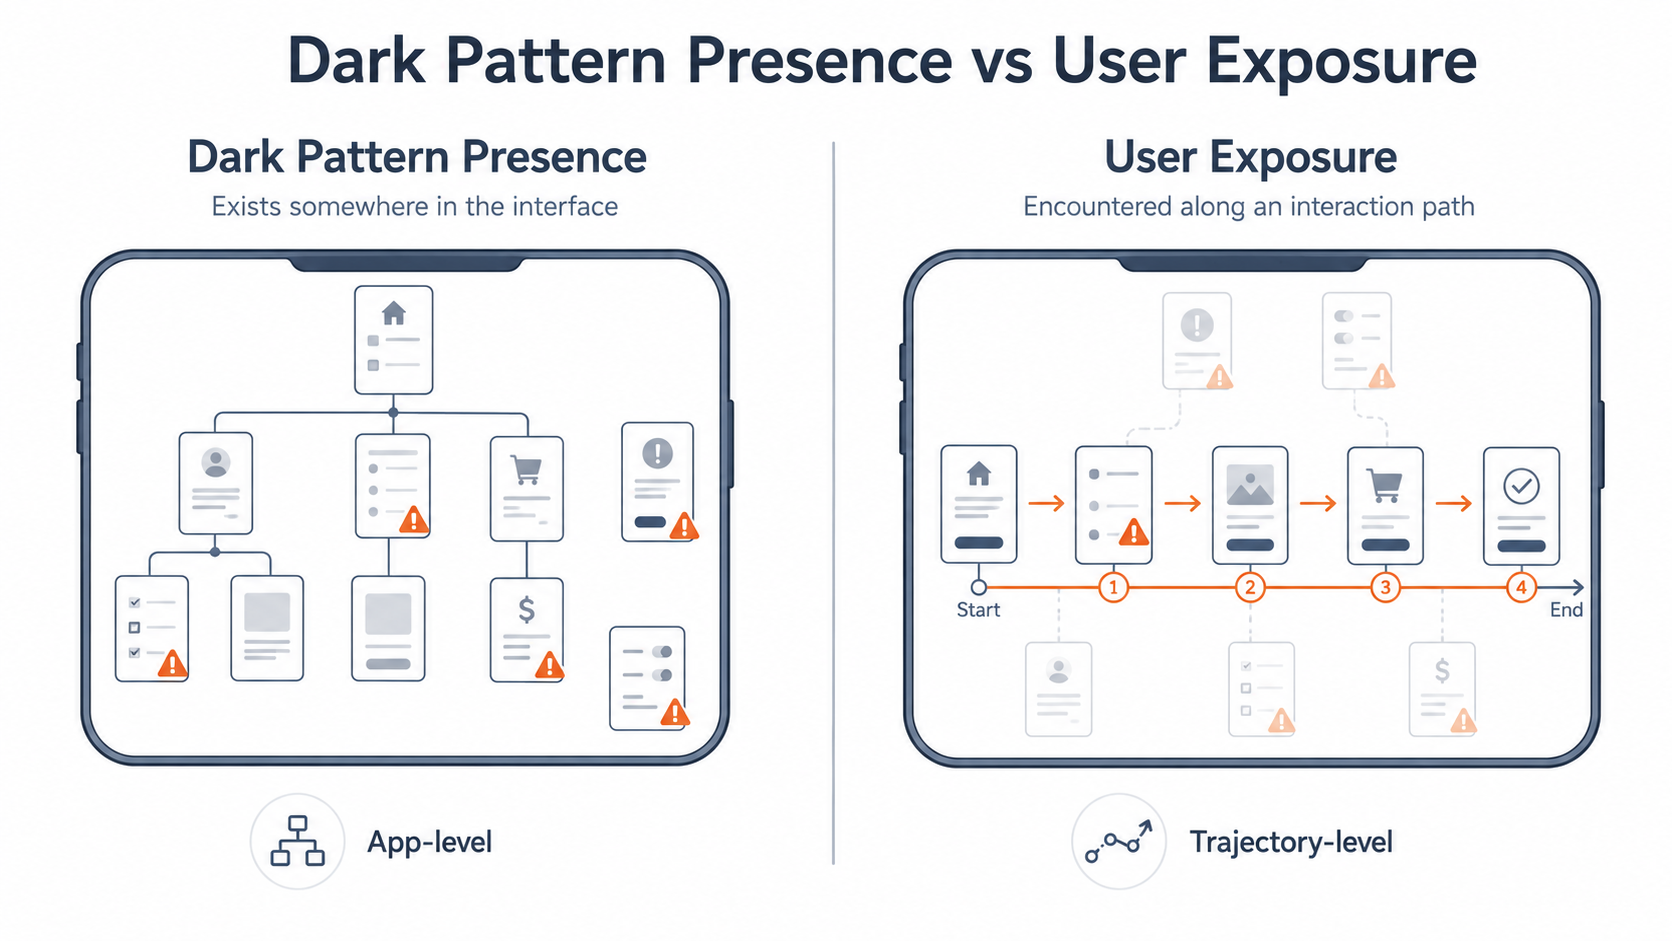
\includegraphics[width=0.95\linewidth]{figures/pictures/presence_vs_exposure.png}
    \caption{Presence vs. Exposure}
    \label{fig:presence_vs_exposure}
\end{figure}


\section{Interface Presence vs. User Exposure}
\label{subsec:presence-exposure}

A central conceptual distinction in this project is the difference between the \emph{presence} of a dark pattern and a user's \emph{exposure} to that dark pattern. Existing studies on deceptive user interfaces have made substantial progress in identifying, categorizing, and measuring dark patterns in websites, mobile applications, and consent interfaces \cite{gray2018darkpatterns,mathur2019darkpatterns,mathur2021whatmakesdark}. In these studies, a dark pattern is often treated as an interface element, design strategy, or choice architecture mechanism that exists somewhere in a digital system. Under this view, a dark pattern is considered present if an application contains, for example, a misleading button, a difficult cancellation path, a countdown timer, a hidden charge, a nagging pop-up, or a forced registration requirement.

However, interface presence alone does not fully describe what users actually experience. A dark pattern may exist in an application but may not be encountered by every user. Some deceptive interface mechanisms appear only after a user searches for a certain keyword, opens a recommended item, enters a payment page, clicks a promotion, or attempts to reject an offer. Others may appear only in specific task flows, such as membership subscription, coupon redemption, food ordering, or checkout confirmation. Therefore, an application-level statement such as ``this app contains a dark pattern'' is informative but incomplete. It indicates that a problematic interface mechanism exists, but it does not indicate whether a particular user profile is likely to encounter it during interaction.

This report therefore shifts the unit of analysis from \emph{dark pattern presence} to \emph{dark pattern exposure}. Exposure refers to the event in which a user actually reaches and observes a dark pattern during an interaction process. In this sense, exposure is conditional on user behavior, search keywords, interface transitions, and the application's response to those actions. This distinction is especially important in mobile applications, where interfaces are dynamic, task-oriented, and often influenced by recommendation or personalization mechanisms. The same application may expose different users to different screens, not necessarily because of explicit demographic targeting, but because different interests and behaviors guide users into different regions of the interface space.

The concept of \emph{differential exposure} further extends this distinction. Differential exposure occurs when different controlled user profiles encounter different types or levels of dark pattern exposure under comparable experimental conditions. For example, a high-payment shopping profile may more frequently reach checkout pages, membership prompts, and urgency-based promotions, while a low-payment browsing profile may remain closer to feeds, homepage browsing, and general content exploration. If their observed DPS annotations differ systematically, the result suggests that dark pattern exposure is associated with profile-conditioned interaction behavior. Importantly, this does not by itself prove intentional targeting by the platform. Rather, it provides empirical evidence that different profiles may experience different observable exposure patterns.

\section{Interaction Trajectories}
\label{subsec:interaction-trajectories}

To analyze exposure rather than mere presence, this project models mobile app usage as an interaction trajectory. A trajectory records the sequence of actions performed by a controlled profile, the interface states reached after those actions, and the dark pattern annotations assigned to the corresponding screenshots. Before defining the trajectory, we first define a simplified action space:

\begin{equation}
\mathcal{A}
=
\{\mathrm{home}, \mathrm{search}, \mathrm{browse}, \mathrm{decision}\}.
\label{eq:action-space}
\end{equation}

Here, $\mathcal{A}$ denotes the set of possible interaction actions used in the conceptual framework. The action $\mathrm{home}$ represents homepage visits or returning to the main interface, $\mathrm{search}$ represents keyword-based search, $\mathrm{browse}$ represents scrolling or opening ordinary content, and $\mathrm{decision}$ represents entering decision-related interfaces such as checkout, subscription, ordering, or confirmation pages. This four-category abstraction is the conceptual action space used throughout the analysis.

The implementation layer may instantiate these categories with a finer-grained action set, such as:

\begin{itemize}
    \item \texttt{visit\_homepage}
    \item \texttt{search\_keyword}
    \item \texttt{browse\_or\_scroll\_page}
    \item \texttt{click\_recommended\_item}
    \item \texttt{like\_or\_favorite}
    \item \texttt{follow\_account}
    \item \texttt{stay\_on\_content}
    \item \texttt{decision\_interface\_visit}
    \item \texttt{close\_popup}
    \item \texttt{back}
\end{itemize}

These implementation-level actions are mapped back to the four conceptual categories before exposure analysis, so the mathematical definitions below remain unchanged while the operational traces can stay more detailed.

Each controlled user profile is represented by two components:

\begin{equation}
A_i = (C_i, B_i),
\label{eq:profile-definition}
\end{equation}

where $A_i$ denotes the $i$-th user profile, $C_i$ denotes the keyword preference distribution of that profile, and $B_i$ denotes its behavior or action distribution. In other words,

\begin{equation}
C_i : \text{keyword preference distribution},
\label{eq:keyword-distribution-text}
\end{equation}

\begin{equation}
B_i : \text{behavior/action distribution}.
\label{eq:behavior-distribution-text}
\end{equation}

The keyword distribution describes what the profile tends to search for, while the behavior distribution describes how the profile tends to interact with the application. For example, a bargain-hunter profile may assign higher probability to keywords such as discounts, coupons, flash sales, or group-buying, while a high-payment shopping profile may assign higher probability to high-value product keywords. Similarly, the high-payment profile may be more likely to enter decision-related interfaces, whereas the low-payment browsing profile may be more likely to browse or scroll.

The behavior distribution of profile $A_i$ is defined as

\begin{equation}
\pi_{A_i}(a)
=
P(a_t = a \mid A_i),
\qquad a \in \mathcal{A}.
\label{eq:behavior-probability}
\end{equation}

This equation means that $\pi_{A_i}(a)$ is the probability that profile $A_i$ performs action $a$ at interaction step $t$. Since $\pi_{A_i}$ is a probability distribution over the action space, it must satisfy

\begin{equation}
\sum_{a \in \mathcal{A}} \pi_{A_i}(a) = 1.
\label{eq:behavior-normalization}
\end{equation}

Similarly, the keyword preference distribution of profile $A_i$ is defined as

\begin{equation}
\rho_{A_i}(w)
=
P(k_t = w \mid A_i, a_t = \mathrm{search}),
\qquad w \in \mathcal{K}_{A_i}.
\label{eq:keyword-probability}
\end{equation}

Here, $k_t$ denotes the keyword selected at step $t$, $w$ denotes a candidate keyword, and $\mathcal{K}_{A_i}$ denotes the keyword set associated with profile $A_i$. This equation means that when profile $A_i$ performs a search action, the keyword is sampled from its profile-specific keyword distribution. The keyword distribution also satisfies a normalization condition:

\begin{equation}
\sum_{w \in \mathcal{K}_{A_i}} \rho_{A_i}(w) = 1.
\label{eq:keyword-normalization}
\end{equation}

At each interaction step, the action is sampled from the profile-conditioned behavior distribution:

\begin{equation}
a_t \sim \operatorname{Categorical}(\pi_{A_i}).
\label{eq:action-sampling}
\end{equation}

This means that the next action is not chosen arbitrarily, but is generated according to the behavioral tendency of the corresponding profile. If the sampled action is search, then the keyword is sampled from the profile-conditioned keyword distribution:

\begin{equation}
k_t \sim \operatorname{Categorical}(\rho_{A_i})
\qquad
\text{if } a_t = \mathrm{search}.
\label{eq:keyword-sampling}
\end{equation}

These equations provide a simple probabilistic model of profile-conditioned interaction. They do not attempt to learn the full behavior of real users. Instead, they define controlled and reproducible profile behaviors for audit experiments. This is suitable for the purpose of the project because the objective is not to infer real user identities or demographic attributes, but to examine whether different controlled behavioral profiles are associated with different dark pattern exposure.

Based on this action generation process, the interaction trajectory of profile $A_i$ is defined as

\begin{equation}
\tau_{A_i}
=
\big(
(a_1, s_1, d_1),
(a_2, s_2, d_2),
\ldots,
(a_T, s_T, d_T)
\big),
\label{eq:trajectory}
\end{equation}

where $a_t$ is the action performed at step $t$, $s_t$ is the resulting interface state or screenshot, $d_t$ is the DPS annotation assigned to that state, and $T$ is the interaction budget. In this project, $T$ is fixed at 30 steps for each app-profile pair. The trajectory therefore connects three components: the action generated by the profile, the interface state returned by the application, and the dark pattern exposure observed in that state.

The annotation $d_t$ is represented as a seven-dimensional DPS vector:

\begin{equation}
d_t
=
[I_t, F_t, P_t, C_t, S_t, N_t, FA_t],
\label{eq:dps-vector-step}
\end{equation}

where $I_t$ denotes Interface Interference, $F_t$ denotes Friction, $P_t$ denotes Pressure, $C_t$ denotes Contextual Deception, $S_t$ denotes Sneaking, $N_t$ denotes Nagging, and $FA_t$ denotes Forced Action at step $t$. This trajectory-based view is important because dark pattern exposure is often sequential. Friction may appear only when the user attempts to reject or cancel an option. Pressure may appear after the user enters a shopping or payment context. Forced action may appear when the user cannot proceed without logging in, granting permission, or accepting a membership prompt. A single static screenshot may miss these mechanisms, while an interaction trajectory can capture how exposure accumulates across repeated app usage.

\begin{figure}[htbp]
    \centering
    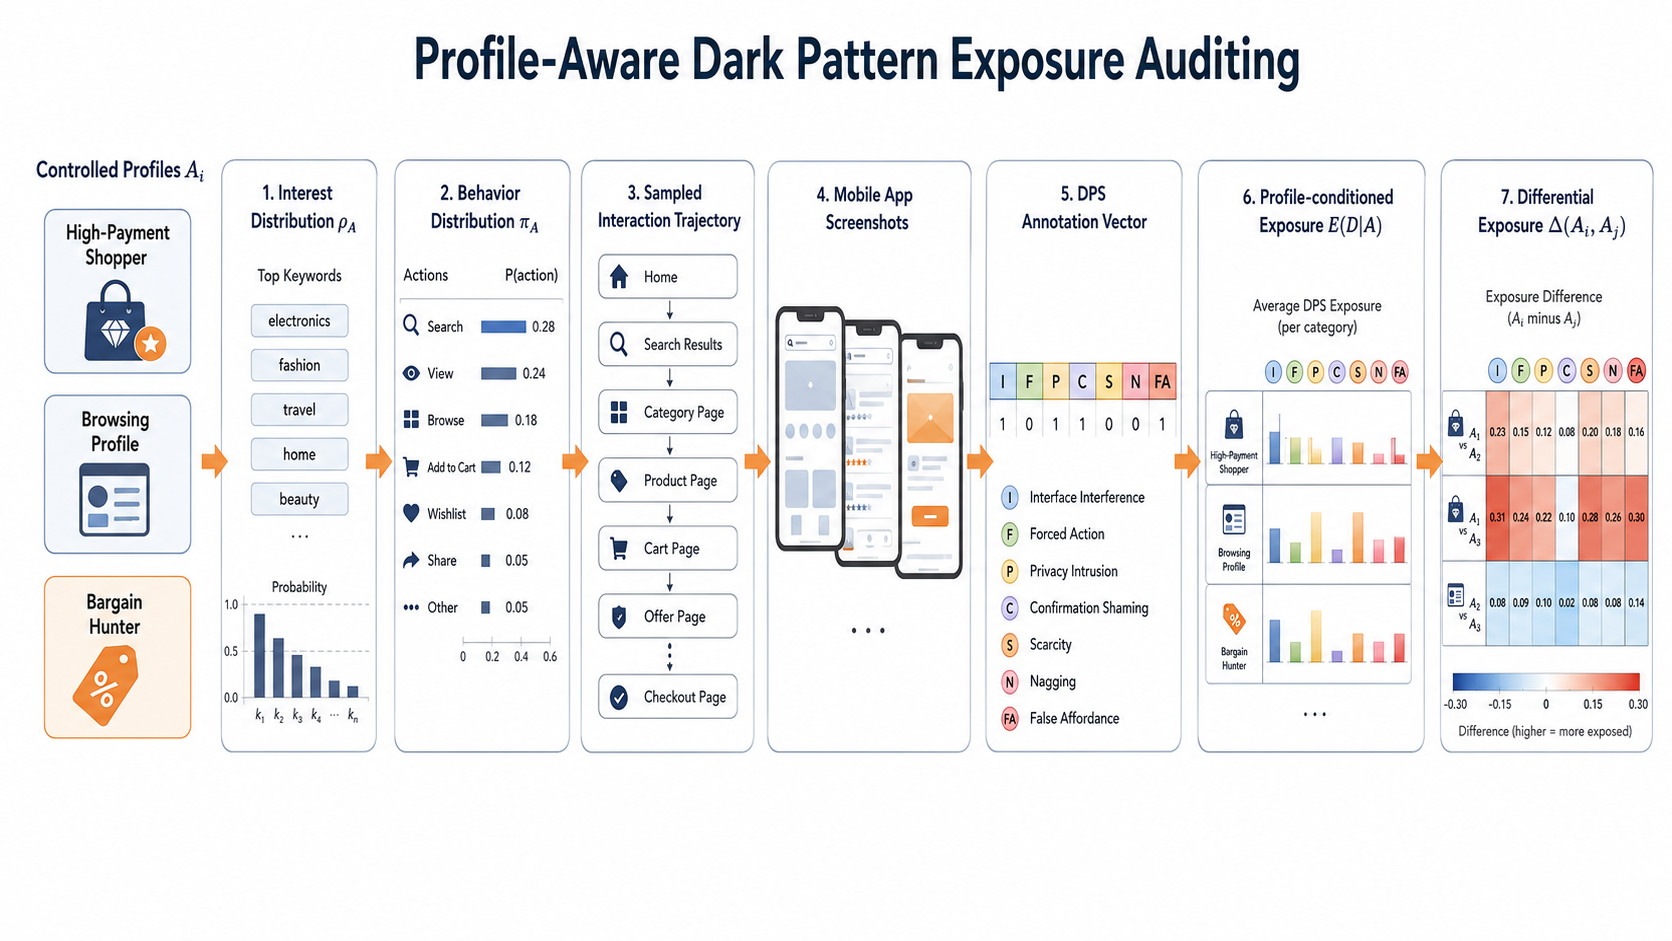
\includegraphics[width=0.95\linewidth]{figures/pictures/core_conceptual_framework.png}
    \caption{Core Conceptual Framework}
    \label{fig:core_conceptual_framework}
\end{figure}

\section{Profile-conditioned Exposure}
\label{subsec:profile-conditioned-exposure}

Based on the trajectory representation, this project defines profile-conditioned dark pattern exposure as

\begin{equation}
E(D \mid A_i),
\label{eq:conditional-exposure}
\end{equation}

where $D$ denotes dark pattern exposure and $A_i$ denotes a controlled user profile. This expression represents the expected or average dark pattern exposure observed under profile $A_i$. Since exposure is annotated using the seven-dimensional DPS vector, the profile-conditioned exposure is also represented as a seven-dimensional vector:

\begin{equation}
E(D \mid A_i)
=
\big[
E(I \mid A_i),
E(F \mid A_i),
E(P \mid A_i),
E(C \mid A_i),
E(S \mid A_i),
E(N \mid A_i),
E(FA \mid A_i)
\big].
\label{eq:conditional-exposure-vector}
\end{equation}

This equation means that the exposure of a profile is not reduced to a single undifferentiated number. Instead, it preserves the type of exposure. Two profiles may have similar overall exposure levels but may encounter different dark pattern mechanisms. For example, one profile may experience more Interface Interference and Pressure, while another may experience more Friction or Forced Action. The vector form makes it possible to compare exposure at the level of individual mechanisms rather than only through total counts.

Empirically, $E(D \mid A_i)$ is estimated by averaging the DPS annotations collected along the interaction trajectories of profile $A_i$. If the profile is tested across multiple applications and multiple steps, the empirical estimate can be written as

\begin{equation}
\widehat{E}(D \mid A_i)
=
\frac{1}{|\mathcal{R}_i|}
\sum_{r \in \mathcal{R}_i} d_r,
\label{eq:empirical-conditional-exposure}
\end{equation}

where $\mathcal{R}_i$ denotes the set of interaction records collected under profile $A_i$, and $d_r$ denotes the DPS vector of record $r$. The hat symbol in $\widehat{E}$ indicates that this is an empirical estimate based on observed data rather than a theoretical expectation known in advance.

This interpretation is important for avoiding causal overclaiming. A higher value of $\widehat{E}(P \mid A_i)$ indicates that profile $A_i$ encountered more pressure-related interface states in the collected audit records. It does not necessarily prove that the application intentionally targeted that profile with pressure mechanisms. The observed pattern may result from recommendation logic, search results, commercial interface design, task flow structure, or the fact that certain profiles enter more decision-sensitive contexts. Therefore, profile-conditioned exposure should be understood as an empirical measure of observed exposure under controlled audit conditions, not as direct evidence of platform intent.

\section{Differential Exposure}
\label{subsec:differential-exposure}

After estimating exposure for each profile, the next step is to compare profiles. Differential exposure between two profiles $A_i$ and $A_j$ is defined as

\begin{equation}
\Delta(A_i, A_j)
=
E(D \mid A_i) - E(D \mid A_j).
\label{eq:differential-exposure}
\end{equation}

This equation defines differential exposure as the difference between two profile-conditioned exposure vectors. Since both $E(D \mid A_i)$ and $E(D \mid A_j)$ are seven-dimensional vectors, $\Delta(A_i, A_j)$ is also a seven-dimensional vector:

\begin{equation}
\Delta(A_i, A_j)
=
[
\Delta I,
\Delta F,
\Delta P,
\Delta C,
\Delta S,
\Delta N,
\Delta FA
].
\label{eq:differential-exposure-vector}
\end{equation}

Each component of this vector corresponds to one DPS dimension. A positive value in $\Delta I$ means that profile $A_i$ encountered more Interface Interference than profile $A_j$ on average. A negative value in $\Delta FA$ means that profile $A_i$ encountered less Forced Action than profile $A_j$ on average. In this way, the difference vector reveals not only whether two profiles differ, but also which dark pattern mechanisms account for the difference.

For example, comparing the high-payment shopping profile with the low-payment browsing profile may indicate whether stronger purchase-oriented behavior is associated with greater exposure to promotional pressure, interface interference, or payment-related forced action. Comparing the bargain-hunter profile with the high-payment shopping profile may show whether discount-oriented behavior is associated with urgency messages, coupon prompts, or membership restrictions. These comparisons move beyond the question of whether an application contains dark patterns and instead ask which profile encounters which mechanisms during interaction.

In addition to the signed difference vector, the overall distance between two exposure vectors can be measured using the $L_1$ distance:

\begin{equation}
L_1(A_i, A_j)
=
\sum_{m=1}^{7}
\left|
E(D_m \mid A_i) - E(D_m \mid A_j)
\right|,
\label{eq:l1-distance}
\end{equation}

where $D_m$ denotes the $m$-th dimension of the DPS vector. This equation sums the absolute differences across all seven DPS dimensions. A larger $L_1$ distance indicates a larger overall separation between the exposure patterns of two profiles, while a smaller value indicates more similar exposure patterns. Unlike the signed vector $\Delta(A_i, A_j)$, the $L_1$ distance does not indicate which profile has more exposure in a particular dimension. Instead, it provides a compact measure of the magnitude of the overall difference.

Together, $\Delta(A_i, A_j)$ and $L_1(A_i, A_j)$ provide complementary views of differential exposure. The difference vector is useful for interpretation because it identifies which dark pattern mechanisms vary across profiles. The $L_1$ distance is useful for summarizing the overall strength of the difference. In the later analysis, these measures can be combined with heatmaps, running mean convergence curves, permutation tests, q-values, and association measures such as Cramér's V to evaluate whether observed profile differences are stable and statistically meaningful.

This conceptual framework establishes the analytical bridge between controlled profile behavior and measurable dark pattern exposure. Rather than treating dark patterns only as static interface artifacts, it treats exposure as a trajectory-based, profile-conditioned, and empirically estimable outcome. The next section builds on this framework by explaining how the controlled profiles are constructed through interests and behaviors while excluding demographic attributes.

\chapter{Profile Construction}

This section describes how controlled user profiles are constructed for the proposed profile-aware auditing framework. In this project, profiles are not treated as informal persona descriptions, but as reproducible experimental objects that can generate observable interaction trajectories. The goal is to examine whether different profile-conditioned interaction patterns are associated with different levels or types of dark pattern exposure in mobile applications.

\section{Design Principles}

The construction of user profiles follows five design principles: controllability, reproducibility, behavioral plausibility, ethical safety, and comparability. These principles are important because the objective of the project is not to infer the true psychological state of real users, but to build controlled profile conditions for auditing mobile applications.

First, profiles should be controllable. A profile must be defined by explicit parameters that can be changed, fixed, or compared across experimental runs. For this reason, the project avoids vague descriptions such as ``a shopping user'' or ``a casual user'' unless they are translated into operational variables. In the framework, a profile is defined through interest distributions and behavior distributions. These distributions determine what keywords are searched and what types of actions are more likely to be performed during exploration. This makes the profile an experimental input rather than a loose narrative label.

Second, profiles should be reproducible. If the same profile is used again under the same experimental configuration, it should produce a similar tendency of interactions, even though individual actions may be sampled probabilistically. Reproducibility is necessary because the audit compares exposure across profiles. If profile behavior were not formally specified, it would be difficult to determine whether observed differences came from the application interface or from inconsistent manual exploration. This principle is consistent with controlled audit methods in which external researchers study black-box platforms through predefined experimental conditions \cite{sandvig2014auditing,hannak2013personalization}.

Third, profiles should be behaviorally plausible. Although the profiles are simplified, they should correspond to recognizable patterns of mobile app use. For example, a high-payment shopping profile should search for high-value goods and enter purchase-related interfaces more frequently than a low-payment browsing profile. A bargain hunter profile should search for discounts, coupons, and flash sales more frequently than the other profiles. The profiles are not intended to perfectly represent real users, but they should be plausible enough to trigger meaningful application responses.

Fourth, profiles should be ethically safe. The project avoids sensitive demographic attributes, such as gender, age, income, ethnicity, or health condition. Instead, it uses interests and behaviors because they are easier to control and less ethically risky in a course-scale audit. This design reduces privacy concerns and avoids constructing profiles that could be interpreted as targeting protected or sensitive groups.

Finally, profiles should be comparable. Since the purpose of the project is to estimate profile-conditioned dark pattern exposure, each profile should be defined using the same formal structure. The profiles differ in probability values and keyword pools, but they share the same modeling framework. This allows exposure estimates such as \(E(D \mid A)\) and pairwise differences such as \(\Delta(A_i,A_j)\) to be interpreted as comparisons between controlled profile conditions.

\section{Formal Definition of User Profiles}

Let \(A_k\) denote the \(k\)-th controlled user profile. In this project, a profile is formally defined as

\[
A_k = (C_k, B_k),
\]

where \(C_k\) is the interest component and \(B_k\) is the behavior component. The interest component describes what content, products, or topics the profile tends to search for. The behavior component describes how the profile tends to interact with the mobile application.

The behavior component is represented as a probability distribution over a predefined action set. Let \(a_t\) denote the action performed at interaction step \(t\). The behavior distribution of profile \(A\) is defined as

\[
\pi_A(a) = P(a_t = a \mid A),
\]

where \(a\) is an action from the action space, such as visiting the homepage, searching a keyword, browsing or scrolling, clicking a recommended item, opening a payment page, closing a popup, or going back. The distribution \(\pi_A(a)\) specifies how likely a profile is to perform each action at a given step.

At the conceptual level, these behaviors are still interpreted through the four categories defined in Chapter~\ref{sec:conceptual-framework}: home, search, browse, and decision. If the implementation uses finer-grained operational actions, those actions are collapsed back into the four conceptual categories before profile-level comparison and exposure analysis.

The interest component is represented as a probability distribution over keywords. Let \(w_t\) denote the keyword selected at step \(t\), when the current action is keyword search. The interest distribution is defined as

\[
\rho_A(w) = P(w_t = w \mid A, a_t = \text{search}),
\]

where \(w\) is a keyword or keyword category in the profile-specific keyword pool. The condition \(a_t = \text{search}\) indicates that keyword sampling only occurs when the sampled action is a search action. In other words, \(\pi_A(a)\) determines whether the profile searches, while \(\rho_A(w)\) determines what the profile searches for.

This separation between behavior and interest is useful because two profiles may share similar action frequencies but differ in search intent, or they may share some keywords but differ in how often they enter decision-related interfaces. For example, a high-payment profile and a bargain hunter profile may both interact with shopping interfaces, but the former emphasizes high-value products while the latter emphasizes promotions and discounts. By separating \(C_k\) and \(B_k\), the framework can represent such differences more clearly.

\section{Interest Modeling}

User interests are not directly observable in mobile applications. A researcher cannot directly observe what a user truly wants, values, or intends to purchase. However, interests can be approximated through observable signals such as search keywords, clicked items, browsed categories, and repeated interactions. User modeling and recommendation research commonly represents latent user interests through observable behavioral traces or probabilistic topic representations \cite{blei2003lda,piao2018interests,zhou2018din}.

In this project, interests are modeled as probability distributions over keyword categories. This design is intentionally simple. Instead of learning user interests from large-scale historical data, the project manually defines keyword pools for each profile. The purpose is not to build a complete recommender-system user model, but to create controlled and reproducible audit conditions.

Search keywords are important because they may influence many downstream interfaces in mobile applications. A search for high-value electronics may lead to premium product pages, installment payment options, membership prompts, or warranty-related recommendations. A search for daily necessities may lead to ordinary browsing results and fewer high-pressure purchase prompts. A search for coupons or flash sales may lead to countdowns, scarcity messages, limited-time offers, or membership reward pages. Therefore, even when the application is treated as a black box, keyword choice provides a practical way to condition the interaction trajectory.

The three profiles use different keyword tendencies. The high-payment shopping profile emphasizes keyword categories such as high-value electronics, premium goods, branded products, and relatively expensive shopping items. The low-payment browsing profile emphasizes daily necessities, casual browsing keywords, ordinary products, snacks, home supplies, and other lower-intent search terms. The bargain hunter profile emphasizes discounts, coupons, flash sales, group-buy offers, membership rewards, and other promotion-sensitive keywords.

These keyword categories are not intended to exhaust all possible user interests. Rather, they provide controlled signals that can be repeatedly used across applications. They also make the audit easier to inspect: when a profile receives stronger pressure-related exposure, the researcher can examine whether such exposure appears after high-value searches, promotion-related searches, or decision-interface visits.

\section{Behavior Modeling}

The behavior component models how a profile interacts with mobile applications. In real systems, user behavior is complex, sequential, and context-dependent. A real user may change intention after seeing a product, abandon a page because of price, or return to the homepage after encountering a popup. However, fully modeling real user behavior is beyond the scope of this course project. Instead, the framework simplifies behavior as a probability distribution over actions.

This simplification follows the logic of probabilistic user interaction models, where user actions such as clicks, browsing, and transitions can be represented as stochastic events \cite{chapelle2009clickmodel}. The purpose is not to claim that users behave according to fixed probabilities in reality. Rather, the purpose is to create controlled behavioral tendencies that can be reproduced across profiles and applications.

The action space includes common mobile app operations, such as homepage visit, keyword search, browsing or scrolling, clicking a recommended item, opening a decision interface, opening a payment or membership page, closing a popup, and going back. These actions cover both low-intent exploration and high-intent decision paths. In particular, decision-interface actions are important because many dark patterns appear near moments of user decision, such as checkout pages, membership subscription pages, coupon redemption pages, or confirmation dialogs. In the implementation, these operations may be represented by more specific action names, but the analysis still collapses them into the four conceptual categories above.

Table~\ref{tab:profile-behavior-probabilities} summarizes the behavior probability examples used by the three profiles. These probabilities are manually assigned according to profile assumptions. They should be interpreted as controlled experimental settings rather than empirical estimates of real-world user populations.

\begin{table}[htbp]
\centering
\caption{Example behavior probability distributions for controlled profiles.}
\label{tab:profile-behavior-probabilities}
\begin{tabular}{lcccc}
\toprule
\textbf{Profile} & \textbf{Homepage Visit} & \textbf{Search Keyword} & \textbf{Browse/Scroll} & \textbf{Decision Interface Visit} \\
\midrule
High-payment shopping & 0.05 & 0.25 & 0.40 & 0.30 \\
Low-payment browsing & 0.15 & 0.15 & 0.60 & 0.10 \\
Bargain hunter & 0.10 & 0.35 & 0.35 & 0.20 \\
\bottomrule
\end{tabular}
\end{table}

The behavior distribution makes the profiles comparable. All profiles are defined over the same abstract action categories, but the probability mass is assigned differently. Therefore, if exposure differs across profiles, the difference can be analyzed in relation to controlled differences in search frequency, browsing frequency, and decision-interface frequency.

\section{High-payment Shopping Profile}

The high-payment shopping profile represents a user condition with stronger commercial intent. This profile frequently searches for high-value goods, browses product details, and enters purchase-related, checkout-related, membership-related, or decision-related interfaces. Its example behavior distribution assigns probability \(0.05\) to homepage visit, \(0.25\) to keyword search, \(0.40\) to browsing or scrolling, and \(0.30\) to decision interface visit.

This profile is designed to test whether mobile applications expose commercially active users to stronger dark pattern mechanisms. Since the profile more often approaches decision points, it may encounter more prompts related to purchase completion, membership enrollment, limited-time discounts, warranty add-ons, or payment confirmation. Such contexts may be associated with interface interference, pressure, sneaking, or forced action. For example, the application may highlight one payment option more strongly than another, make the refusal path less visible, insert additional add-on services, or require the user to pass through membership prompts before continuing.

It is important not to overclaim that the profile causes these dark patterns to appear. The audit only observes whether this controlled interaction pattern is associated with a higher level of exposure. If the high-payment profile receives stronger DPS values in certain dimensions, the result suggests that commercially intensive trajectories may be more exposed to manipulative decision interfaces. The interpretation remains observational because the internal personalization mechanisms of the applications are not directly accessible.

\section{Low-payment Browsing Profile}

The low-payment browsing profile represents a user condition with weak purchasing intent. This profile mainly browses and scrolls, performs fewer decision-related actions, and rarely enters payment or membership interfaces. Its example behavior distribution assigns probability \(0.15\) to homepage visit, \(0.15\) to keyword search, \(0.60\) to browsing or scrolling, and \(0.10\) to decision interface visit.

This profile is useful as a baseline because it captures a relatively low-intent mode of app interaction. Many users open mobile applications without a clear purchase goal. They may browse feeds, inspect ordinary content, compare products casually, or leave before reaching checkout. By assigning more probability to browsing and less probability to decision-interface visits, the profile provides a contrast against more commercially intensive profiles.

The baseline role of this profile does not imply that it should receive no dark pattern exposure. Dark patterns may still appear on homepages, recommendation feeds, login prompts, popups, or content pages. However, compared with profiles that frequently search for high-value goods or promotion-related offers, the low-payment browsing profile is expected to encounter fewer decision-stage prompts. Therefore, differences between this profile and the other two profiles help distinguish general app-level exposure from exposure associated with stronger commercial or promotional intent.

\section{Bargain Hunter Profile}

The bargain hunter profile represents a discount-sensitive user condition. This profile frequently searches for discounts, coupons, flash sales, group-buy offers, membership rewards, and other promotion-related opportunities. Its example behavior distribution assigns probability \(0.10\) to homepage visit, \(0.35\) to keyword search, \(0.35\) to browsing or scrolling, and \(0.20\) to decision interface visit.

This profile is designed to examine whether promotion-oriented trajectories are associated with stronger pressure-related exposure. Discount-sensitive interactions may lead users to pages that emphasize urgency, scarcity, or conditional benefits. For example, applications may display countdown timers, limited-stock messages, social proof, membership-only prices, reward expiration notices, or bundled offers. These interface elements are not necessarily dark patterns in every context, but they may become problematic when they pressure users, obscure alternatives, or make refusal unnecessarily difficult.

Compared with the high-payment profile, the bargain hunter profile has a stronger search tendency but a lower decision-interface probability. This reflects a user who actively looks for promotional opportunities but may still compare options before making a decision. Compared with the low-payment browsing profile, it is more commercially directed and more likely to interact with promotional mechanisms. Therefore, it provides a useful middle condition between casual browsing and high-intent purchasing.

If this profile shows higher exposure in pressure, interface interference, or contextual deception, the finding would suggest that promotional search behavior may be associated with more manipulative or attention-capturing interface designs. However, as with the other profiles, the result should be interpreted as profile-conditioned association rather than proof of causal targeting.

\section{Excluding Demographic Attributes}

The framework intentionally excludes demographic attributes from profile construction. Although user profiling research often discusses attributes such as age, gender, location, income, or other personal characteristics, these attributes are not used in this project. The decision is motivated by reproducibility, controllability, privacy, and ethical concerns.

From a reproducibility perspective, demographic attributes are difficult to operationalize consistently in a course-scale audit. Many mobile applications may not explicitly request demographic information, while others may infer it through opaque mechanisms. If the audit included demographic attributes, it would be unclear whether the application actually received, inferred, or used those attributes. This would make profile construction less reliable.

From a controllability perspective, interests and behaviors are easier to manipulate experimentally. A researcher can control which keywords are searched, which pages are opened, and how frequently decision interfaces are visited. In contrast, demographic attributes are often either unavailable, unverifiable, or entangled with account history and platform inference. Using them would introduce additional uncertainty into the experiment.

From a privacy and ethics perspective, excluding demographic attributes reduces the risk of constructing sensitive or potentially discriminatory user categories. The project aims to audit differential exposure without simulating protected groups or making claims about real demographic populations. This is especially important because dark pattern exposure may relate to vulnerability, manipulation, and unequal treatment. A course-scale project should avoid unnecessary collection or simulation of sensitive identity attributes.

Using interests and behaviors is sufficient for the objective of this audit. The project does not attempt to determine whether platforms discriminate against demographic groups. Instead, it asks a narrower and more controllable question: whether different interest-behavior profiles encounter different dark pattern exposure during mobile app interaction. This design keeps the audit experimentally manageable, ethically safer, and more reproducible while still addressing the central concern of profile-dependent exposure.

\chapter{DPS Annotation Framework}

\section{Motivation for DPS}

A central methodological challenge in this project is how to convert mobile application screenshots into analyzable evidence of dark pattern exposure. Prior research on dark patterns has developed conceptually rich taxonomies that distinguish many types of deceptive or manipulative interface designs, including nagging, obstruction, sneaking, interface interference, forced action, scarcity messages, social proof, hidden costs, preselection, and other forms of choice manipulation \cite{gray2018darkpatterns,mathur2019darkpatterns,mathur2021whatmakesdark}. These taxonomies are valuable because they reveal the diversity of dark pattern mechanisms and provide a theoretical vocabulary for discussing how interfaces may influence user decisions. However, their richness also creates a practical difficulty for screenshot-level annotation. When an annotator observes a single screen in a mobile app, it is often difficult to decide which fine-grained category best describes the interface, especially when several mechanisms appear simultaneously.

For example, a membership popup may visually emphasize an ``Activate Now'' button, hide the close icon, and use wording that suggests the offer is urgent. A fine-grained taxonomy might classify these elements separately as visual interference, obstruction, urgency, or misdirection. In practice, however, requiring annotators to choose from many overlapping labels can reduce consistency and make large-scale annotation difficult. Since this project collects 1,440 interaction records and assigns seven labels to each record, producing 10,080 DPS labels in total, the annotation scheme must be compact, reproducible, and easy to apply across different apps and profiles.

The DPS framework is designed to address this need. Instead of reproducing every category from previous taxonomies, it abstracts common dark pattern mechanisms into seven dimensions that can be applied at the screenshot level. This abstraction does not replace prior taxonomies; rather, it operationalizes them for the specific purpose of profile-aware auditing. The goal is not to identify every possible subtype of dark pattern, but to measure whether different controlled user profiles are exposed to different kinds of manipulative interface mechanisms during mobile app interaction. In this sense, DPS serves as a bridge between qualitative dark pattern concepts and quantitative exposure analysis.

This compact representation is also necessary because the project studies exposure as a distributional outcome. Each screenshot is treated as one observation generated under a particular app, profile, and interaction step. To compare exposure across profiles, the project needs a consistent vector representation that can be averaged, compared, and statistically tested. The DPS vector therefore provides the basis for estimating profile-conditioned exposure, computing pairwise exposure differences, drawing heatmaps, plotting running mean convergence curves, and conducting permutation-based validation.

\begin{figure}[htbp]
    \centering
    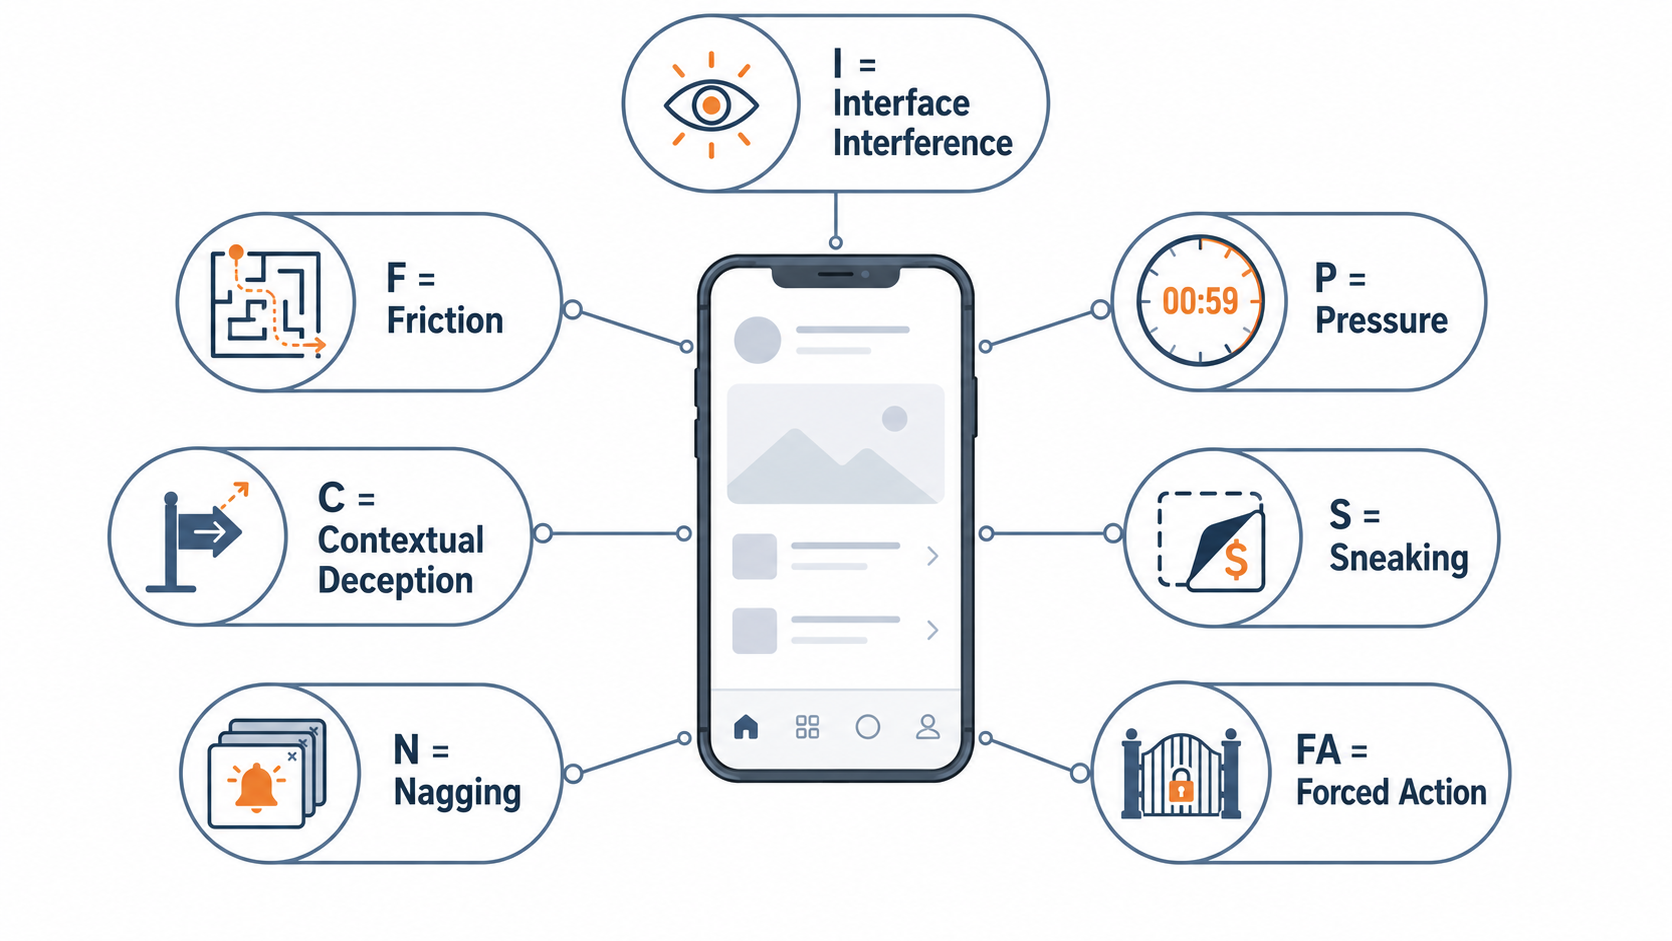
\includegraphics[width=0.95\linewidth]{figures/pictures/seven-dimensional_DPS_vector.png}
    \caption{Seven-Dimensional DPS Vector}
    \label{fig:seven-dimensional-dps-vector}
\end{figure}

\section{DPS Vector Definition}

The project represents dark pattern exposure using a seven-dimensional vector called DPS, defined as follows:

\[
\mathrm{DPS} = [I, F, P, C, S, N, FA],
\]

where \(I\) denotes Interface Interference, \(F\) denotes Friction, \(P\) denotes Pressure, \(C\) denotes Contextual Deception, \(S\) denotes Sneaking, \(N\) denotes Nagging, and \(FA\) denotes Forced Action. Each screenshot collected during the interaction trajectory is converted into one DPS vector. The vector records whether the screen contains observable evidence of each dimension.

This vector-based representation has three advantages.

\begin{itemize}
    \item It allows different dark pattern mechanisms to co-exist in the same screenshot. A screen may contain both pressure and interface interference, or both forced action and nagging.
    \item It avoids forcing annotators to choose a single dominant category when multiple mechanisms are present.
    \item It supports quantitative comparison across profiles. Once every screenshot is represented as a vector, exposure can be aggregated by app, profile, step, or DPS dimension.
\end{itemize}

In the current implementation, each dimension is annotated as a binary label. For a given screenshot, the value of a dimension is 1 if the corresponding mechanism is present and 0 if it is absent. For example, a screenshot with a countdown timer and a visually emphasized purchase button might be annotated as having pressure and interface interference. A screenshot that requires the user to log in before browsing may be annotated as forced action. The following subsections define each DPS dimension and provide practical annotation guidance.

\section{Interface Interference}

Interface Interference refers to visual or layout manipulation that changes how users perceive available options. It occurs when the interface does not present choices in a neutral or balanced way, but instead visually steers attention toward the platform-preferred option. This dimension is closely related to earlier discussions of manipulative choice architecture and interface interference in dark pattern research \cite{gray2018darkpatterns,mathur2021whatmakesdark}.

A typical example is a popup in which the accept button is large, colorful, and centrally placed, while the reject or close option is tiny, gray, or placed in a corner. Another example is a consent or membership interface where the beneficial option for the platform is highlighted with strong contrast, while the user-protective option is visually minimized. Interface interference may also appear when important information is displayed in small gray text, when the close icon is hidden or visually blended into the background, or when misleading color contrast makes one option appear safer, more natural, or more recommended than another.

The key annotation principle is that Interface Interference should be marked when the visual structure of the screen appears to bias perception of choices. It is not necessary to prove that the user was actually deceived. The annotator only needs to judge whether the layout, color, size, placement, or visibility of interface elements gives unequal perceptual weight to different options. For instance, if a shopping app shows a large orange ``Buy Now'' button and places ``Continue Browsing'' in small gray text at the bottom, the screenshot may be labeled as Interface Interference. If all options are presented with comparable visibility and emphasis, this dimension should normally be marked as absent.

\section{Friction}

Friction refers to additional effort imposed on certain user choices, especially rejecting, canceling, opting out, or exiting. It becomes problematic when the effort is asymmetric: one path is easy, immediate, and visually obvious, while the alternative path requires more steps, repeated confirmation, or hidden navigation. This dimension captures the practical difficulty of exercising a choice, rather than the visual appearance of the choice alone.

For example, canceling a membership may require several screens, while renewing the same membership requires only one tap. Rejecting a promotion may require opening a secondary menu, while accepting it is available on the first screen. An exit path may be hidden behind a small icon or placed outside the main interaction flow. In some cases, the user may be redirected repeatedly before refusal is finally allowed. These patterns do not necessarily deceive the user about what is happening, but they make the undesired choice more burdensome.

The annotation should focus on observable interaction burden. If the screenshot clearly indicates that continuing, accepting, or purchasing is easier than refusing, canceling, or exiting, Friction should be marked as present. However, not every multi-step process should be labeled as friction. Some tasks naturally require multiple steps for security or technical reasons, such as confirming a payment or verifying identity. Friction becomes relevant to DPS when the burden appears selectively attached to the user-protective or platform-dispreferred option. Therefore, annotators should ask whether the interface imposes extra effort asymmetrically, rather than simply whether the screen is complex.

\section{Pressure}

Pressure refers to temporal, emotional, scarcity-based, or social cues that push users toward quick decisions. It captures interface elements that create urgency or anxiety, encouraging users to act before they have fully evaluated the choice. This dimension is associated with dark pattern categories such as urgency, scarcity, social proof, and confirmshaming discussed in previous studies of online shopping and deceptive interface design \cite{mathur2019darkpatterns}.

Examples include countdown timers, limited-time offers, labels such as ``only 2 left,'' statements such as ``many people are viewing this,'' and fear-of-missing-out messages. A discount page may show a timer suggesting that the price will disappear soon. A food-delivery app may display a promotion with wording such as ``Order now before the coupon expires.'' A shopping app may state that an item is selling fast or that other users have recently purchased it. These messages may be legitimate in some cases, but from an annotation perspective they still count as pressure when they are used to accelerate the user's decision.

Annotators should mark Pressure as present when the screenshot contains explicit urgency, scarcity, emotional appeal, or social comparison cues. The label does not require determining whether the claim is true or false. For example, the project does not need to verify whether only two items are actually left in stock. The relevant question is whether the interface uses such a cue to influence the user's decision-making context. If a promotion simply states a price or discount without urgency or emotional framing, Pressure should generally be marked as absent.

\section{Contextual Deception}

Contextual Deception refers to a mismatch between what the user reasonably expects in the current interface context and what an action actually does. In this project, \(C\) specifically means Contextual Deception, not merely confusion. A confusing interface may be poorly designed, but it should be labeled as Contextual Deception only when the screen creates a misleading relationship between the apparent meaning of an action and its actual consequence.

For example, a button may appear to close a popup but instead open a subscription page. Ambiguous wording may hide the actual consequence of clicking, such as making a payment, joining a membership program, or enabling automatic renewal. A button placed near a browsing element may cause accidental transition to checkout. A user who intends to view product details may unexpectedly be redirected to a payment or membership interface. In these cases, the deception is contextual because the meaning of the action depends on the surrounding interface situation.

The annotation should consider the user's likely expectation at that moment. If a close-like icon, back-like button, or neutral browsing action leads to a consequence that is inconsistent with its apparent function, Contextual Deception should be marked as present. By contrast, if the consequence is clearly stated and visually aligned with the action, this dimension should be absent even if the user might dislike the result. This distinction is important because the DPS framework aims to capture deceptive context-action mismatches, not all forms of inconvenience or dissatisfaction.

\section{Sneaking}

Sneaking refers to hiding, delaying, or quietly adding information that affects user decisions. It often appears near checkout, subscription, or membership interfaces, where additional costs or commitments may be introduced without being made salient. This dimension is connected to prior dark pattern categories such as hidden costs, sneak into basket, preselection, and default add-ons \cite{gray2018darkpatterns,mathur2019darkpatterns}.

Examples include hidden fees that are revealed only at the final step, preselected paid add-ons, default inclusion of a subscription, or an extra service added near checkout. A shopping app may automatically select shipping insurance. A food-delivery app may add a paid membership trial by default. A travel or ticketing app may reveal service fees only after the user has already invested effort in the booking process. These mechanisms affect decision-making because the user may proceed under an incomplete understanding of cost or commitment.

Annotators should mark Sneaking as present when the screenshot shows evidence that a cost, service, subscription, or commitment has been added, hidden, delayed, or preselected in a way that may not be immediately expected. If the additional item is clearly optional, not preselected, and equally visible, Sneaking should normally be absent. The key question is whether the interface quietly changes the transaction or decision context in favor of the platform.

\section{Nagging}

Nagging refers to repeated interruptions after users dismiss or ignore a request. Unlike Pressure, which focuses on urgency or emotional influence, Nagging focuses on repetition and interruption. It occurs when the application repeatedly asks the user to perform an action, even after the user has already declined or ignored similar prompts.

Common examples include repeated membership popups, repeated notification permission requests, repeated login prompts, and repeated promotional interruptions. A user may close a membership discount popup, only to see a similar popup again after scrolling or opening another page. A mobile app may repeatedly request notification permission each time the user enters the home screen. A browsing session may be interrupted by login prompts even when login is not necessary for the immediate task.

In annotation practice, Nagging is easiest to identify when interaction history is available. A single screenshot may show a popup, but the nagging label depends on whether similar interruptions have appeared repeatedly during the trajectory. Therefore, annotators should use the current screenshot together with the previous interaction records when judging this dimension. If the same type of request appears repeatedly after dismissal or avoidance, Nagging should be marked as present. If a request appears only once and is relevant to the current task, it should generally not be labeled as nagging.

\section{Forced Action}

Forced Action means that the user must perform an additional action before accessing the intended function. It captures situations where the app blocks the user's original goal unless the user completes a platform-required step. This dimension is derived from prior dark pattern taxonomies that identify forced action as a mechanism for extracting registration, consent, permissions, or other commitments from users \cite{gray2018darkpatterns}.

Examples include requiring login before browsing, requiring notification permission before entering the app, requiring phone-number binding before using a feature, requiring acceptance of unrelated terms, or requiring the user to complete an extra task before continuing. Forced Action is especially relevant in mobile apps because many apps combine browsing, shopping, payment, social features, and account systems in a single interface. As a result, users may encounter blocking screens that require them to provide data, accept permissions, or join programs before reaching the intended function.

Annotators should mark Forced Action as present when access to the user's apparent goal is blocked until an additional action is completed. The label should not be used when the requested action is strictly necessary for the function. For example, payment naturally requires payment confirmation, and account recovery naturally requires identity verification. However, if the user simply wants to browse products and is required to log in, bind a phone number, or enable notifications, Forced Action should be marked as present. In the project findings, some app categories, such as food-delivery apps, show consistently high forced-action exposure, suggesting that this dimension is important for understanding how access control and commercial goals interact in mobile interface design.

\section{Annotation Scale}

In the current version of the DPS framework, each dimension is annotated using a binary scale:

\[
d_i \in \{0, 1\},
\]

where \(d_i = 1\) means that the corresponding DPS dimension is present in the screenshot, and \(d_i = 0\) means that it is absent. A complete DPS vector therefore consists of seven binary values. For example, a screenshot may be represented as:

\[
[1, 0, 1, 0, 0, 0, 0],
\]

which indicates that Interface Interference and Pressure are present, while Friction, Contextual Deception, Sneaking, Nagging, and Forced Action are absent.

The binary scale is chosen for consistency and feasibility. Since the experiment involves 16 apps, 3 profiles, and 30 interaction steps per profile-app pair, the annotation workload is already substantial. A binary scheme reduces ambiguity and allows annotators to focus on whether a mechanism is observable. It also supports straightforward aggregation. For each profile \(A\), the project can estimate the expected exposure \(E(D \mid A)\) by averaging DPS labels across records. Pairwise differences between profiles can then be computed as \(\Delta(A_i, A_j)\), and statistical validation can be conducted using permutation tests, q-values, L1 distance, and Cramér's V.

Future work could extend the binary scale to ordinal scores such as 0, 1, and 2, where 0 indicates absence, 1 indicates weak or moderate presence, and 2 indicates strong presence. Such an extension would allow more nuanced measurement of severity. For example, a small countdown label and a full-screen urgent warning might both be labeled as Pressure under the binary scale, while an ordinal scale could distinguish their intensity. However, ordinal scoring also requires stronger annotation guidelines and reliability checks. For the present course project, the binary scale provides a practical balance between expressiveness and consistency.

\begin{figure}[htbp]
    \centering
    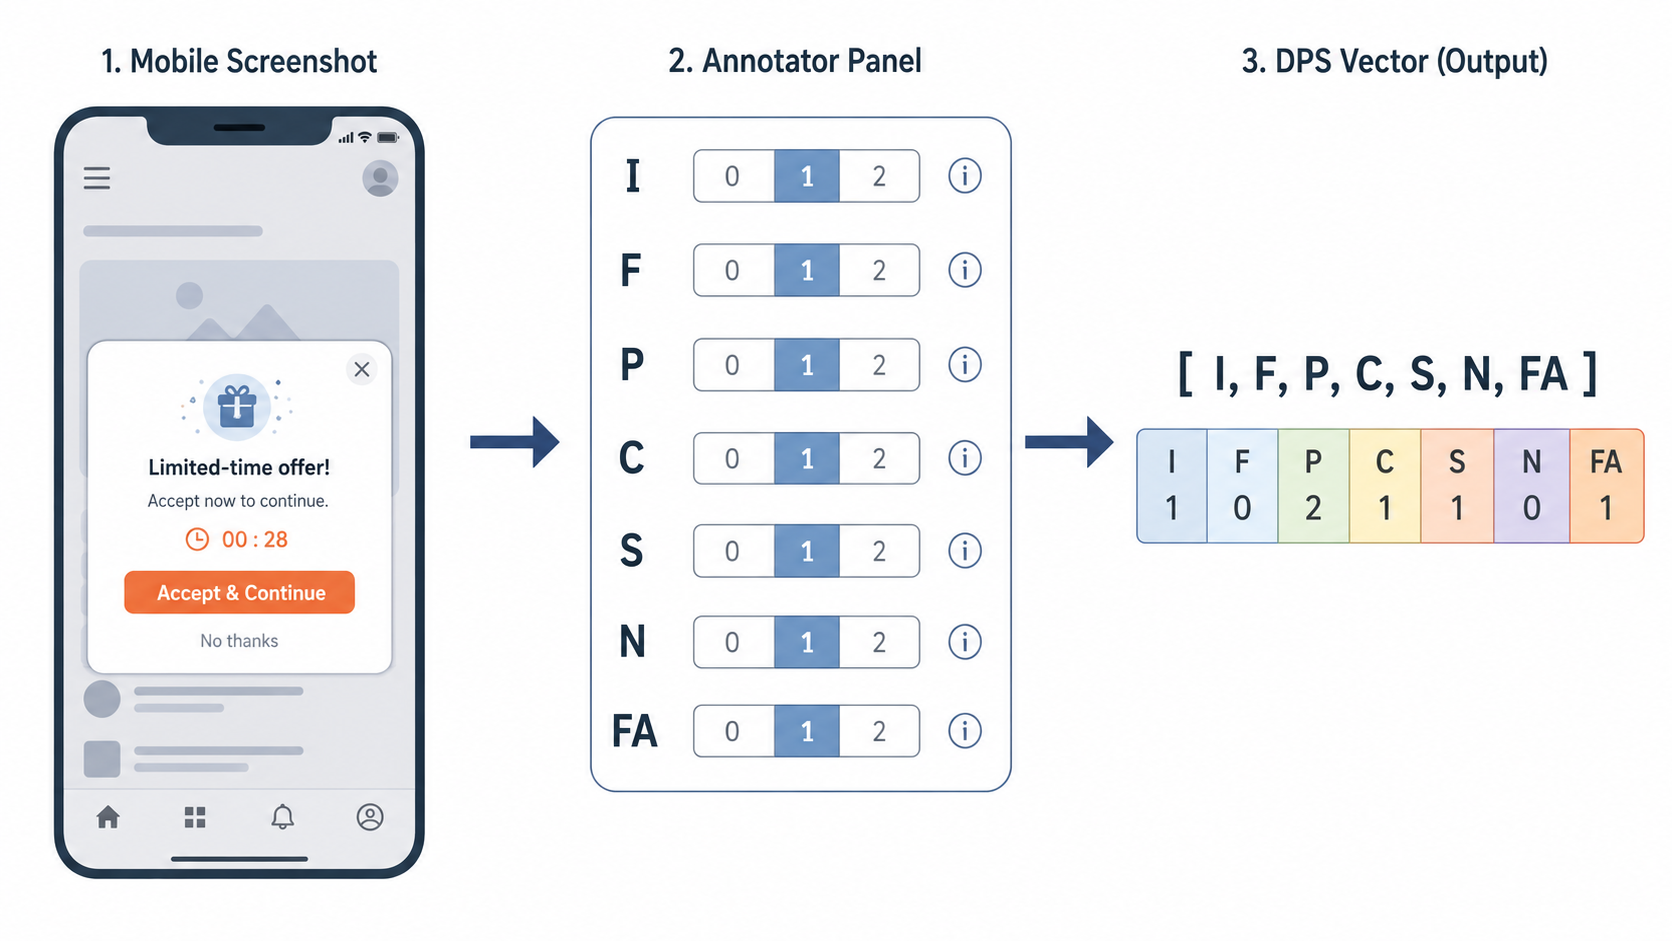
\includegraphics[width=0.95\linewidth]{figures/pictures/from_screenshot_to_DPS_label.png}
    \caption{From Screenshot to DPS Label}
    \label{fig:from-screenshot-to-dps-label}
\end{figure}

\section{Annotation Examples}

Consider a membership popup with a large ``Activate Now'' button and a small close icon in the upper corner. A possible DPS vector is:

\[
[1, 0, 0, 0, 0, 0, 0].
\]

Interface Interference is marked as present because the platform-preferred action is visually emphasized while the exit option is minimized. If the popup appears repeatedly after dismissal, Nagging may also be marked as present, resulting in \([1, 0, 0, 0, 0, 1, 0]\). If the user cannot continue using the app without activating or logging in, Forced Action may also be present. This example shows why DPS annotation should consider both the screenshot and the interaction context.

A second example is a discount page with a countdown timer and wording such as ``limited quantity'' or ``only 2 left.'' A possible vector is:

\[
[0, 0, 1, 0, 0, 0, 0].
\]

Pressure is marked as present because the interface uses temporal urgency and scarcity cues to encourage quick decision-making. If the page also uses a large purchase button and a visually weak refusal option, Interface Interference may be added, producing \([1, 0, 1, 0, 0, 0, 0]\). The annotation does not require proving whether the scarcity claim is accurate. The presence of the pressure cue is sufficient for the label.

A third example is a checkout page with a preselected paid add-on, such as shipping insurance, priority delivery, or a membership trial. A possible vector is:

\[
[0, 0, 0, 0, 1, 0, 0].
\]

Sneaking is marked as present because an additional paid item or service has been quietly included in the transaction. If the add-on is displayed in small gray text or placed in a visually obscure area, Interface Interference may also be present. If removing the add-on requires entering a secondary page or completing several steps, Friction may also be marked. In that case, the vector might become \([1, 1, 0, 0, 1, 0, 0]\). This illustrates how one commercial interface can contain multiple dark pattern mechanisms at the same time.

A fourth example is a page that cannot be accessed unless the user logs in. If the user's intended action is ordinary browsing, a possible vector is:

\[
[0, 0, 0, 0, 0, 0, 1].
\]

Forced Action is marked as present because the app blocks access to the intended function until the user completes an additional action. If the login wall appears repeatedly after the user tries to dismiss it, Nagging may also be present. If the login screen uses a visually dominant one-click authorization button while hiding alternative access paths, Interface Interference may also be present. However, if the user is attempting to perform an action that inherently requires identity verification, such as making a payment or viewing private account information, the forced-action label should be applied more cautiously.

These examples demonstrate that DPS annotation is not merely a mechanical labeling task. It requires attention to the user's immediate goal, the visual presentation of choices, the sequence of previous interactions, and the practical consequences of interface actions. At the same time, the seven-dimensional vector keeps the task sufficiently structured for quantitative analysis. By converting each screenshot into a compact DPS representation, the project can compare dark pattern exposure across controlled profiles without overclaiming about user psychology or platform intent. The resulting framework supports the broader goal of this report: auditing whether different behavioral and interest-based profiles are associated with different levels and types of dark pattern exposure in mobile applications.

\chapter{Differential Exposure Estimation}

\section{Single-step Exposure}

The central objective of this project is to estimate whether different controlled user profiles are associated with different patterns of dark pattern exposure during mobile application interaction. To support this objective, the analysis begins at the level of a single interaction step. Each step in the audit corresponds to one observable interface state produced after a profile-conditioned action is executed. In practice, this state is recorded as a screenshot or a comparable interface observation. The screenshot is then manually annotated using the seven-dimensional Dark Pattern Score vector, abbreviated as DPS.

Formally, the exposure observed at interaction step \(t\) is represented as

\[
D_t = [I_t, F_t, P_t, C_t, S_t, N_t, FA_t],
\]

where \(I_t\) denotes Interface Interference, \(F_t\) denotes Friction, \(P_t\) denotes Pressure, \(C_t\) denotes Contextual Deception, \(S_t\) denotes Sneaking, \(N_t\) denotes Nagging, and \(FA_t\) denotes Forced Action. The vector \(D_t\) therefore represents the dark pattern exposure observed in a single interface state at step \(t\). This formulation follows the broader idea in dark pattern research that deceptive or manipulative interface mechanisms can be operationalized into observable categories rather than treated only as anecdotal examples \cite{gray2018darkpatterns,mathur2019darkpatterns,mathur2021whatmakesdark}.

The single-step vector is intentionally simple. It does not attempt to explain why the interface state appeared, nor does it claim that the user profile caused the application to display that state. Instead, it provides a structured measurement of what was observed after a controlled interaction. A raw component \(D_{t,d}\) is a numeric exposure score, and the binary occurrence variable for that component is \(1[D_{t,d}>0]\). This distinction is important because the project is designed as a profile-aware audit of exposure, not as a causal inference study of platform decision-making. A single vector \(D_t\) should therefore be interpreted as one observed unit of exposure within a longer interaction trajectory.

\section{Profile-level Exposure}

While a single screenshot can reveal whether a particular interface state contains dark pattern mechanisms, it is not sufficient for comparing user profiles. Mobile applications are dynamic systems: pop-ups, recommendations, payment prompts, discounts, and consent interfaces may appear at different moments during interaction. For this reason, the project estimates exposure over repeated interaction steps rather than relying on isolated screenshots.

For a given profile \(A\), the profile-level exposure is defined as the empirical mean of all single-step DPS vectors collected under that profile:

\[
E(D \mid A) = \frac{1}{n_A}\sum_{t=1}^{n_A} D_t.
\]

Here, \(n_A\) is the effective number of audited interaction steps available for profile \(A\), and \(D_t\) is the DPS vector observed at step \(t\). In the project design, each profile is assigned the same target budget, but the archived analysis uses the effective observed length because five trajectories end before the 30-step target. Each profile is audited through repeated controlled interactions, and the resulting vectors are averaged to estimate the typical exposure pattern associated with that profile.

Each dimension of \(E(D \mid A)\) represents either a raw intensity mean or a binary occurrence rate, depending on the analysis. For occurrence-rate analysis, each raw score is first converted to \(1[D_{t,d}>0]\), so a Pressure value of \(0.40\) means that pressure-related mechanisms appeared in approximately 40 percent of the audited interaction states for that profile. For intensity analysis, the raw numeric values are averaged directly, so means can exceed 1 for dimensions scored with counts or ordinal levels. This interpretation makes the exposure vector intuitive while preserving the distinction between whether a mechanism appears and how strongly it appears.

The profile-level estimate is especially useful because the project constructs three controlled user profiles: a high-payment shopping profile, a low-payment browsing profile, and a bargain-hunter profile. These profiles differ in their interest distributions and behavior distributions, but they exclude demographic attributes to improve controllability and reproducibility. Therefore, \(E(D \mid A)\) estimates profile-conditioned exposure under controlled behavioral assumptions rather than exposure for real demographic groups.

\section{Application-level Exposure}

The profile-level estimate summarizes exposure across the audit data for a given profile, but it does not show whether profile differences are consistent within the same application. To address this, the framework also defines application-level exposure:

\[
E(D \mid A, app) = \frac{1}{n_{\mathrm{app},A}}\sum_{t=1}^{n_{\mathrm{app},A}} D_{app,A,t}.
\]

In this expression, \(D_{app,A,t}\) denotes the DPS vector observed in application \(app\), under profile \(A\), at interaction step \(t\). The value \(n_{\mathrm{app},A}\) refers to the effective number of archived interaction steps for that profile within that application. This estimate allows the analysis to compare different profiles while holding the application fixed.

Application-level exposure is important because different mobile applications may implement different interface strategies. A shopping application may emphasize discounts, urgency, and recommendation placement, while a food-delivery application may rely more heavily on login gates, membership prompts, or payment-related decision points. By computing \(E(D \mid A, app)\), the framework can ask whether the high-payment profile encounters more pressure-related exposure than the low-payment profile inside the same application, rather than merely across the full dataset.

Application-level heatmaps make it possible to observe whether profile-conditioned exposure differences are concentrated in particular mechanisms, such as Interface Interference or Pressure. The representative heatmaps in Chapter~\ref{chap:results} use this format to compare exposure across profiles and DPS dimensions. However, the interpretation should remain cautious. A higher value for one profile indicates an observed association between the controlled profile and the exposure pattern in the audit setting; it does not prove the internal logic by which the application generated the interface state.

\section{Category-level Exposure}

In addition to analyzing individual applications, the framework aggregates exposure at the application-category level. Category-level exposure is defined as

\[
E(D \mid A, category),
\]

where \(category\) denotes a group of applications sharing a similar service context, such as shopping, food delivery, entertainment, or social content platforms. In practice, this value can be estimated by averaging the application-level exposure vectors for all applications within the same category, under the same profile.

Category-level exposure is useful because dark pattern mechanisms may be shaped by the functional goals of the application category. For instance, food-delivery applications may require users to log in, choose delivery addresses, enable location access, or enter payment-related information before completing core tasks. As a result, this category may show consistently high Forced Action exposure. By contrast, shopping applications may more frequently display pressure-related elements, such as limited-time offers, promotional rankings, or interface emphasis on high-value items. These patterns are not interpreted as universal properties of the categories, but as observed tendencies in the audited sample.

Category-level exposure estimates help reduce the noise of individual applications and make it easier to identify broader exposure patterns. At the same time, category-level results should not hide application-level variation. Two applications in the same category may still differ substantially in their interface design, business model, and personalization mechanisms.

\section{Pairwise Profile Difference}

To directly compare two profiles, the framework defines a pairwise exposure difference vector:

\[
\Delta(A_i, A_j) = E(D \mid A_i) - E(D \mid A_j).
\]

The resulting vector has the same seven dimensions as the DPS vector. Each component indicates whether profile \(A_i\) encountered more or less of a given dark pattern mechanism than profile \(A_j\). For example, if the Pressure component of \(\Delta(A_i, A_j)\) is positive, then profile \(A_i\) showed higher estimated pressure exposure than profile \(A_j\). If the Forced Action component is close to zero, then the two profiles encountered similar levels of forced-action exposure in the audited data.

This difference vector is more informative than a single aggregate score because dark pattern exposure is multidimensional. Two profiles may have similar overall exposure levels but differ in the mechanisms they encounter. For instance, the high-payment shopping profile and the bargain-hunter profile may both show elevated exposure, but the former may be associated with more high-value product steering while the latter may be associated with more discount urgency or promotional pressure. The pairwise vector preserves this dimensional structure and helps identify which specific DPS mechanisms contribute to the observed profile difference.

\section{Overall Distance Between Profiles}

\begin{figure}[htbp]
    \centering
    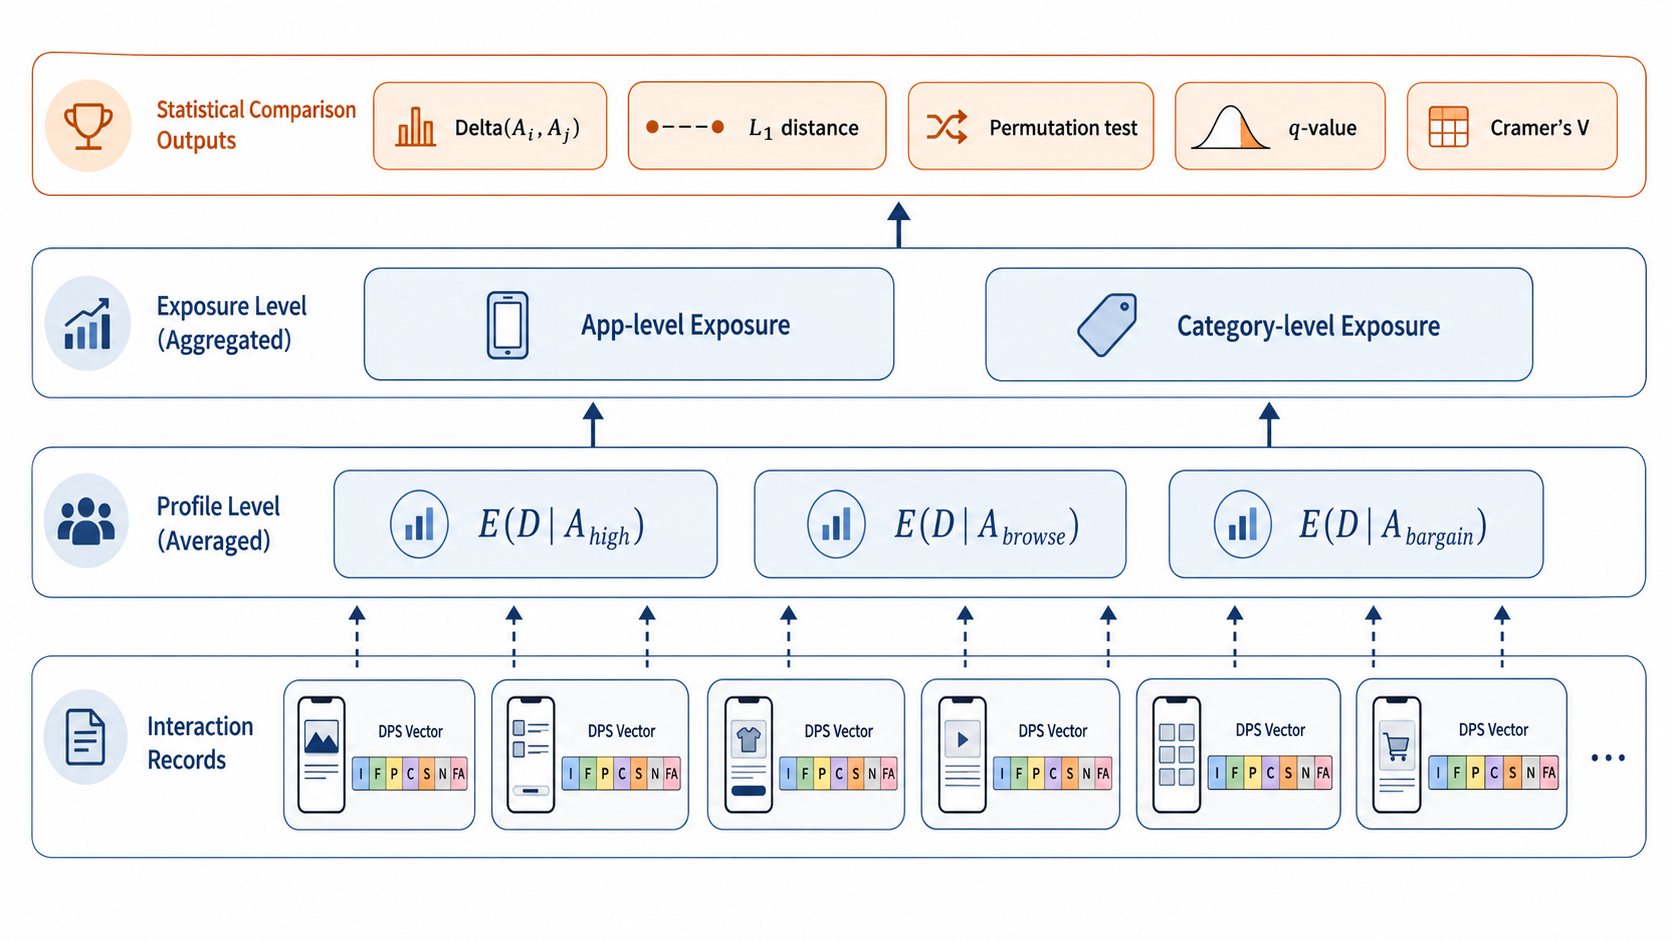
\includegraphics[width=0.95\linewidth]{figures/pictures/exposure_estimation_hierarchy.png}
    \caption{Exposure Estimation Hierarchy}
    \label{fig:exposure-estimation-hierarchy}
\end{figure}

Although the pairwise difference vector is useful for dimension-level interpretation, it is sometimes helpful to summarize the overall magnitude of difference between two profiles. For this purpose, the framework uses the \(L_1\) distance between exposure vectors:

\[
L_1(A_i, A_j) = \sum_{d \in \{I,F,P,C,S,N,FA\}}
\left| E(D_d \mid A_i) - E(D_d \mid A_j) \right|.
\]

Here, \(D_d\) denotes one of the seven DPS dimensions. The \(L_1\) distance sums the absolute exposure differences across all dimensions. A larger value indicates a larger practical difference between the two profile-level exposure patterns, while a smaller value indicates that the profiles encountered more similar dark pattern exposure.

The advantage of \(L_1\) distance is interpretability. It does not require strong distributional assumptions, and it directly reflects how far apart two exposure vectors are across the DPS dimensions. However, it should be read as a descriptive magnitude measure rather than a causal measure. A large \(L_1\) distance suggests that two controlled profiles were associated with meaningfully different exposure patterns in the audit, but it does not identify the precise platform mechanism responsible for that difference.

Figure~\ref{fig:method-l1-distance} illustrates how the \(L_1\) distance is reported across comparison scopes in the empirical analysis. The figure is included here as a representative methodological visualization because it shows how the vector-level exposure difference is converted into a compact magnitude summary.

\begin{figure}[htbp]
    \centering
    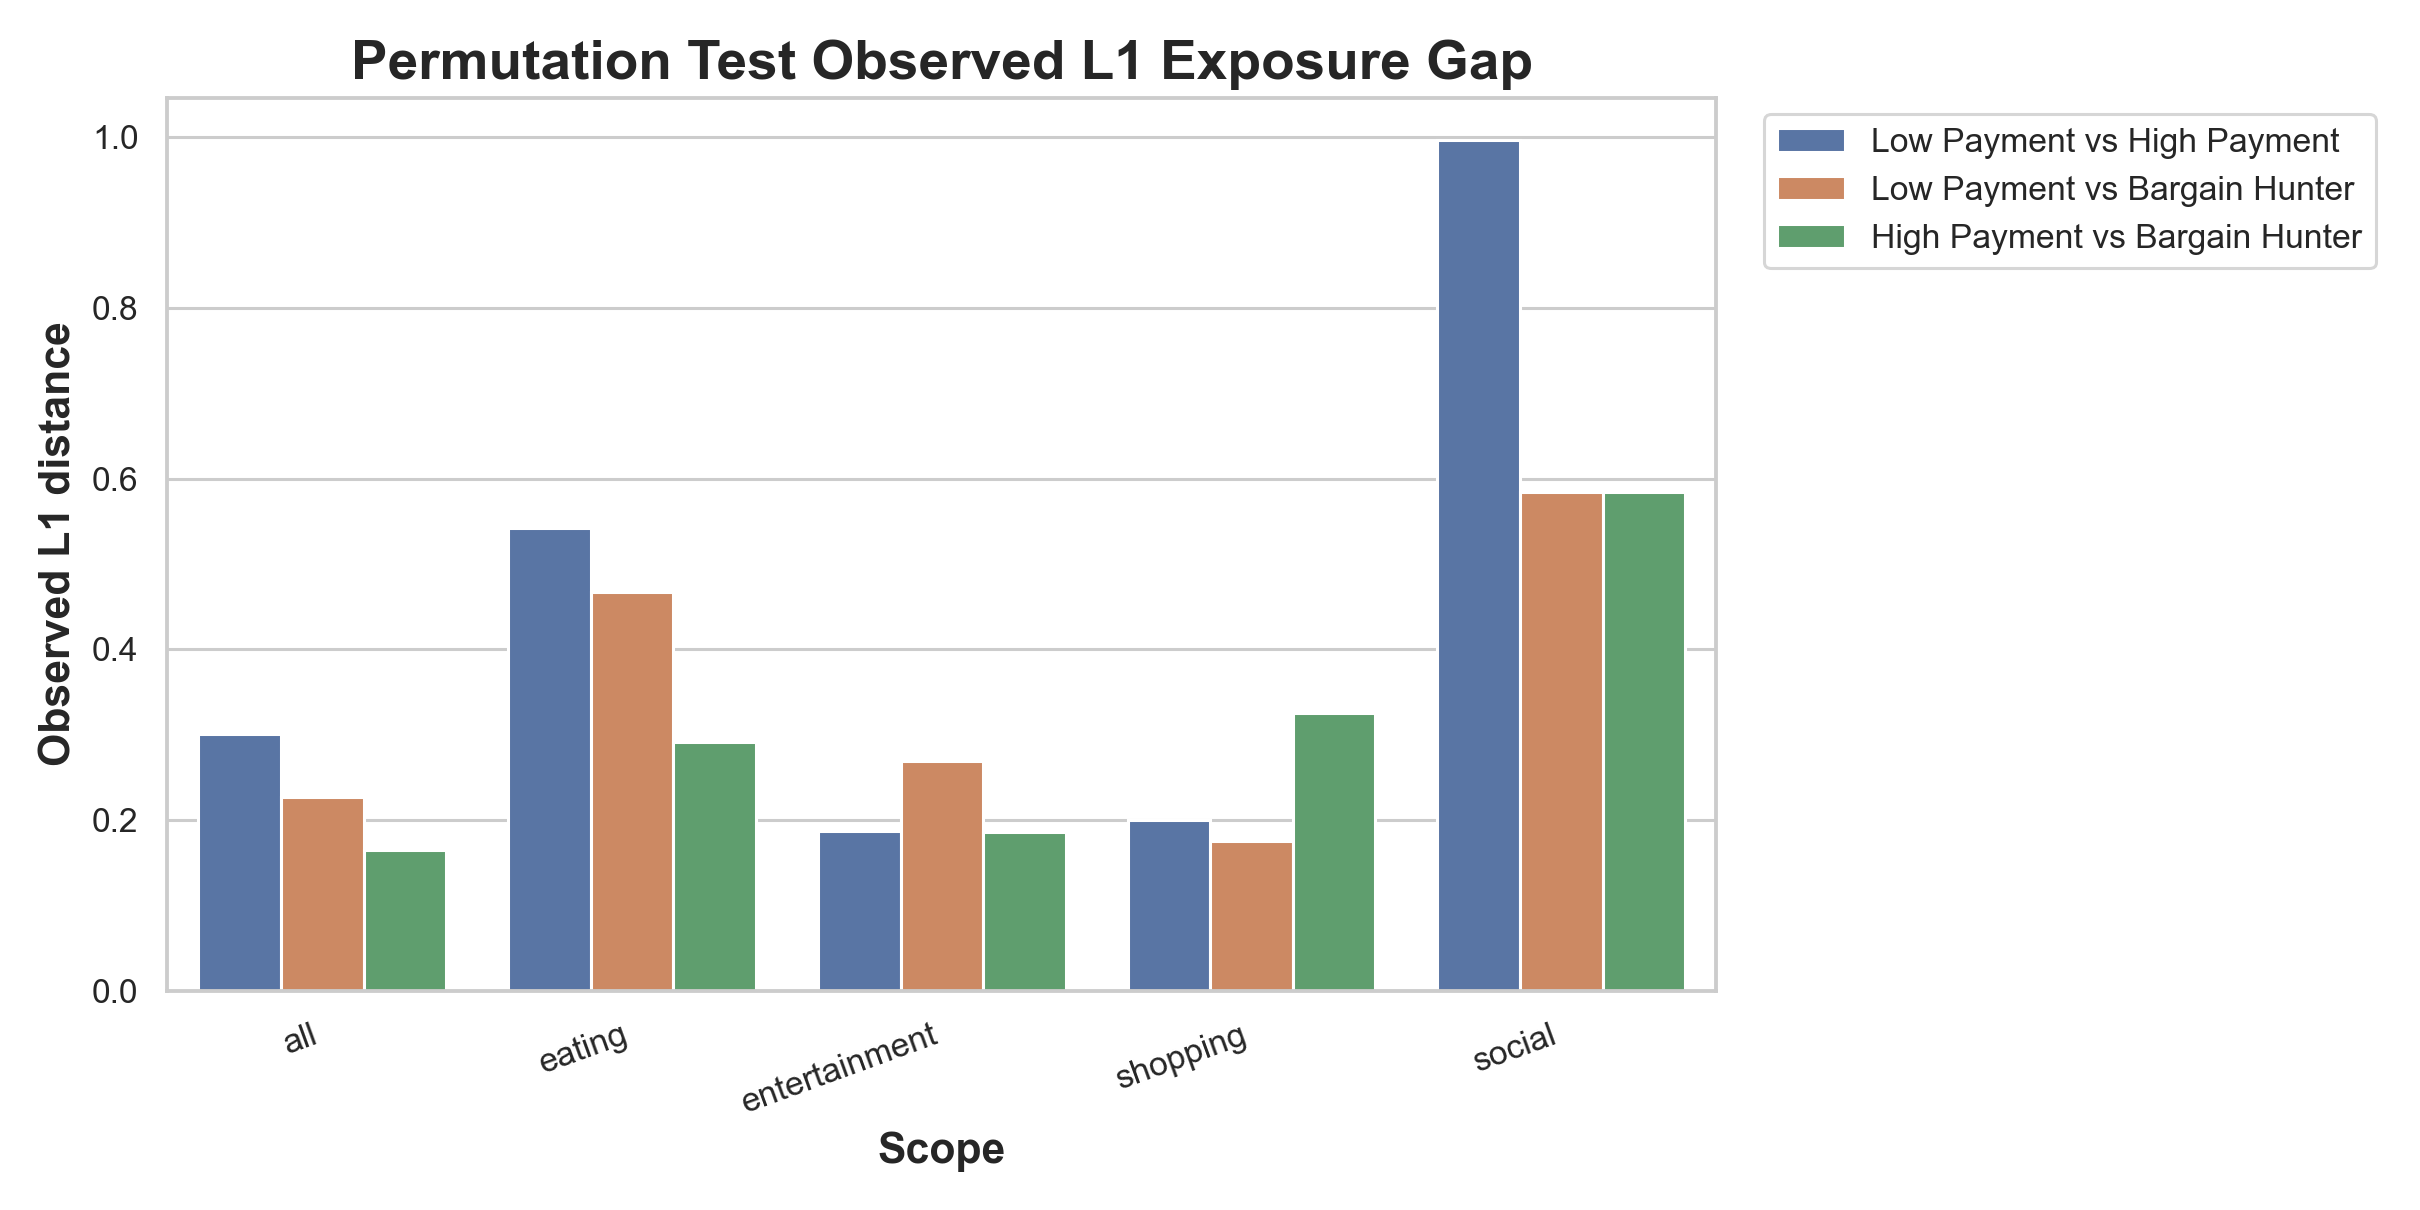
\includegraphics[width=0.95\linewidth]{figures/statistics/permutation_observed_l1_by_scope.png}
    \caption{Representative visualization of observed \(L_1\) exposure distances across comparison scopes based on binarized occurrence \(D_i>0\).}
    \label{fig:method-l1-distance}
\end{figure}

\section{Running Mean Stabilization}

Because a single screenshot can be unstable, the project also examines how exposure estimates change over repeated interaction steps. Early steps may fluctuate because the application has not yet accumulated enough interaction signals, because initial screens contain onboarding or login prompts, or because certain dark pattern mechanisms appear only after specific actions. To observe whether the estimates become more stable, the framework computes a running mean:

\[
\bar{D}_t = \frac{1}{t}\sum_{i=1}^{t} D_i.
\]

The running mean \(\bar{D}_t\) represents the estimated exposure vector after the first \(t\) interaction steps. As \(t\) increases, the estimate incorporates more observations and becomes less sensitive to any single screenshot. These curves are used to examine whether the profile-level exposure estimate stabilizes as more steps are added.

This stabilization analysis evaluates the target 30-step audit budget. If exposure estimates continue to fluctuate heavily after many steps, the audit budget may be insufficient. If the running means gradually stabilize, then the final estimate at the effective trajectory length \(n_{\mathrm{app},A}\) becomes more reliable as a summary of the audited trajectory. In this project, the observed stabilization pattern suggests that repeated interaction is necessary and that the target-budget design provides a more robust estimate than single-state inspection. Nevertheless, stabilization should be understood as empirical support for the audit design, not as proof that all possible long-term exposure patterns have been captured.

\section{Statistical Validation}

The statistical validation layer separates two related but distinct questions.
At the dimension level, the project compares observed exposure values between two profiles with the Mann-Whitney U test.
At the trajectory level, the project uses permutation tests to ask whether the observed profile gap is larger than would be expected after random profile-label reassignment.

The recommended statistical workflow is:
\begin{enumerate}
    \item Compute the observed profile gap, either as a dimension-level difference or as an \(L_1\) distance between profile-level exposure vectors.
    \item Shuffle the profile labels while keeping the DPS observations fixed.
    \item Recompute the gap under the shuffled labels to form a null distribution.
    \item Calculate the permutation \(p\)-value by comparing the observed gap with the null distribution.
    \item Apply multiple-comparison correction to obtain the \(q\)-value.
    \item Report \(L_1\) distance and Cramér's \(V\) as effect-size or association measures.
\end{enumerate}

For the \(q\)-value correction, the report uses Benjamini-Hochberg false-discovery-rate control. This choice is appropriate because the analysis evaluates many profile-dimension and profile-scope comparisons, and the goal is to limit the expected proportion of false discoveries among the reported significant results.

The Mann-Whitney U test is used for dimension-level comparison between two profiles, and its \(p\)-values are then adjusted with the same Benjamini-Hochberg procedure to obtain dimension-level \(q\)-values. The permutation test, by contrast, is reserved for profile-label randomization over the profile-level or category-level exposure gap.

The framework also uses Cramér's \(V\) to measure the strength of association between profile type and DPS exposure. In the reported analysis, Cramér's \(V\) is computed from contingency tables built on binarized DPS occurrence, where each raw score is converted to present versus absent using \(D_i>0\) before tabulation. If future work uses richer ordinal or count scales, the current statistic would require collapsing the positive levels into a binary occurrence indicator or replacing Cramér's \(V\) with an ordinal association measure. In the present report, the binary contingency formulation keeps the statistic aligned with occurrence-rate analysis, while raw means are interpreted as intensity.

Together, Mann-Whitney U tests, permutation tests, Benjamini-Hochberg \(q\)-values, \(L_1\) distance, and Cramér's \(V\) provide complementary evidence. The Mann-Whitney U test evaluates dimension-level separation, the permutation test evaluates whether the observed gap exceeds random reassignment, the \(q\)-value reduces the risk of overinterpreting multiple comparisons, the \(L_1\) distance summarizes the practical magnitude of difference between profiles, and Cramér's \(V\) estimates the association strength between profile type and exposure. By combining these measures, the project avoids relying on a single statistic and provides a more cautious assessment of profile-conditioned dark pattern exposure.

Overall, the differential exposure estimation method treats dark pattern exposure as an empirical, profile-conditioned distribution over interaction states. It does not claim to reveal the internal personalization algorithm of any mobile application. Instead, it measures whether controlled profiles, when interacting with the same applications under reproducible conditions, encounter different patterns of observable dark pattern mechanisms. This framing is consistent with black-box auditing approaches in personalization and platform accountability research, where the goal is to compare observable outputs under controlled conditions rather than to make unsupported claims about internal causality \cite{sandvig2014auditing,hannak2013personalization,srba2023youtube}.

\chapter{System Design and Implementation}

\begin{figure}[htbp]
    \centering
    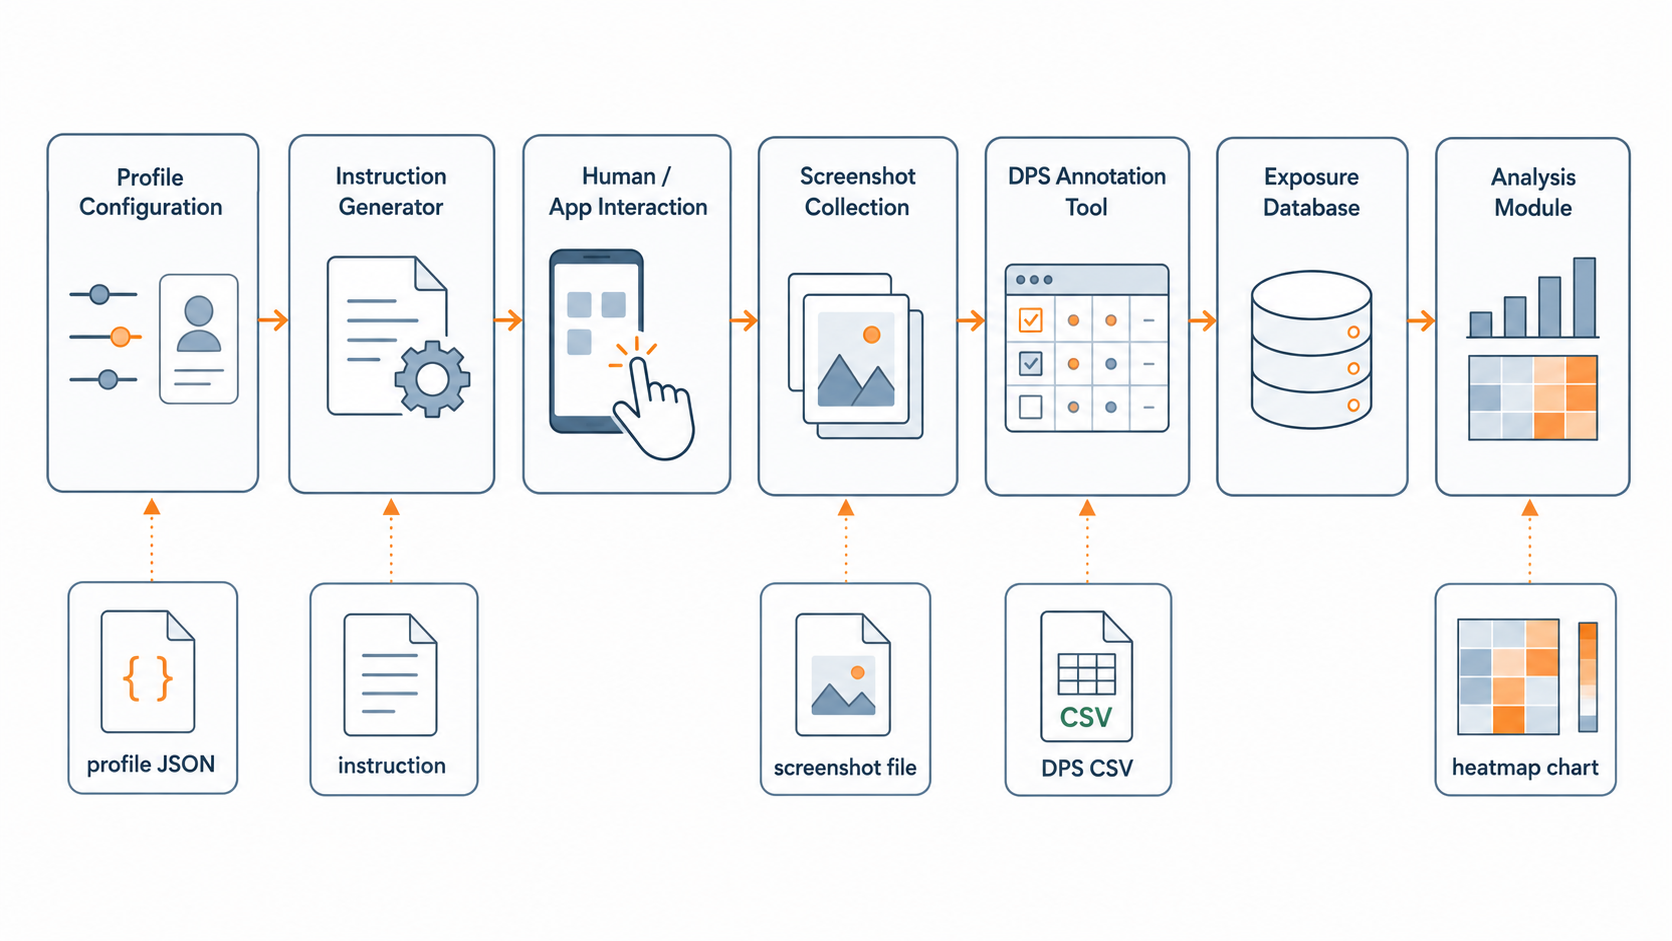
\includegraphics[width=0.95\linewidth]{figures/pictures/system_architecture.png}
    \caption{System Architecture}
    \label{fig:system-architecture}
\end{figure}

\section{Auditing Pipeline Overview}

The system is designed as a profile-aware auditing pipeline that converts abstract user profiles into concrete app interaction trajectories and then into measurable dark-pattern exposure data. Rather than treating dark patterns as static interface elements that can be observed from a single screen, the framework records how exposure emerges during repeated interactions under controlled user assumptions. This design follows the broader logic of black-box auditing, where the internal mechanisms of a platform are not directly accessible, but their observable outputs can be compared under controlled experimental conditions \cite{sandvig2014auditing,srba2023youtube,haroon2023youtubeaudit}.

The pipeline begins with Profile Configuration, where each user profile is defined through behavior probabilities and interest-related keyword distributions. At the beginning of each app-profile run, the workbench loads the configuration, fixes the pseudo-random seed, creates a timestamped run directory, and initializes an empty step record. The system then performs Action Sampling based on the behavior distribution of the selected profile. If the sampled action is search-oriented, the keyword category and concrete keyword are sampled from the profile-specific keyword distribution. The sampled action and keyword are passed to the Instruction Generation module, which translates them into a concrete natural-language interaction instruction. A human operator or semi-automated executor then performs the corresponding App Interaction on a mobile application. After the interaction, the system waits for a fixed delay and collects a Screenshot using a consistent naming and storage convention. The screenshot is then reviewed in the DPS Annotation Tool, where annotators assign seven DPS dimensions: Interface Interference, Friction, Pressure, Contextual Deception, Sneaking, Nagging, and Forced Action. Finally, the annotated step is appended to the Exposure Database and used by the Analysis Module to estimate profile-conditioned exposure and differential exposure patterns.

The complete pipeline can be summarized as:
\[
\text{Profile Configuration} \rightarrow \text{Run Initialization} \rightarrow \text{Action/Keyword Sampling} \rightarrow \text{Instruction Generation} \rightarrow \text{App Interaction} \rightarrow \text{Screenshot Collection} \rightarrow \text{DPS Annotation} \rightarrow \text{Step Persistence} \rightarrow \text{Differential Analysis}.
\]
This implementation structure ensures that the experiment is not merely a collection of screenshots, but a controlled transformation from profile assumptions to interaction traces and then to structured exposure measurements. In the project scale, the framework supports 16 applications, 3 profiles, and 30 interaction steps per profile-app pair, producing 1,440 interaction records and 10,080 DPS labels.

One practical feature of the workflow is that persistence happens after every annotated step rather than only after a full run is completed. The workbench writes both \texttt{steps.jsonl} and \texttt{steps.csv} in the current run directory after each valid step, so interrupted annotation sessions do not invalidate previously collected evidence. The operator can also stop a run early or undo the most recent step before continuing. These controls make the workflow closer to an auditable experiment log than a one-time screenshot collection process.

\section{Repository Structure}
\label{subsec:repository-structure}

The implementation is organized so that profile definitions, generated interaction records, screenshots, analysis scripts, and figures can be traced from the repository rather than from informal experiment notes. The main repository components are:

\begin{itemize}
	\item \texttt{codes/config.json}: profile-independent experiment configuration, including the maximum number of steps, screenshot delay, output directory, and random seed.
	\item \texttt{codes/profiles.json}: profile configuration file containing controlled profile definitions, behavior distributions, keyword pools, and keyword probabilities.
	\item \texttt{codes/main.py}: instruction generator and interactive audit workbench. It samples actions and keywords, generates executable instructions, records screenshots when automatic screenshot support is available, collects DPS annotations, supports undo and early-stop operations, and writes step-level records.
	\item \texttt{results/\{app\}/\{profile\}/\{run\_id\}/screenshots/}: screenshot folder for each app-profile run. Screenshots are stored at the step level and are linked from the corresponding record.
	\item \texttt{results/\{app\}/\{profile\}/\{run\_id\}/steps.csv} and \texttt{steps.jsonl}: annotation files containing the sampled action, keyword category, keyword, generated instruction, screenshot path, DPS scores, timestamp, and optional notes for each interaction step.
	\item \texttt{codes/scripts/analysis\_curve.py}, \texttt{codes/scripts/analysis\_heatmap.py}, and \texttt{codes/scripts/statistical\_tests.py}: analysis scripts used to compute running means, exposure heatmaps, and statistical validation outputs.
	\item \texttt{figures/} and \texttt{figures/statistics/}: figure output folders containing heatmaps, convergence curves, and statistical-test visualizations used in the report.
\end{itemize}

This structure separates configuration, execution, annotation, and analysis. A repeated audit can therefore reuse the same profile configuration and random seed, inspect the generated instructions and screenshots, and regenerate the analysis outputs from the saved step-level annotation files.

\section{Profile Configuration Module}

The profile configuration module defines the experimental conditions under which each audit trajectory is generated. Each profile is stored as a structured configuration rather than as an informal description. This module records the profile name, the behavior probability distribution, the keyword pools, the keyword probabilities, the app category, and the interaction budget. In this project, the three controlled profiles are the high-payment shopping profile, the low-payment browsing profile, and the bargain-hunter profile.

The behavior probability distribution specifies how frequently a profile is expected to perform different interaction actions, such as browsing, searching, visiting a decision-related interface, or returning to a previous page. The keyword pool defines the interest vocabulary available to the profile, while the keyword probabilities determine how likely each keyword is to be selected during search-oriented actions. For example, a high-payment shopping profile may be more associated with high-value electronics or premium product-related keywords, while a bargain-hunter profile may be more associated with discount, coupon, group-buy, or flash-sale terms. These probabilities are not intended to fully model real users. Instead, they create controlled and reproducible approximations of different interest-behavior patterns.

This configuration-based design is important for reproducibility. Since the same profile configuration can be reused across applications and repeated experimental runs, the framework reduces ambiguity in how profiles are operationalized. It also makes profile differences explicit: if two profiles receive different DPS exposure patterns, the comparison can be traced back to controlled differences in their behavior and keyword distributions rather than to undefined user characteristics. Consistent with the ethical scope of the project, demographic attributes are excluded from the configuration. The system therefore audits profile-conditioned exposure through interests and behaviors, not through sensitive personal identities.

In the operational layer, the system may use a finer-grained action vocabulary than the four conceptual categories defined in Chapter~\ref{sec:conceptual-framework}. For example, concrete action tokens can include:

\begin{itemize}
    \item \texttt{visit\_homepage}
    \item \texttt{search\_keyword}
    \item \texttt{browse\_or\_scroll\_page}
    \item \texttt{click\_recommended\_item}
    \item \texttt{like\_or\_favorite}
    \item \texttt{follow\_account}
    \item \texttt{stay\_on\_content}
    \item \texttt{decision\_interface\_visit}
    \item \texttt{close\_popup}
    \item \texttt{back}
\end{itemize}

Before the records are analyzed, these operational actions are mapped back to home, search, browse, and decision so that the behavioral distributions remain comparable at the conceptual level.

\section{Instruction Generation Module}

The instruction generation module serves as the bridge between probabilistic profile configuration and concrete mobile interaction. For each step, the module samples an action from the behavior distribution of the active profile. If the sampled action is a search action, the module further samples a keyword from the profile-specific keyword pool according to the keyword probabilities. The sampled action and keyword are then converted into a natural-language instruction that can be followed during app interaction.

For example, when the sampled action is a keyword search, the generated instruction may be:
\[
\text{`Enter the keyword \{keyword\} in the search box, click the first natural or recommended result, wait for three seconds, and take a screenshot.''}
\]
When the sampled action is browsing or scrolling, the instruction may be:
\[
\text{`Scroll the current page, stop at the first visible promotional or decision-related interface, wait for three seconds, and take a screenshot.''}
\]
These instructions are intentionally concrete. They specify what to do, what kind of interface to stop at, how long to wait, and when to collect evidence. This reduces arbitrary decision-making during interaction and makes the audit procedure easier to repeat.

The current workbench keeps the executor in the loop rather than fully automating app control. The program samples the action, records the instruction, manages screenshots and annotations, and persists the data, while the operator performs the mobile interaction according to the displayed instruction. This implementation boundary avoids relying on brittle app-specific automation scripts and makes the same workflow usable across applications with different layouts. To reduce operator discretion, the instruction text is saved with each step record, so later inspection can verify what the operator was asked to do before the screenshot was captured.

The module does not attempt to infer the internal logic of the application. It only generates external interaction prompts based on controlled profile assumptions. In this sense, the instruction generation module operationalizes profile-conditioned behavior without claiming to simulate the full complexity of real user activity. It provides a practical compromise between experimental control and ecological relevance: the actions are simple enough to standardize, but still close to common app behaviors such as searching, browsing, clicking recommended content, and entering decision-related interfaces.

\section{Screenshot Collection}

Screenshot collection provides the visual evidence for subsequent DPS annotation. After each generated instruction is executed, the framework requires a fixed waiting time before capturing the screen. In this project, the instruction examples use a three-second waiting period. This short delay allows the interface to finish loading dynamic content, recommendation results, pop-ups, or promotional elements before the screenshot is recorded. Although network and device conditions can still introduce variation, using a fixed waiting time improves consistency across steps.

The system also uses a consistent naming convention for screenshots:
\[
\texttt{results/\{app\_name\}/\{profile\_name\}/\{run\_id\}/screenshots/step\_\{step\_id\}.png}
\]
This format encodes the application, profile, run identifier, and step number directly in the file path. It makes screenshots easier to trace, inspect, and match with database records. The run identifier is important because the same app-profile condition may be repeated; without it, repeated runs could overwrite or mix screenshots from different sessions. For example, the screenshot for the seventh step of a high-payment shopping profile in a given app would be stored under that app, profile, and timestamped run directory with the file name \texttt{step\_007.png}.

The implementation supports both automatic and manual screenshot collection. If screenshot automation is available through the local environment, the workbench captures the screen after the configured delay. If automatic capture is unavailable, the workbench prints the expected file path and allows the operator to place a manually captured screenshot there before continuing. This fallback keeps the workflow usable across operating systems and emulator setups while preserving the same path convention in the saved records.

Device and environment consistency are also important. When possible, the same device configuration, account initialization strategy, screen size, network condition, and app version should be maintained across profiles. In the project, controlled conditions include new accounts, cleared histories, comparable app configurations, and profile-specific changes mainly through keyword pools and action distributions. Privacy protection is also necessary during screenshot collection. Screenshots should avoid exposing personal accounts, private messages, payment credentials, precise locations, or other sensitive information. If such information appears, it should be removed, masked, or excluded from the dataset before analysis.

\section{DPS Annotation Tool}

The DPS annotation tool converts visual observations from screenshots into structured dark-pattern exposure labels. For each screenshot, the tool allows annotators to input the seven DPS dimensions: Interface Interference, Friction, Pressure, Contextual Deception, Sneaking, Nagging, and Forced Action. The implementation records numeric scores rather than only binary labels. In particular, Interface Interference can be coded as an ordinal score, Friction can be coded as the extra operation count required to refuse or exit relative to accepting or continuing, and Nagging can be coded as a repeated-interruption count. Pressure, Contextual Deception, Sneaking, and Forced Action are typically coded as binary indicators. When an analysis requires exposure rates, the raw numeric scores can be converted to binary occurrence indicators by applying \(D_i>0\). When an analysis requires intensity, the raw mean score can be used directly.

The tool also supports correction during annotation. Annotators may undo or revise a previous input if they notice an error, and intermediate records can be saved to avoid data loss during long annotation sessions. This is important because the full experiment produces 1,440 interaction records and 10,080 DPS labels. Without intermediate saving and correction support, the annotation process would be more vulnerable to accidental omissions or inconsistent record keeping.

The annotation interface functions as a measurement layer between raw screenshots and statistical analysis. A screenshot alone is not yet an analyzable exposure record. It must first be interpreted according to the DPS framework and converted into structured labels or scores. For example, a pop-up that visually emphasizes a paid option may be annotated as Interface Interference; a countdown or scarcity message may be annotated as Pressure; a screen that requires login or agreement before continuing may be annotated as Forced Action. The tool therefore standardizes how visual interface evidence becomes data for profile-conditioned exposure estimation while still preserving enough score detail for later robustness checks.

\section{Exposure Database}

The exposure database stores the complete interaction and annotation record for the audit. Each row corresponds to one interaction step under a specific app-profile condition. The database is designed to preserve both the experimental context and the annotated outcome, so that each DPS label can be traced back to its application, profile, action, keyword, screenshot, and annotation notes.

Table~\ref{tab:exposure_database_schema} shows the analysis-ready data schema used by the framework. The current raw output files use closely related implementation names such as \texttt{app}, \texttt{profile\_id}, \texttt{step}, and \texttt{note}; these correspond to \texttt{app\_name}, \texttt{profile}, \texttt{step\_id}, and \texttt{notes} in the normalized schema below. The \texttt{app\_category} field is derived from the repository's app-category mapping used for category-level analysis.

	\begin{table}[htbp]
	\centering
	\caption{Exposure database schema.}
	\label{tab:exposure_database_schema}
	\begin{tabular}{ll}
	\hline
	\textbf{Field} & \textbf{Description} \\
	\hline
	\texttt{app\_name} & Name of the audited mobile application \\
	\texttt{app\_category} & Category of the application, such as shopping or food delivery \\
	\texttt{profile} & Controlled profile used in the interaction step \\
	\texttt{step\_id} & Step number within the profile-app trajectory \\
	\texttt{action} & Action sampled from the profile behavior distribution \\
	\texttt{category} & Keyword category sampled for search-oriented actions \\
	\texttt{keyword} & Sampled keyword if the action involves search \\
	\texttt{instruction} & Natural-language instruction shown to the operator \\
	\texttt{screenshot\_path} & File path of the collected screenshot \\
	\texttt{I} & Interface Interference score \\
	\texttt{F} & Friction score or operation-count difference \\
	\texttt{P} & Pressure score or indicator \\
	\texttt{C} & Contextual Deception score or indicator \\
	\texttt{S} & Sneaking score or indicator \\
	\texttt{N} & Nagging score or interruption count \\
	\texttt{FA} & Forced Action score or indicator \\
	\texttt{timestamp} & Time at which the record was created or annotated \\
	\texttt{notes} & Optional comments for ambiguous or notable cases \\
	\hline
	\end{tabular}
	\end{table}

This schema supports both traceability and aggregation. At the lowest level, researchers can inspect a single screenshot and its labels. At a higher level, the same records can be grouped by profile, app, app category, action type, or DPS dimension. The database therefore acts as the central connection between implementation and analysis.

\section{Analysis Module}

The analysis module computes exposure estimates and differential exposure statistics from the exposure database. At the profile level, it estimates profile-conditioned exposure \(E(D \mid A)\), where \(A\) denotes a controlled profile and \(D\) denotes a DPS dimension or DPS vector. Depending on the analysis mode, \(D\) can refer either to the raw DPS score or to a binary occurrence variable \(1[D_i>0]\). The former summarizes exposure intensity, while the latter summarizes how frequently a profile encounters each type of dark-pattern exposure across its interaction trajectory. At the app level, the module aggregates DPS labels within each application. At the category level, it further groups applications into broader categories, allowing the project to examine whether certain app categories are associated with consistently higher exposure in specific DPS dimensions.

The module also computes pairwise exposure differences:
\[
\Delta(A_i, A_j) = E(D \mid A_i) - E(D \mid A_j).
\]
This comparison is used to examine whether two controlled profiles receive different dark-pattern exposure patterns under comparable experimental conditions. The framework does not interpret such differences as direct causal proof of personalization. Instead, it treats them as observable profile-conditioned exposure gaps that may be associated with differences in behavior distributions, keyword interests, app responses, or decision-interface triggers.

Several visualization and statistical components are included. Heatmaps display exposure patterns across profiles, applications, categories, and DPS dimensions. Running mean convergence curves track how exposure estimates change as interaction steps accumulate, helping assess whether the estimates gradually stabilize over repeated interactions. The representative heatmaps and statistical validation plots are reported in Chapter~\ref{chap:results}, with the full visualization set collected in Appendix~\ref{app:full-heatmaps}.

For statistical validation, the analysis module supports permutation tests, q-values for multiple-testing correction, L1 distance, Cramér’s V, Welch's \(t\)-tests, and Mann--Whitney \(U\) tests. Permutation tests compare observed profile gaps against gaps obtained under randomized profile assignments. Q-values reduce the risk of overinterpreting repeated significance tests across multiple DPS dimensions or app categories. L1 distance measures the magnitude of difference between DPS exposure vectors, while Cramér’s V provides an association measure between profile type and exposure labels. The chi-square contingency analysis can be run in binary mode, where each nonzero DPS score counts as one occurrence, or in score mode, where raw DPS scores are summed. Together, these outputs allow the report to discuss both statistical evidence and practical exposure differences without relying on a single metric.

\chapter{Experimental Design}
\label{sec:experimental-design}

This section describes the experimental design used to audit whether controlled user profiles receive different levels or types of dark pattern exposure in mobile applications. The purpose of the experiment is not to fully reproduce the complete diversity of real-world mobile app usage, but to create a controlled and reproducible setting in which profile-conditioned exposure can be compared across applications. Following the logic of black-box platform auditing, the experiment treats each mobile application as an externally observable system: the internal ranking, recommendation, promotion, and interface-generation mechanisms are not directly inspected, but their visible outputs are recorded through repeated profile-conditioned interactions \cite{sandvig2014auditing,hannak2013personalization,srba2023youtube}.

\section{Application Selection}
\label{subsec:application-selection}

The experiment audits sixteen mobile applications selected from common user-facing service categories, including e-commerce, food delivery, lifestyle services, content platforms, and local services. These categories were chosen because they contain frequent decision points and commercial interaction opportunities. In such applications, users are often asked to search, browse, select, compare, register, subscribe, join membership programs, accept promotional offers, enter payment flows, or respond to pop-ups. These interaction contexts are especially relevant for studying deceptive or manipulative interface mechanisms because dark patterns often appear at moments where user decisions have commercial or privacy-related consequences \cite{gray2018darkpatterns,mathur2019darkpatterns}.

The selected categories also contain a mixture of recommendation flows and transactional interfaces. E-commerce and food-delivery applications frequently use coupons, limited-time promotions, membership discounts, bundled offers, and checkout-related prompts. Lifestyle and local-service applications often include login prompts, location requests, membership registration, service booking flows, and payment-related interfaces. Content platforms may rely more heavily on recommendation feeds, attention retention mechanisms, nagging prompts, and repeated requests for account binding or notification permissions. Together, these categories provide a practical testbed for examining whether different profiles encounter different forms of interface interference, pressure, forced action, or other DPS dimensions.

The application set should therefore be understood as a controlled sample rather than a statistically representative sample of all mobile applications. The goal is to cover several high-frequency app categories in which decision architecture is visible and repeatedly encountered. This design allows the project to compare exposure patterns across profile types while still keeping the experiment feasible for a course-scale audit.

\section{Profile Setup}
\label{subsec:profile-setup}

The experiment uses three controlled profiles: a high-payment shopping profile, a low-payment browsing profile, and a bargain-hunter profile. These profiles are not intended to represent demographic groups or real individuals. Instead, they are experimental instruments designed to introduce controlled differences in interests and interaction behavior. This distinction is important because the project focuses on profile-conditioned exposure while avoiding direct demographic attributes such as age, gender, income, or identity categories. The profile design follows the broader idea in user modeling that users may be represented through interests and behaviors, but it operationalizes these components in a simplified and reproducible way \cite{eke2019userprofiling,purificato2024usermodeling}.

The high-payment shopping profile is used to simulate a user who frequently searches for or browses higher-value goods and is more willing to enter decision-related interfaces such as product detail pages, membership prompts, or checkout flows. The low-payment browsing profile is used to simulate a more casual user who spends more time browsing or scrolling and less time entering payment-related contexts. The bargain-hunter profile is used to simulate a user who is sensitive to promotions, discounts, coupons, flash sales, and reward mechanisms. In the actual audit process, the differences among these profiles are introduced through profile-specific behavior probabilities and keyword pools. For example, when a search action is sampled, the keyword is drawn from the corresponding profile's keyword distribution. When a browsing or decision-interface action is sampled, the instruction reflects the behavioral tendency of that profile.

This setup allows the experiment to ask whether interface exposure differs when the same applications are approached through different controlled behavioral patterns. The profiles should not be interpreted as complete psychological models of users. Rather, they serve as reproducible experimental conditions for comparing dark pattern exposure under different interest-behavior assumptions.

\section{Interaction Budget and Dataset Scale}
\label{subsec:interaction-budget}

For each application and each profile, the audit runs for thirty interaction steps. With sixteen applications and three profiles, this produces:
\[
16 \ \text{apps} \times 3 \ \text{profiles} \times 30 \ \text{steps} = 1{,}440 \ \text{interaction records}.
\]
Each interaction record is annotated using the seven-dimensional DPS vector:
\[
DPS = [I, F, P, C, S, N, FA],
\]
where \(I\) denotes Interface Interference, \(F\) denotes Friction, \(P\) denotes Pressure, \(C\) denotes Contextual Deception, \(S\) denotes Sneaking, \(N\) denotes Nagging, and \(FA\) denotes Forced Action. Since each record contains seven DPS labels, the full dataset contains:
\[
1{,}440 \times 7 = 10{,}080 \ \text{DPS labels}.
\]

The choice of thirty steps reflects a balance between feasibility and repeated exposure estimation. A single screenshot would be too fragile because dark pattern exposure may depend on timing, page state, recommendation flow, login status, promotion availability, or the user's previous actions within the app. Repeated interactions provide a more stable basis for estimating profile-conditioned exposure \(E(D \mid A)\). At the same time, the audit remains small enough to be manually executed and annotated within the constraints of a course project. The running mean convergence curves introduced later in the report are used to examine whether exposure estimates gradually stabilize as more interaction steps are collected. In this sense, the fixed interaction budget is not assumed to be perfect; instead, it is treated as an experimental design choice whose stability can be evaluated empirically.

\section{Experimental Controls}
\label{subsec:experimental-controls}

The experiment uses several controls to reduce unrelated noise and improve comparability across profiles. When possible, new accounts are created for the audit so that prior user histories do not dominate the observed app behavior. Browsing histories, search histories, and other locally stored traces are cleared before the experiment where the application and device environment allow it. The same device configuration is used across profiles, and the same app version is maintained when possible. These controls are important because mobile applications may adapt their interfaces based on device settings, account histories, location permissions, app version, cached behavior, or previous search and browsing activity.

The experiment also keeps the number of interaction steps constant across all app-profile pairs. Each profile receives thirty steps in each application, so exposure differences are not caused by one profile simply interacting more than another. A fixed waiting time is used before screenshots are captured, so that dynamic interface elements have time to load and the screenshot timing is more consistent. The same DPS annotation rules are applied across all records. This helps ensure that a label such as pressure, friction, or forced action is interpreted according to the same criteria regardless of the application or profile.

Most importantly, the intended differences among profiles are introduced only through behavior probabilities and keyword pools. The device, annotation framework, interaction budget, and screenshot procedure are kept as similar as possible. This does not eliminate all possible confounding factors, since mobile applications are dynamic systems and may change over time. However, these controls reduce unrelated variation and make the comparison more focused on the relationship between controlled profile behavior and observed dark pattern exposure.

\section{Random Seed and Sampling Reproducibility}
\label{subsec:random-seed}

Action and keyword sampling are controlled by the random seed in \texttt{codes/config.json}. In the current implementation, \texttt{random\_seed} is set to \texttt{20260603}, and \texttt{codes/main.py} initializes the sampling generator with this value before the audit loop begins. Under the same profile configuration, keyword pool, app order, and execution sequence, this seed makes the generated sequence of sampled actions and sampled keywords reproducible.

The seed controls the instruction generation stage, not the full mobile-app environment. App interfaces may still vary because of network timing, account state, app updates, server-side recommendation changes, location permissions, or promotional campaigns. For this reason, reproducibility in this project means that the experimental inputs and generated audit instructions can be regenerated, while the observed screen outputs remain subject to the normal variability of black-box mobile applications. To support later inspection, each executed step is saved with its action, keyword, screenshot path, timestamp, DPS labels, and notes.

\section{Audit Procedure}
\label{subsec:audit-procedure}

The audit procedure is designed as a repeated interaction loop. For each application-profile pair, the system loads the configured profile, samples an action, generates a concrete instruction, records the resulting interface state, annotates the screenshot, and updates the exposure estimate. The procedure is deliberately explicit so that another auditor can reproduce the experimental inputs and check each saved observation against the corresponding screenshot.

For clarity, the procedure can be summarized as follows:

\begin{enumerate}
    \item Create a new account for the target application when feasible, or clean the existing account, browsing history, search history, cache, and profile traces where the app allows it.
    \item Load the profile configuration from the profile file, including the behavior probability distribution and keyword pool.
    \item Sample an action from the profile-conditioned behavior distribution using the configured random seed.
    \item If the sampled action is search-oriented, sample a keyword from the profile-specific keyword pool.
    \item Generate an executable natural-language instruction from the sampled action and keyword.
    \item Execute the instruction manually or semi-automatically in the mobile application.
    \item Wait for the fixed number of seconds specified in the configuration before collecting evidence.
    \item Capture a screenshot of the resulting interface state and save it in the run-specific screenshot folder.
    \item Annotate the screenshot using the seven-dimensional DPS vector \([I,F,P,C,S,N,FA]\).
    \item Save the step-level record, including \texttt{app\_name}, \texttt{app\_category}, \texttt{profile}, \texttt{step\_id}, \texttt{action}, \texttt{keyword}, \texttt{screenshot\_path}, \texttt{I}, \texttt{F}, \texttt{P}, \texttt{C}, \texttt{S}, \texttt{N}, \texttt{FA}, \texttt{timestamp}, and \texttt{notes}.
    \item Update the running mean exposure estimate for each DPS dimension using all records collected so far in the current trajectory.
    \item Repeat the process until thirty steps are completed for the current application-profile pair.
\end{enumerate}

This step-by-step procedure supports reproducibility because each record can be traced back to a profile, an action, a keyword if applicable, and a screenshot. It also makes the audit trajectory explicit, allowing later analysis to estimate exposure not only from isolated screenshots but from repeated interaction sequences.

\section{Annotation Reliability Considerations}
\label{subsec:annotation-reliability}

The project relies on manual annotation of screenshots, which is both a strength and a limitation. Manual annotation allows the auditor to interpret interface context, visual hierarchy, button wording, pop-up behavior, and decision flow in ways that simple automated detectors may miss. This is especially useful for dimensions such as Contextual Deception, Friction, and Pressure, where the meaning of an interface element may depend on the surrounding task context. At the same time, manual annotation introduces the possibility of inconsistency, subjectivity, and fatigue. Different annotators may disagree about whether a particular interface counts as pressure, whether a login prompt should be labeled as forced action, or whether a confusing layout rises to the level of interface interference.

To reduce inconsistency, the report defines clear DPS guidelines and applies the same rules across all applications and profiles. Ambiguous cases can be reviewed after initial annotation, and difficult examples can be discussed to refine the interpretation of each DPS dimension. The annotation process should therefore be understood as rule-guided manual coding rather than informal impressionistic judgment. Nevertheless, the current project does not claim to fully solve the reliability problem. Because it is a course-scale audit, it does not include a full multi-annotator reliability study.

Future work should improve this part of the framework by involving multiple annotators and calculating inter-annotator agreement metrics such as Cohen's Kappa. Multiple annotators would make it possible to identify unstable DPS categories, revise unclear annotation rules, and distinguish robust exposure differences from differences caused by coding variation. In a larger study, disagreement analysis could also become a useful methodological tool: if certain interface patterns repeatedly produce annotation disagreement, this may indicate that the boundary between acceptable persuasion and deceptive design is itself ambiguous. For the present project, the annotation design emphasizes transparency, consistency, and reproducible comparison while acknowledging that stronger reliability validation remains an important direction for future work.

\chapter{Results}
\label{chap:results}

\begin{figure}[htbp]
    \centering
    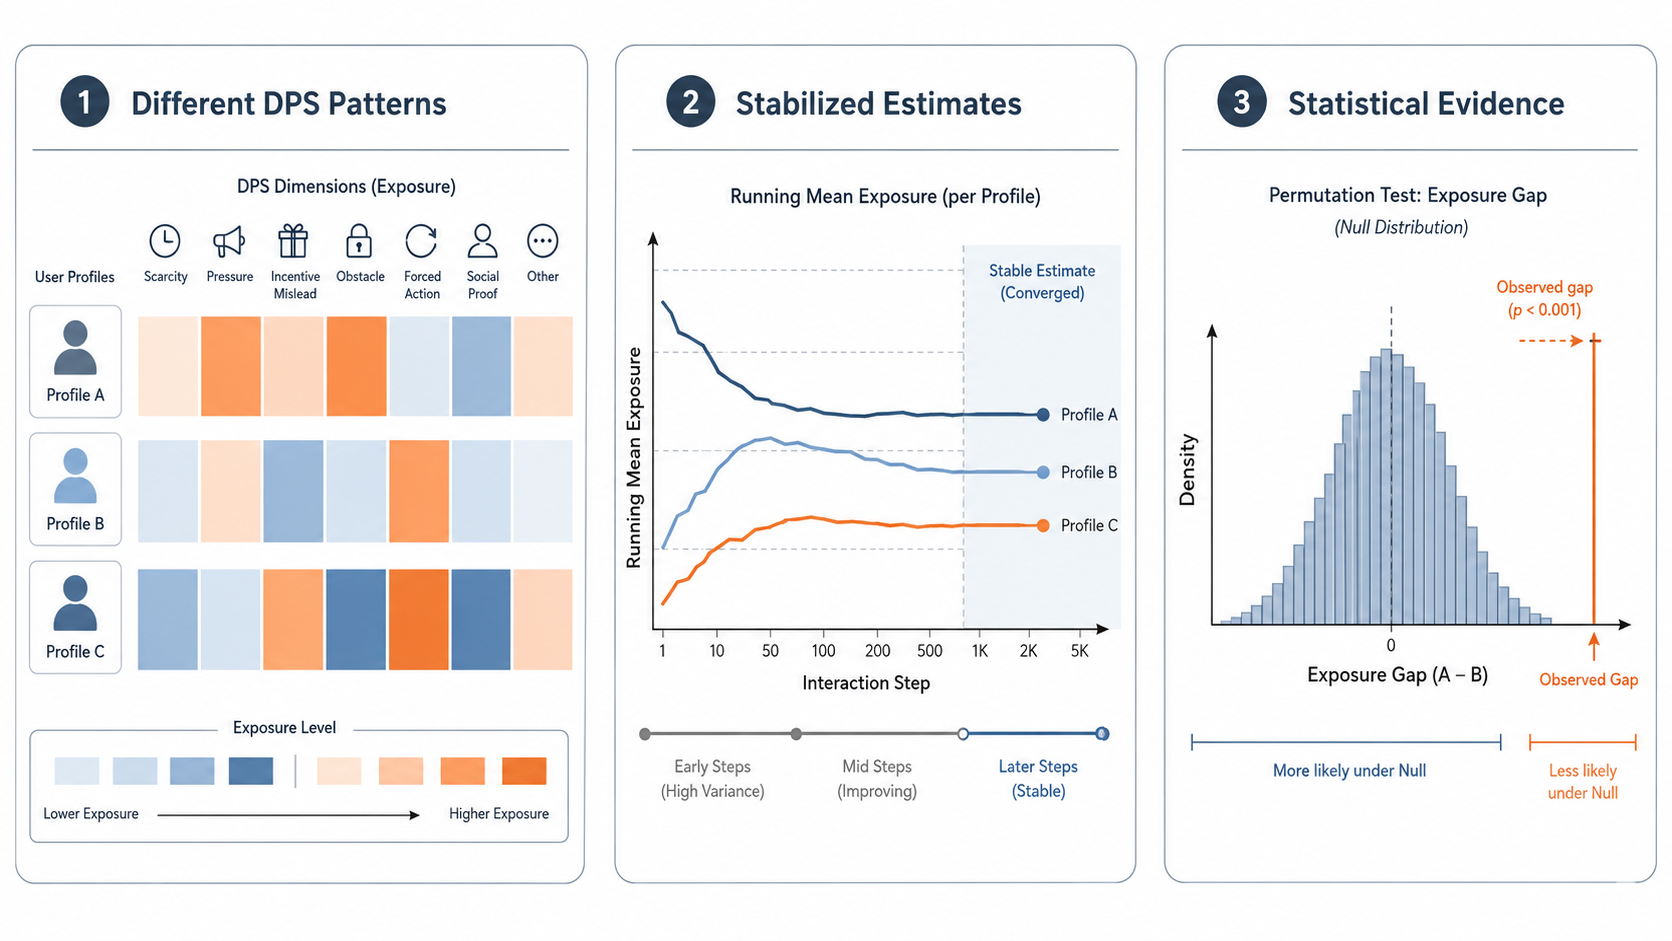
\includegraphics[width=0.95\linewidth]{figures/pictures/results_dashboard_overview.png}
    \caption{Dashboard Overview}
    \label{fig:dashboard_overview}
\end{figure}


\section{Overview of Results}

This section reports the empirical results of the profile-aware dark pattern auditing experiment. The repository contains 1,403 interaction records from 16 mobile applications and three controlled user profiles. The protocol was designed around 30 interaction steps for each app-profile pair; in the archived results, the observed trajectory length ranges from 20 to 30 steps because a small number of runs ended before the planned length. Since each interaction record was annotated with the seven-dimensional DPS vector, the resulting dataset contains 9,821 dimension-level DPS labels. These labels provide the basis for estimating profile-conditioned dark pattern exposure, comparing exposure differences across profiles, and examining whether observed differences are likely to reflect systematic profile-dependent variation rather than random fluctuation.

\begin{table}[htbp]
    \centering
    \caption{Summary of the experimental result dataset.}
    \label{tab:results-overview}
    \begin{tabular}{ll}
        \toprule
        Item & Value \\
        \midrule
        Number of apps & 16 \\
        Number of profiles & 3 \\
        Steps per app-profile pair & Planned: 30; observed: 20--30 \\
        Total interaction records & 1,403 \\
        Total DPS labels & 9,821 \\
        DPS dimensions & I, F, P, C, S, N, FA \\
        \bottomrule
    \end{tabular}
\end{table}

Overall, the results suggest that dark pattern exposure is not uniform across controlled user profiles. Different profiles produce visibly different DPS distributions, and these differences appear across multiple forms of analysis. The heatmaps show that the average exposure intensity varies not only across applications and app categories, but also across user profiles. The running mean convergence curves further indicate that exposure estimates gradually stabilize as interaction steps accumulate, suggesting that the results are not driven by isolated screenshots or single-step observations. Finally, the statistical validation metrics, including Mann-Whitney U q-values, permutation tests, L1 distance, and Cramér's V, provide converging evidence that profile type is associated with measurable differences in dark pattern exposure.

The main empirical pattern is that commercially oriented profiles, especially the high-payment shopping profile and the bargain-hunter profile, tend to encounter stronger exposure in dimensions related to interface interference and pressure. This does not imply that platforms deliberately single out those profiles with dark patterns. A more cautious interpretation is that profile-conditioned behavior changes the interaction trajectory, and different trajectories lead users into different interface regions where dark patterns are more or less likely to appear. For example, a user who frequently enters purchase, membership, coupon, or payment interfaces naturally observes more decision-stage interface designs than a user who mainly browses information feeds. In this sense, the results support the central claim of this project: dark pattern exposure should be analyzed as a profile-conditioned distribution along interaction trajectories, rather than as a static property of an application.

\section{Finding 1: Different Profiles Show Different DPS Patterns}

\paragraph{Result.}
The three controlled profiles show different DPS exposure patterns. At the aggregate level, the high-payment shopping profile has the highest mean DPS exposure, followed by the bargain-hunter profile and the low-payment browsing profile. The difference is not uniform across dimensions: the largest profile-level changes appear in Interface Interference, Pressure, and Forced Action, while Contextual Deception and Sneaking remain comparatively low in the overall dataset.
However, simply looking at the overall averages is not sufficiently distinctive on its own. The profile gap becomes much clearer when the analysis is broken down by application category, especially in social and food-delivery applications.

\begin{table}[htbp]
    \centering
    \caption{Profile-level mean DPS exposure across all audited applications.}
    \label{tab:profile-mean-dps}
    \footnotesize
    \begin{tabular}{lrrrrrrrr}
        \toprule
        Profile & I & F & P & C & S & N & FA & Total / Mean \\
        \midrule
        High-payment shopping & 0.638 & 0.165 & 0.522 & 0.030 & 0.030 & 0.163 & 0.717 & 2.264 / 0.323 \\
        Low-payment browsing & 0.518 & 0.130 & 0.477 & 0.022 & 0.028 & 0.117 & 0.672 & 1.963 / 0.280 \\
        Bargain hunter & 0.606 & 0.173 & 0.475 & 0.051 & 0.015 & 0.135 & 0.704 & 2.161 / 0.309 \\
        \bottomrule
    \end{tabular}%
\end{table}

\paragraph{Evidence.}
Table~\ref{tab:profile-mean-dps} reports the mean DPS values computed from the archived step-level CSV files. Figure~\ref{fig:mean-exposure-all} provides the corresponding heatmap. In this heatmap, rows represent controlled profiles and columns represent the seven DPS dimensions: Interface Interference, Friction, Pressure, Contextual Deception, Sneaking, Nagging, and Forced Action. The color intensity of each cell represents the average exposure score for a profile-dimension combination. A darker or more saturated cell therefore indicates stronger average exposure in that DPS dimension under a particular profile condition.

\begin{figure}[htbp]
    \centering
    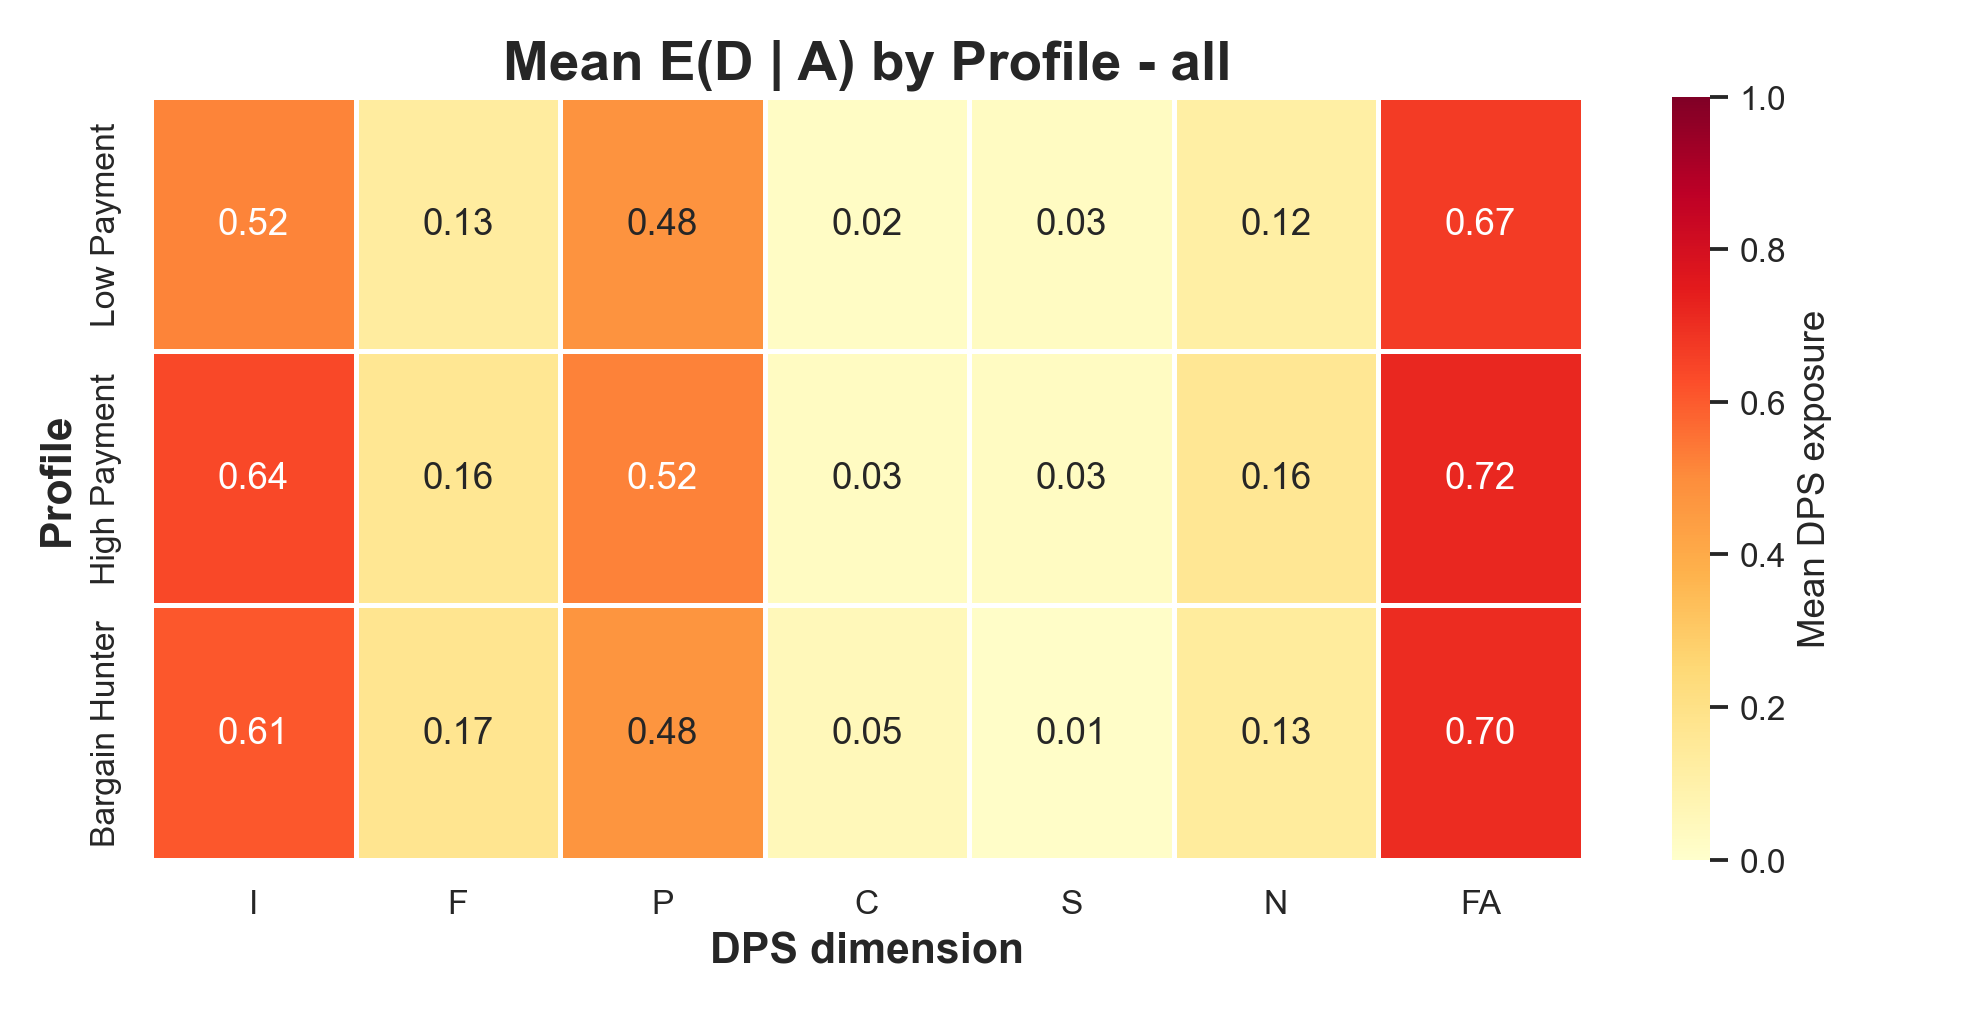
\includegraphics[width=0.95\linewidth]{figures/statistics/heatmap_mean_exposure_all.png}
    \caption{Mean DPS exposure across all audited applications and controlled profiles.}
    \label{fig:mean-exposure-all}
\end{figure}

\paragraph{Food-delivery evidence.}
The category-level result for food-delivery applications shows a clearer profile gap than the global average alone. Table~\ref{tab:eating-mean-dps} summarizes the mean DPS exposure for the food-delivery category across all audited applications in that scope. Figure~\ref{fig:mean-exposure-eating} shows the corresponding heatmap, where the separation between profiles is especially visible in Pressure and Forced Action.

\begin{table}[htbp]
    \centering
    \caption{Profile-level mean DPS exposure for food-delivery applications.}
    \label{tab:eating-mean-dps}
    \footnotesize
    \begin{tabular}{lrrrrrrrr}
        \toprule
        Profile & I & F & P & C & S & N & FA & Total / Mean \\
        \midrule
        High-payment shopping & 0.442 & 0.058 & 0.542 & 0.000 & 0.033 & 0.183 & 0.975 & 2.233 / 0.319 \\
        Low-payment browsing & 0.242 & 0.092 & 0.600 & 0.000 & 0.008 & 0.108 & 0.825 & 1.875 / 0.268 \\
        Bargain hunter & 0.442 & 0.100 & 0.483 & 0.000 & 0.000 & 0.075 & 0.925 & 2.025 / 0.289 \\
        \bottomrule
    \end{tabular}%
\end{table}

\begin{figure}[htbp]
    \centering
    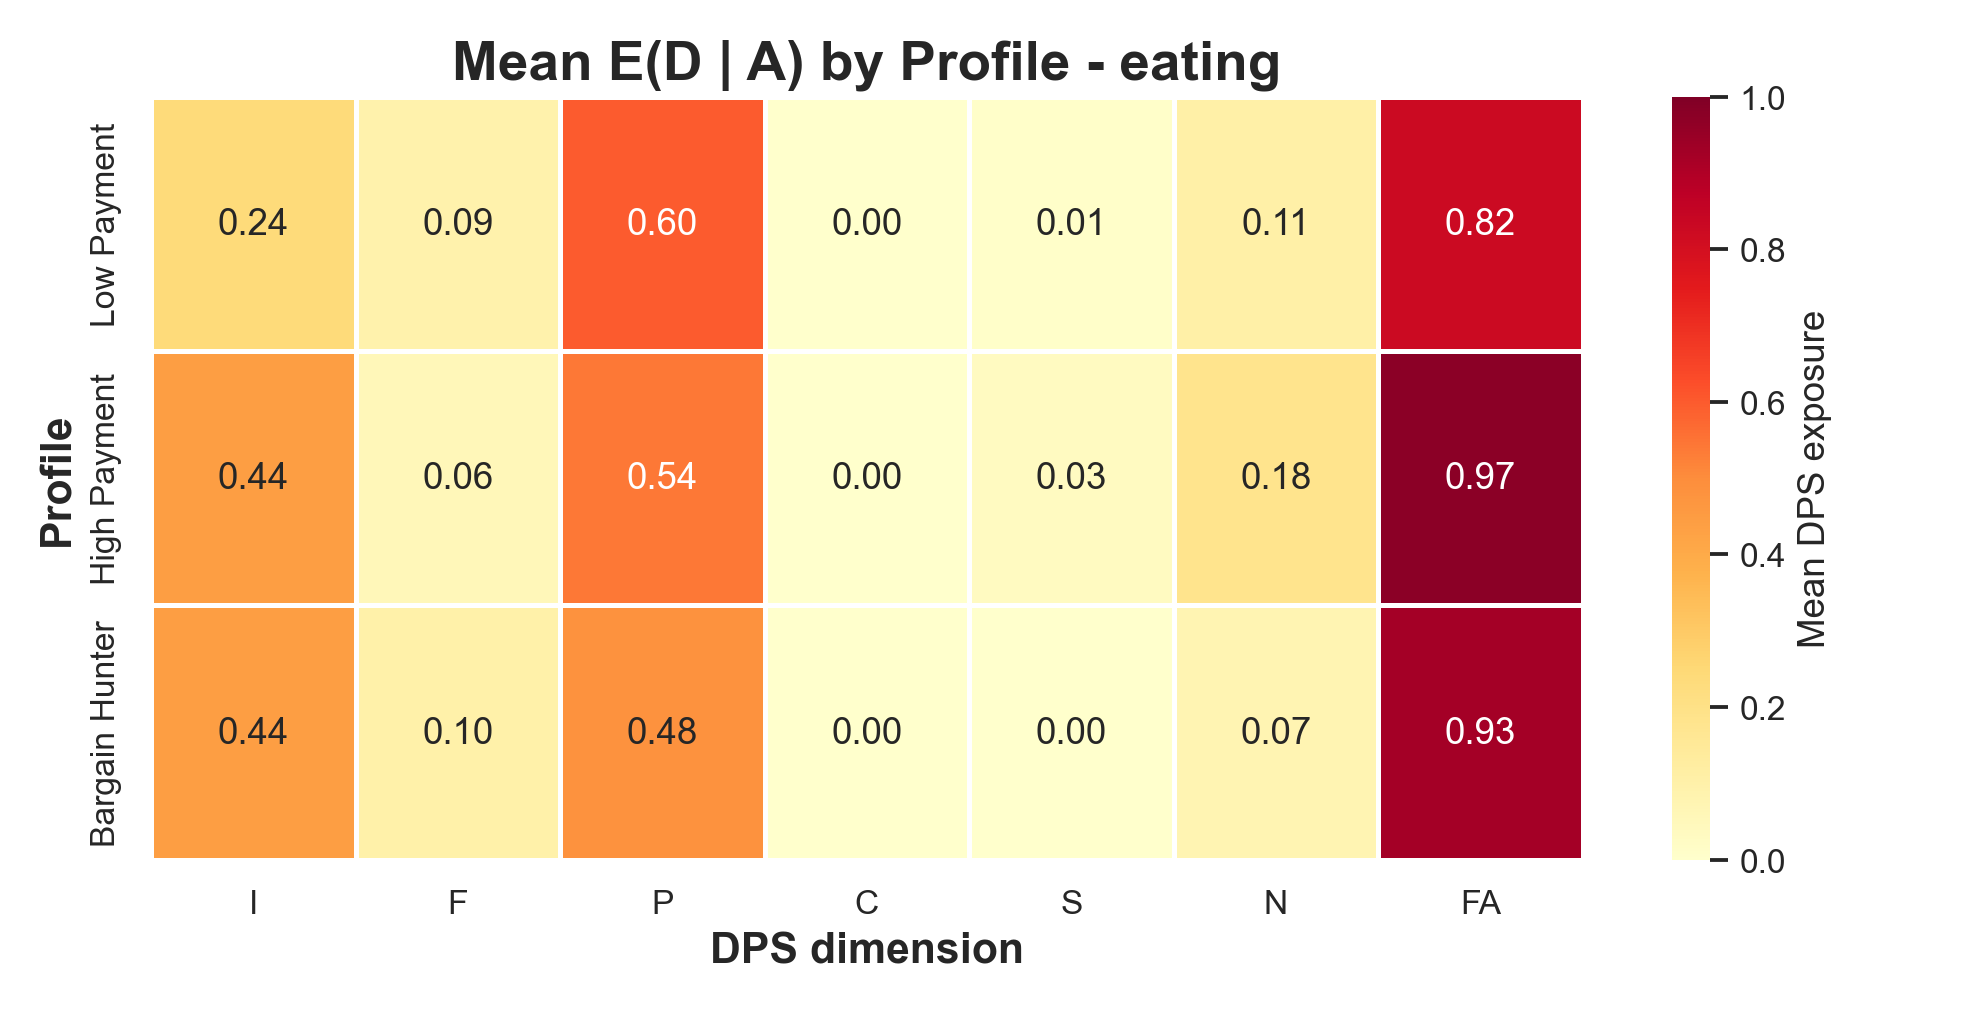
\includegraphics[width=0.95\linewidth]{figures/statistics/heatmap_mean_exposure_eating.png}
    \caption{Mean DPS exposure heatmap for food-delivery and eating-related applications.}
    \label{fig:mean-exposure-eating}
\end{figure}

\paragraph{Social evidence.}
Social applications show the clearest category-level separation among the audited domains. Table~\ref{tab:social-mean-dps} summarizes the mean DPS exposure for social applications across the audited sample. Figure~\ref{fig:mean-exposure-social} shows the corresponding heatmap, where Interface Interference, Friction, and Nagging differ visibly across profiles.

\begin{table}[htbp]
    \centering
    \caption{Profile-level mean DPS exposure for social applications.}
    \label{tab:social-mean-dps}
    \footnotesize
    \begin{tabular}{lrrrrrrrr}
        \toprule
        Profile & I & F & P & C & S & N & FA & Total / Mean \\
        \midrule
        High-payment shopping & 1.319 & 0.451 & 0.504 & 0.053 & 0.053 & 0.389 & 0.044 & 2.814 / 0.402 \\
        Low-payment browsing & 0.958 & 0.250 & 0.333 & 0.083 & 0.100 & 0.242 & 0.083 & 2.050 / 0.293 \\
        Bargain hunter & 1.089 & 0.384 & 0.473 & 0.161 & 0.045 & 0.286 & 0.080 & 2.473 / 0.353 \\
        \bottomrule
    \end{tabular}%
\end{table}

\begin{figure}[htbp]
    \centering
    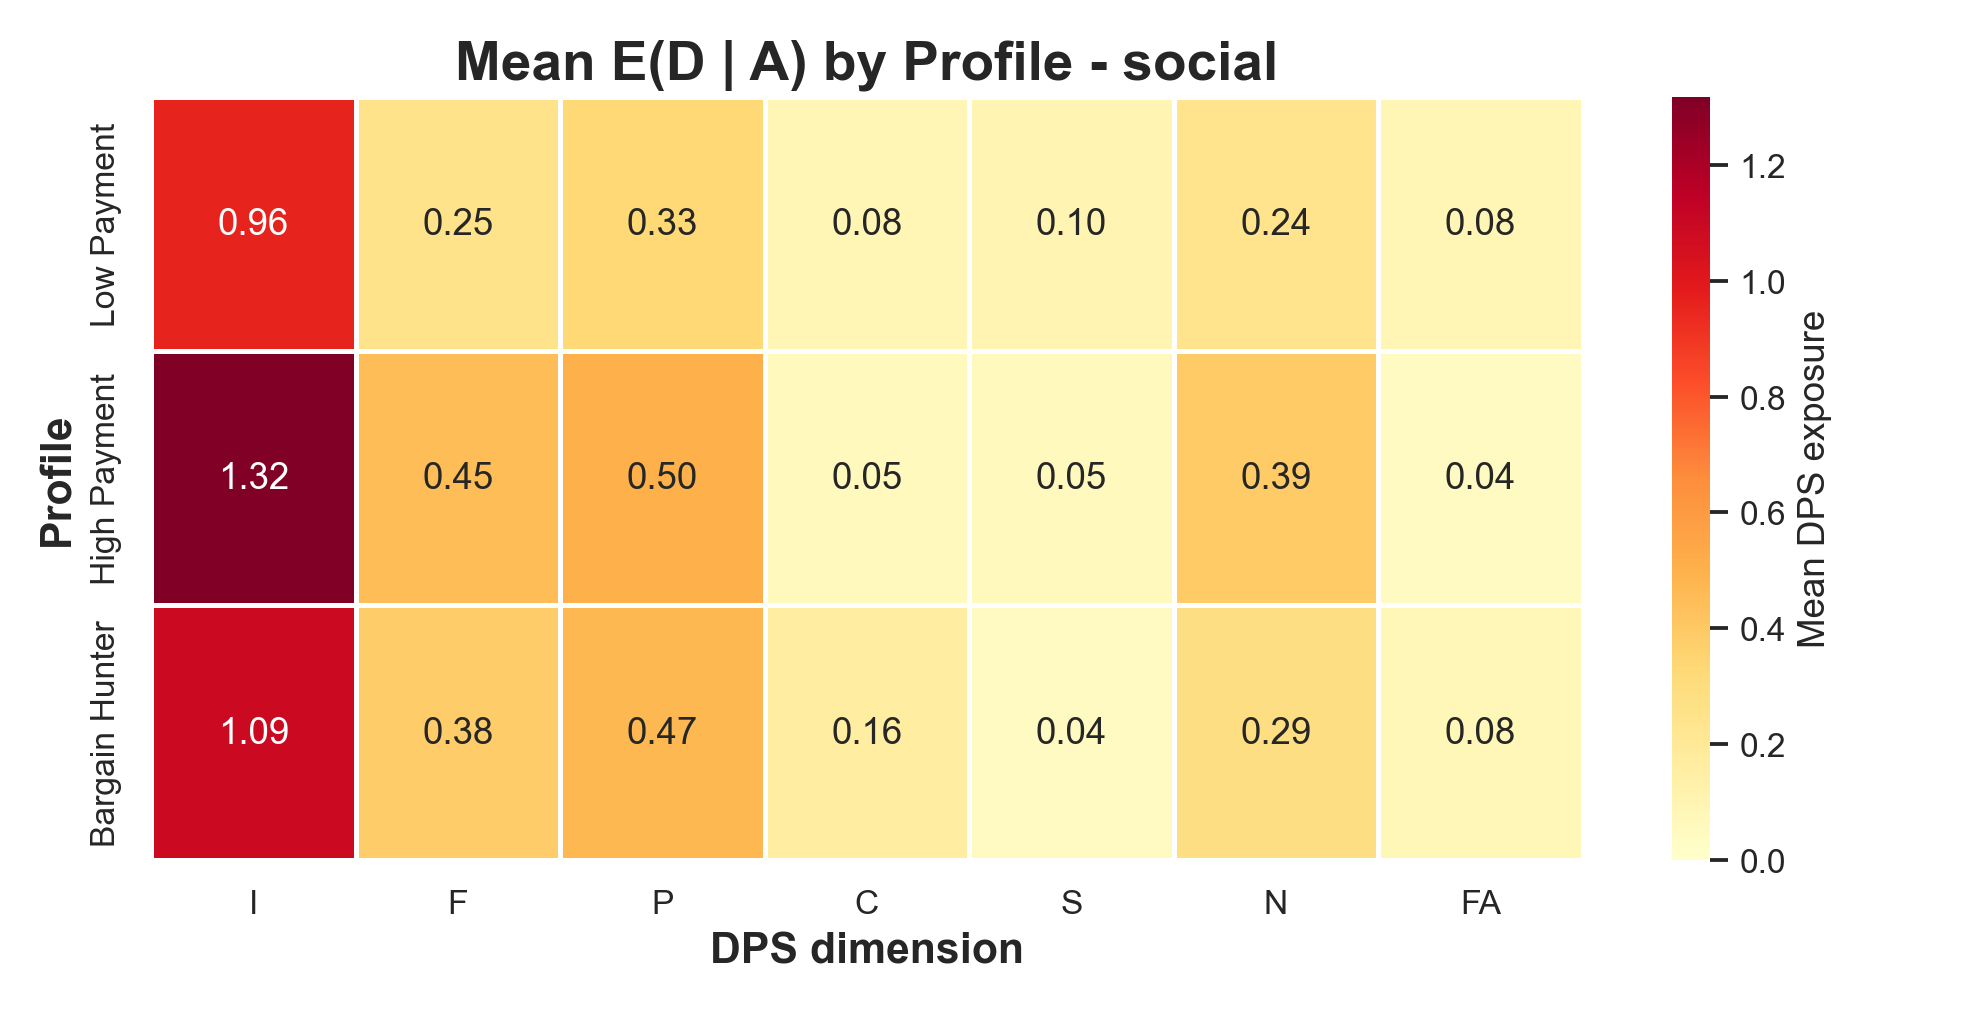
\includegraphics[width=0.95\linewidth]{figures/statistics/heatmap_mean_exposure_social.png}
    \caption{Mean DPS exposure heatmap for social applications.}
    \label{fig:mean-exposure-social}
\end{figure}

\paragraph{Interpretation.}
The profile-level means suggest observed exposure differences rather than a single universal dark-pattern profile for each app, but the averages alone are not sufficiently expressive. The high-payment shopping profile is associated with higher average exposure in Interface Interference and Pressure, which is consistent with trajectories that more often enter purchase, membership, shopping-cart, checkout, or promotion-related interfaces. The bargain-hunter profile also shows relatively high exposure in promotion-sensitive dimensions, which is consistent with searches for discounts, coupons, group-buying opportunities, flash sales, and reward mechanisms. By contrast, the low-payment browsing profile has the lowest aggregate mean, but it still encounters non-trivial Forced Action exposure, such as login, notification, location, or commitment prompts. More importantly, the food-delivery and social results, together with their heatmaps and category-level tables, make the exposure gap visibly clearer: the category-level patterns show a more pronounced separation between profiles than the global averages alone. These results suggest that dark pattern exposure is shaped by the interaction path followed by the user profile, not only by the static presence of interface elements in an app.

\paragraph{Caveat.}
These results should be interpreted as profile-conditioned exposure differences in the observed audit data. The experiment measures visible interface exposure under controlled profiles; it does not reveal the internal decision logic of the applications. Therefore, the findings are best understood as evidence that controlled profiles are associated with different DPS distributions. Whether these differences arise from personalization, rule-based interface flows, recommendation mechanisms, promotion systems, or ordinary navigation differences remains outside the scope of this experiment.

\section{Finding 2: Exposure Estimates Stabilize}

\paragraph{Result.}
The running mean convergence analysis suggests that the exposure estimates become more stable as interaction steps accumulate. Early trajectory segments fluctuate more strongly, while later segments move toward a narrower range. This pattern supports the use of repeated observations rather than isolated screenshots for estimating profile-conditioned exposure.

\paragraph{Evidence.}
For a given profile and DPS dimension, the running mean after step $t$ is calculated from all annotated observations collected from step 1 to step $t$. At the beginning of each exploration trajectory, a single pop-up, login prompt, checkout page, or promotional banner can strongly affect the cumulative average because the sample size is still small. After repeated interactions, the curves gradually become smoother. Most dimensions stabilize within the 20--30 step range used by the audit protocol, which indicates that the final profile-level estimates are less sensitive to any single screen state.

\paragraph{WangYiYun example.}
The WangYiYun trajectories provide a concrete illustration of this stabilization pattern at the single-application level. Figures~\ref{fig:wangyiyun-curve-high}, \ref{fig:wangyiyun-curve-low}, and \ref{fig:wangyiyun-curve-bargain} show the running mean exposure curves for the high-payment shopping, low-payment browsing, and bargain-hunter profiles, respectively. Although the early steps fluctuate more strongly, the later segments become visibly smoother, especially for the dominant dimensions that remain active across repeated interactions.

\begin{figure}[htbp]
    \centering
    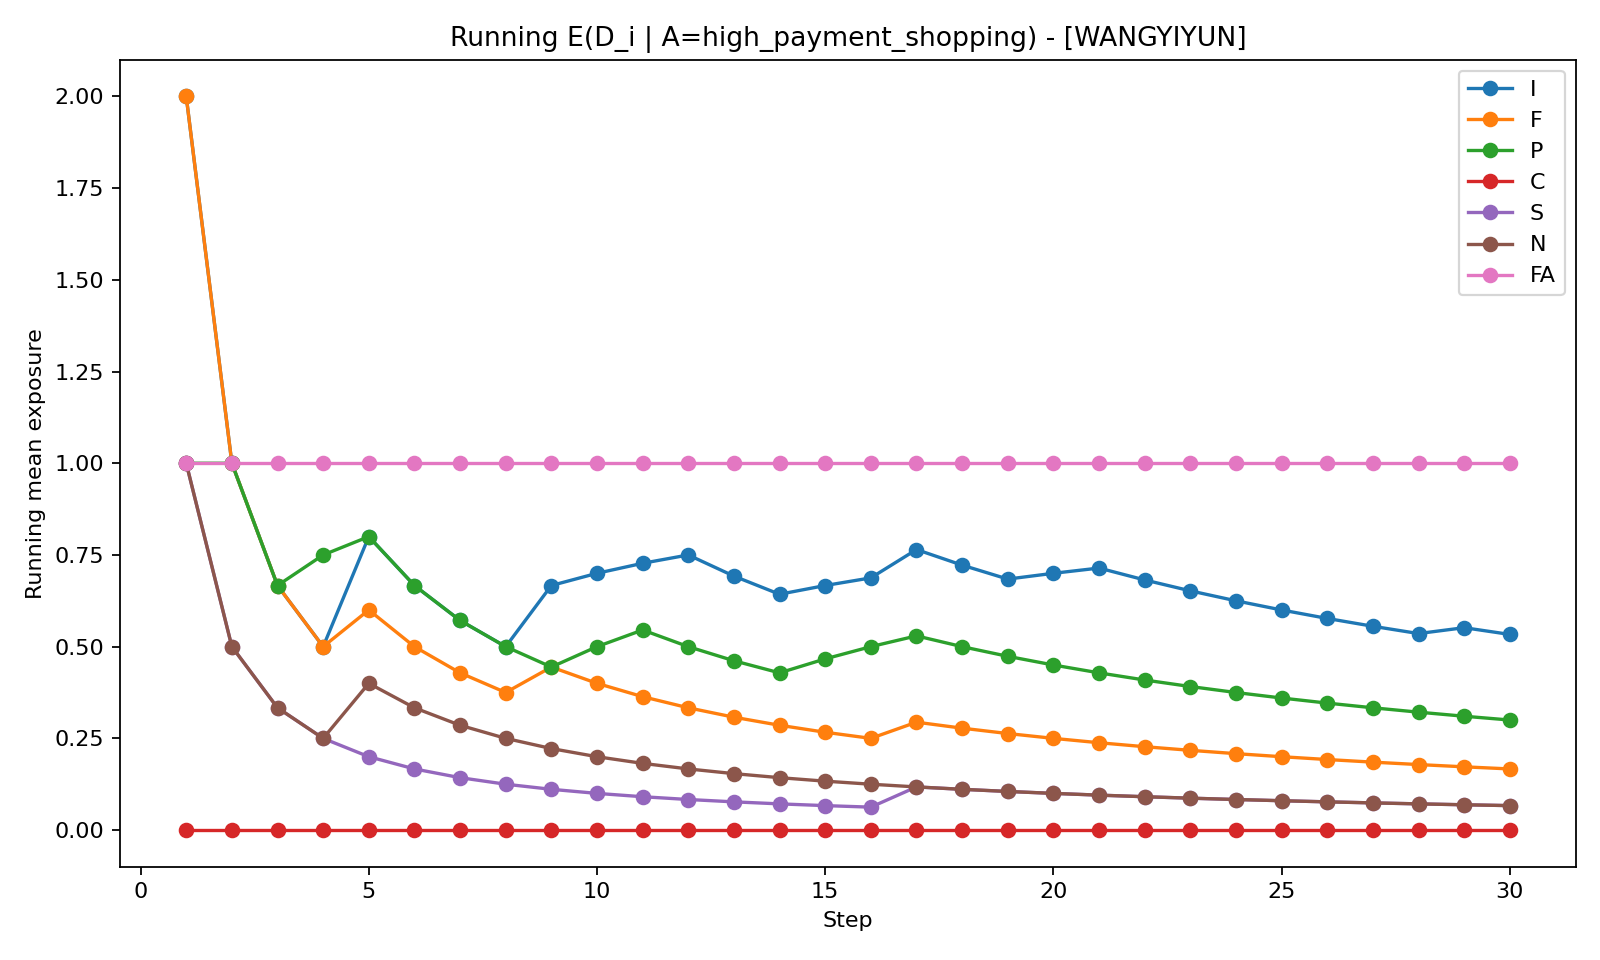
\includegraphics[width=0.85\linewidth]{figures/statistics/curves_entertainment/curve_E_high_payment_shopping_WangYiYun_entertainment.png}
    \caption{Running mean DPS exposure curve for WangYiYun under the high-payment shopping profile.}
    \label{fig:wangyiyun-curve-high}
\end{figure}

\begin{figure}[htbp]
    \centering
    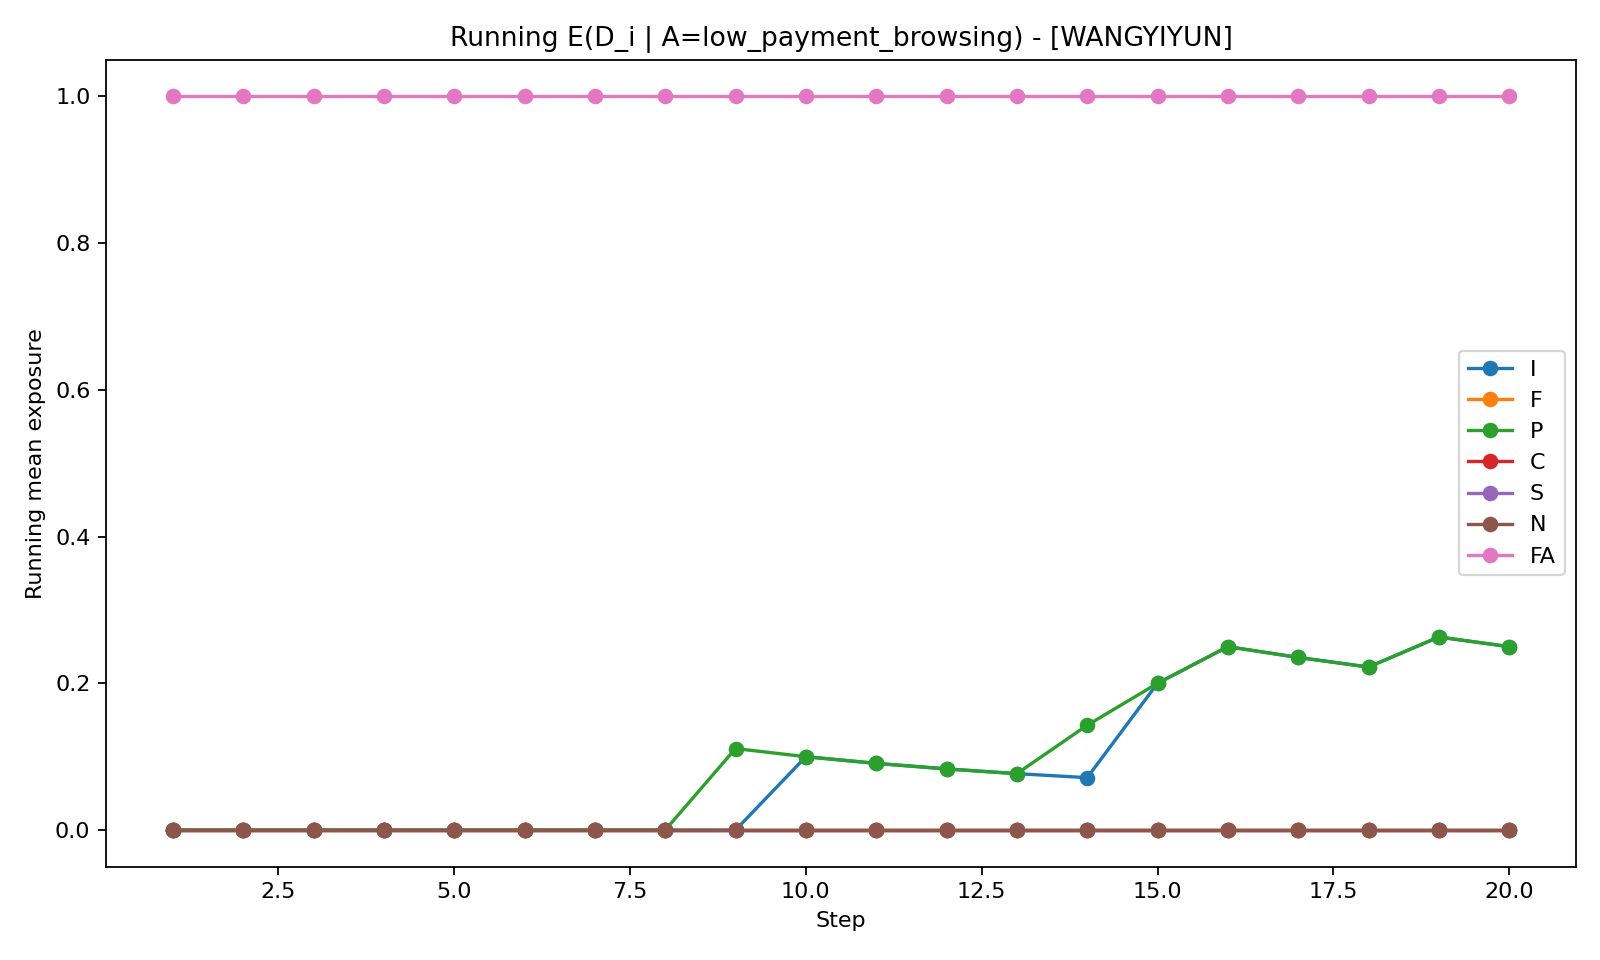
\includegraphics[width=0.85\linewidth]{figures/statistics/curves_entertainment/curve_E_low_payment_browsing_WangYiYun_entertainment.png}
    \caption{Running mean DPS exposure curve for WangYiYun under the low-payment browsing profile.}
    \label{fig:wangyiyun-curve-low}
\end{figure}

\begin{figure}[htbp]
    \centering
    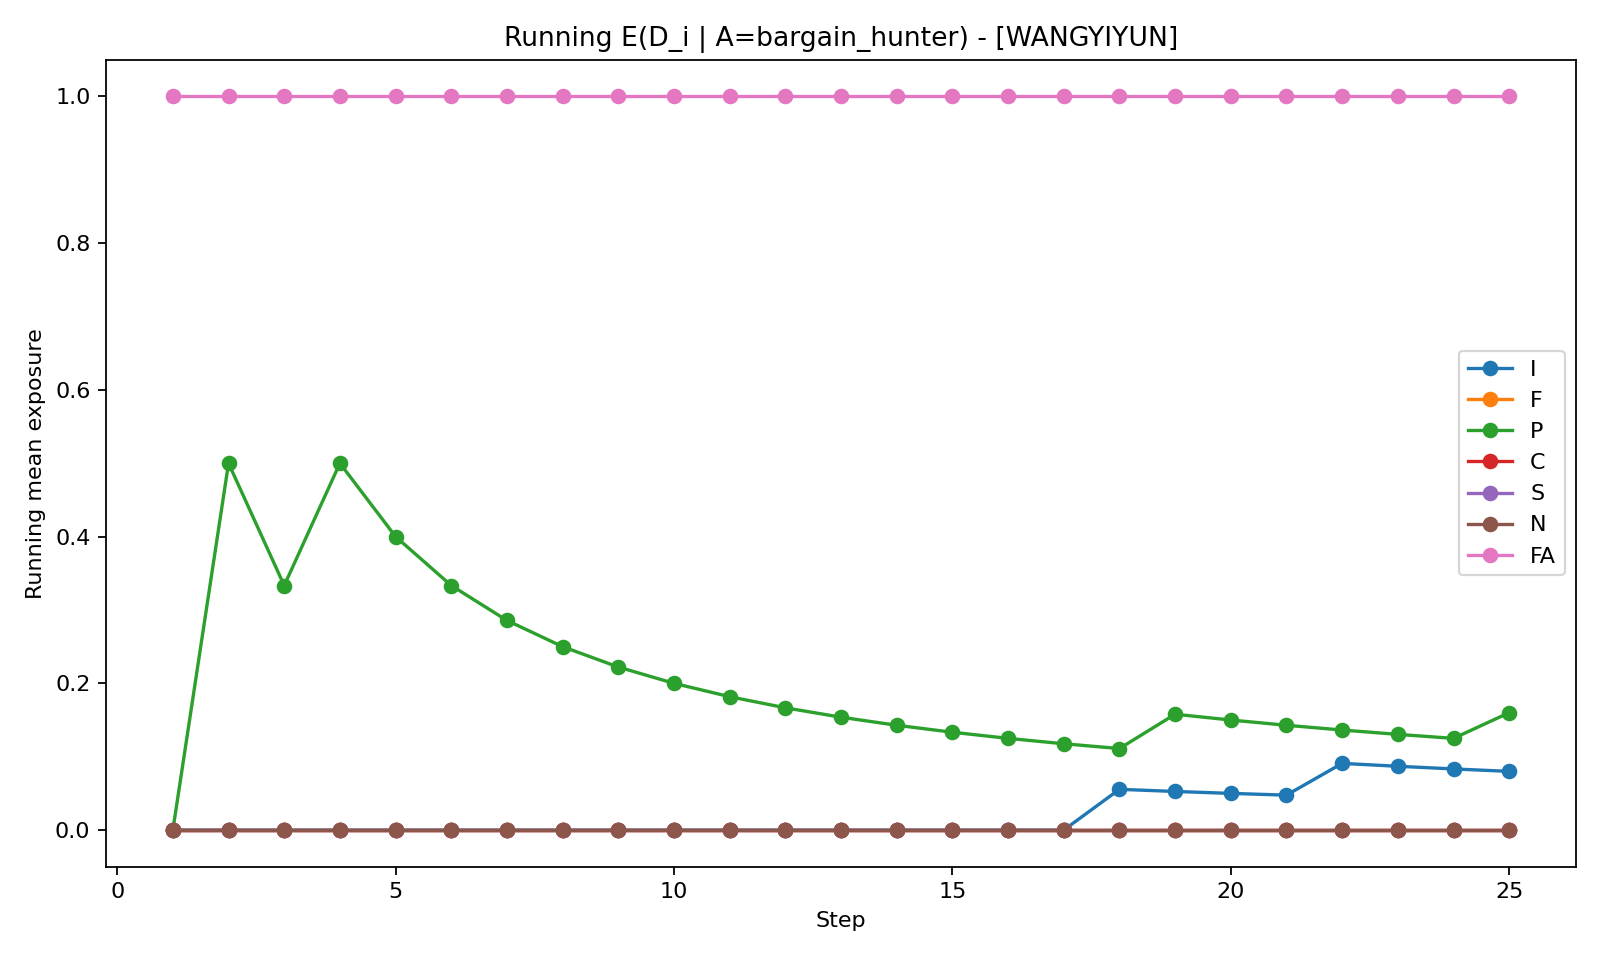
\includegraphics[width=0.85\linewidth]{figures/statistics/curves_entertainment/curve_E_bargain_hunter_WangYiYun_entertainment.png}
    \caption{Running mean DPS exposure curve for WangYiYun under the bargain-hunter profile.}
    \label{fig:wangyiyun-curve-bargain}
\end{figure}

\paragraph{Interpretation.}
The convergence pattern supports the methodological choice of treating exposure as an expectation, denoted as $E(D \mid A)$, rather than as a simple count of detected dark pattern instances. A count-based measure can show how many times a label appears, but it does not directly express the average exposure level associated with a profile-conditioned trajectory. The running mean curves make this expectation-based interpretation visible. As the trajectory grows longer, the estimate becomes less sensitive to individual screens and more representative of the profile's typical exposure pattern in that app or category. This design follows the broader logic of algorithm auditing and exposure measurement, where repeated observations are needed to characterize the behavior of black-box systems under controlled conditions \cite{sandvig2014auditing,hannak2013personalization,srba2023youtube}.

\paragraph{Caveat.}
Stabilization within the audited trajectories does not mean that all possible dark pattern exposure in an application has been exhausted. Some dark patterns may appear only after longer-term use, repeated purchases, account aging, seasonal promotions, or accumulated behavioral history. In addition, the archived result files show that a small number of app-profile runs contain fewer than the planned 30 steps. The convergence result therefore supports the reliability of this course-scale experiment, but it does not remove the need for longer-term or larger-scale audits.

\section{Finding 3: Statistical Evidence for Profile-dependent Exposure}

\begin{figure}[htbp]
    \centering
    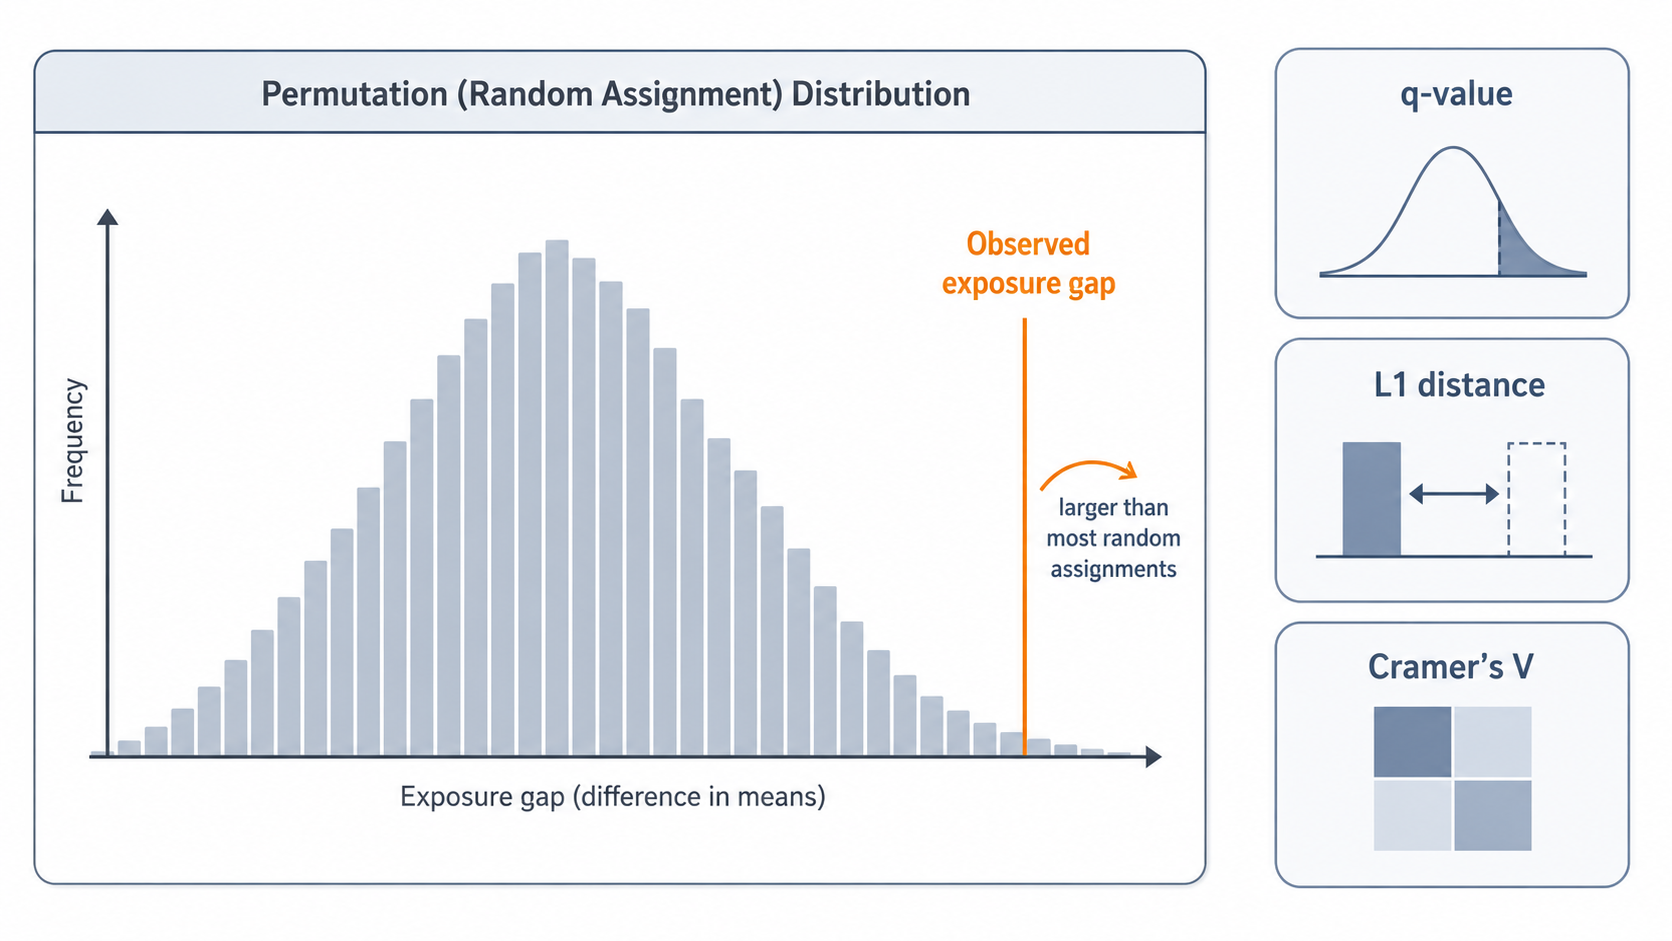
\includegraphics[width=0.95\linewidth]{figures/pictures/permutation_test_intuition.png}
    \caption{Permutation Test Intuition}
    \label{fig:permutation_test_intuition}
\end{figure}

\paragraph{Result.}
The statistical tests provide mixed but informative evidence for profile-dependent exposure. Across all apps, the low-payment browsing and high-payment shopping profiles differ significantly after false-discovery-rate correction. At the category level, the strongest evidence appears in eating and social applications, while the entertainment category does not show statistically robust pairwise differences under the permutation tests.

\begin{table}[htbp]
    \centering
    \caption{Statistical summary of profile-dependent DPS exposure differences.}
    \label{tab:statistical-summary}
    \footnotesize
    \setlength{\tabcolsep}{4pt}
    \renewcommand{\arraystretch}{1.08}
    \begin{tabular}{@{}p{0.26\linewidth}p{0.09\linewidth}p{0.08\linewidth}p{0.08\linewidth}p{0.08\linewidth}p{0.08\linewidth}p{0.28\linewidth}@{}}
        \toprule
        Comparison & Scope & $p$-value & $q$-value & L1 distance & Cramér's $V$ & Interpretation \\
        \midrule
        Low browsing vs. High shopping & All & 0.0082 & 0.0246 & 0.301 & 0.050 & FDR-significant difference \\
        Low browsing vs. Bargain hunter & All & 0.0832 & 0.1248 & 0.227 & 0.078 & Not statistically robust \\
        High shopping vs. Bargain hunter & All & 0.3633 & 0.3633 & 0.164 & 0.061 & Not statistically robust \\
        Low browsing vs. High shopping & Eating & 0.0018 & 0.0054 & 0.542 & 0.129 & FDR-significant difference \\
        Low browsing vs. Bargain hunter & Eating & 0.0072 & 0.0108 & 0.467 & 0.155 & FDR-significant difference \\
        High shopping vs. Bargain hunter & Eating & 0.1776 & 0.1776 & 0.292 & 0.134 & Not statistically robust \\
        Low browsing vs. High shopping & Entertainment & 0.8386 & 0.8644 & 0.187 & 0.159 & Not statistically robust \\
        Low browsing vs. Bargain hunter & Entertainment & 0.5505 & 0.8644 & 0.269 & 0.156 & Not statistically robust \\
        High shopping vs. Bargain hunter & Entertainment & 0.8644 & 0.8644 & 0.186 & 0.047 & Not statistically robust \\
        Low browsing vs. High shopping & Shopping & 0.0784 & 0.1176 & 0.200 & 0.100 & Not statistically robust \\
        Low browsing vs. Bargain hunter & Shopping & 0.2759 & 0.2759 & 0.175 & 0.113 & Not statistically robust \\
        High shopping vs. Bargain hunter & Shopping & 0.0058 & 0.0174 & 0.325 & 0.180 & FDR-significant difference \\
        Low browsing vs. High shopping & Social & 0.0002 & 0.0006 & 0.997 & 0.155 & FDR-significant difference \\
        Low browsing vs. Bargain hunter & Social & 0.0400 & 0.0400 & 0.585 & 0.125 & FDR-significant difference \\
        High shopping vs. Bargain hunter & Social & 0.0388 & 0.0400 & 0.584 & 0.149 & FDR-significant difference \\
        \bottomrule
    \end{tabular}
\end{table}

\paragraph{Evidence.}
Figures~\ref{fig:mannwhitney-qvalue-all}, \ref{fig:permutation-pvalues}, \ref{fig:permutation-l1}, and \ref{fig:cramers-v} report the statistical validation results used to evaluate profile-dependent exposure differences. Table~\ref{tab:statistical-summary} summarizes the numerical results from the repository's statistical-test CSV files. The first figure is a dimension-level Mann-Whitney U BH FDR q-value heatmap, whereas the permutation figures summarize profile-label randomization at the profile-comparison scope. The permutation tests evaluate whether observed exposure gaps are larger than what would be expected under random profile assignment. The q-values adjust significance interpretation across multiple comparisons using Benjamini-Hochberg FDR correction. The L1 distance measures the practical magnitude of differences between DPS exposure vectors. Cramér's V measures the association strength between profile type and DPS exposure.

\begin{figure}[htbp]
    \centering
    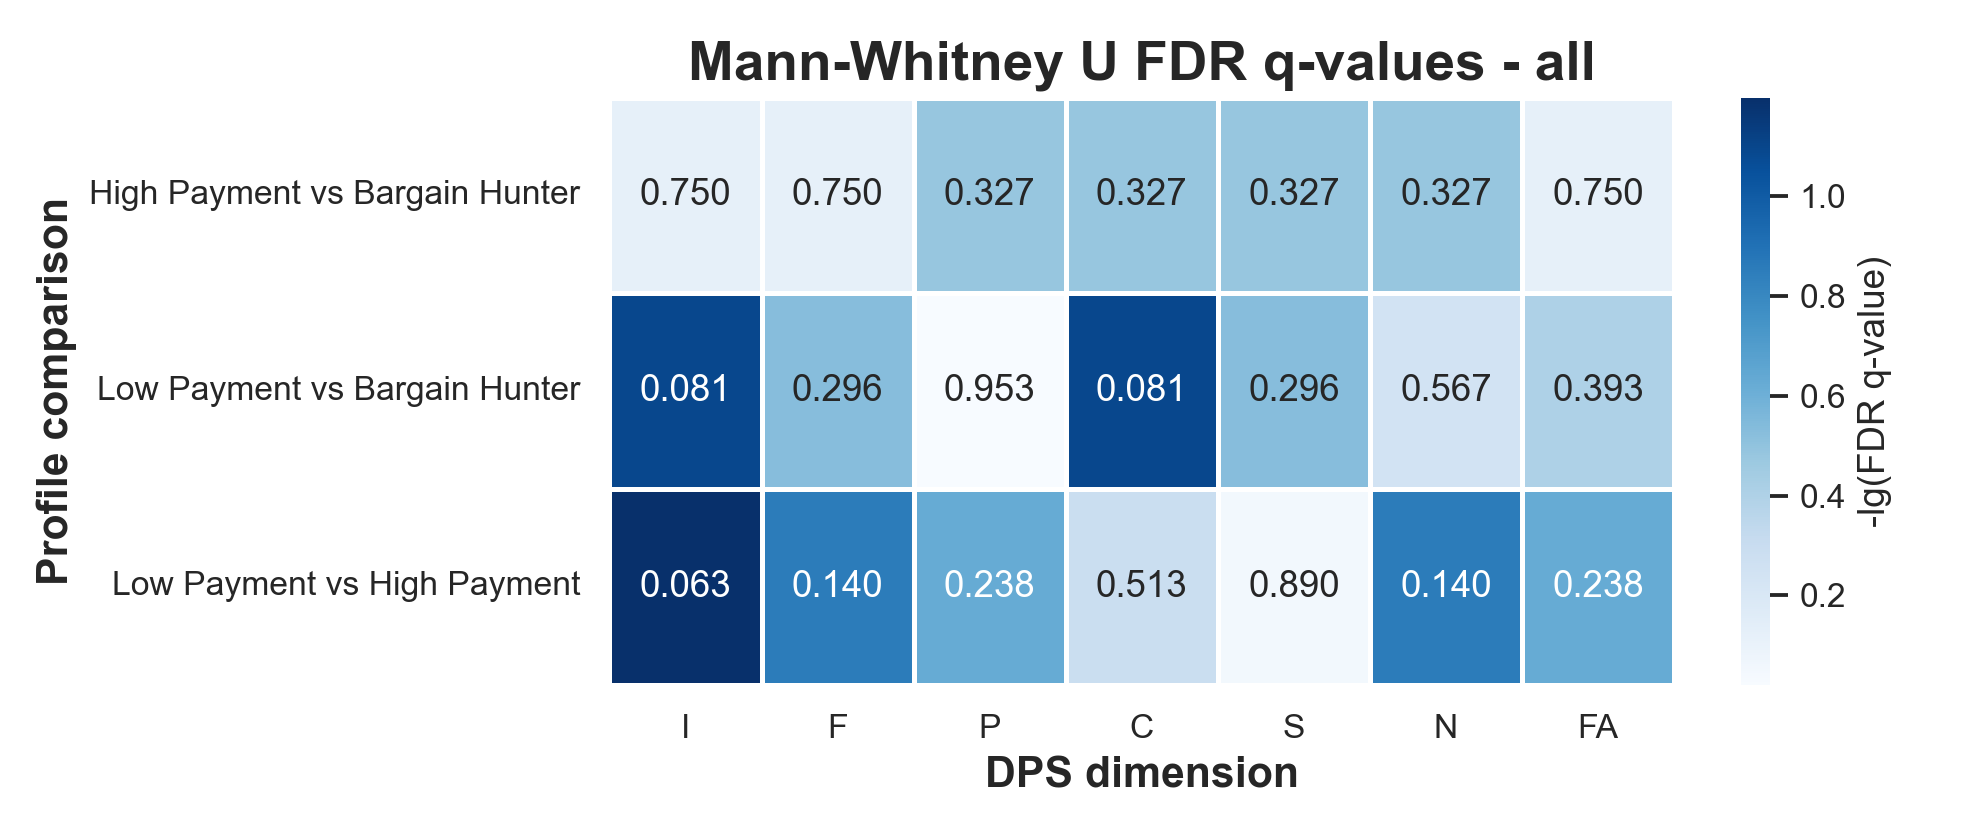
\includegraphics[width=0.95\linewidth]{figures/statistics/mannwhitney_qvalue_heatmap_all.png}
    \caption{Mann-Whitney U BH FDR q-value heatmap for dimension-level DPS exposure comparisons across all audited applications.}
    \label{fig:mannwhitney-qvalue-all}
\end{figure}

\begin{figure}[htbp]
    \centering
    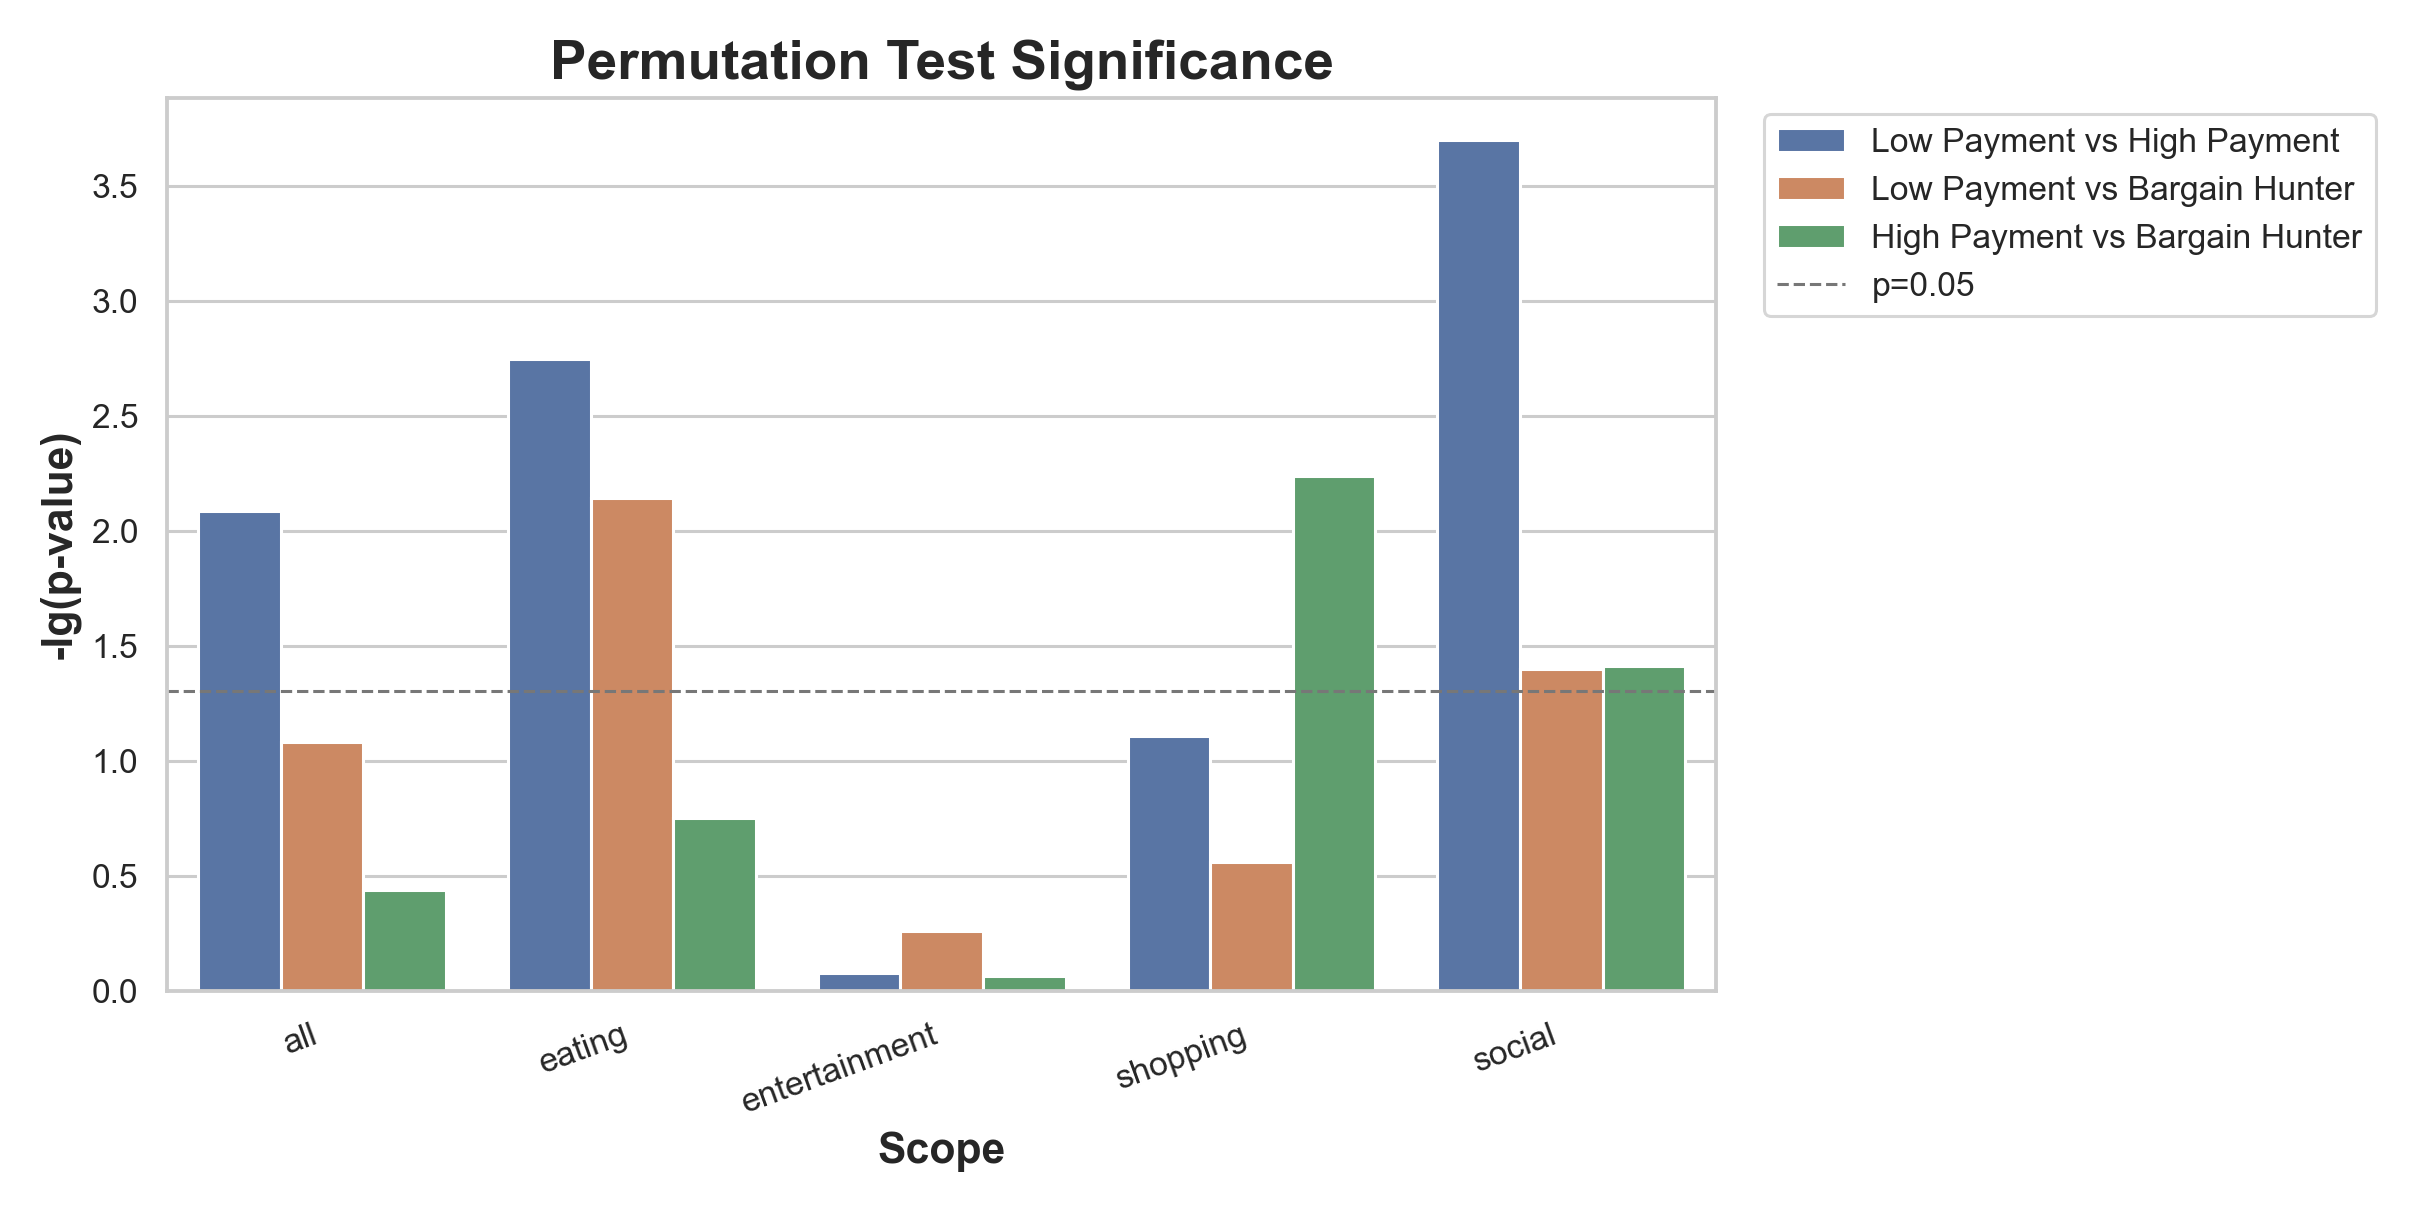
\includegraphics[width=0.95\linewidth]{figures/statistics/permutation_pvalues_by_scope.png}
    \caption{Permutation-test p-values by comparison scope.}
    \label{fig:permutation-pvalues}
\end{figure}

\begin{figure}[htbp]
    \centering
    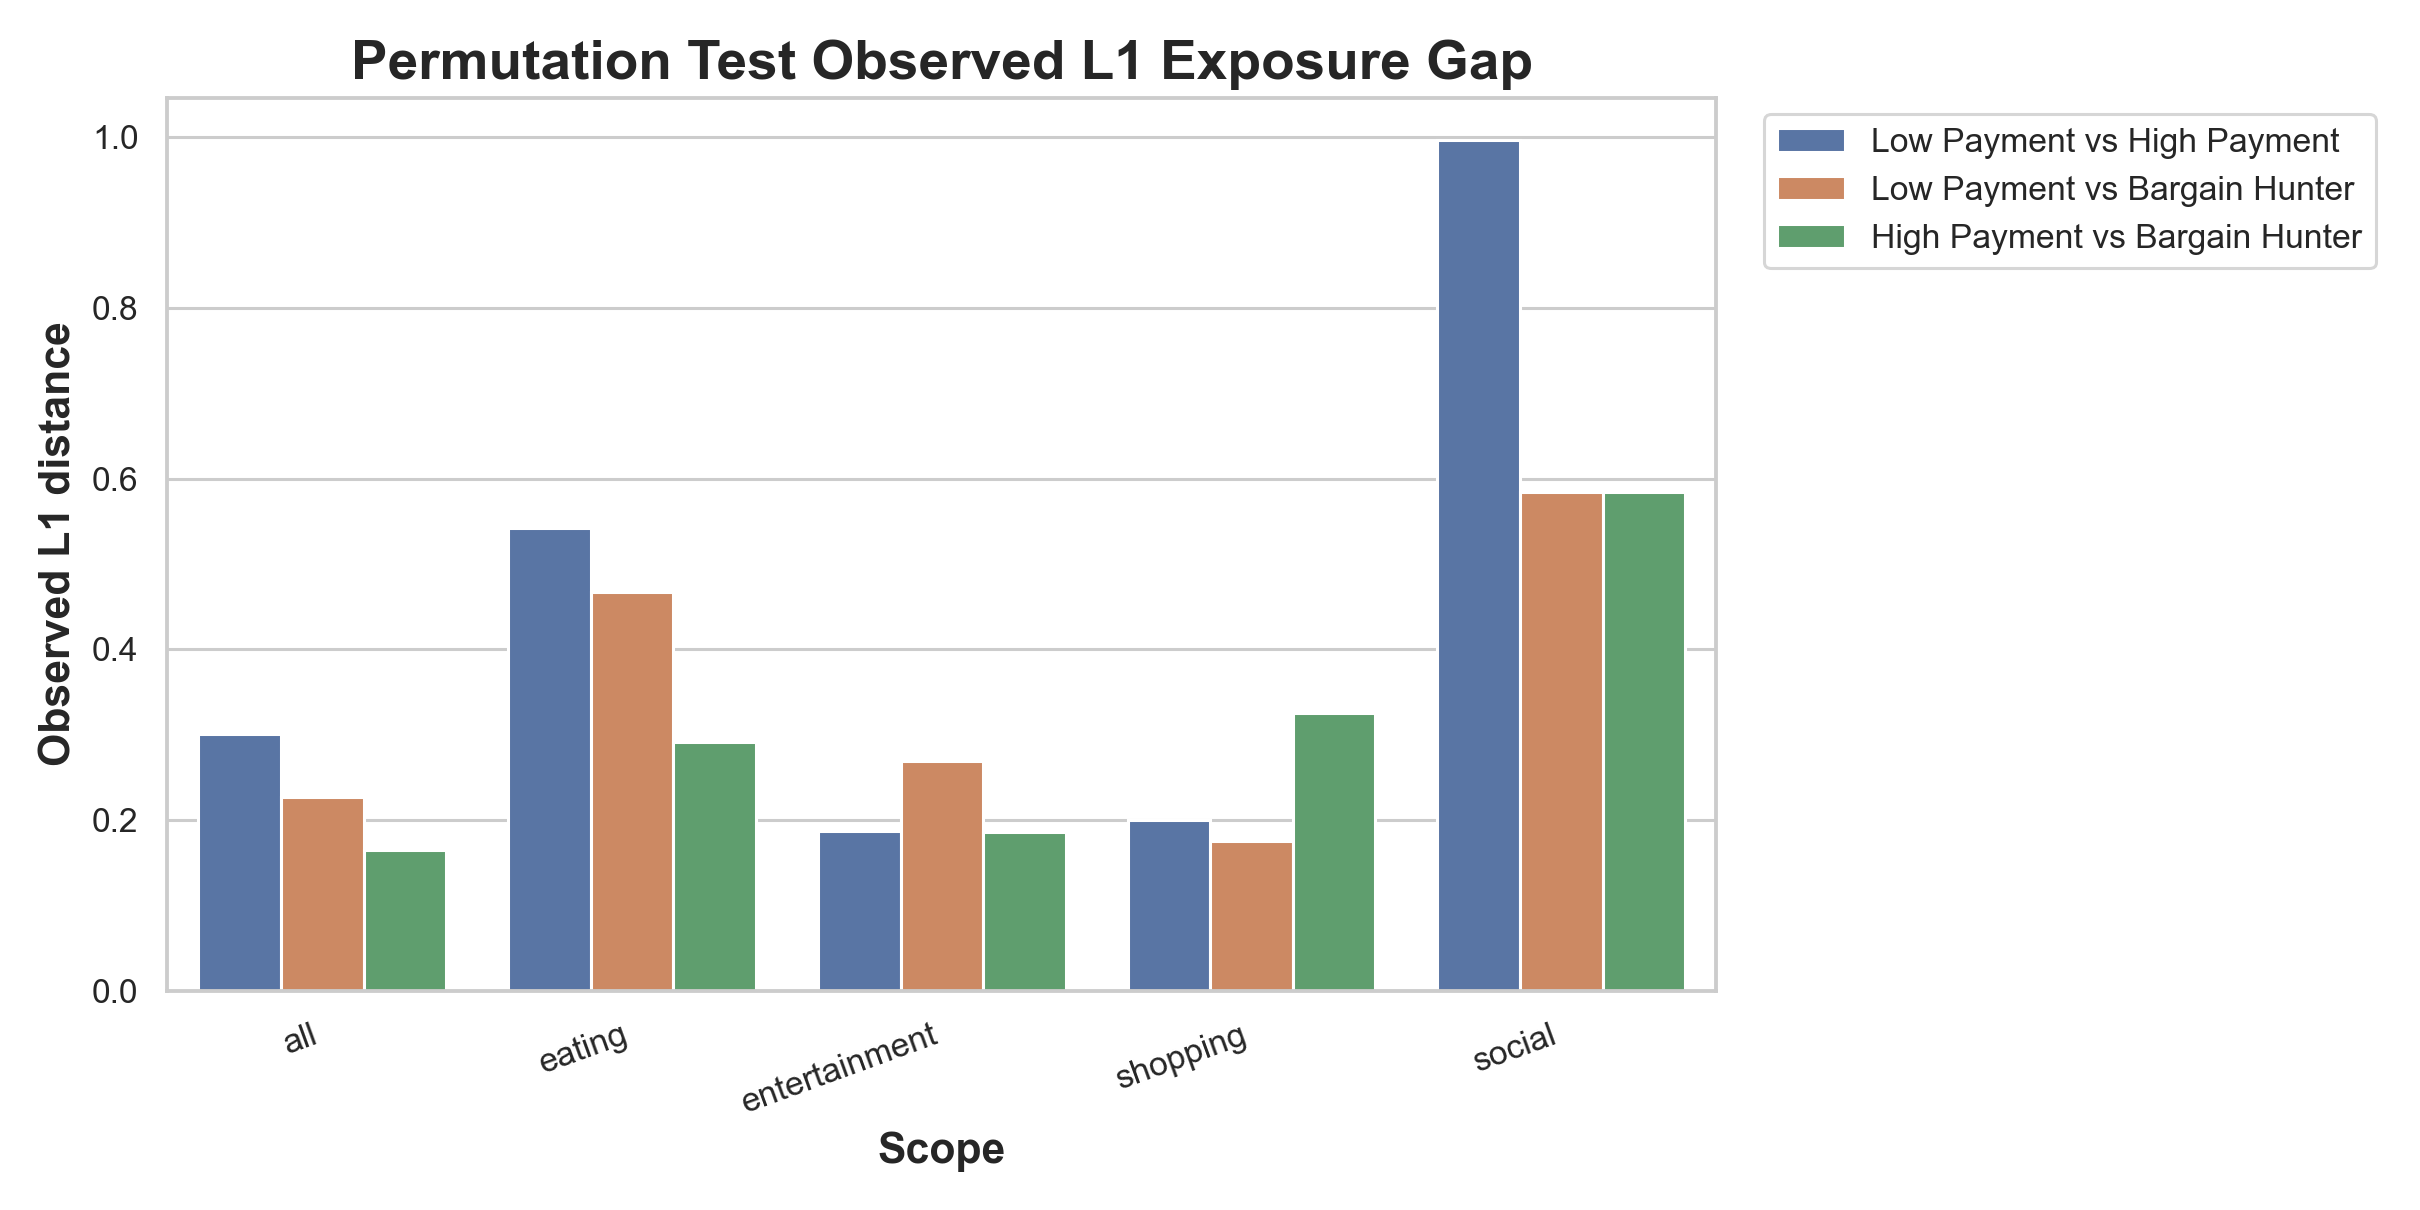
\includegraphics[width=0.95\linewidth]{figures/statistics/permutation_observed_l1_by_scope.png}
    \caption{Observed L1 exposure distances by comparison scope.}
    \label{fig:permutation-l1}
\end{figure}

\begin{figure}[htbp]
    \centering
    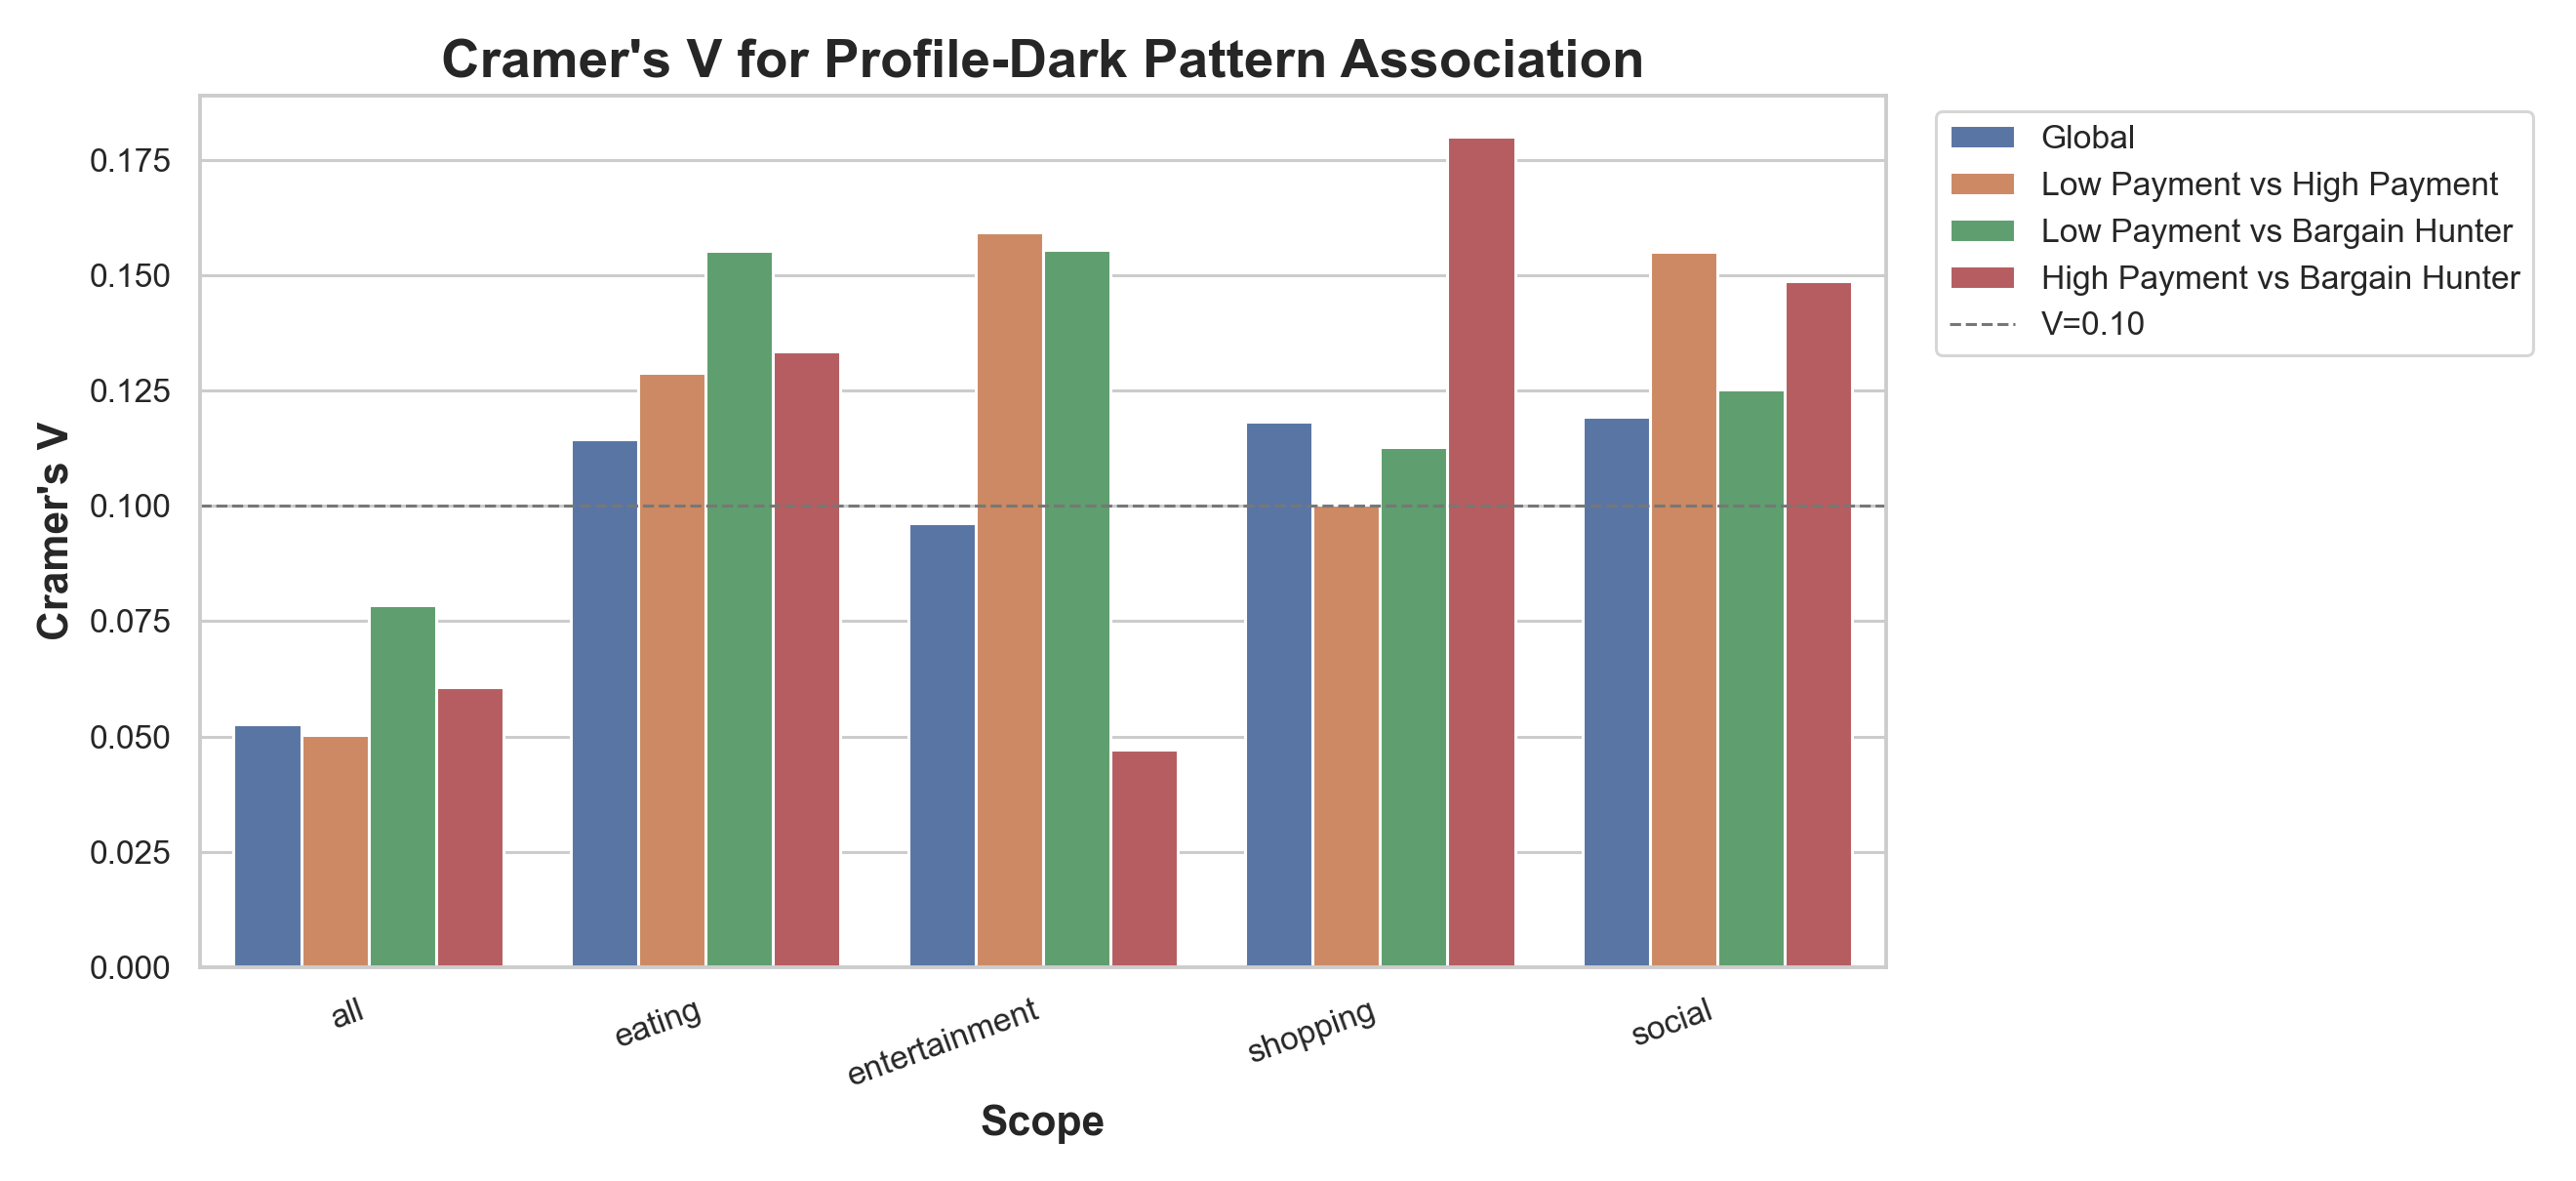
\includegraphics[width=0.95\linewidth]{figures/statistics/cramers_v_by_scope.png}
    \caption{Cramér's \(V\) association strength by comparison scope.}
    \label{fig:cramers-v}
\end{figure}

\paragraph{Interpretation.}
The all-app comparison suggests that low-payment browsing and high-payment shopping are associated with different exposure distributions. The category-level results further show that observed exposure differences are not evenly distributed across app domains. Eating and social applications show several FDR-significant pairwise comparisons, and shopping applications show a significant difference between high-payment shopping and bargain-hunter profiles. Entertainment applications, by contrast, do not show statistically robust pairwise differences in the current result files. The L1 distances help distinguish practical exposure gaps from purely statistical effects, while Cramér's V indicates that the observed associations are generally small to modest.

\paragraph{Caveat.}
The statistical evidence should be interpreted as association, not as evidence about internal app mechanisms. The permutation tests depend on the observed audit sample, the q-values depend on the chosen family of comparisons, and Cramér's V is computed from binary contingency summaries built from DPS presence versus absence. These metrics therefore strengthen the claim that observed exposure differences exist in the audited data, but they do not identify whether those differences come from personalization, recommendation flows, promotion modules, permissions, login gates, or ordinary navigation paths.

\section{Category-level Observations}

Beyond profile-level differences, the results also reveal several category-level patterns. These observations should be interpreted as empirical patterns from the audited applications and as plausible interpretations of interface mechanisms, rather than universal claims about all applications in a category. Figures~\ref{fig:category-heatmap-shopping}, \ref{fig:category-heatmap-eating}, \ref{fig:category-heatmap-entertainment}, and \ref{fig:category-heatmap-social} summarize category-level exposure patterns.

\begin{figure}[htbp]
    \centering
    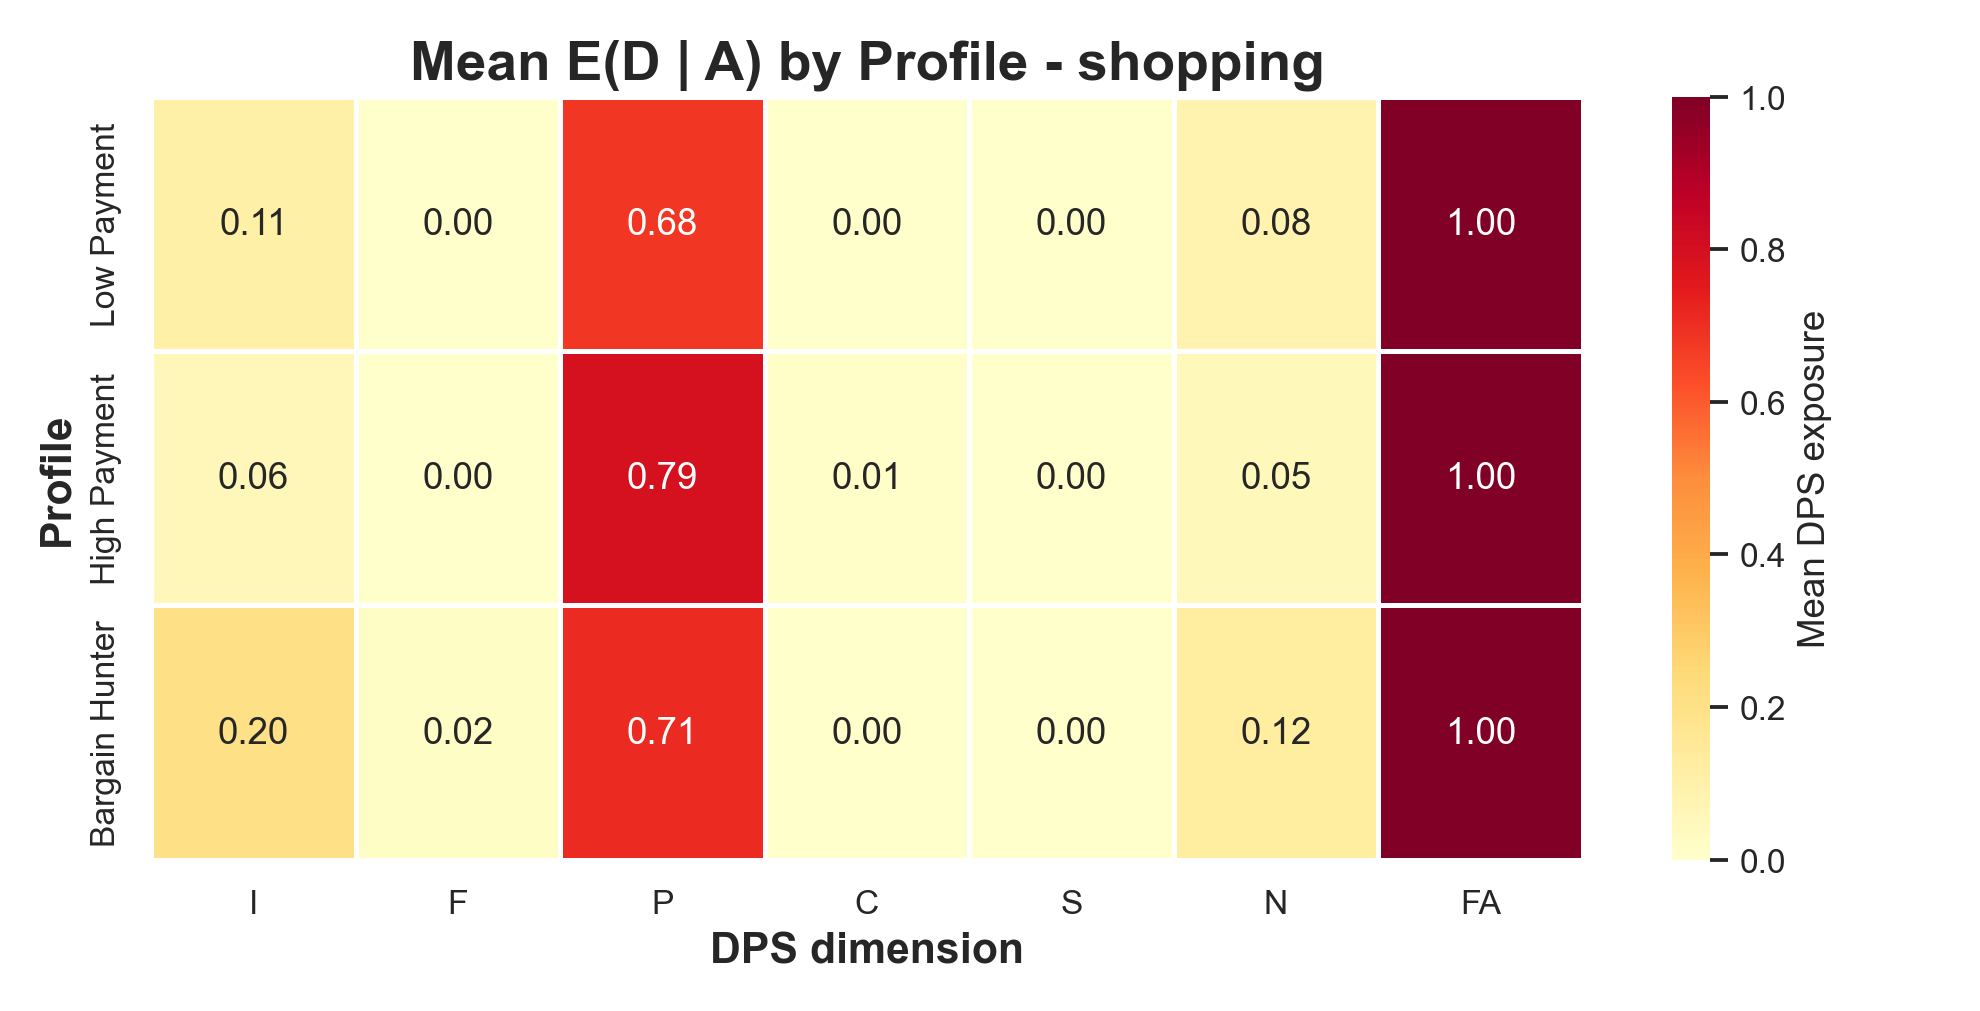
\includegraphics[width=0.95\linewidth]{figures/statistics/heatmap_mean_exposure_shopping.png}
    \caption{Mean DPS exposure heatmap for shopping applications.}
    \label{fig:category-heatmap-shopping}
\end{figure}

\begin{figure}[htbp]
    \centering
    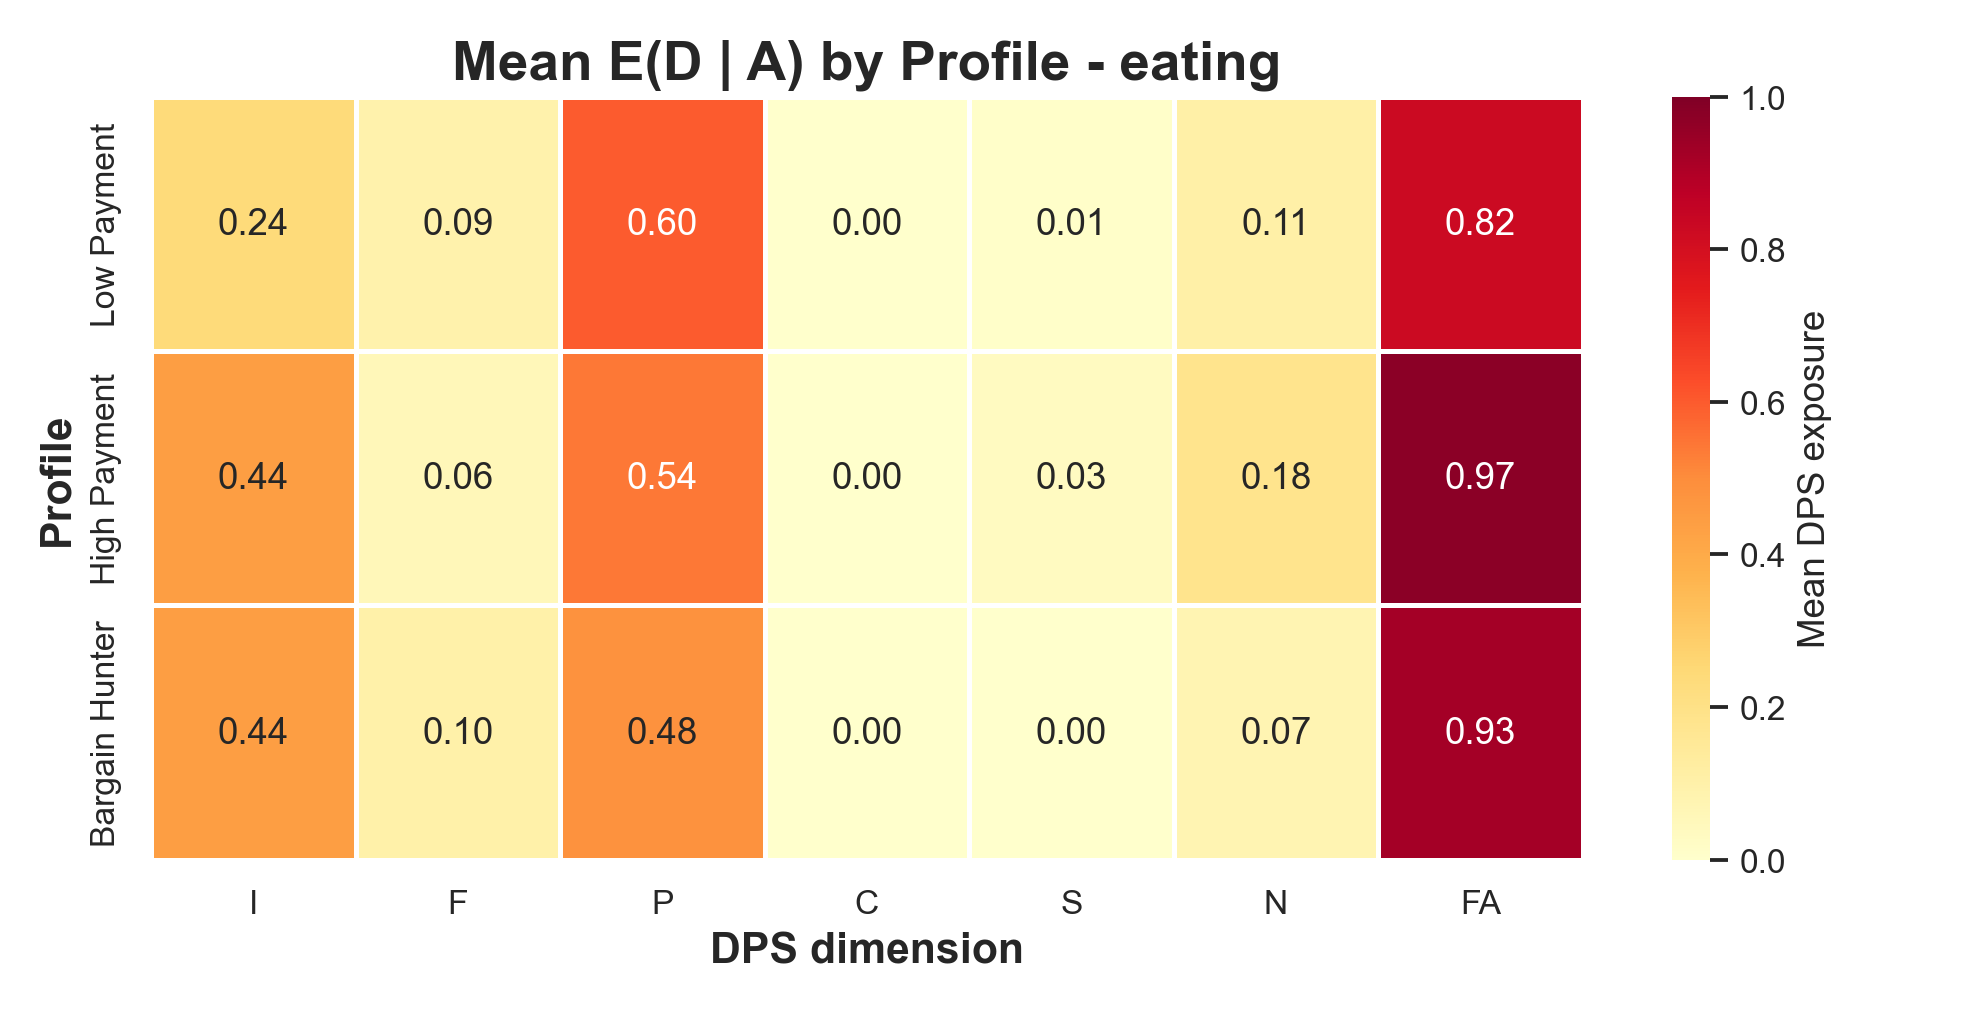
\includegraphics[width=0.95\linewidth]{figures/statistics/heatmap_mean_exposure_eating.png}
    \caption{Mean DPS exposure heatmap for food-delivery and eating-related applications.}
    \label{fig:category-heatmap-eating}
\end{figure}

\begin{figure}[htbp]
    \centering
    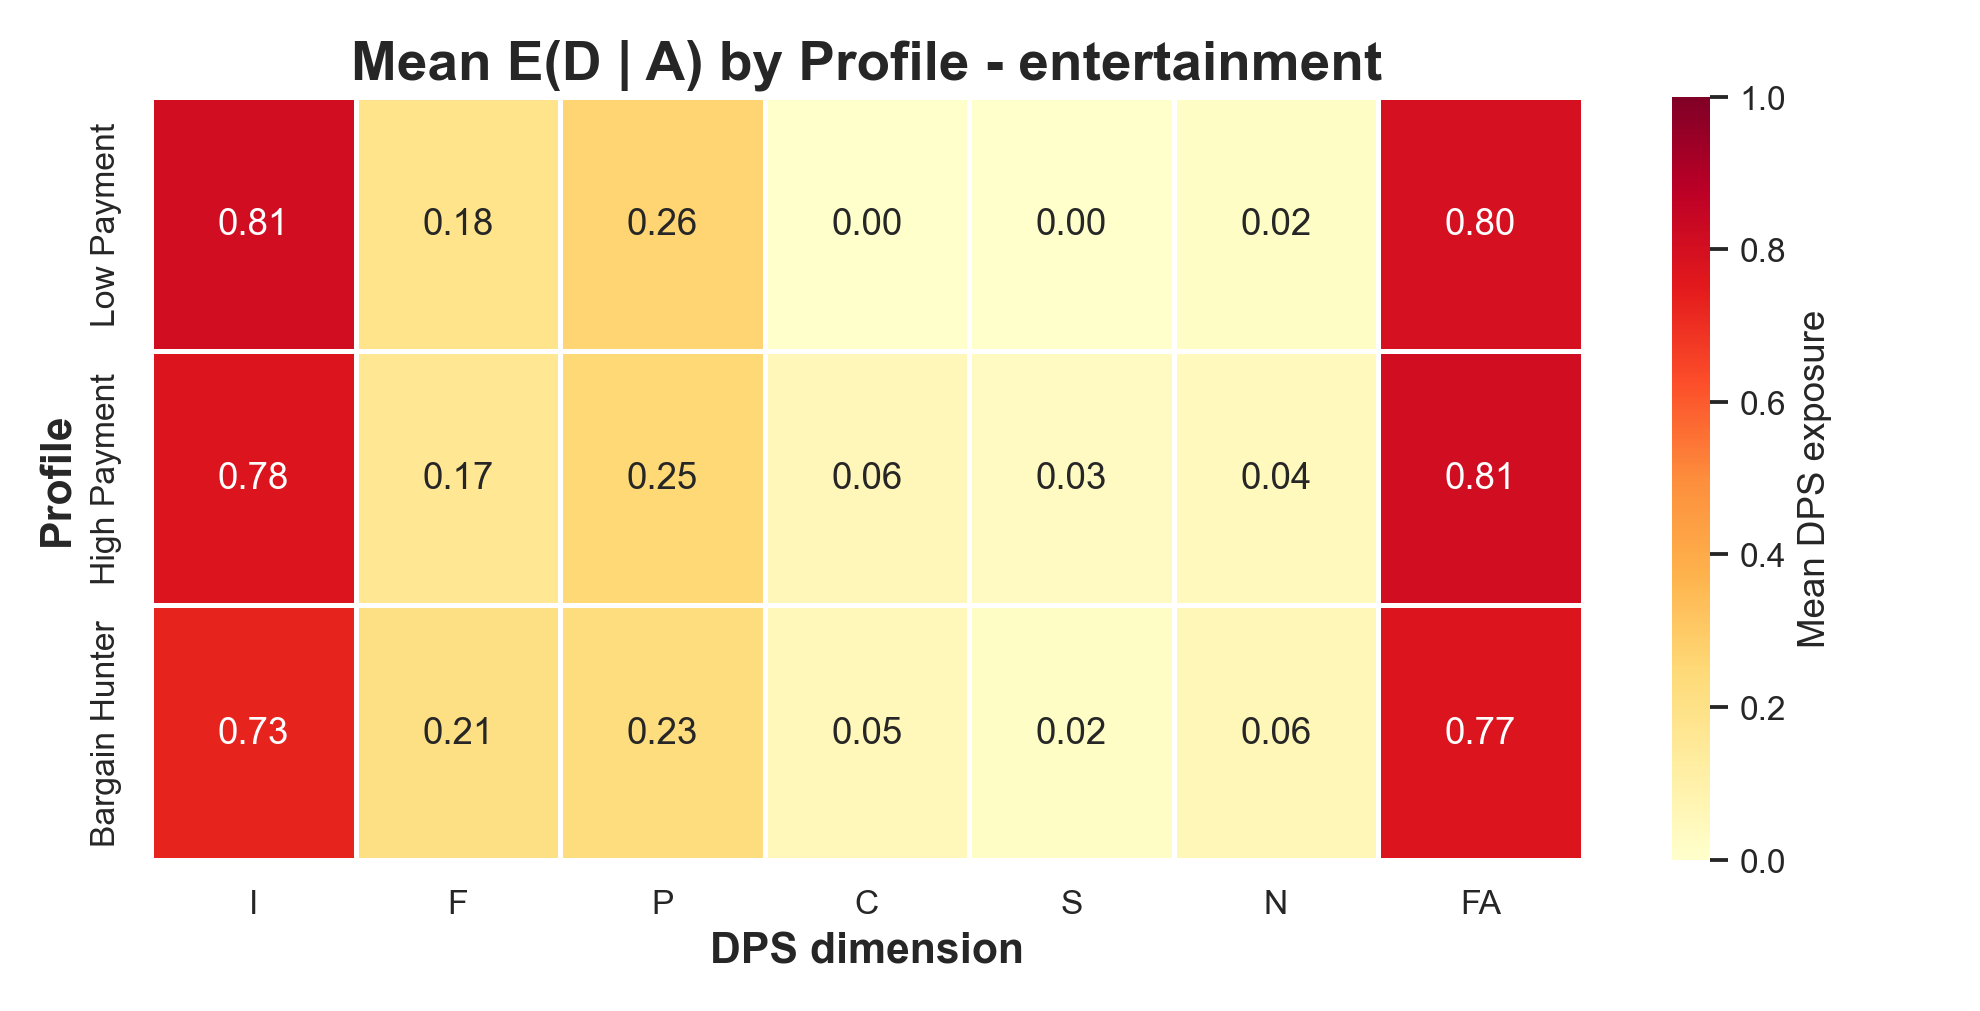
\includegraphics[width=0.95\linewidth]{figures/statistics/heatmap_mean_exposure_entertainment.png}
    \caption{Mean DPS exposure heatmap for entertainment applications.}
    \label{fig:category-heatmap-entertainment}
\end{figure}

\begin{figure}[htbp]
    \centering
    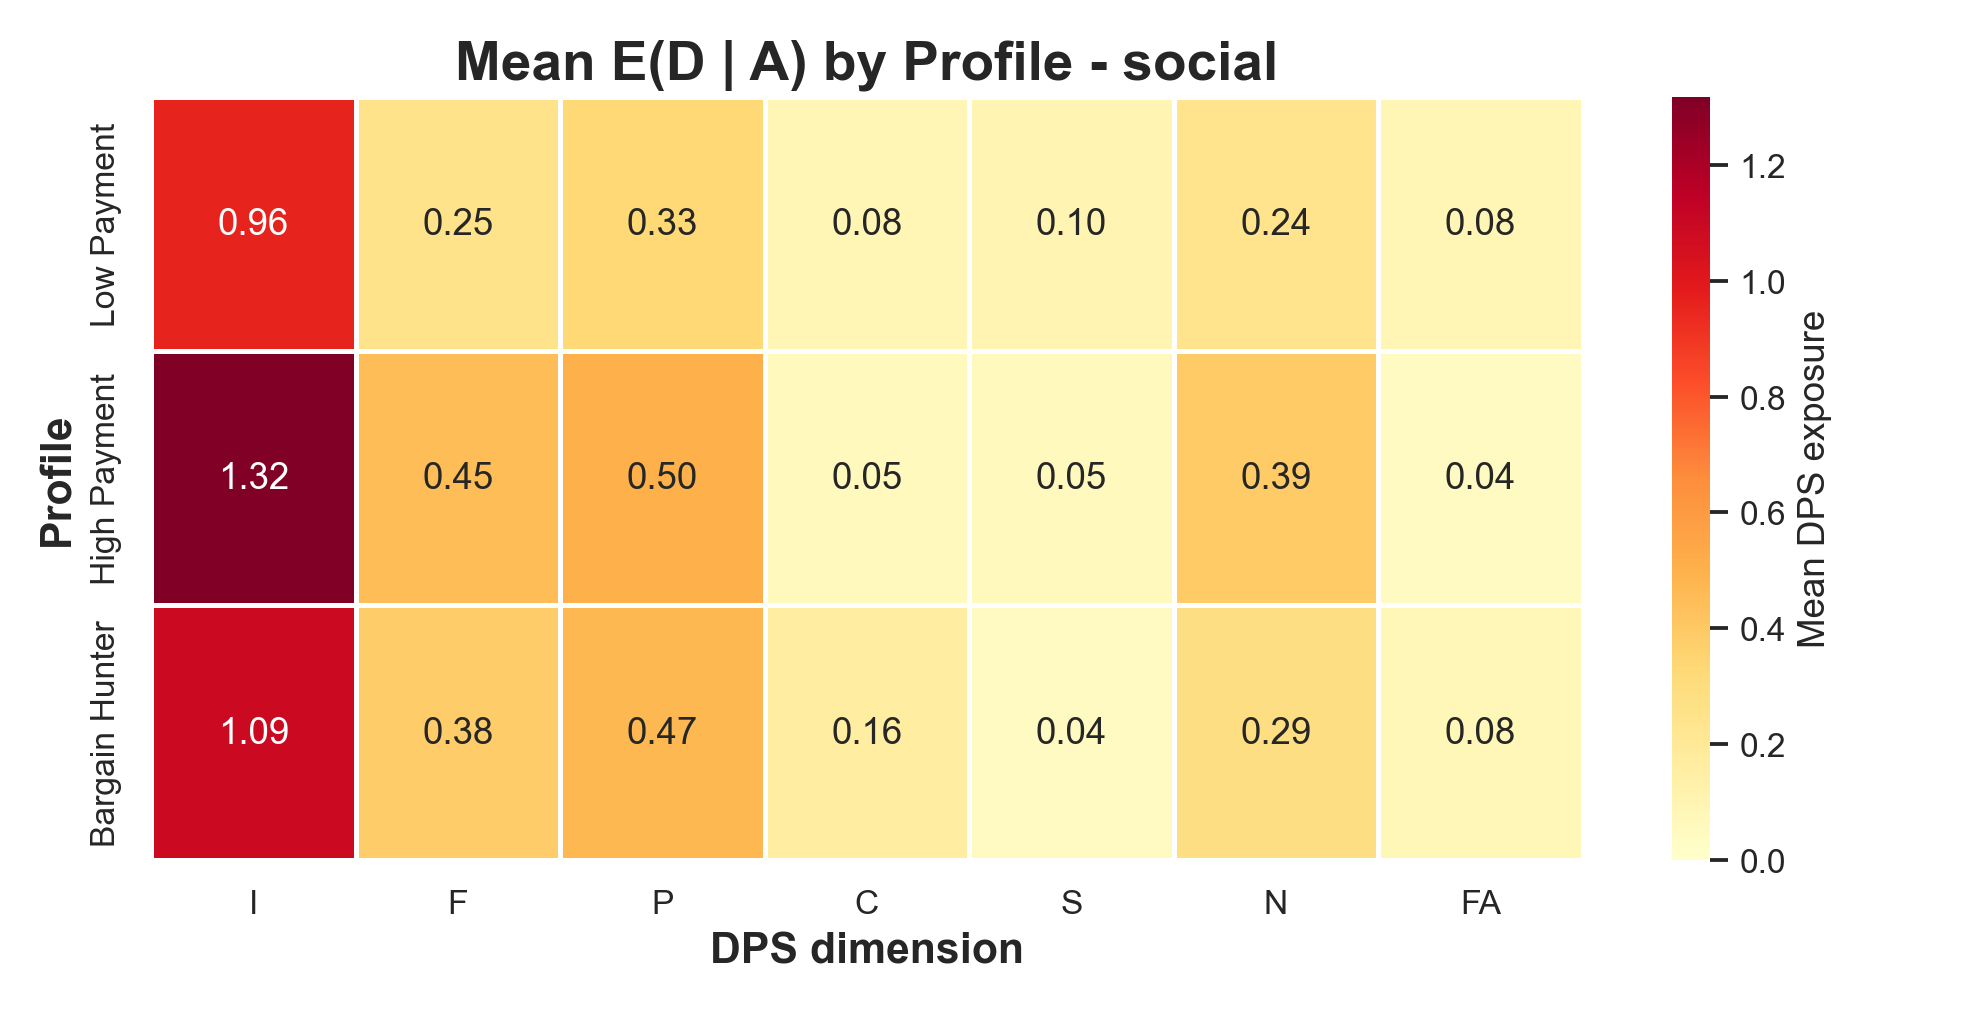
\includegraphics[width=0.95\linewidth]{figures/statistics/heatmap_mean_exposure_social.png}
    \caption{Mean DPS exposure heatmap for social applications.}
    \label{fig:category-heatmap-social}
\end{figure}

For e-commerce applications, the most prominent dimensions are Pressure, Sneaking, and Interface Interference. This pattern is consistent with the commercial structure of shopping interfaces. Users are frequently guided through product recommendation pages, discount panels, membership prompts, shopping carts, and checkout-related screens. In these contexts, applications may emphasize limited-time discounts, visually prioritize promotional options, preselect certain benefits, or make alternative choices less visible. The high-payment and bargain-hunter profiles are especially likely to encounter such interfaces because their keyword and action distributions lead them toward commercial decision points. These observations align with prior studies showing that shopping environments are common sites for scarcity messages, social proof, hidden costs, and other manipulative design strategies \cite{mathur2019darkpatterns}.

Food-delivery applications show consistently high Forced Action exposure in the project results. This may be associated with interface flows that require location access, login, phone verification, address selection, or permission granting before users can fully browse menus, place orders, or access coupons. Pressure and Nagging also appear in this category, often through repeated prompts for membership, coupons, delivery discounts, push notifications, or limited-time offers. Because food-delivery apps often combine urgent consumption contexts with location-based services and promotional systems, users may encounter multiple forms of commitment-requesting interfaces. However, this should be understood as an observed pattern in the audited sample rather than a universal property of all food-delivery applications.

Content platforms show a different exposure profile. Instead of checkout-oriented pressure, they more frequently involve login prompts, notification prompts, recommendation loops, and nagging. A user may be repeatedly encouraged to sign in, enable notifications, follow accounts, remain in the feed, or continue consuming recommended content. These mechanisms may not always correspond to direct commercial payment, but they can still shape user autonomy and attention. For example, recommendation loops may keep users in a sequence of suggested content, while notification prompts may repeatedly interrupt browsing. Such patterns suggest that dark pattern exposure in content platforms is often related to engagement retention rather than immediate purchase conversion.

Lifestyle service applications show more mixed patterns, including Contextual Deception, Friction, and promotional Pressure. These applications may include booking flows, service reservations, membership benefits, location-based recommendations, and promotional bundles. Contextual deception may appear when an interface leads users to expect one action but produces a different practical outcome, such as entering a promotional flow instead of completing a simple search or service selection. Friction may appear when cancellation, refusal, or dismissal requires more steps than acceptance. Promotional pressure may appear when service discounts, memberships, or limited-time benefits are emphasized during the decision process.

Taken together, the category-level results show that profile-dependent exposure interacts with app-domain characteristics. Commercially intensive categories tend to expose users to more decision-stage pressure, while engagement-oriented platforms tend to rely more on nagging and retention prompts. Service-oriented apps may combine promotional pressure with friction and contextual ambiguity. These findings reinforce the need to analyze dark patterns not only as isolated interface elements, but also as exposure patterns shaped by profile, behavior, app category, and interaction trajectory.

\chapter{Discussion}

\section{Why Exposure Differs Across Profiles}

The results of this project suggest that dark pattern exposure in mobile applications is shaped by the interaction trajectory through which an interface is reached. A dark pattern may exist somewhere inside an application, but it becomes measurable exposure only when a profile enters the relevant interface state and receives a positive DPS label. This distinction matters because the controlled profiles in this project differ in both interest distributions and behavior distributions. They therefore generate different action sequences, and those action sequences lead to different estimates of \(E(D \mid A)\).

The high-payment shopping profile is more likely to enter decision-sensitive contexts. Its behavior distribution makes product search, product-detail inspection, cart entry, membership evaluation, and checkout-related actions more probable. These states are close to monetization and conversion, so they are also the states where Interface Interference, Pressure, Sneaking, Friction, and Forced Action may become visible. A checkout-adjacent screen may emphasize a purchase button, preselect an add-on, display a limited-time offer, or make refusal less salient. When such screens appear repeatedly in the trajectory, they raise the relevant components of \(E(D \mid A)\) and produce positive components in \(\Delta(A_i,A_j)\) against a lower-intent profile.

The bargain-hunter profile reaches a different but similarly sensitive set of contexts. Searches for coupons, group buying, discounts, limited offers, and promotional rewards move the trajectory toward interfaces where scarcity and urgency may be part of the service logic. In DPS terms, these contexts can activate Pressure and Interface Interference labels through countdowns, inventory warnings, visually dominant promotional buttons, reward thresholds, or messages that frame delay as loss. The observed results, however, show that Pressure is category-dependent rather than uniformly strongest for the bargain-hunter profile. The profile does not need to be treated as a demographic group for this mechanism to matter. It is enough that its keyword and action distributions increase the probability of entering promotion-heavy interface states.

By contrast, the low-payment browsing profile more often remains in feed, search, and general browsing states. These states can still contain dark patterns, especially Forced Action, Nagging, notification prompts, or login gates. However, they are less consistently tied to purchase conversion, coupon redemption, or payment decisions. The difference is therefore not a simple high-risk versus no-risk contrast. It is a difference in the distribution of observed DPS vectors across trajectory states.

This interpretation keeps the causal claim narrow. The audit observes profile-conditioned exposure, not the internal policy that produced each screen. Higher Interface Interference for a profile, or category-specific differences in Pressure, can arise from profile-driven navigation, content-conditioned recommendation, platform personalization, or their interaction. The empirical contribution is to show that the resulting exposure distributions differ in measurable ways, using \(E(D \mid A)\), \(\Delta(A_i,A_j)\), running mean stabilization, and permutation-based validation as evidence.

\section{Dark Pattern Exposure as a Distributional Problem}

A central implication of this project is that dark pattern exposure should be studied as a distributional problem rather than a static presence problem. Much existing work asks whether an application or website contains dark patterns, how those patterns can be categorized, and how frequently they appear in collected interface samples \cite{gray2018darkpatterns,mathur2019darkpatterns,mathur2021whatmakesdark}. That work is necessary for defining the phenomenon. However, the presence of a manipulative interface element somewhere in an application does not determine which users encounter it, how often they encounter it, or at what decision point it appears.

The DPS framework makes this distinction operational. Each screenshot is one observed interface state, represented as \(D_t=[I_t,F_t,P_t,C_t,S_t,N_t,FA_t]\). A profile-level estimate \(E(D \mid A)\) is not a claim that the app has a fixed amount of manipulation; it is the empirical mean of DPS observations produced by a profile-conditioned trajectory. Depending on the analysis, \(D_t\) can be the raw numeric score vector or the binarized occurrence vector \(1[D_t>0]\). The running mean curves further show why a single screenshot is not enough. Early observations can be dominated by onboarding, a login wall, or one promotional popup, while later estimates become more stable as the trajectory accumulates additional interface states.

This framing changes the research question. Instead of asking only whether a dark pattern exists, the audit asks how DPS labels are distributed across profiles, apps, categories, and steps. A forced login screen may appear only after a coupon action. A countdown may appear only in a discount-search path. A preselected membership benefit may appear only near checkout. A cancellation obstacle may appear only after a subscription path has already been entered. These are exposure conditions, not merely interface inventory items.

The distributional view also explains why \(\Delta(A_i,A_j)\), \(L_1\) distance, and permutation tests are useful. Pairwise differences identify which DPS dimensions separate two profiles. The \(L_1\) distance summarizes the magnitude of the vector-level gap. Permutation tests ask whether the observed gap is larger than would be expected after random profile-label reassignment. Together, these measures shift dark pattern auditing from static detection toward profile-conditioned exposure analysis, while still keeping the evidence tied to observable interface states.

\begin{figure}[htbp]
    \centering
    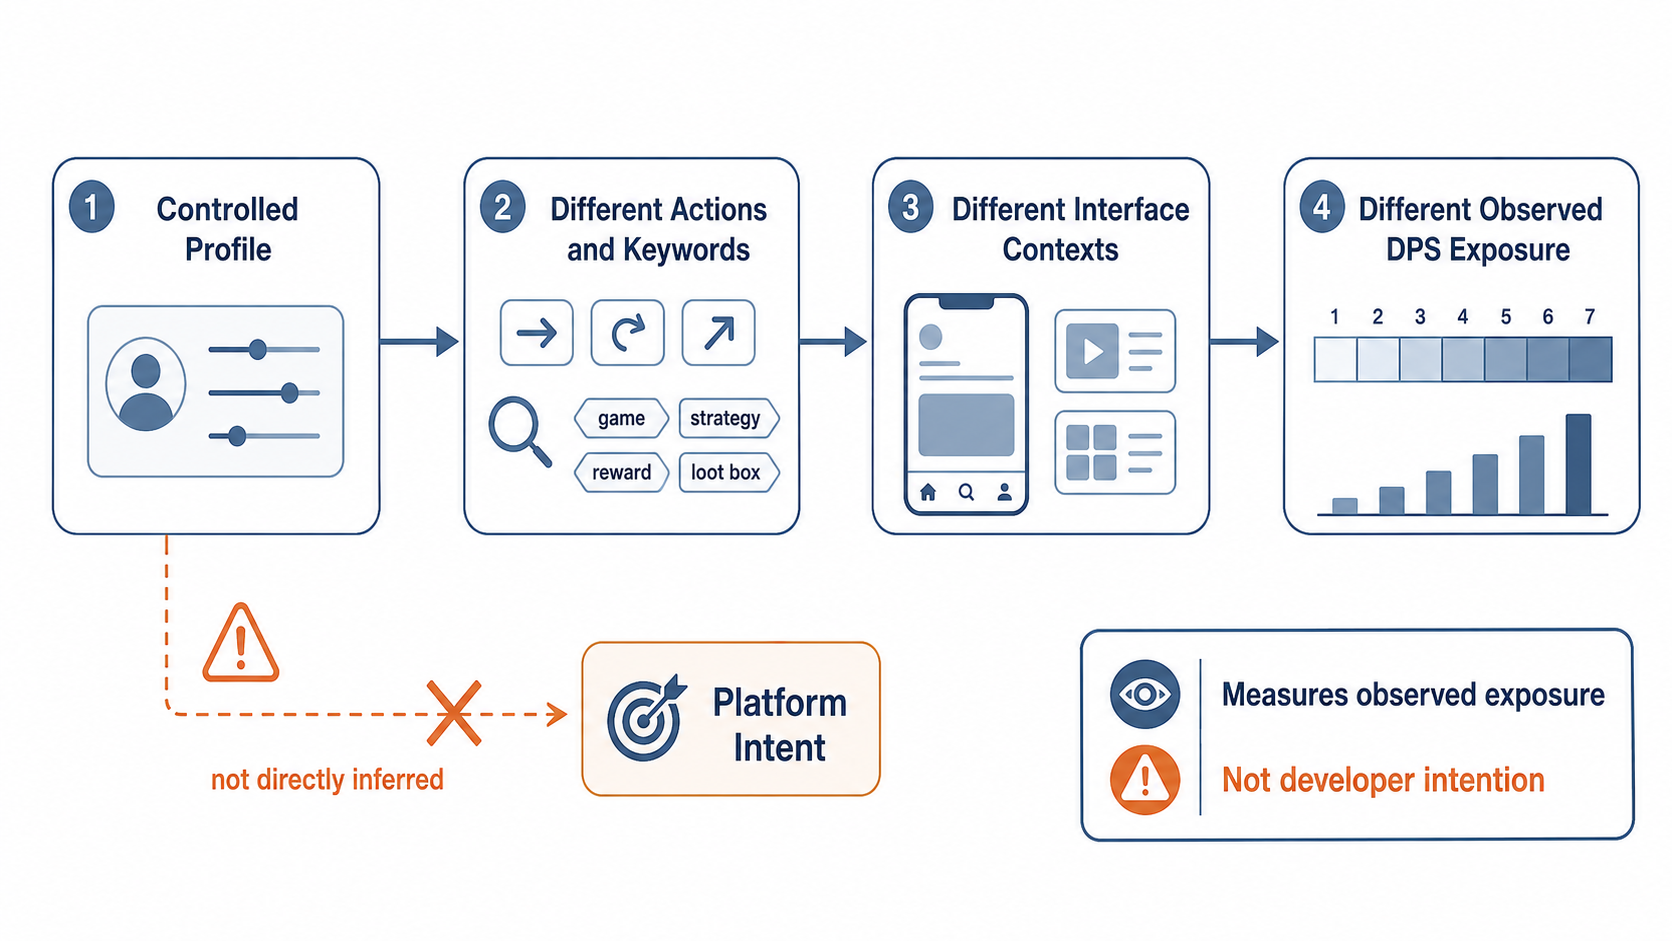
\includegraphics[width=0.95\linewidth]{figures/pictures/why_exposure_differs_across_profiles.png}
    \caption{Why Exposure Differs Across Profiles}
    \label{fig:why_exposure_differs_across_profiles}
\end{figure}

\section{Implications for Platform Accountability}

The distributional nature of dark pattern exposure has implications for platform accountability, but the implication is primarily methodological. Platforms should be evaluated not only by whether a dark pattern can be found, but by how DPS exposure is distributed across profile-conditioned trajectories. The relevant audit object is the exposure distribution \(E(D \mid A)\), together with profile gaps such as \(\Delta(A_i,A_j)\), rather than a single screenshot or a single default journey.

This framing avoids treating every profile difference as a moral accusation. Some differences are functionally expected. A profile that enters checkout more often will see more payment, membership, and delivery-choice interfaces. A profile that searches for coupons will see more promotion modules. The accountability question is whether these decision-sensitive contexts concentrate DPS mechanisms such as Pressure, Interface Interference, Sneaking, Friction, or Forced Action in ways that can be observed, measured, and compared across profiles.

A practical platform audit could therefore report profile-conditioned exposure distributions. Auditors could run the same application under high-payment, low-payment, bargain-seeking, and other controlled behavioral profiles; compute \(E(D \mid A, app)\) and \(E(D \mid A, category)\); compare profiles through \(\Delta(A_i,A_j)\) and \(L_1\) distance; and validate prominent gaps with permutation tests and corrected \(q\)-values. Such reporting would make clear whether a platform's pressure or interference exposure is broadly distributed, concentrated in purchase paths, concentrated in discount paths, or tied to access-control moments such as login and permissions.

The same logic can inform compliance and review processes. Sensitive flows such as subscription, payment, cancellation, coupon redemption, notification permission, and location permission should be audited as trajectories, not only as isolated screens. A platform-facing dashboard could track the running mean of each DPS dimension for major profile classes and flag cases where exposure remains elevated after repeated interaction steps. The goal of such tools is not to infer hidden intent from outside the system. It is to make profile-conditioned exposure measurable enough for review, comparison, and redesign.

\section{Implications for Users}

From the user perspective, the findings suggest that personal experience with an application may be an incomplete view of the platform's interface environment. A user sees the screens generated by their own trajectory, not the full distribution of screens that other profiles may encounter. If one user rarely enters checkout, they may underestimate payment-stage Pressure or Sneaking. If another user frequently searches for coupons, they may overestimate how central countdowns and scarcity messages are to the application as a whole.

High-payment users may face stronger commercial interface exposure because their behavior brings them closer to decision points. They may encounter membership prompts, limited-time offers, add-on recommendations, or interface designs that make payment-related actions visually salient while making refusal less convenient. In DPS terms, the relevant risk is not a single promotional screen, but repeated positive observations in dimensions such as Interface Interference, Pressure, Sneaking, or Friction across the trajectory.

Bargain hunters may face a different but related exposure pattern. Searches for discounts, coupons, flash sales, and promotional opportunities can increase contact with scarcity cues, countdown timers, social proof, and reward thresholds. These mechanisms can frame delay as loss or make benefits appear conditional on immediate participation. Because bargain-seeking behavior is often motivated by cost sensitivity, the category-specific distribution of pressure-heavy screens along this path deserves attention even when the same app also contains ordinary browsing interfaces.

Low-payment browsing users should not be treated as unaffected. They may avoid many checkout-specific screens, but still encounter Forced Action, repeated notification prompts, login gates, nagging pop-ups, permission requests, or friction when dismissing recommendations. Their \(E(D \mid A)\) may therefore be lower in some commercial dimensions while remaining meaningful in access-control or engagement-retention dimensions.

The broader lesson is that individual reports about an application's interface can be biased by trajectory. A user can accurately describe what they saw and still miss exposure patterns concentrated in other profile-conditioned paths. For this reason, user protection should not rely only on individual awareness or anecdotal comparison. It requires audits that sample multiple trajectories and estimate how DPS exposure is distributed across them.

\section{Implications for Researchers}

For researchers, this project suggests a bridge between dark pattern taxonomy and algorithm auditing. Dark pattern research provides the DPS vocabulary for identifying manipulative interface mechanisms, while audit methodology provides controlled procedures for comparing black-box outputs across profiles. The unit of analysis is therefore not only the screenshot, but the trajectory log that explains how the screenshot was reached.

Future work should strengthen three parts of this design. First, trajectory logging should record not only screenshots and DPS labels, but also actions, keywords, app states, timestamps, pop-up recurrence, dismissal attempts, and transitions into payment, subscription, coupon, permission, or cancellation flows. This would make it easier to distinguish decision-sensitive contexts from general browsing contexts and to interpret changes in the running mean over time.

Second, multi-profile auditing should be expanded beyond the three profiles used here while preserving experimental control. Additional profiles could vary purchase intent, coupon sensitivity, subscription history, permission refusal behavior, account age, or task goal. The purpose would not be to map demographic identity directly onto exposure, but to test how behaviorally defined profiles change \(E(D \mid A)\), \(E(D \mid A, app)\), and \(E(D \mid A, category)\).

Third, statistical validation should remain central. Pairwise differences \(\Delta(A_i,A_j)\) identify which DPS dimensions differ, but those differences should be evaluated with running mean stabilization, permutation tests, corrected \(q\)-values, \(L_1\) distance, and association measures such as Cramér's \(V\). This combination helps separate stable profile-conditioned patterns from isolated interface events or small-sample fluctuation.

More broadly, the project indicates that personalization and path dependence should become central concerns in dark pattern research. Static inspection can show that a manipulative design exists, but it cannot show how exposure is allocated across users and situations. By treating dark pattern exposure as profile-conditioned, measurable, and statistically testable, future research can study deceptive interfaces as dynamic components of personalized digital environments while keeping claims tied to observable evidence.

\chapter{Limitations}

This project provides a profile-aware framework for auditing differential dark-pattern exposure in mobile applications. By combining controlled profile construction, repeated interaction trajectories, DPS annotation, and profile-conditioned exposure estimation, the framework makes it possible to compare how different user profiles are associated with different patterns of deceptive interface exposure. The limits discussed below do not weaken that contribution. They define the scope in which the report makes a defensible claim: it measures observed profile-conditioned exposure, not platform-internal algorithms, developer intent, or a full reconstruction of hidden personalization logic.

\section{Manual Annotation}

The limitation is that DPS labels are assigned manually. Each interaction record is annotated against the seven-dimensional DPS vector, so the final exposure estimates depend on human interpretation of interface context, wording, salience, and action affordances. This matters because some cases are intrinsically borderline: a promotional countdown can be ordinary marketing in one setting and pressure in another, and a misleading-looking interface can be difficult to separate from low-quality design.

This report mitigates the risk by using a fixed taxonomy, written annotation rules, and a profile-controlled audit setting. Those constraints do not remove judgment, but they make the judgment comparable across apps and profiles. In other words, the study is not trying to mechanically detect every deceptive element; it is building a consistent measurement procedure for observed exposure. That is sufficient for the current research goal because the main comparison is between controlled profiles under the same annotation protocol.

Future work should add multiple annotators, measure inter-annotator agreement, and use adjudication to refine ambiguous cases. Automated or semi-automated detectors can then be introduced as a scaling layer, but they should remain tied to the same DPS definitions rather than replacing them. The present report remains effective because it establishes a transparent baseline that makes later automation auditable and comparable.

\section{Fixed Interaction Budget}

The limitation is that every app-profile pair is observed under a fixed 30-step interaction budget. This matters because some exposure mechanisms are cumulative: recommendations, promotions, retention prompts, and permission requests may only appear after longer account histories or repeated engagement.

This report mitigates that limitation by treating 30 steps as a controlled audit window rather than a claim about full-life app usage. The running mean curves show that several exposure estimates stabilize within the available budget, so the fixed-length design still provides a meaningful basis for cross-profile comparison. The key value of the study is comparative measurement under identical conditions, not exhaustive simulation of user lifetime behavior.

Future work should vary trajectory length, use convergence-based stopping rules, or run repeated audits over longer periods. That extension belongs in Chapter 12, but it does not reduce the usefulness of the present results: within the chosen window, the framework can still distinguish profile-conditioned exposure patterns in a reproducible way.

\section{Static Profiles}

The limitation is that profiles are static once the audit starts. Each profile is defined by a fixed keyword distribution and a fixed action distribution, so the framework does not model how interests or behaviors evolve during the session.

This matters because real users are adaptive. Their later actions can differ from their initial intent, and platform responses may in turn alter what they see next. Static profiles therefore simplify a dynamic social and technical process into a controlled initial condition. The limitation is methodological, not conceptual: it means the report studies exposure conditioned on a specified profile, not exposure under a fully evolving user model.

The report mitigates this by making the profile definition explicit and reproducible. Static profiles isolate the effect of controlled starting conditions, which is exactly what is needed to compare observed exposure across groups. That makes the current design effective for the report's objective: it identifies whether the same app presents different observable exposure patterns under different controlled profiles.

Future work should introduce dynamic profile updates so that profiles can respond to accumulated history. Chapter 12 already points to this extension. For the current report, the static design remains valuable because it removes one major source of confounding and keeps the exposure comparison interpretable.

\section{Limited App Scope}

The limitation is that the audit covers 16 mobile applications rather than the full mobile ecosystem. This matters because app categories, regions, business models, and release cycles differ, so no finite sample can justify universal claims about all mobile apps.

This report mitigates that limitation by sampling across multiple categories and by presenting category-level as well as app-level results. That design does not claim representativeness in a statistical-population sense; instead, it provides cross-app evidence that profile-conditioned exposure is observable in a diverse set of real applications. The project is therefore still effective because it demonstrates the phenomenon in more than one setting, rather than relying on a single app or a toy example.

Future work should broaden the sample, repeat audits across time, and record version changes more systematically. Those extensions are discussed in Chapter 12. The present scope is still meaningful because it establishes that the framework works across multiple common app types and can surface differences that are not reducible to one product category.

\section{No Strong Causal Claim}

The limitation is that the framework supports observational inference, not strong causal attribution. The report measures observed profile-conditioned exposure, denoted as $E(D \mid A)$, and compares exposure distributions across profiles. It does not identify the platform's internal ranking policy, personalization rule, or developer intent.

This matters because the same exposure gap can be produced by several mechanisms: profile-driven navigation, history-dependent recommendation, ordinary interface branching, or general design differences that are unrelated to targeted manipulation. A statistically significant difference therefore shows that the profiles do not experience the same observable interface environment, but it does not by itself explain why.

The report mitigates this by using careful language, by pairing exposure estimates with permutation-based validation, and by limiting the interpretation to what is actually observed. That restraint strengthens the paper rather than weakening it: the contribution is a defensible black-box audit of visible outcomes, which is exactly the right level of evidence for the available data.

Future work should use designs that separate direct effects from mediated effects, or otherwise support stronger counterfactual claims. Chapter 12 already outlines that direction. For the current report, the observational framing is still effective because it avoids overclaiming while still showing that profile-conditioned exposure differences are measurable and repeatable.

\section{Manual Persona Design}

The limitation is that personas are designed manually. Keyword pools and action probabilities are chosen by the researchers rather than learned from a large corpus of real user traces.

This matters because manual construction can omit mixed motives, context switching, and population heterogeneity. It may also embed the researcher's assumptions about what counts as a high-payment shopper, a low-payment browser, or a bargain hunter. At the same time, the design is intentional: the study is built to compare controlled experimental profiles, not to infer or reproduce the identities of real users.

The report mitigates this by keeping profiles narrow, explicit, and non-demographic. That choice is part of the method's strength, not merely a compromise. It makes the audit reproducible, reduces privacy risk, and keeps the measurement focused on behavior-conditioned exposure rather than sensitive user classification. In that sense, the project remains effective because the personas function as controlled probes, which is the proper role of personas in this report.

Future work should estimate profile parameters from privacy-preserving behavioral data or use synthetic agents to generate richer persona dynamics. Chapter 12 covers that extension. The current manual design still serves the study well because it provides a transparent baseline for observing how the same apps respond to clearly specified interaction styles.

\chapter{Future Work}

This project provides an initial profile-aware auditing framework for measuring differential dark pattern exposure in mobile applications. However, as discussed in the limitations, the current framework remains partly manual, uses static profiles, and evaluates a bounded set of applications and interaction steps. Future work can extend the framework in several directions so that profile-conditioned dark pattern exposure can be measured more automatically, more realistically, and at a larger scale.

\section{Automatic DPS Detection}

A major direction for future work is the automatic detection of DPS dimensions from mobile interface screenshots and interaction traces. In the current project, DPS annotation relies on human judgment, which is useful for interpretability but costly to scale. Manual annotation also introduces potential inconsistency, especially when a screenshot contains ambiguous interface elements or multiple dark pattern mechanisms at the same time. Future versions of the framework could therefore combine optical character recognition, computer vision, UI element detection, and multimodal large language models to identify dark pattern evidence automatically.

For example, OCR could extract textual cues such as countdown messages, urgency phrases, discount claims, membership reminders, or refusal-related wording. Computer vision models could identify layout-level features such as button size asymmetry, color salience, hidden close buttons, pop-up overlays, and obstructed exit paths. UI element detection could further help distinguish between accept buttons, reject buttons, checkout links, recommendation cards, and subscription prompts. These signals could then be mapped into the seven DPS dimensions: Interface Interference, Friction, Pressure, Contextual Deception, Sneaking, Nagging, and Forced Action. Recent work on dark pattern taxonomy and detection suggests that automated classifiers may help reduce the burden of manual inspection, although full automation should still be treated carefully because dark pattern interpretation often depends on context \cite{li2024comprehensive,mathur2019darkpatterns}.

A practical future system could use a hybrid pipeline. First, screenshots and UI trees would be processed by OCR and visual detectors. Second, a dark pattern classifier or multimodal model would produce candidate DPS labels with confidence scores. Third, human annotators would only review uncertain or high-risk cases. This would reduce annotation cost while preserving quality control. Such an approach would make it possible to audit many more applications and interaction records than the current 1,440-record experiment.

\section{LLM Agent-based App Exploration}

Another important extension is to replace simple probabilistic action generation with LLM agent-based mobile app exploration. In the current framework, user behavior is modeled as a profile-conditioned probability distribution over actions. This design is controlled and reproducible, but it simplifies how real users interact with mobile applications. Real users do not merely sample actions from fixed probabilities; they read interface content, react to recommendations, compare options, abandon tasks, and enter decision-related flows based on evolving goals.

Future work could use LLM agents to explore apps in a more natural and goal-directed manner. Each agent could be assigned a profile-specific objective, such as searching for high-value electronics, browsing casually without purchase intent, or finding coupons and limited-time discounts. The agent could observe the current screen, interpret interface content, decide the next action, and record why that action was chosen. This would allow the audit to capture more realistic trajectories than fixed action templates alone.

LLM agents could also enter decision-related flows more intelligently. For instance, a high-payment shopping agent might compare recommended items and proceed toward checkout when the interface appears relevant, while a bargain-hunter agent might actively search for discount codes, flash sales, or membership rewards. This would make the framework closer to real profile-conditioned behavior while still preserving audit control. Similar to sock-puppet and agent-based audits in recommendation systems, the key challenge would be balancing realism with reproducibility \cite{srba2023youtube,haroon2023youtubeaudit}. Future work should therefore log agent prompts, observations, actions, and decision rationales so that the exploration process remains inspectable.

\section{Dynamic User Modeling}

The current framework uses static user profiles. Each profile has a predefined interest distribution and behavior distribution, and these settings remain unchanged during the 30-step interaction process. This is useful for a first controlled experiment, but it does not fully represent real users. In actual mobile applications, user profiles may evolve as users search, click, browse, ignore recommendations, open payment pages, or repeatedly respond to pop-ups.

Future work could model user profiles dynamically. Instead of treating profile \(A_t\) as fixed, the framework could update the profile after each interaction according to the user’s history:

\[
A_{t+1} = f(A_t, history_t)
\]

In this formulation, \(A_t\) denotes the user profile at step \(t\), while \(history_t\) represents the accumulated interaction history up to that point. The function \(f\) updates the user representation based on observed actions, searched keywords, clicked items, dwell time, and decision-related visits. This would better reflect real users whose interests and behaviors are not static but change through interaction.

Dynamic user modeling would also allow the audit to examine whether dark pattern exposure increases, decreases, or changes type as a profile becomes more established. For example, a bargain-hunter profile might initially receive general shopping recommendations but gradually encounter more discount-related pressure or membership prompts. A high-payment profile might be routed more often into checkout-adjacent flows after repeated high-value searches. These possibilities should not be interpreted as causal claims without stronger evidence, but dynamic modeling would make such temporal patterns observable and testable. Prior work on user profiling and sequential recommendation provides useful conceptual support for this direction \cite{purificato2024usermodeling,lian2021multiinterest,hou2022unisrec}.

\section{Larger-scale Auditing}

The current experiment covers 16 applications, 3 profiles, and 30 steps per profile-app pair, producing 1,440 interaction records and 10,080 DPS labels. This scale is sufficient for a course project and demonstrates the feasibility of profile-conditioned exposure estimation. However, larger-scale auditing is necessary before making broader claims about mobile app ecosystems.

Future work could expand the framework across more applications, more categories, more geographic regions, more app versions, and longer observation windows. Different app categories may exhibit different dark pattern mechanisms. For example, food-delivery apps may show consistently high forced-action exposure, while shopping apps may show stronger pressure or interface interference around promotional and checkout flows. A larger audit could test whether these category-level patterns remain stable across platforms and regions.

Repeated audits over time would also be valuable. Mobile applications frequently update their interfaces, recommendation strategies, promotion mechanisms, and consent flows. A single audit captures only one time window. By repeating the same profile-conditioned audit monthly or across major app versions, researchers could observe whether dark pattern exposure is persistent, seasonal, or associated with specific platform updates. This would improve the generalizability and temporal validity of the framework.

\begin{figure}[htbp]
    \centering
    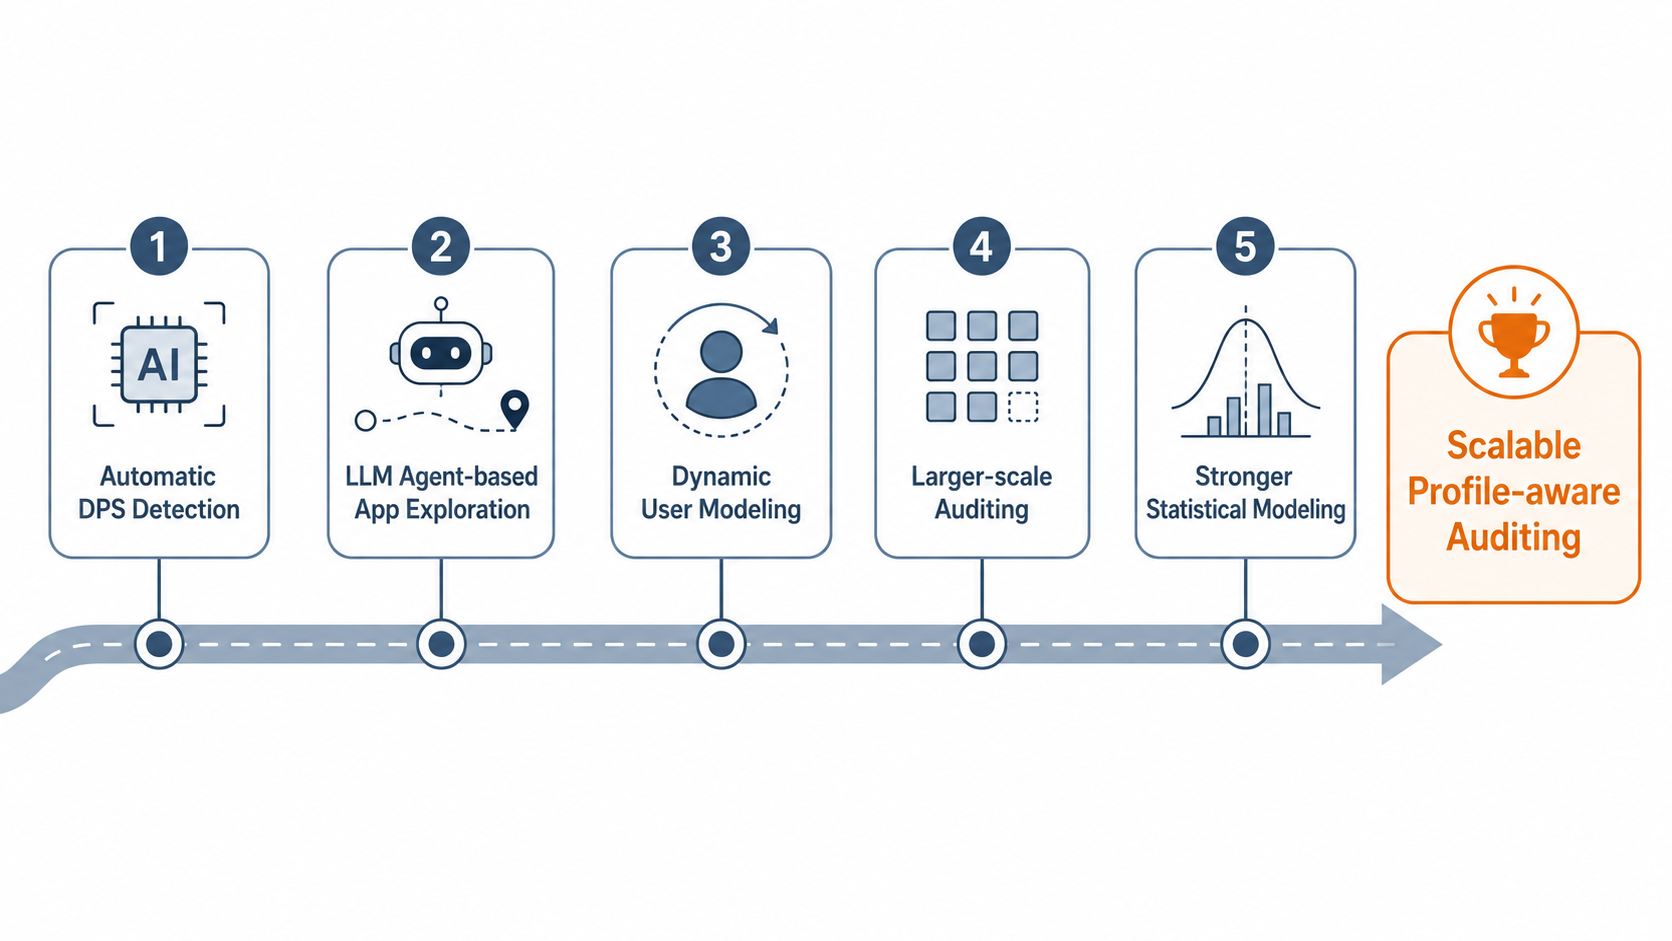
\includegraphics[width=0.95\linewidth]{figures/pictures/future_work_roadmap.png}
    \caption{Future Work Roadmap}
    \label{fig:future_work_roadmap}
\end{figure}

\section{Stronger Statistical Modeling}

Finally, future work can strengthen the statistical analysis of profile-dependent exposure. The current framework already uses profile-conditioned exposure estimation \(E(D \mid A)\), pairwise exposure differences \(\Delta(A_i, A_j)\), permutation tests, q-values, L1 distance, and Cramér’s V. These methods provide useful evidence of association between user profile and DPS exposure, but more advanced models could provide a clearer decomposition of where the differences come from.

Mixed-effects models could account for the fact that observations are nested within apps, app categories, profiles, and interaction steps. Bootstrap confidence intervals could quantify uncertainty around exposure estimates without relying too heavily on parametric assumptions. Longitudinal analysis could examine whether exposure converges, accumulates, or changes across interaction trajectories. These methods would make the framework more statistically robust, especially when extended to larger datasets.

A particularly important direction is causal mediation analysis or profile-action-DPS decomposition. In the current setting, a profile may receive different exposure partly because the platform personalizes the interface directly, but also partly because different profiles take different actions. For example, the high-payment profile may encounter more pressure-related exposure because it enters checkout pages more often, not necessarily because the platform directly targets that profile with pressure. Mediation analysis could help separate these possibilities by estimating how much of the profile difference is associated with action pathways such as search behavior, recommendation clicks, or decision-interface visits. Such analysis would not automatically prove causality, but it would provide a more careful way to distinguish direct profile-associated exposure from exposure mediated by interaction behavior.

Together, these future directions would extend the current framework from a controlled course-scale audit into a more automated, adaptive, and statistically rigorous system for studying personalized dark pattern exposure in mobile applications.

\chapter{Ethical Considerations}

Ethical considerations are central to this project because the proposed framework studies user-facing interface exposure under controlled profile conditions. Although the project does not intervene in application back-end systems or attempt to infer real users' private characteristics, it still involves systematic interaction with mobile applications, screenshot collection, and human annotation of potentially manipulative interface mechanisms. Therefore, the framework should be understood as a measurement and accountability approach rather than a tool for exploitation. This section discusses four ethical aspects of the study: the exclusion of sensitive demographic attributes, data privacy protection, responsible auditing boundaries, and ethical practices in human annotation.

\section{Avoiding Sensitive Attributes}

A key ethical design choice in this project is that controlled profiles are constructed using interests and behaviors rather than sensitive demographic attributes. In other words, the high-payment shopping profile, low-payment browsing profile, and bargain-hunter profile are defined by keyword distributions and interaction-action distributions, not by age, gender, income, ethnicity, religion, disability, or other personal characteristics. This decision is important because demographic attributes often carry heightened privacy risks and may introduce additional ethical concerns when used to simulate or compare user groups.

The exclusion of demographic attributes also reduces the risk that the audit could be interpreted as profiling real individuals or reproducing discriminatory categories. While prior user modeling research often discusses interests, behaviors, preferences, and attributes as possible components of user profiles, this project intentionally adopts a narrower and more controllable representation for auditing purposes \cite{eke2019userprofiling,purificato2024usermodeling}. Interests are operationalized as probability distributions over keywords, and behaviors are operationalized as probability distributions over interaction actions. This allows the study to examine whether different interaction styles are associated with different dark pattern exposure without making claims about protected or sensitive social groups.

This choice also improves reproducibility. Demographic attributes are difficult to verify, ethically sensitive to simulate, and often entangled with broader social and economic contexts. In contrast, keyword pools and action probabilities can be explicitly documented, reused, and modified by other researchers. Therefore, avoiding sensitive attributes does not weaken the audit design; rather, it makes the project more ethically constrained, methodologically transparent, and suitable for a course-scale measurement study.

\begin{figure}[htbp]
    \centering
    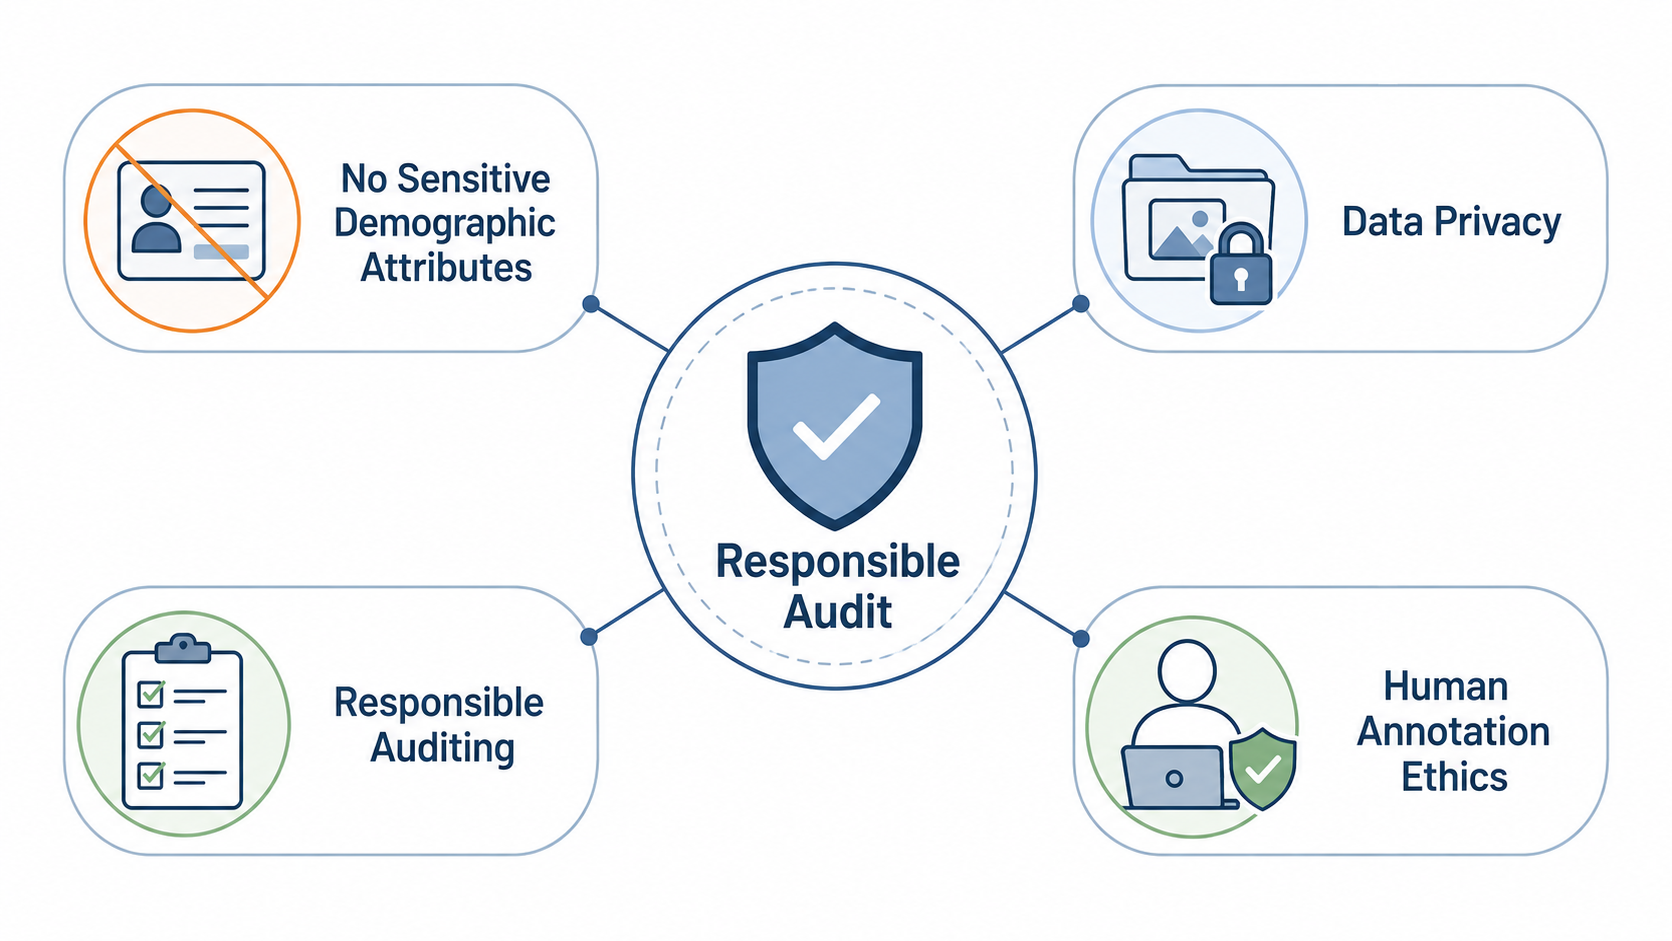
\includegraphics[width=0.95\linewidth]{figures/pictures/ethical_guardrails.png}
    \caption{Ethical Guardrails}
    \label{fig:ethical_guardrails}
\end{figure}

\section{Data Privacy}

The project relies on screenshots and interaction records, and these materials may contain sensitive information even when the accounts are newly created or controlled. For example, screenshots may accidentally capture account names, phone numbers, addresses, location information, payment interfaces, order details, recommendation histories, or other personal identifiers. Because the purpose of the study is to evaluate interface design features rather than personal information, such data should be blurred, removed, cropped, or excluded before analysis and presentation.

The dataset should retain only the information necessary for identifying and annotating dark pattern mechanisms. For instance, a screenshot showing a forced registration prompt, an obstructive cancellation path, or a pressure message may be useful for DPS annotation. However, the same screenshot should not preserve unrelated user identifiers or transaction details. This distinction is important because dark pattern auditing concerns the structure and behavior of the interface, not the private identity of the account holder.

Data minimization should therefore guide the entire workflow. Raw screenshots should be stored only when necessary, access should be limited to project members, and any public report figures should be carefully sanitized. If a report figure presents an example of interface interference or forced action, it should display only the relevant interface region. Similarly, annotation examples should describe interface mechanisms without including personal account information. These practices are consistent with the broader privacy principle that research data should be limited to what is necessary for the stated measurement objective.

\section{Responsible Auditing}

The goal of this project is not to attack, exploit, bypass, or disrupt mobile applications. The framework is designed to evaluate user-facing exposure to potentially manipulative interface practices under controlled profiles. This distinction is ethically important. The audit treats applications as black-box systems and records observable interface outcomes during ordinary interaction trajectories, following the general logic of external platform audits \cite{sandvig2014auditing,hannak2013personalization}. It does not attempt to access internal databases, reverse engineer private systems, overload services, circumvent authentication, or manipulate other users.

Responsible auditing also requires that the interaction procedure remain within normal user interaction boundaries. The profiles perform actions such as searching, browsing, scrolling, opening decision-related pages, closing pop-ups, or returning to previous screens. These actions resemble ordinary user behavior and are used only to observe whether dark pattern exposure differs across controlled profiles. The framework therefore measures what the application chooses to display in response to normal interactions, rather than forcing the application into abnormal states.

This ethical boundary also affects how findings should be interpreted. The project can report that certain profiles are associated with stronger exposure to interface interference or pressure-related mechanisms, or that some app categories show consistently high forced-action exposure. However, it should avoid overstating causality or claiming intentional discrimination without additional evidence. The appropriate interpretation is that the observed interface exposure patterns suggest profile-dependent differences that merit further investigation and accountability-oriented discussion.

\section{Human Annotation Ethics}

Human annotation is necessary because the DPS vector captures interface mechanisms that may require contextual judgment. However, annotation work should be designed to protect annotators as well as the privacy of the data subjects represented in screenshots. Annotators should not be exposed to unnecessary personal information. Before annotation, screenshots should be sanitized where possible, and annotation instructions should direct attention to visible interface mechanisms rather than user identity, account history, or personal content.

The annotation guidelines should define each DPS dimension in terms of observable evidence. For example, Interface Interference should be judged based on visual prominence, layout manipulation, or unequal presentation of options; Friction should be judged based on additional steps required to reject, cancel, or exit; Pressure should be judged based on countdowns, urgency messages, scarcity cues, or emotional persuasion; and Forced Action should be judged based on whether the interface requires an unrelated action before the user can proceed. This mechanism-focused approach helps reduce subjective moral judgment and keeps the annotation task aligned with prior dark pattern taxonomies \cite{gray2018darkpatterns,mathur2019darkpatterns,mathur2021whatmakesdark}.

Ambiguous cases should be discussed based on visible interface evidence rather than annotator assumptions. If a screenshot does not provide enough context to determine whether a design is deceptive, coercive, or merely inconvenient, the annotation should reflect that uncertainty through conservative labeling or discussion among annotators. This is especially important because dark pattern labels can carry normative implications. A responsible annotation process should therefore prioritize consistency, transparency, and evidence-based reasoning. In this sense, the DPS annotation framework is not only a technical measurement instrument, but also an ethical procedure for making claims about manipulative interface exposure in a careful and accountable manner.

\chapter{Conclusion}
\label{sec:conclusion}

This report has examined dark patterns not only as interface elements that may be present in an application, but also as exposure patterns that may vary across profile-conditioned interaction trajectories. This distinction matters because a user does not encounter an entire application at once. A user encounters a sequence of screens shaped by actions, searches, recommendations, prompts, and decision points. Profile-aware auditing therefore asks a more specific accountability question than static inspection: who encounters which forms of dark pattern exposure, how often, and under what behavioral conditions.

The proposed framework measures this problem through controlled profiles, repeated trajectories, and screenshot-level DPS annotation. Each profile is defined by interest and behavior distributions rather than demographic identity. Each observed screen is converted into a DPS vector covering Interface Interference, Friction, Pressure, Contextual Deception, Sneaking, Nagging, and Forced Action. Aggregating these vectors gives profile-conditioned exposure \(E(D \mid A)\), while pairwise comparisons provide differential exposure between profiles. In this design, dark pattern exposure is treated as a measurable distribution over interaction states, not as a single binary property of an app.

The empirical audit applied the framework to 16 apps, 3 profiles, and 30 steps for each app-profile pair, yielding 1,440 records and 10,080 DPS labels. The results suggest that exposure is unevenly distributed across controlled profiles. High-payment shopping and bargain-hunter trajectories more often encounter Pressure and Interface Interference, consistent with their movement toward checkout, membership, coupon, and promotion-heavy states. Low-payment browsing generally shows lower commercial-pressure exposure but still encounters Forced Action, Nagging, and access-control prompts. Category-level results further suggest that commercial, service, and engagement-oriented apps concentrate different DPS dimensions in different parts of the interaction path.

\begin{figure}[htbp]
    \centering
    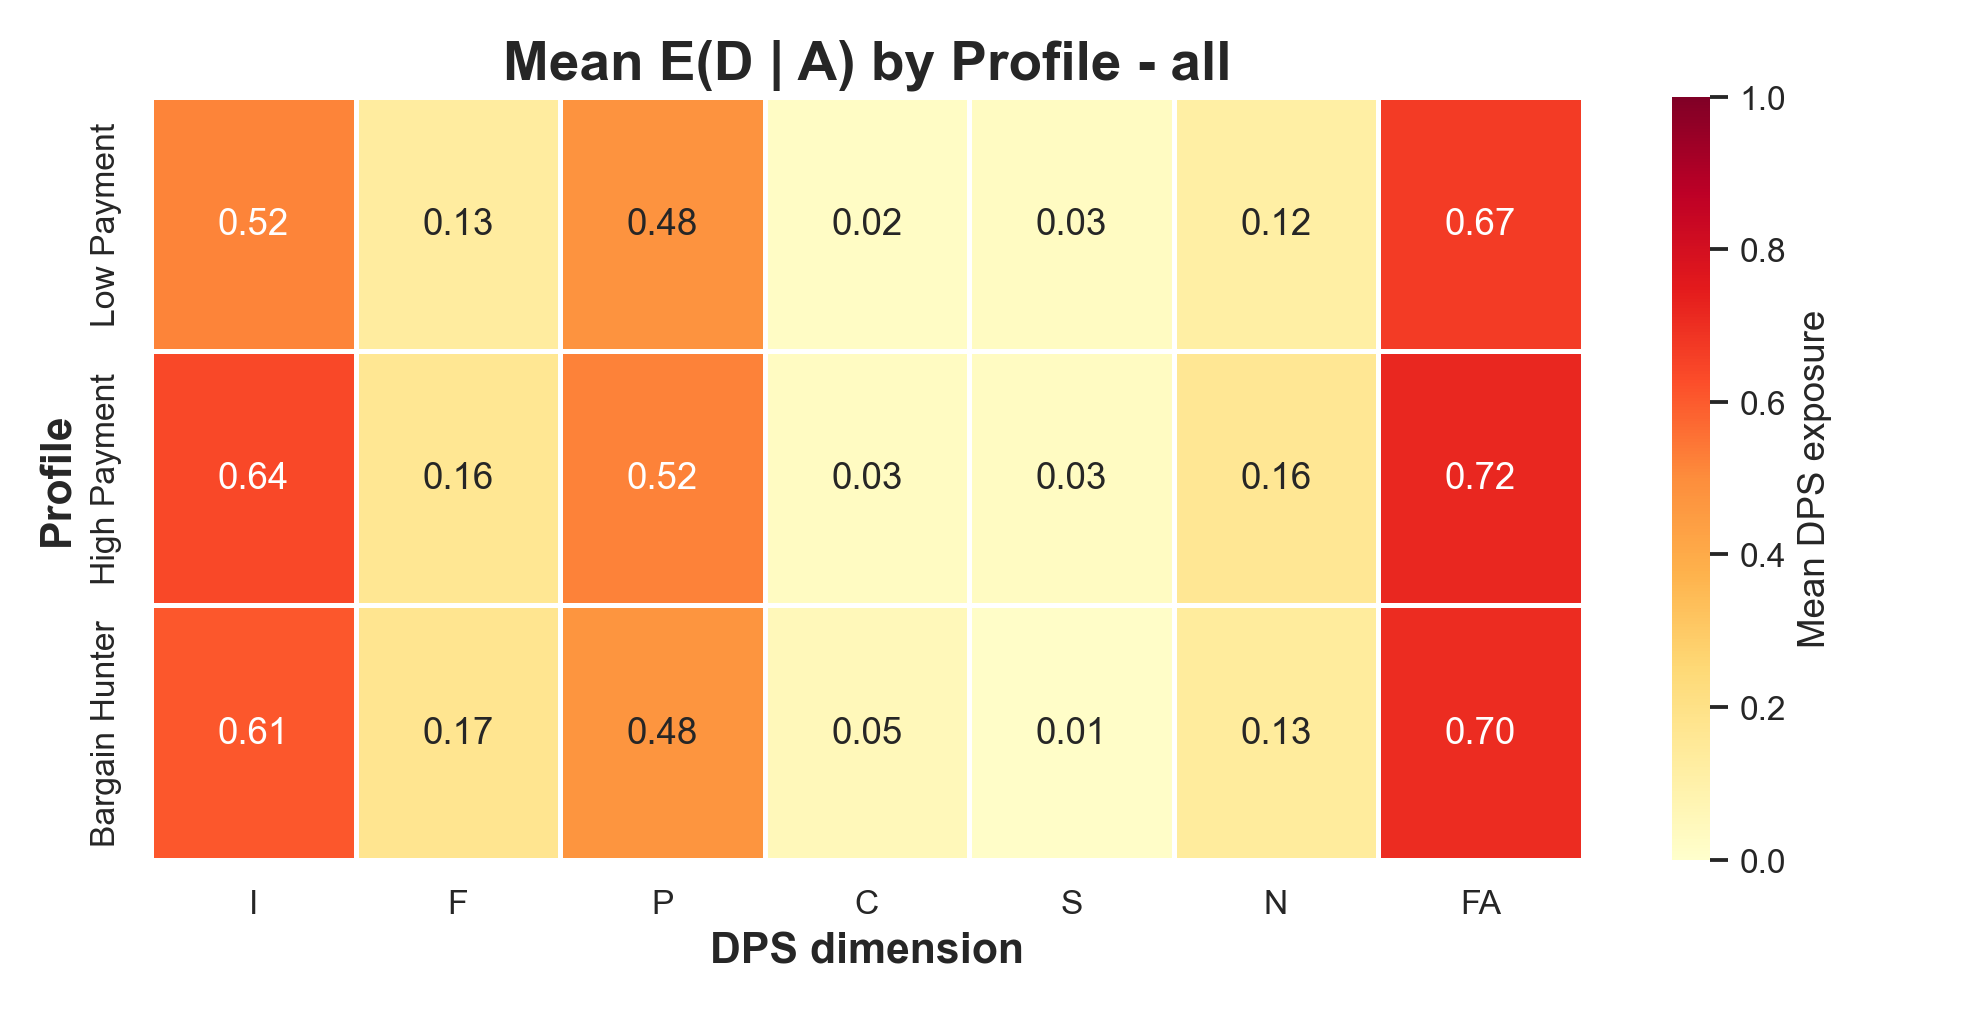
\includegraphics[width=0.95\linewidth]{figures/statistics/heatmap_mean_exposure_all.png}
    \caption{Summary heatmap of mean DPS exposure across all audited applications and controlled profiles.}
    \label{fig:conclusion-summary-heatmap}
\end{figure}

These findings do not imply deliberate profile-based manipulation. The audit observes visible outputs under controlled conditions; it does not inspect internal ranking, personalization, promotion, or interface-generation mechanisms. Differential exposure may arise from personalization, from rule-based app flows, from ordinary navigation differences, or from the fact that different profiles enter different decision contexts. The appropriate claim is therefore observational: in this dataset, profile-conditioned trajectories are associated with different DPS distributions.

Future work should extend the framework in several directions. Automatic or semi-automatic DPS annotation could reduce manual labeling cost while preserving human review for ambiguous cases. LLM-agent exploration could generate more realistic goal-directed trajectories than fixed probabilistic action sampling. Dynamic user modeling could examine how exposure changes as profiles accumulate interaction history. Larger audits across more apps, regions, versions, and time windows would improve external validity, while stronger statistical models could separate direct profile-associated exposure from exposure mediated by action pathways. Taken together, these extensions would move profile-aware auditing from a course-scale empirical framework toward a more scalable method for studying profile-conditioned exposure and platform accountability.

\chapter{Appendix}
\label{chap:appendix}

This appendix provides supplementary materials that support the methodological transparency, reproducibility, and interpretability of the profile-aware dark pattern auditing framework. While the main body of the report focuses on the conceptual framework, experimental design, major findings, and statistical interpretation, the appendix collects the complete profile settings, keyword pools, annotation guidelines, full visualization outputs, convergence evidence, and statistical validation tables. These materials are intended to make the auditing procedure more transparent and to allow readers to understand how profile-conditioned exposure was operationalized and evaluated.

\begin{figure}[htbp]
    \centering
    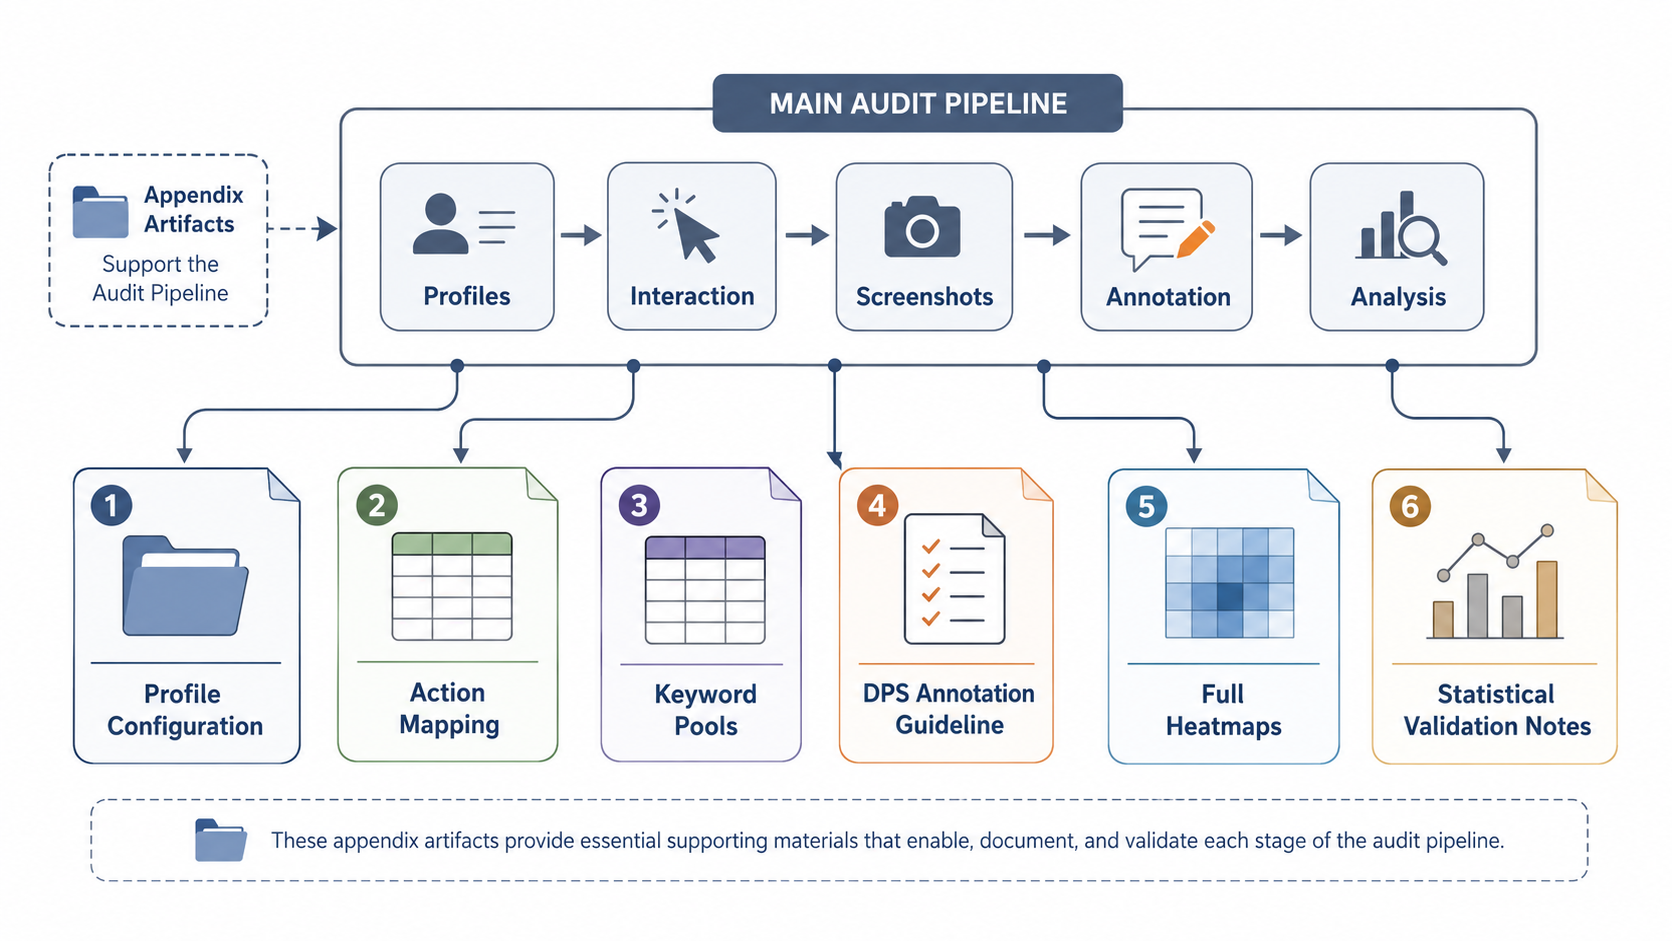
\includegraphics[width=0.95\linewidth]{figures/pictures/appendix_artifact_index.png}
    \caption{Appendix Artifact Index}
    \label{fig:appendix-artifact-index}
\end{figure}

\section{Appendix A: Full Profile Configuration}
\label{app:profile-configuration}

Appendix A reports the full controlled profile configuration used in the audit experiment. Each profile is represented by a behavior distribution over a fixed set of interaction actions. These probabilities are not intended to model any real demographic group. Instead, they define reproducible experimental agents with different interaction tendencies. In this project, the profiles are constructed from controllable interests and behaviors, while demographic attributes are deliberately excluded to reduce ethical and reproducibility concerns.

Table~\ref{tab:profile-behavior-probabilities-appendix} summarizes the behavior probabilities for the three controlled profiles: the high-payment shopping profile, the low-payment browsing profile, and the bargain-hunter profile. The probabilities sum to one within each profile.

The table reports the conceptual action space after collapsing the operational actions used in implementation back into the four high-level categories defined in Chapter~\ref{sec:conceptual-framework}. The mapping from implementation-level actions to conceptual categories is listed in Table~\ref{tab:action-mapping}.

\begin{table}[htbp]
    \centering
    \caption{Behavior probability configuration for controlled user profiles.}
    \label{tab:profile-behavior-probabilities-appendix}
    \begin{tabular}{lccc}
        \toprule
        \textbf{Interaction Action} & 
        \textbf{High-Payment Shopping} & 
        \textbf{Low-Payment Browsing} & 
        \textbf{Bargain Hunter} \\
        \midrule
        Visit homepage & 0.05 & 0.15 & 0.10 \\
        Search keyword & 0.25 & 0.15 & 0.35 \\
        Browse or scroll page & 0.40 & 0.60 & 0.35 \\
        Decision-interface visit & 0.30 & 0.10 & 0.20 \\
        \midrule
        Total & 1.00 & 1.00 & 1.00 \\
        \bottomrule
    \end{tabular}
\end{table}

The high-payment shopping profile is designed to represent an interaction pattern with stronger purchase intent. It searches for high-value products, browses product pages, and more frequently enters decision interfaces such as payment pages, membership pages, or checkout-related screens. The low-payment browsing profile is designed to represent a lower-intent browsing pattern, with more time spent on homepage exploration and general scrolling, and fewer visits to payment-related interfaces. The bargain-hunter profile represents a promotion-sensitive pattern, with stronger attention to discounts, coupons, flash sales, group-buying, and reward mechanisms.

\section{Appendix A.1: Action Mapping}
\label{app:action-mapping}

Table~\ref{tab:action-mapping} maps the implementation-level action set to the four conceptual categories used in the main framework. This mapping is used for analysis and reporting so that fine-grained operational traces can be compared within a shared abstraction.

\begin{table}[htbp]
    \centering
    \caption{Mapping from fine-grained actions to conceptual action categories.}
    \label{tab:action-mapping}
    \small
    \setlength{\tabcolsep}{4pt}
    \renewcommand{\arraystretch}{1.08}
    \begin{tabularx}{\textwidth}{@{}p{3.4cm}p{2.3cm}X@{}}
        \toprule
        \textbf{Fine-grained action} & \textbf{High-level category} & \textbf{Explanation} \\
        \midrule
        \texttt{visit\_homepage} & home & Visits the homepage or returns to the main interface. \\
        \texttt{search\_keyword} & search & Enters a keyword and triggers keyword-based search. \\
        \texttt{browse\_or\_scroll\_page} & browse & Scrolls through or passively explores ordinary content. \\
        \texttt{click\_recommended\_item} & browse & Opens a recommended item during exploratory browsing. \\
        \texttt{like\_or\_favorite} & browse & Expresses lightweight engagement while staying in content exploration. \\
        \texttt{follow\_account} & browse & Follows an account or creator without entering a decision flow. \\
        \texttt{stay\_on\_content} & browse & Remains on content and continues passive exposure to the current feed or page. \\
        \texttt{decision\_interface\_visit} & decision & Enters checkout, subscription, membership, payment, or confirmation interfaces. \\
        \texttt{close\_popup} & home & Dismisses an interruption and returns to the underlying page or main interface. \\
        \texttt{back} & home & Navigates back to the previous page or a higher-level interface. \\
        \bottomrule
    \end{tabularx}
\end{table}

\section{Appendix B: Keyword Pools}
\label{app:keyword-pools}

Appendix B provides the keyword pools used to instantiate the interest component of each controlled profile. In the proposed framework, user interests are modeled as probability distributions over keyword categories. During the interaction process, when the sampled action is the fine-grained \texttt{search\_keyword} action, the system selects a keyword from the corresponding profile-specific keyword pool. This design makes the profile construction controllable and reproducible while still allowing different profiles to generate different interaction traces.

In the operational implementation, this search step corresponds to the fine-grained \texttt{search\_keyword} action, which is mapped back to the conceptual \(\mathrm{search}\) category before analysis.

Table~\ref{tab:keyword-pools} summarizes the keyword categories used by the three profiles.

\begin{table}[htbp]
    \centering
    \caption{Keyword pools for controlled profile construction.}
    \label{tab:keyword-pools}
    \begin{tabular}{lp{9cm}}
        \toprule
        \textbf{Profile} & \textbf{Keyword Categories} \\
        \midrule
        High-payment shopping & 
        High-value goods; premium electronics; luxury skincare; membership services. \\
        \addlinespace
        Low-payment browsing & 
        Daily necessities; casual browsing; snacks; home supplies. \\
        \addlinespace
        Bargain hunter & 
        Discount; coupon; flash sale; group-buy; membership rewards. \\
        \bottomrule
    \end{tabular}
\end{table}

The keyword pools are not intended to exhaustively represent all possible user interests. Rather, they serve as controlled stimuli for auditing whether different interest-behavior configurations are associated with different dark pattern exposure patterns. The implementation files provide the exact keywords used for each category, the sampling probabilities assigned to each keyword group, and examples of generated search instructions.

\section{Appendix C: DPS Annotation Guideline}
\label{app:dps-annotation-guideline}

Appendix C documents the annotation guideline for the seven-dimensional Dark Pattern Score vector, denoted as
\[
DPS = [I, F, P, C, S, N, FA],
\]
where \(I\) refers to Interface Interference, \(F\) to Friction, \(P\) to Pressure, \(C\) to Contextual Deception, \(S\) to Sneaking, \(N\) to Nagging, and \(FA\) to Forced Action. The purpose of this guideline is to improve annotation consistency and make clear how each dimension should be interpreted during screenshot-level labeling.

Table~\ref{tab:dps-guideline} provides the annotation guideline used to interpret the seven DPS dimensions. Detailed examples from collected screenshots are reported in the main DPS chapter where appropriate.

\begin{table}[htbp]
    \centering
    \caption{DPS annotation guideline for mixed numeric exposure scores.}
    \label{tab:dps-guideline}
    \footnotesize
    \setlength{\tabcolsep}{3pt}
    \renewcommand{\arraystretch}{1.06}
    \begin{tabularx}{\textwidth}{@{}p{1.75cm}XXXX@{}}
        \toprule
        \textbf{DPS Dimension} &
        \textbf{Definition} &
        \textbf{Positive Examples} &
        \textbf{Negative Examples} &
        \textbf{Boundary Cases} \\
        \midrule
        Interface Interference \((I)\) &
        Visual or structural design that steers user attention or makes one option more salient than alternatives. &
        A large highlighted ``Buy Now'' button; a visually hidden decline option; misleading button hierarchy. &
        A neutral interface where accept and reject options are equally visible. &
        A visually attractive button is not labeled as interference unless it meaningfully distorts choice visibility or salience. \\
        \addlinespace

        Friction \((F)\) &
        Additional steps, effort, or difficulty imposed on the user when attempting to decline, cancel, close, or avoid an action. &
        Multiple screens required to cancel; difficult unsubscribe path; repeated confirmation before refusal. &
        A single clear cancel or close button. &
        Extra steps may be functional rather than deceptive if they are necessary for security or irreversible actions. \\
        \addlinespace

        Pressure \((P)\) &
        Interface language or timing mechanisms that create urgency, scarcity, social pressure, or emotional pressure. &
        Countdown timers; ``only 2 left'' messages; ``many users are buying now'' prompts; emotionally loaded warnings. &
        Plain factual product information without urgency or emotional manipulation. &
        A real time-limited promotion should be annotated carefully if the interface exaggerates urgency or obscures conditions. \\
        \addlinespace

        Contextual Deception \((C)\) &
        A mismatch between the apparent meaning of an interface element and the actual consequence of interacting with it. &
        A close button that opens another promotion; a misleading checkbox; a button label that hides subscription consequences. &
        A clearly labeled button whose result matches user expectation. &
        Ambiguous icons should be annotated only when the surrounding context suggests a misleading or deceptive interpretation. \\
        \addlinespace

        Sneaking \((S)\) &
        Hidden or delayed disclosure of costs, conditions, subscriptions, add-ons, or data-related consequences. &
        Hidden fees added near checkout; preselected add-ons; unclear membership renewal terms. &
        Fully disclosed price, fee, and subscription information before user commitment. &
        Additional charges are not labeled as sneaking if they are clearly disclosed before the decision point. \\
        \addlinespace

        Nagging \((N)\) &
        Repeated interruptions or prompts that ask the user to perform an action unrelated to the immediate task. &
        Repeated pop-ups for membership, notification permission, app rating, or promotion after dismissal. &
        A single relevant reminder that does not interrupt the task flow. &
        Repetition should be considered in relation to interaction history; a single prompt may become nagging if it repeatedly reappears after refusal. \\
        \addlinespace

        Forced Action \((FA)\) &
        A design that requires the user to perform an additional action, registration, permission grant, or commitment before continuing. &
        Mandatory login before browsing; forced app permission; required membership prompt before accessing core content. &
        Optional login or permission request that can be skipped without blocking the task. &
        Some forced actions may be functionally necessary, such as payment authentication; these should be distinguished from unnecessary coercive barriers. \\
        \bottomrule
    \end{tabularx}
\end{table}

The scoring scheme combines binary indicators and numeric exposure scores. Pressure, Contextual Deception, Sneaking, and Forced Action are typically treated as binary labels in the present dataset. Interface Interference, Friction, and Nagging may use ordinal levels or counts when the annotation protocol distinguishes weak from strong exposure, additional effort, or repeated interruption. Occurrence-rate analysis uses \(D_i>0\), while intensity analysis uses raw score means.

\section{Appendix D: Full Heatmaps}
\label{app:full-heatmaps}

Appendix D provides the complete set of DPS heatmaps for all audited applications and profiles. In the main report, only representative heatmaps are shown to illustrate the most important exposure patterns. The appendix includes the full visualization set so that readers can inspect the distribution of dark pattern exposure across the complete experimental scope.

Each heatmap uses the DPS dimensions as one axis and either applications, profiles, or application categories as the other axis, depending on the visualization design. These heatmaps are intended to support the main finding that different profiles show different exposure patterns. They also allow readers to identify which DPS dimensions are more prominent in particular app categories.

\begin{figure}[htbp]
    \centering
    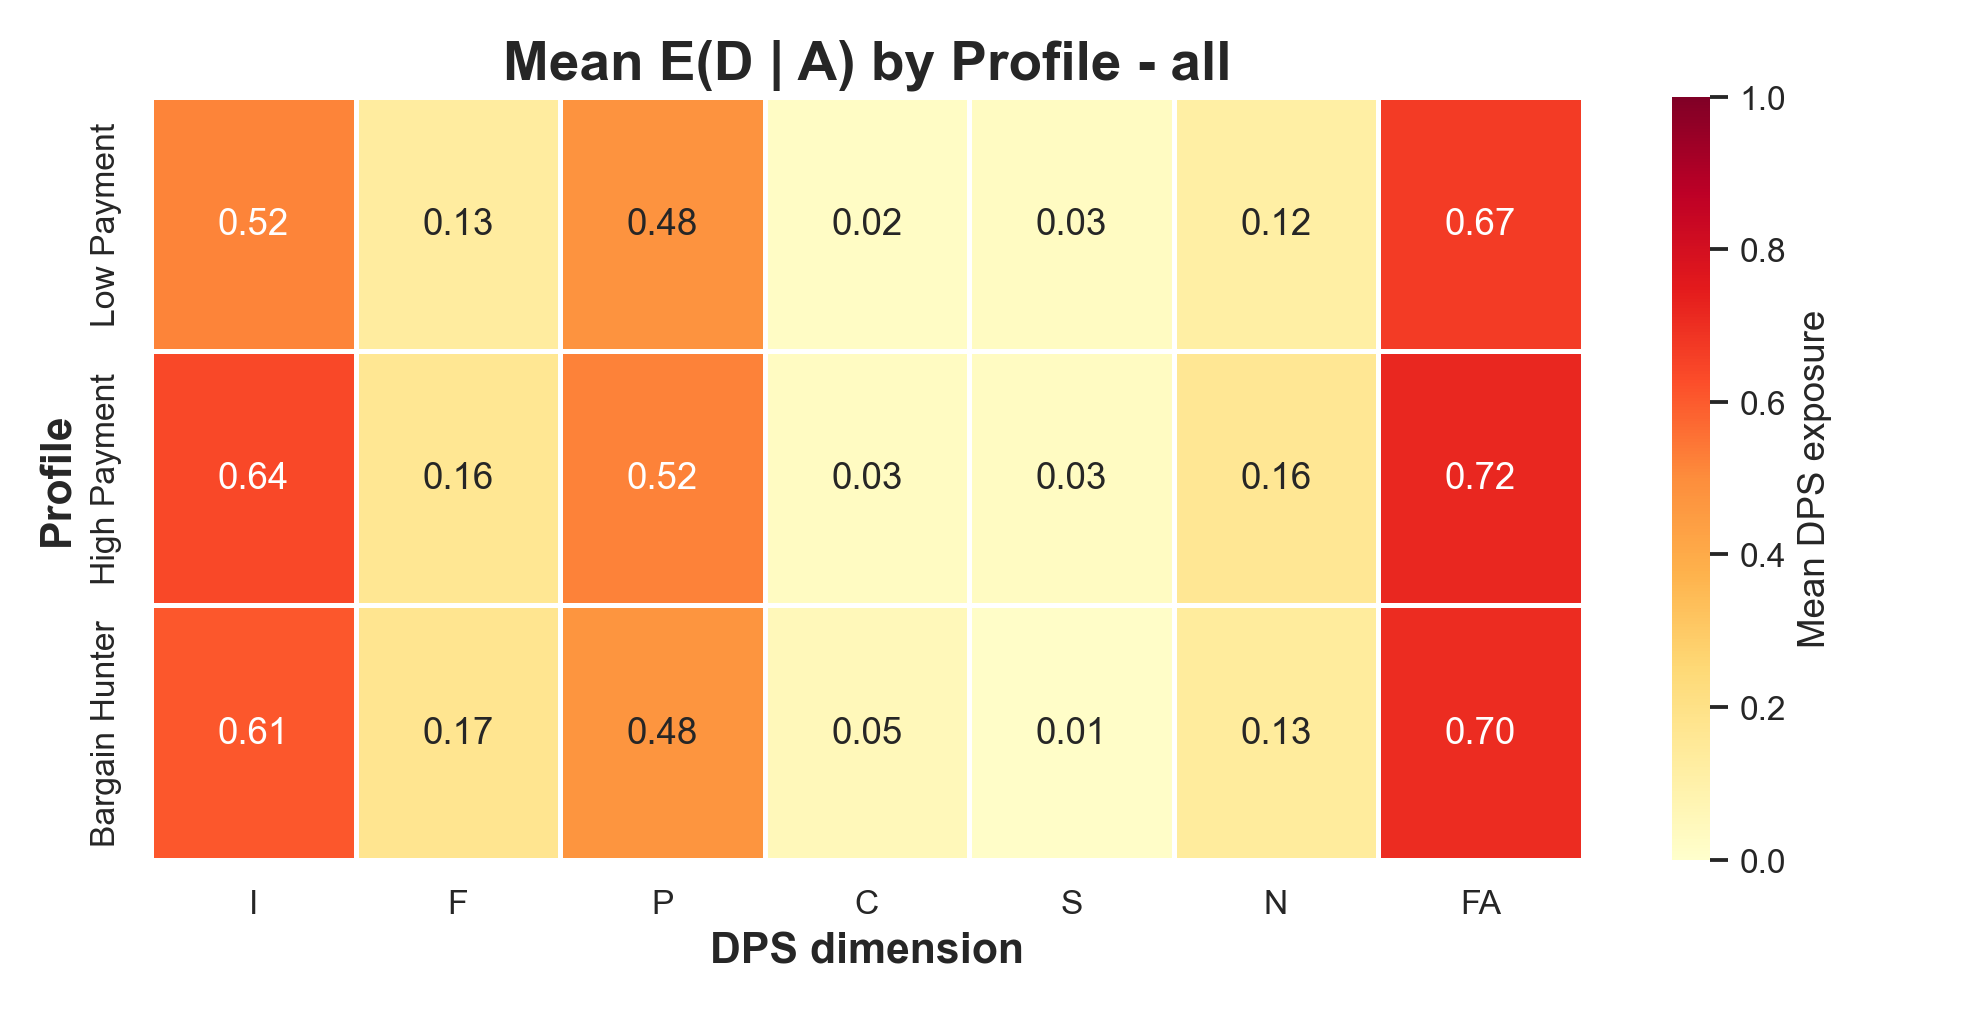
\includegraphics[width=0.95\linewidth]{figures/statistics/heatmap_mean_exposure_all.png}
    \caption{Complete raw DPS intensity mean heatmap for all applications and controlled profiles.}
    \label{fig:full-heatmap-all}
\end{figure}

\begin{figure}[htbp]
    \centering
    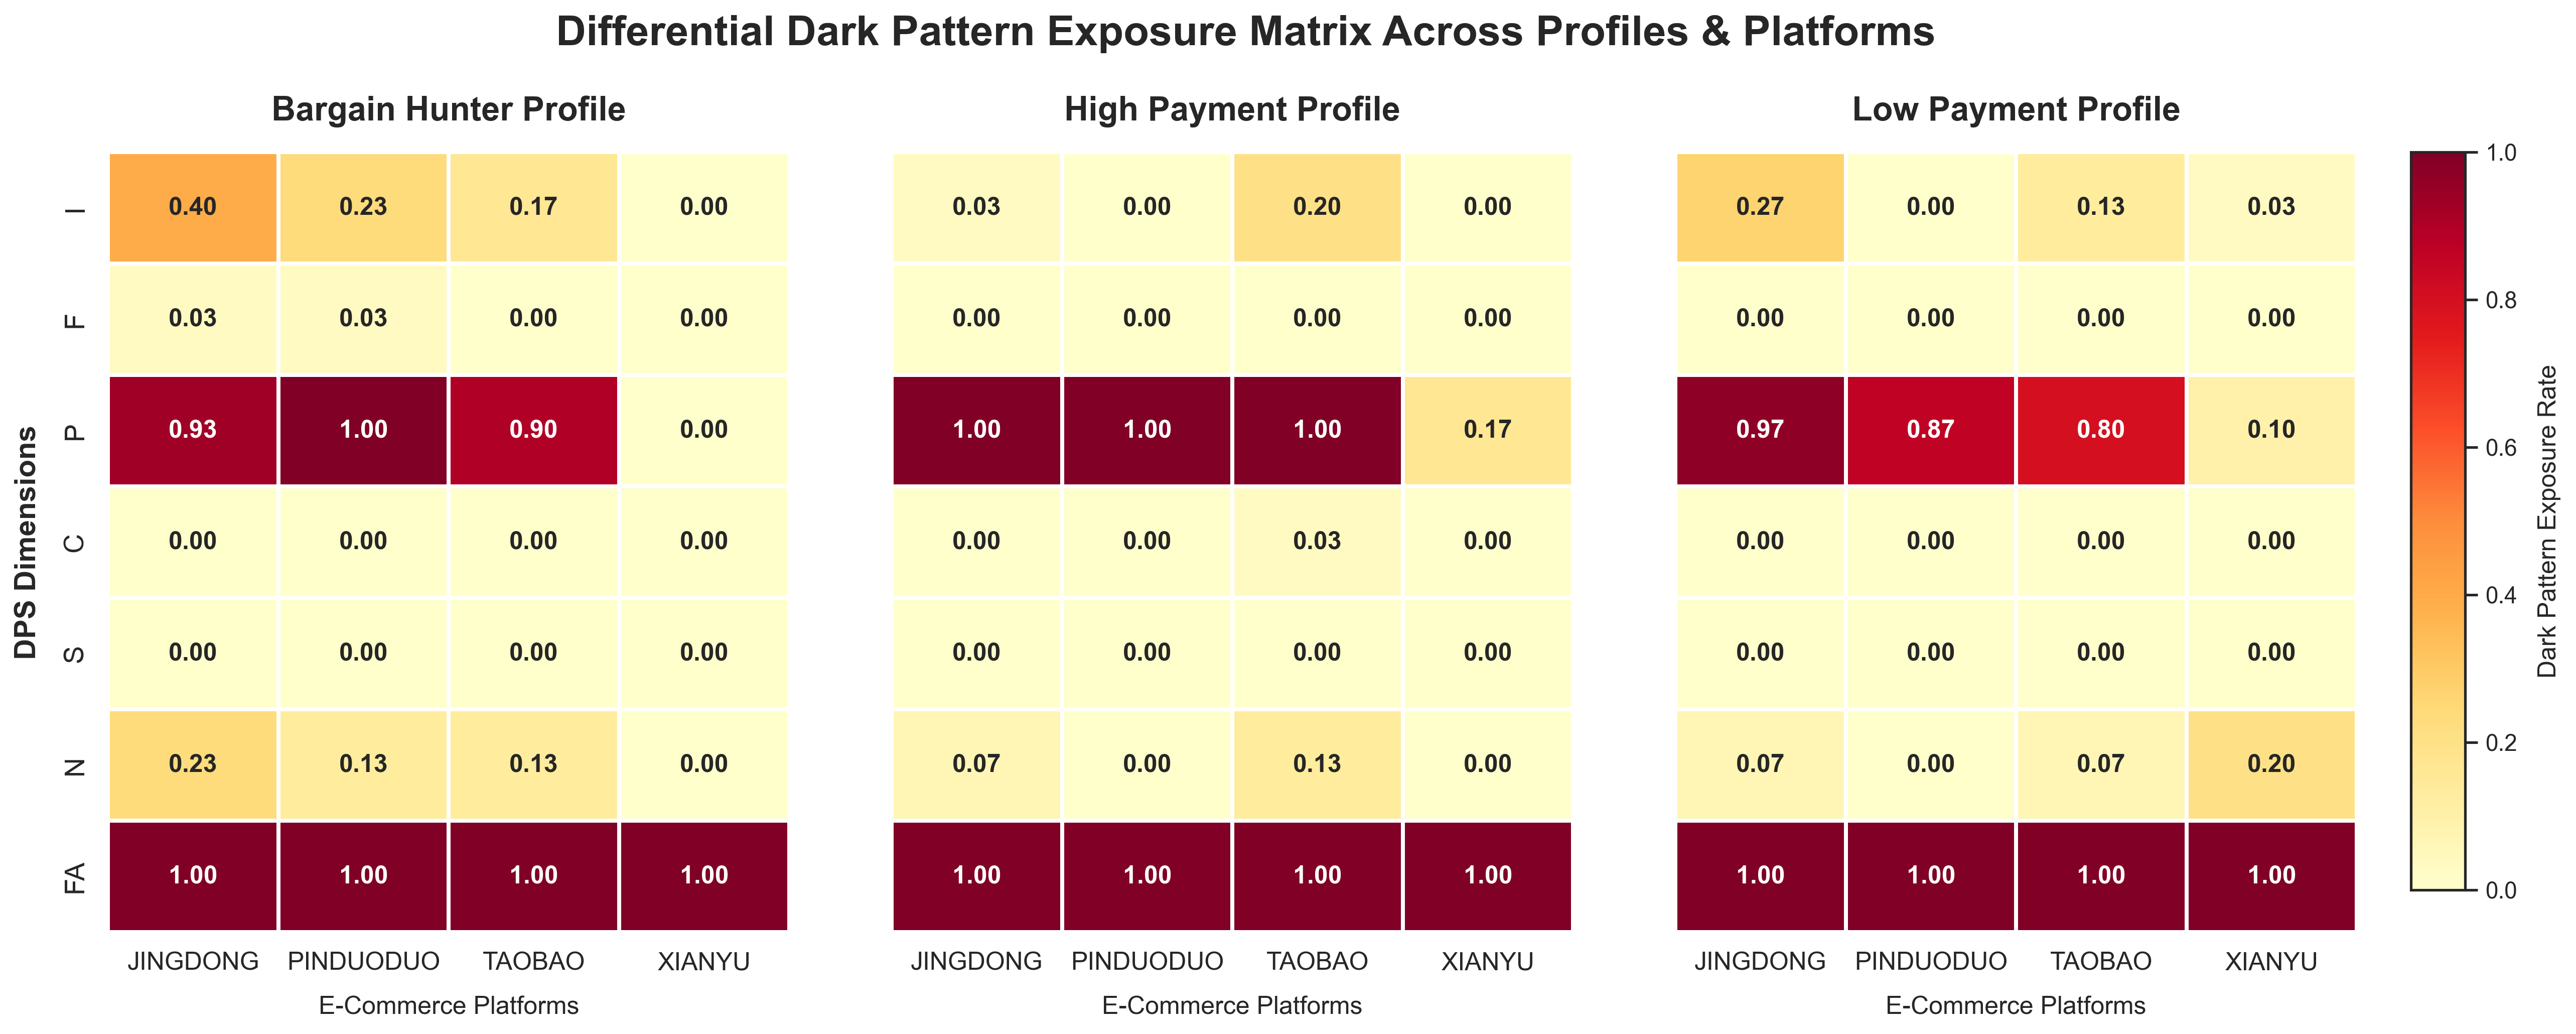
\includegraphics[width=0.95\linewidth]{figures/heatmap_shopping.png}
    \caption{Detailed raw DPS intensity heatmap for shopping applications.}
    \label{fig:heatmap-shopping-detail}
\end{figure}

\begin{figure}[htbp]
    \centering
    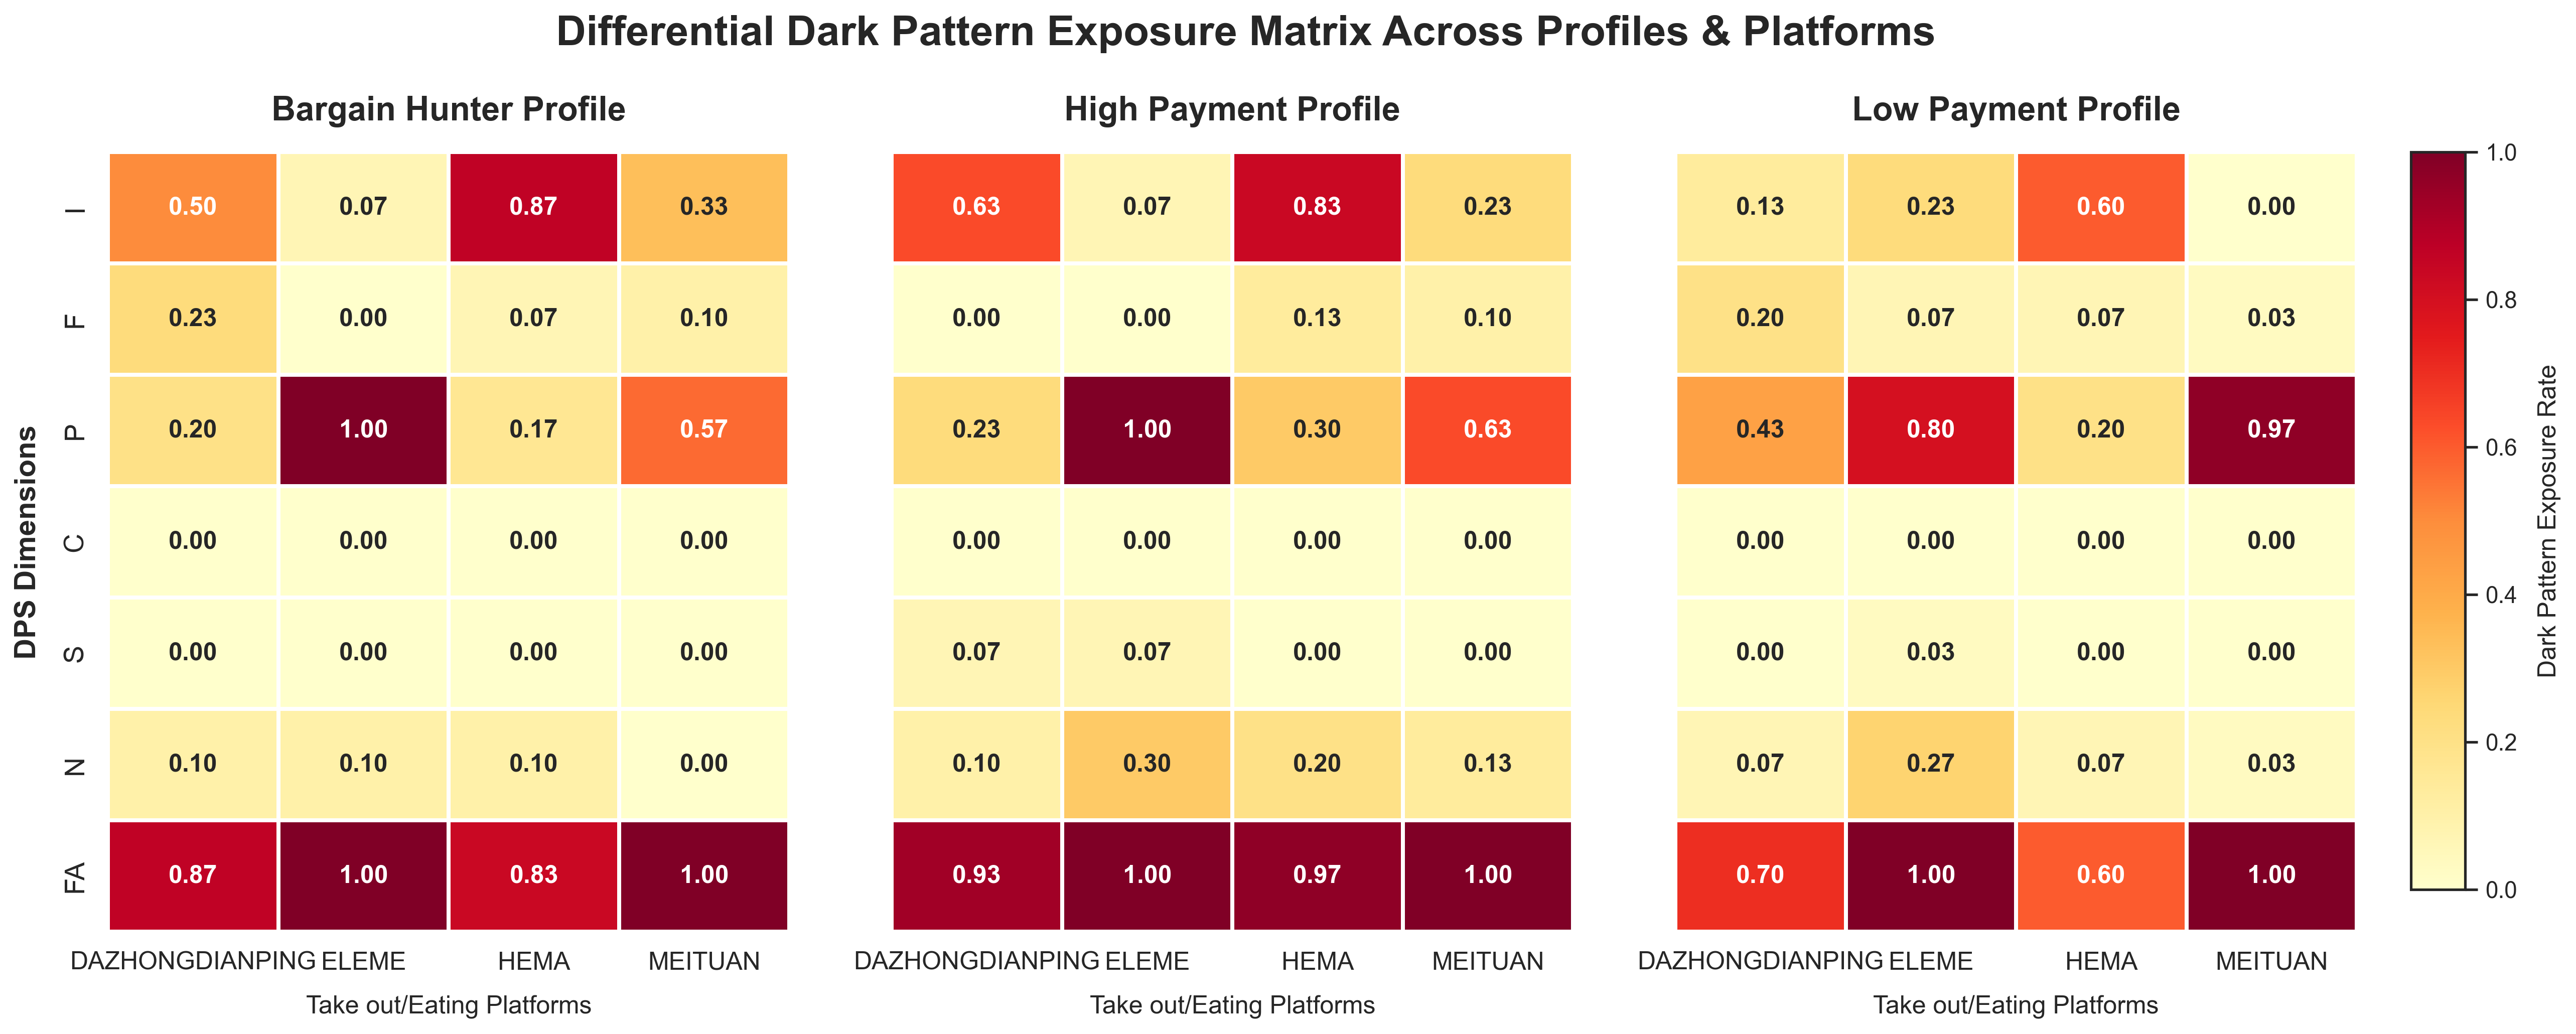
\includegraphics[width=0.95\linewidth]{figures/heatmap_eating.png}
    \caption{Detailed raw DPS intensity heatmap for food-delivery and eating-related applications.}
    \label{fig:heatmap-eating-detail}
\end{figure}

\begin{figure}[htbp]
    \centering
    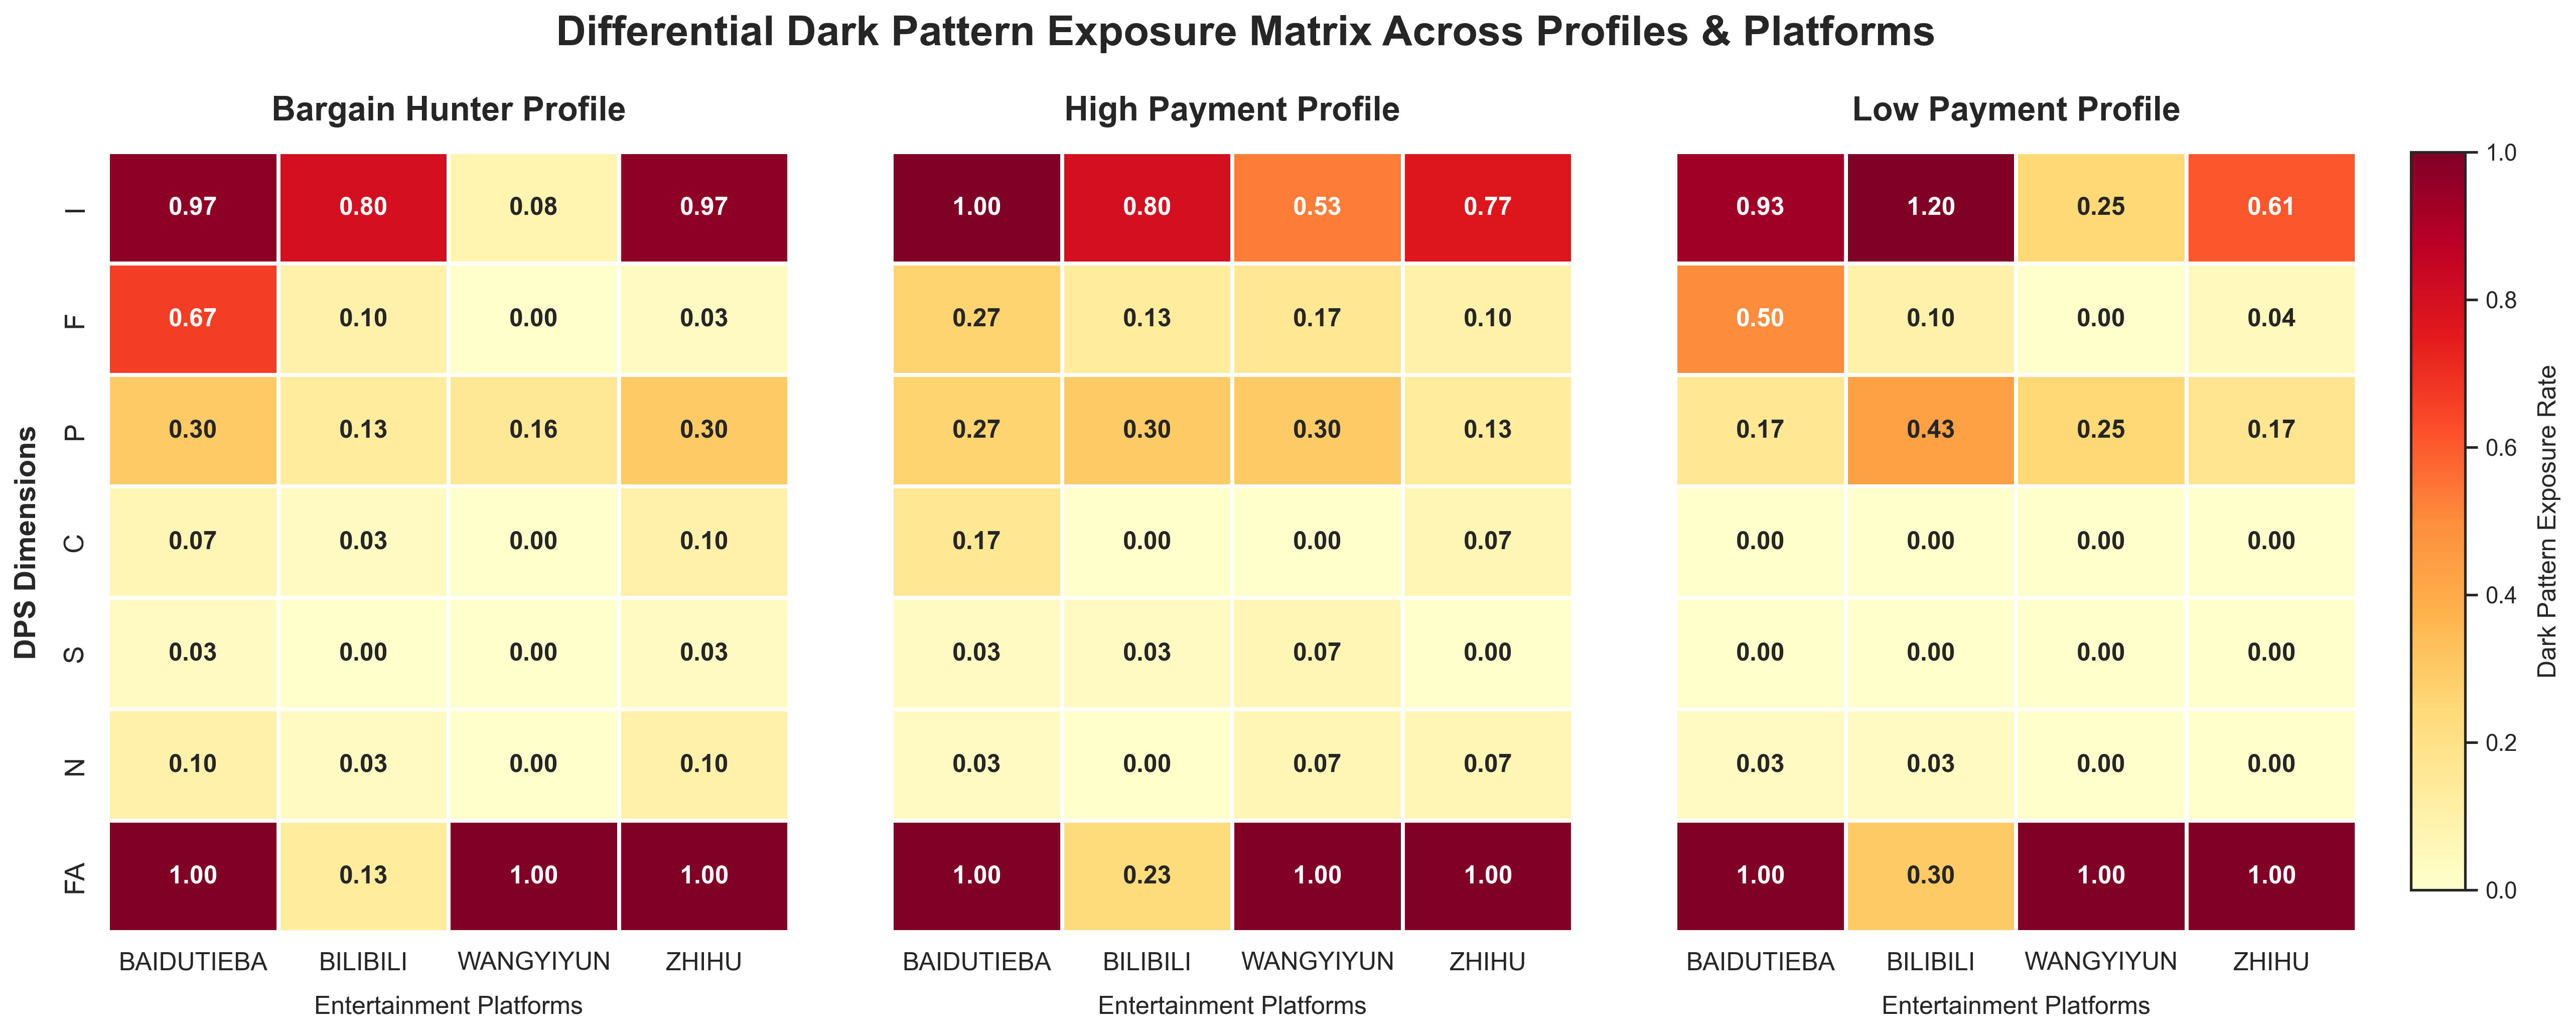
\includegraphics[width=0.95\linewidth]{figures/heatmap_entertainment.png}
    \caption{Detailed raw DPS intensity heatmap for entertainment applications.}
    \label{fig:heatmap-entertainment-detail}
\end{figure}

\begin{figure}[htbp]
    \centering
    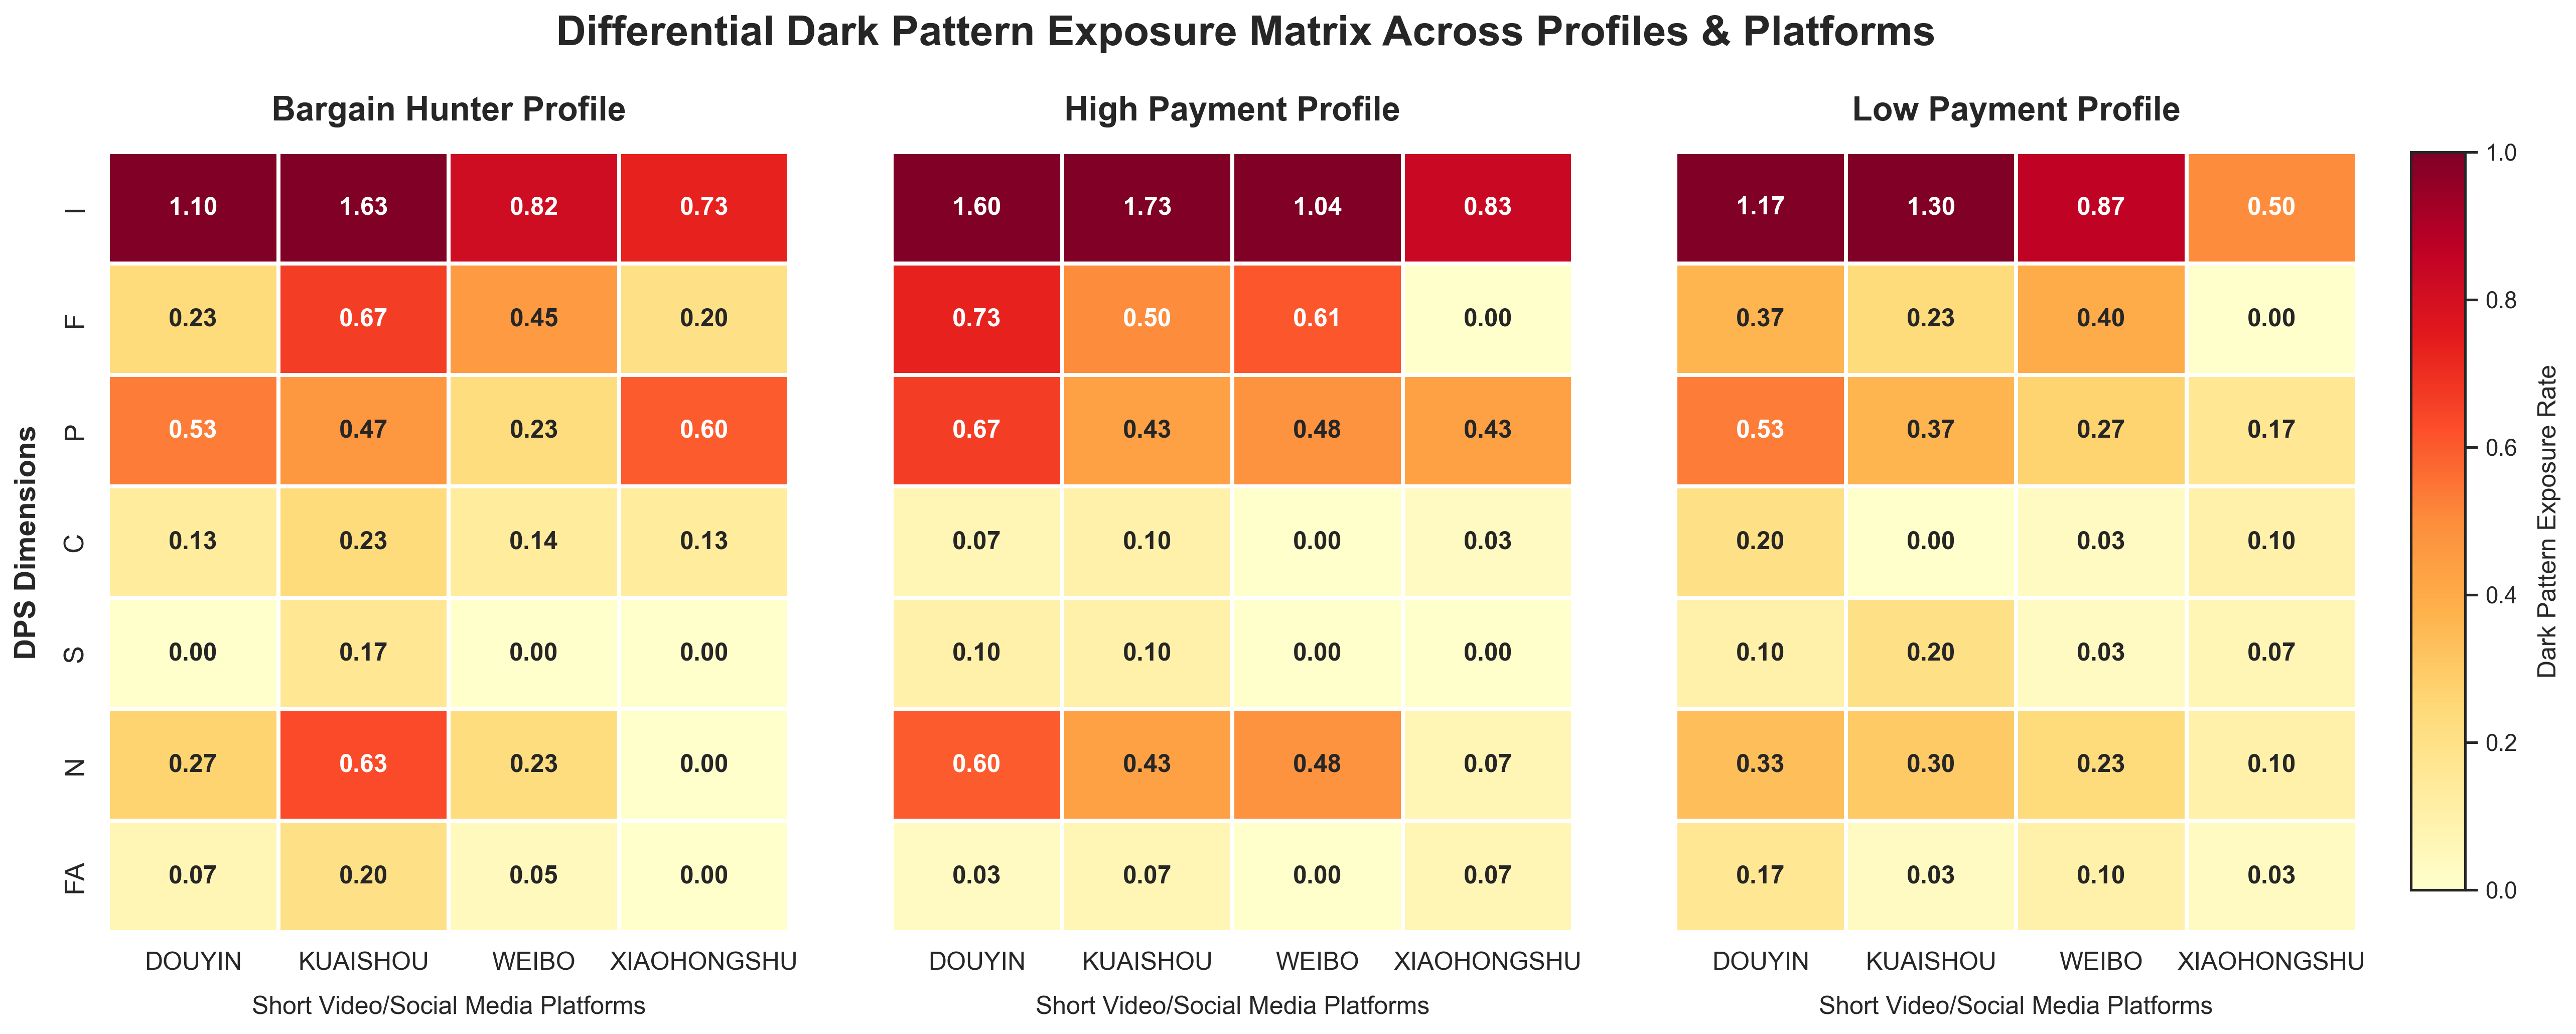
\includegraphics[width=0.95\linewidth]{figures/heatmap_social.png}
    \caption{Detailed raw DPS intensity heatmap for social applications.}
    \label{fig:heatmap-social-detail}
\end{figure}

The captions in this appendix describe what each heatmap represents without restating unsupported causal claims. The text uses careful language such as ``the heatmap indicates higher observed exposure'' or ``the pattern suggests profile-associated differences in exposure.''

\section{Appendix E: Statistical Visualization Set}
\label{app:statistical-visualizations}

Appendix E includes the complete statistical visualization set currently exported by the analysis pipeline. These figures complement the main report by showing q-value patterns, permutation-test summaries, observed L1 distances, Cramér's \(V\) association strengths, and running mean convergence curves.

For a DPS dimension \(d\), the running mean after \(t\) interaction steps can be written as
\[
\bar{D}_{A,d}^{(t)} = \frac{1}{t}\sum_{\tau=1}^{t} D_{A,d}^{(\tau)},
\]
where \(A\) denotes the controlled profile and \(D_{A,d}^{(\tau)}\) denotes the observed DPS label for dimension \(d\) at step \(\tau\).

\subsection{Running Mean Convergence Curves}
\label{app:running-mean-curves}

The following running mean convergence curves collect the full set of exported line plots from the analysis pipeline. They are grouped by application category and arranged in four columns so that several curves appear on each row.

\newcommand{\curvecell}[1]{%
    \begin{minipage}[t]{0.24\textwidth}
        \centering
        \includegraphics[width=\linewidth]{#1}
    \end{minipage}%
}

\subsubsection{Shopping}
\noindent
\curvecell{figures/statistics/curves_shopping/curve_E_bargain_hunter_jingdong_shopping.png}\hfill
\curvecell{figures/statistics/curves_shopping/curve_E_bargain_hunter_pinduoduo_shopping.png}\hfill
\curvecell{figures/statistics/curves_shopping/curve_E_bargain_hunter_taobao_shopping.png}\hfill
\curvecell{figures/statistics/curves_shopping/curve_E_bargain_hunter_xianyu_shopping.png}

\par\medskip

\noindent
\curvecell{figures/statistics/curves_shopping/curve_E_high_payment_shopping_jingdong_shopping.png}\hfill
\curvecell{figures/statistics/curves_shopping/curve_E_high_payment_shopping_pinduoduo_shopping.png}\hfill
\curvecell{figures/statistics/curves_shopping/curve_E_high_payment_shopping_taobao_shopping.png}\hfill
\curvecell{figures/statistics/curves_shopping/curve_E_high_payment_shopping_xianyu_shopping.png}

\par\medskip

\noindent
\curvecell{figures/statistics/curves_shopping/curve_E_low_payment_browsing_jingdong_shopping.png}\hfill
\curvecell{figures/statistics/curves_shopping/curve_E_low_payment_browsing_pinduoduo_shopping.png}\hfill
\curvecell{figures/statistics/curves_shopping/curve_E_low_payment_browsing_taobao_shopping.png}\hfill
\curvecell{figures/statistics/curves_shopping/curve_E_low_payment_browsing_xianyu_shopping.png}

\par\medskip

\subsubsection{Eating}
\noindent
\curvecell{figures/statistics/curves_eating/curve_E_bargain_hunter_DaZhongDianPing_eating.png}\hfill
\curvecell{figures/statistics/curves_eating/curve_E_bargain_hunter_ELeMe_eating.png}\hfill
\curvecell{figures/statistics/curves_eating/curve_E_bargain_hunter_HeMa_eating.png}\hfill
\curvecell{figures/statistics/curves_eating/curve_E_bargain_hunter_MeiTuan_eating.png}

\par\medskip

\noindent
\curvecell{figures/statistics/curves_eating/curve_E_high_payment_shopping_DaZhongDianPing_eating.png}\hfill
\curvecell{figures/statistics/curves_eating/curve_E_high_payment_shopping_ELeMe_eating.png}\hfill
\curvecell{figures/statistics/curves_eating/curve_E_high_payment_shopping_HeMa_eating.png}\hfill
\curvecell{figures/statistics/curves_eating/curve_E_high_payment_shopping_MeiTuan_eating.png}

\par\medskip

\noindent
\curvecell{figures/statistics/curves_eating/curve_E_low_payment_browsing_DaZhongDianPing_eating.png}\hfill
\curvecell{figures/statistics/curves_eating/curve_E_low_payment_browsing_ELeMe_eating.png}\hfill
\curvecell{figures/statistics/curves_eating/curve_E_low_payment_browsing_HeMa_eating.png}\hfill
\curvecell{figures/statistics/curves_eating/curve_E_low_payment_browsing_MeiTuan_eating.png}

\par\medskip

\subsubsection{Entertainment}
\noindent
\curvecell{figures/statistics/curves_entertainment/curve_E_bargain_hunter_BaiDuTieBa_entertainment.png}\hfill
\curvecell{figures/statistics/curves_entertainment/curve_E_bargain_hunter_BiliBili_entertainment.png}\hfill
\curvecell{figures/statistics/curves_entertainment/curve_E_bargain_hunter_WangYiYun_entertainment.png}\hfill
\curvecell{figures/statistics/curves_entertainment/curve_E_bargain_hunter_ZhiHu_entertainment.png}

\par\medskip

\noindent
\curvecell{figures/statistics/curves_entertainment/curve_E_high_payment_shopping_BaiDuTieBa_entertainment.png}\hfill
\curvecell{figures/statistics/curves_entertainment/curve_E_high_payment_shopping_BiliBili_entertainment.png}\hfill
\curvecell{figures/statistics/curves_entertainment/curve_E_high_payment_shopping_WangYiYun_entertainment.png}\hfill
\curvecell{figures/statistics/curves_entertainment/curve_E_high_payment_shopping_ZhiHu_entertainment.png}

\par\medskip

\noindent
\curvecell{figures/statistics/curves_entertainment/curve_E_low_payment_browsing_BaiDuTieBa_entertainment.png}\hfill
\curvecell{figures/statistics/curves_entertainment/curve_E_low_payment_browsing_BiliBili_entertainment.png}\hfill
\curvecell{figures/statistics/curves_entertainment/curve_E_low_payment_browsing_WangYiYun_entertainment.png}\hfill
\curvecell{figures/statistics/curves_entertainment/curve_E_low_payment_browsing_ZhiHu_entertainment.png}

\par\medskip

\subsubsection{Social}
\noindent
\curvecell{figures/statistics/curves_social/curve_E_bargain_hunter_DouYin_social.png}\hfill
\curvecell{figures/statistics/curves_social/curve_E_bargain_hunter_KuaiShou_social.png}\hfill
\curvecell{figures/statistics/curves_social/curve_E_bargain_hunter_WeiBo_social.png}\hfill
\curvecell{figures/statistics/curves_social/curve_E_bargain_hunter_XiaoHongShu_social.png}

\par\medskip

\noindent
\curvecell{figures/statistics/curves_social/curve_E_high_payment_shopping_DouYin_social.png}\hfill
\curvecell{figures/statistics/curves_social/curve_E_high_payment_shopping_KuaiShou_social.png}\hfill
\curvecell{figures/statistics/curves_social/curve_E_high_payment_shopping_WeiBo_social.png}\hfill
\curvecell{figures/statistics/curves_social/curve_E_high_payment_shopping_XiaoHongShu_social.png}

\par\medskip

\noindent
\curvecell{figures/statistics/curves_social/curve_E_low_payment_browsing_DouYin_social.png}\hfill
\curvecell{figures/statistics/curves_social/curve_E_low_payment_browsing_KuaiShou_social.png}\hfill
\curvecell{figures/statistics/curves_social/curve_E_low_payment_browsing_WeiBo_social.png}\hfill
\curvecell{figures/statistics/curves_social/curve_E_low_payment_browsing_XiaoHongShu_social.png}

\par\medskip


\begin{figure}[htbp]
    \centering
    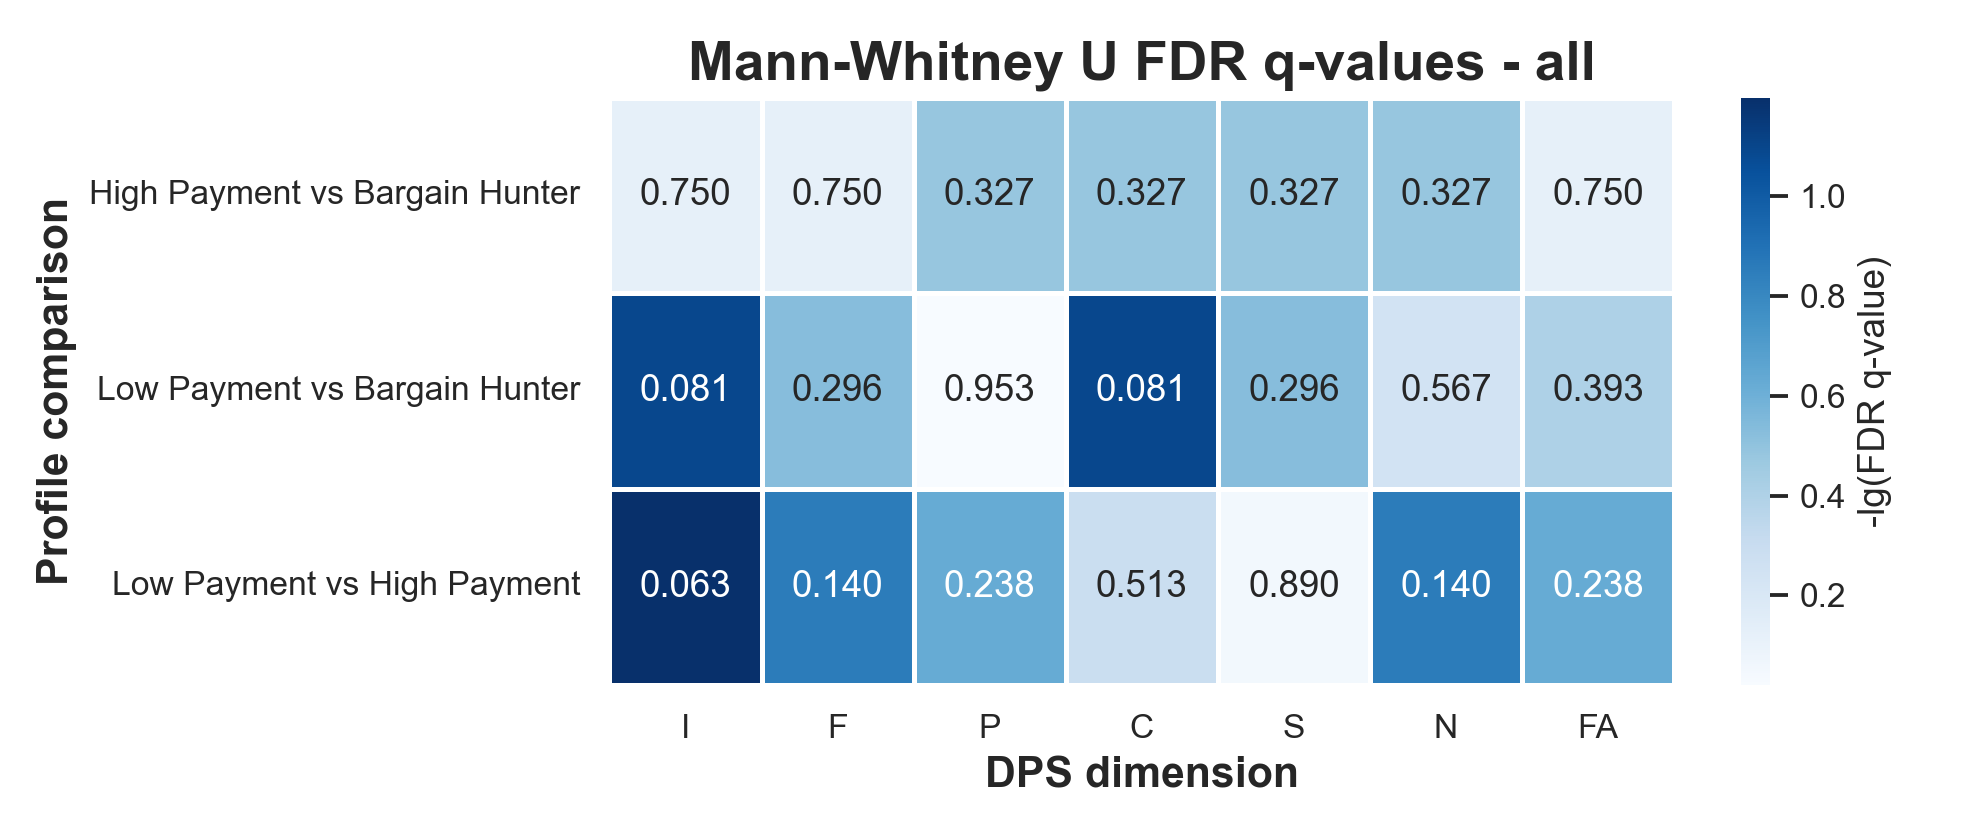
\includegraphics[width=0.95\linewidth]{figures/statistics/mannwhitney_qvalue_heatmap_all.png}
    \caption{Mann-Whitney U BH FDR q-value heatmap for raw DPS intensity comparisons across all audited applications.}
    \label{fig:qvalue-all-appendix}
\end{figure}

\begin{figure}[htbp]
    \centering
    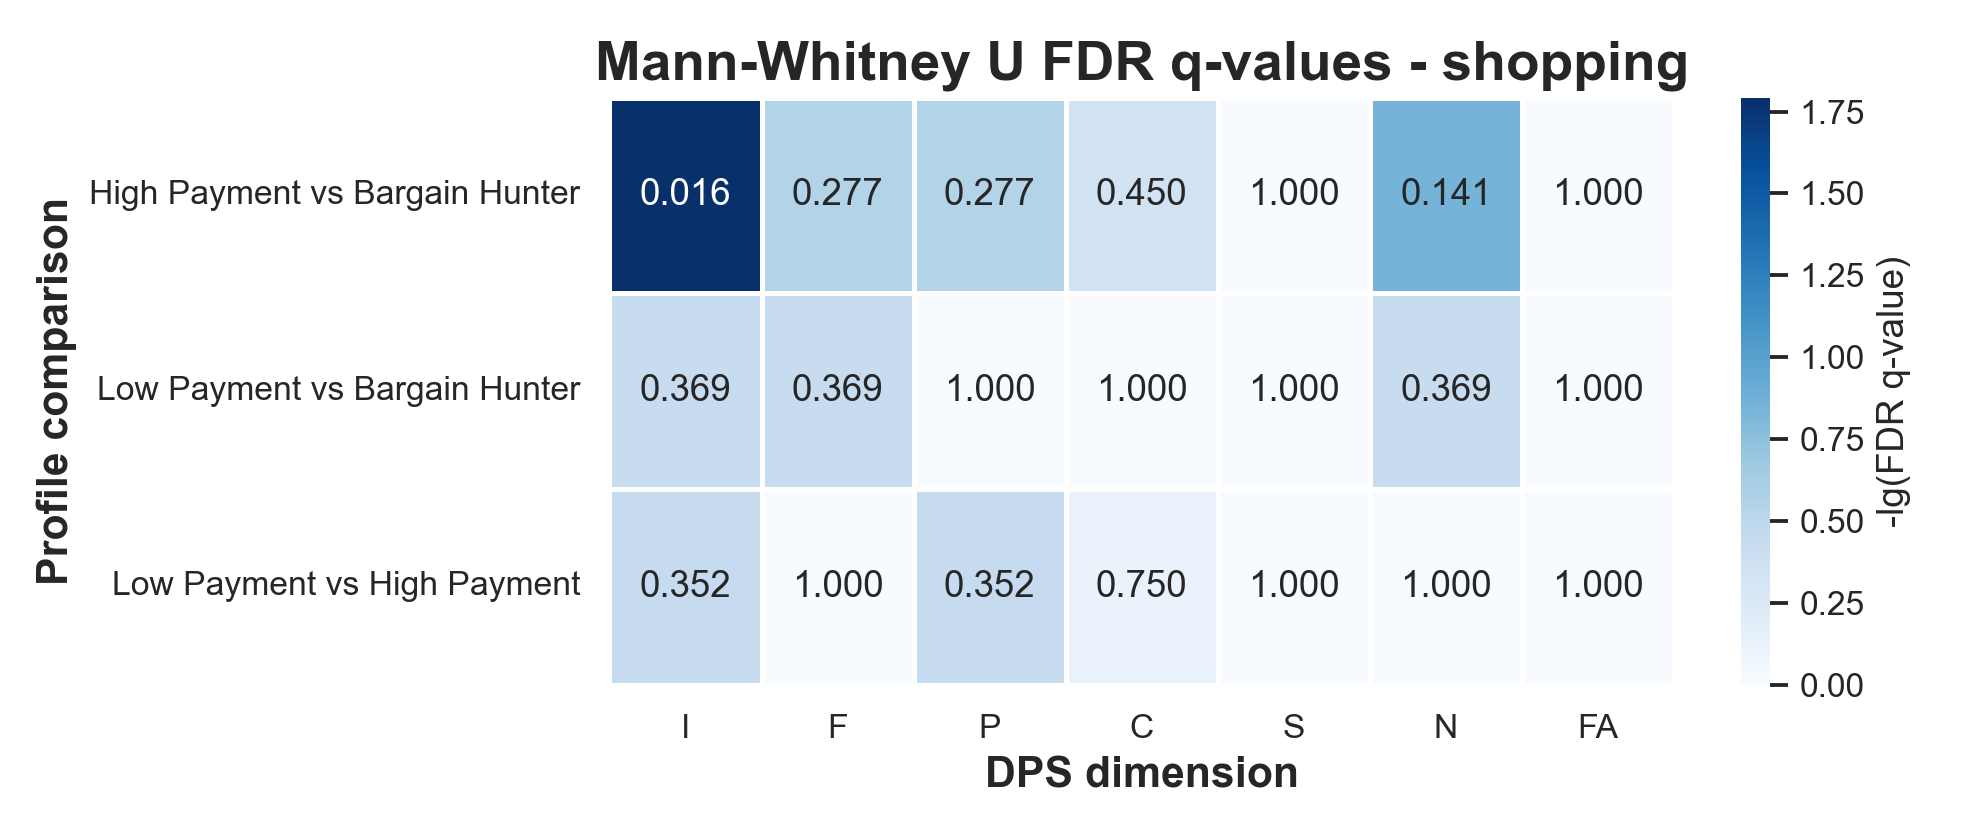
\includegraphics[width=0.95\linewidth]{figures/statistics/mannwhitney_qvalue_heatmap_shopping.png}
    \caption{Mann-Whitney U BH FDR q-value heatmap for raw DPS intensity comparisons in shopping applications.}
    \label{fig:qvalue-shopping}
\end{figure}

\begin{figure}[htbp]
    \centering
    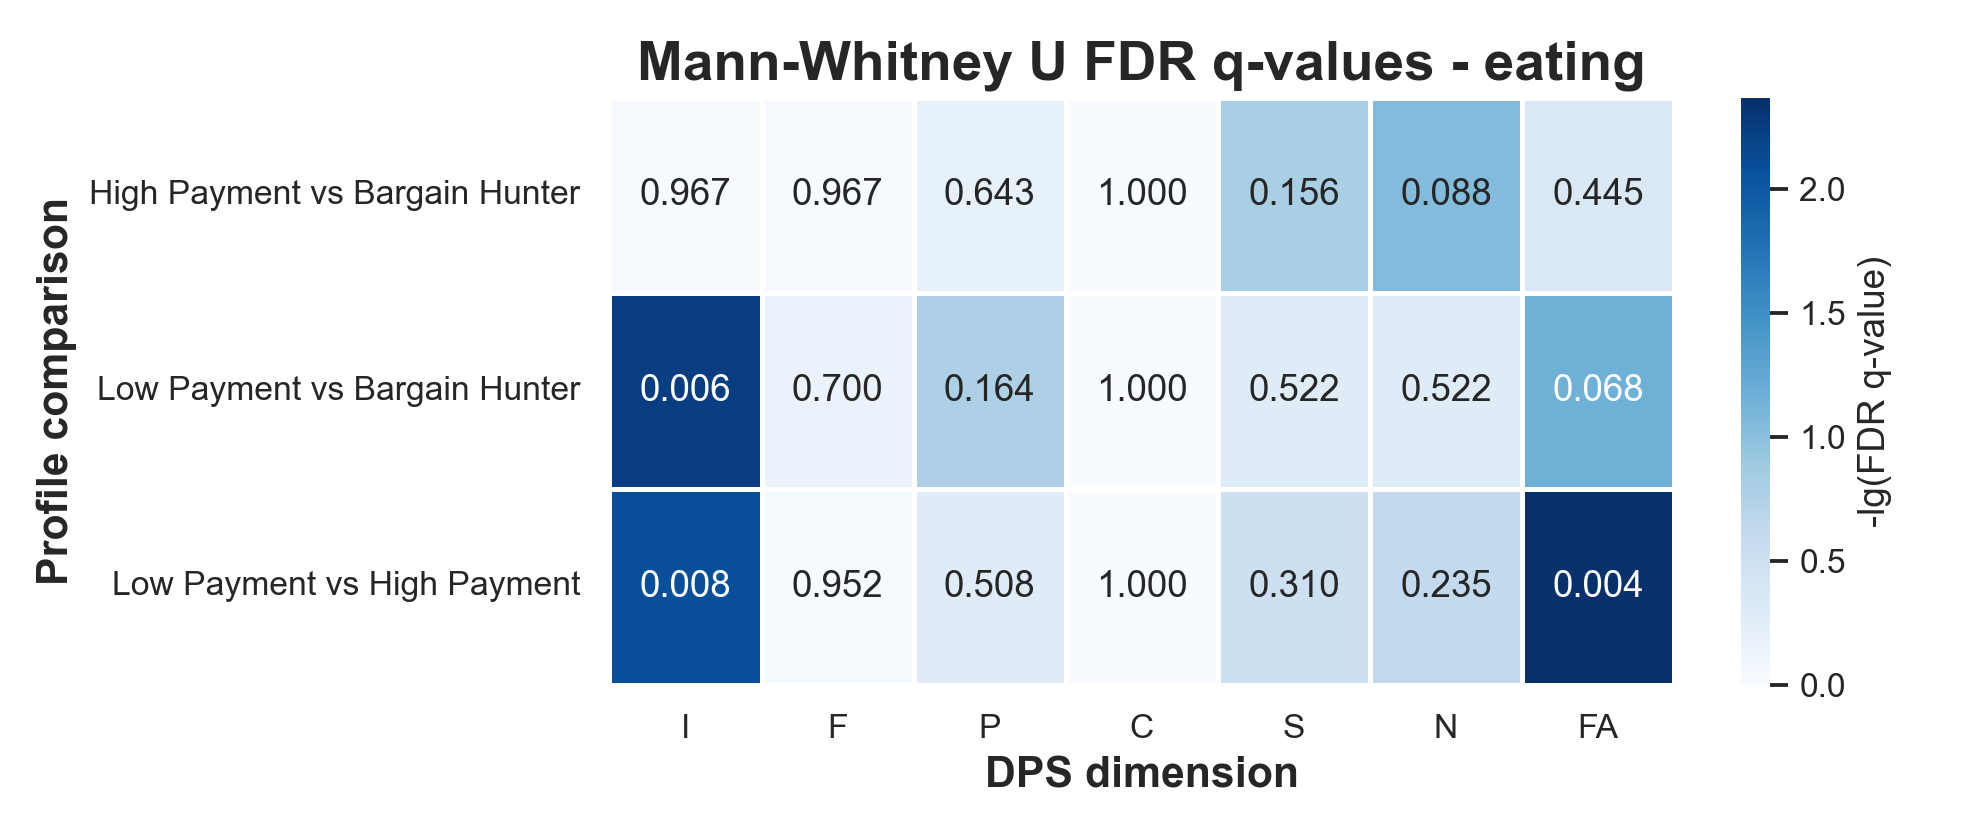
\includegraphics[width=0.95\linewidth]{figures/statistics/mannwhitney_qvalue_heatmap_eating.png}
    \caption{Mann-Whitney U BH FDR q-value heatmap for raw DPS intensity comparisons in food-delivery and eating-related applications.}
    \label{fig:qvalue-eating}
\end{figure}

\begin{figure}[htbp]
    \centering
    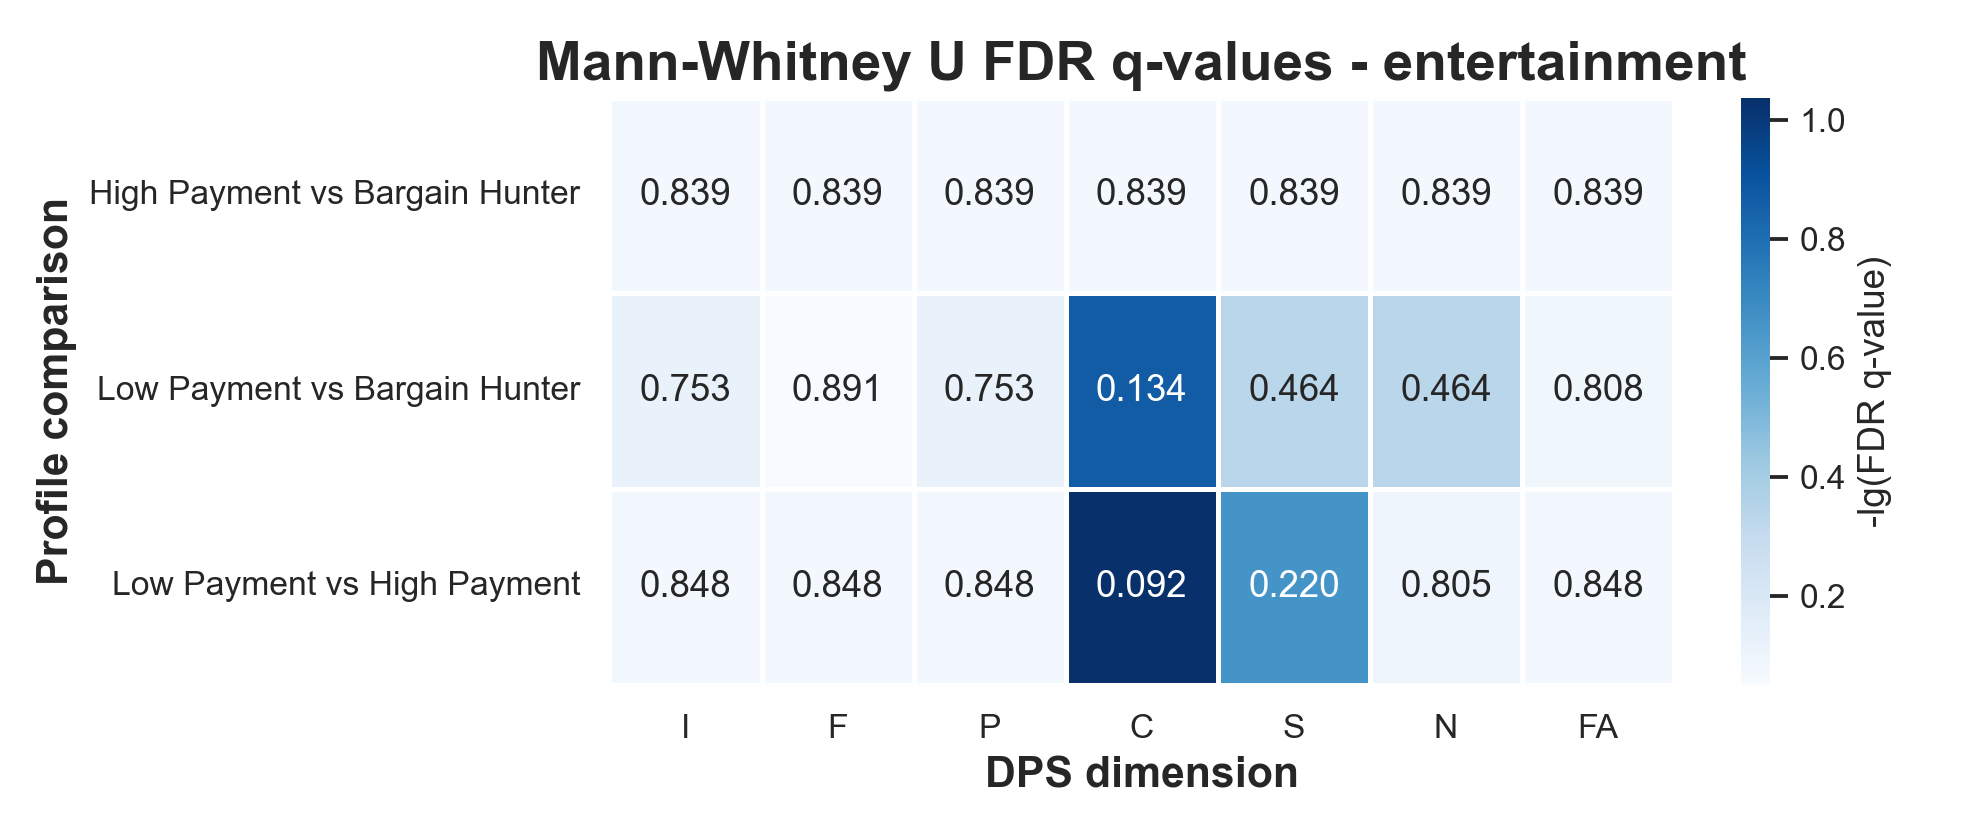
\includegraphics[width=0.95\linewidth]{figures/statistics/mannwhitney_qvalue_heatmap_entertainment.png}
    \caption{Mann-Whitney U BH FDR q-value heatmap for raw DPS intensity comparisons in entertainment applications.}
    \label{fig:qvalue-entertainment}
\end{figure}

\begin{figure}[htbp]
    \centering
    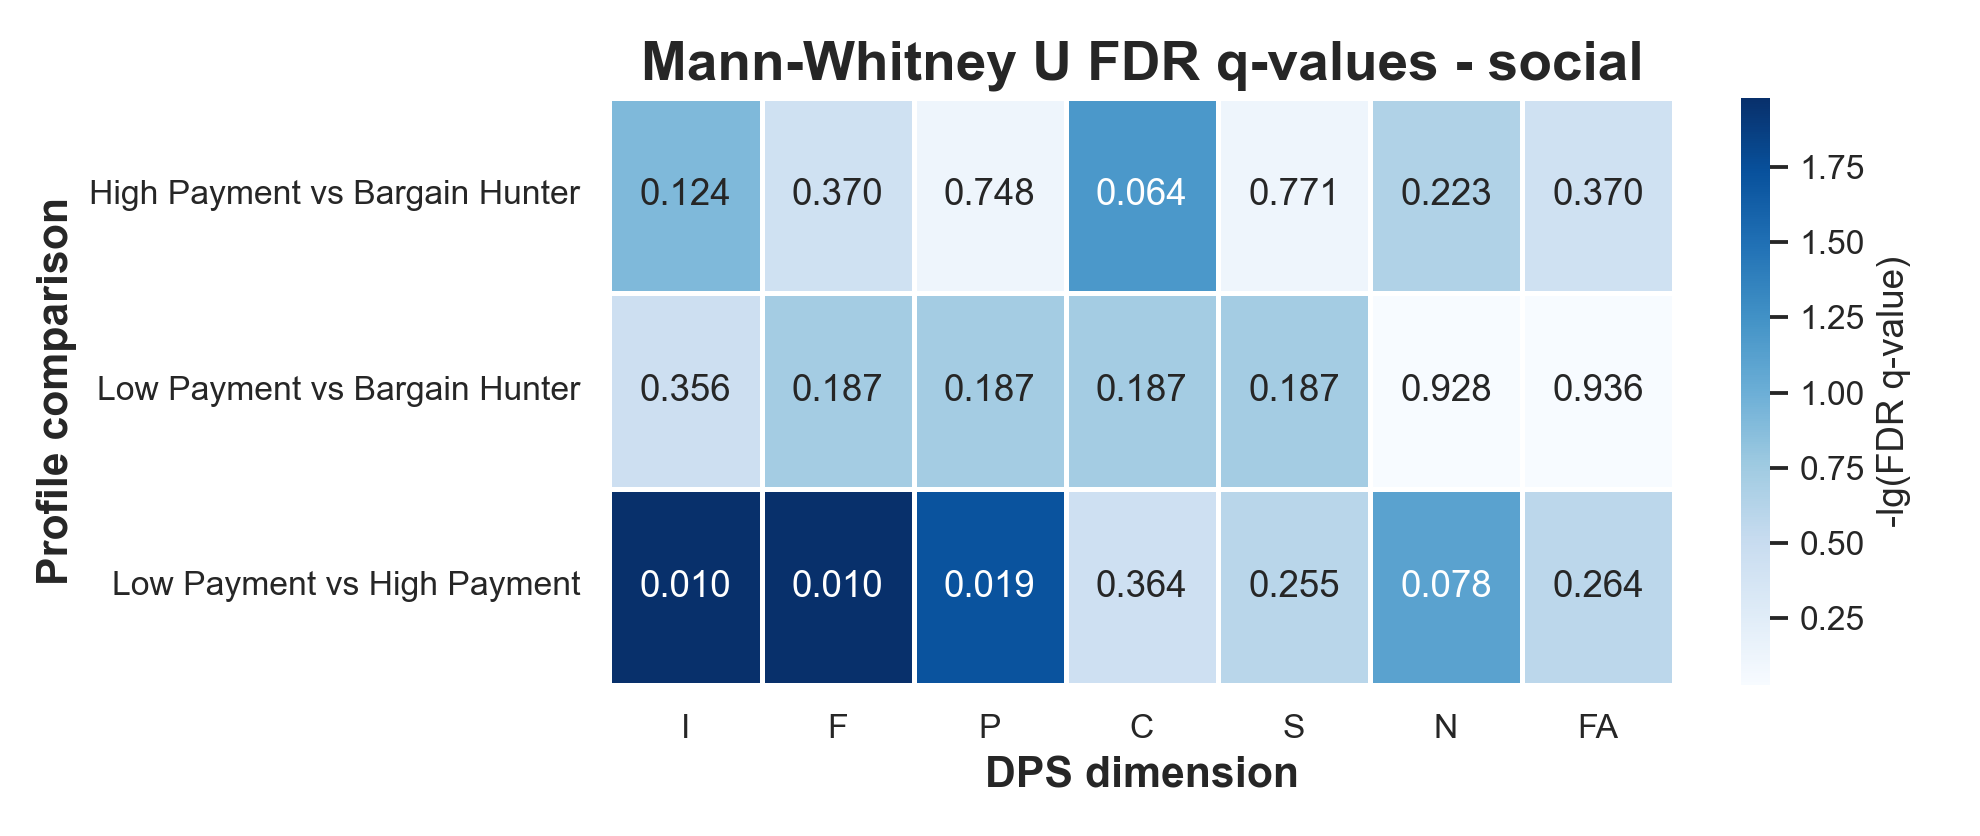
\includegraphics[width=0.95\linewidth]{figures/statistics/mannwhitney_qvalue_heatmap_social.png}
    \caption{Mann-Whitney U BH FDR q-value heatmap for raw DPS intensity comparisons in social applications.}
    \label{fig:qvalue-social}
\end{figure}

\begin{figure}[htbp]
    \centering
    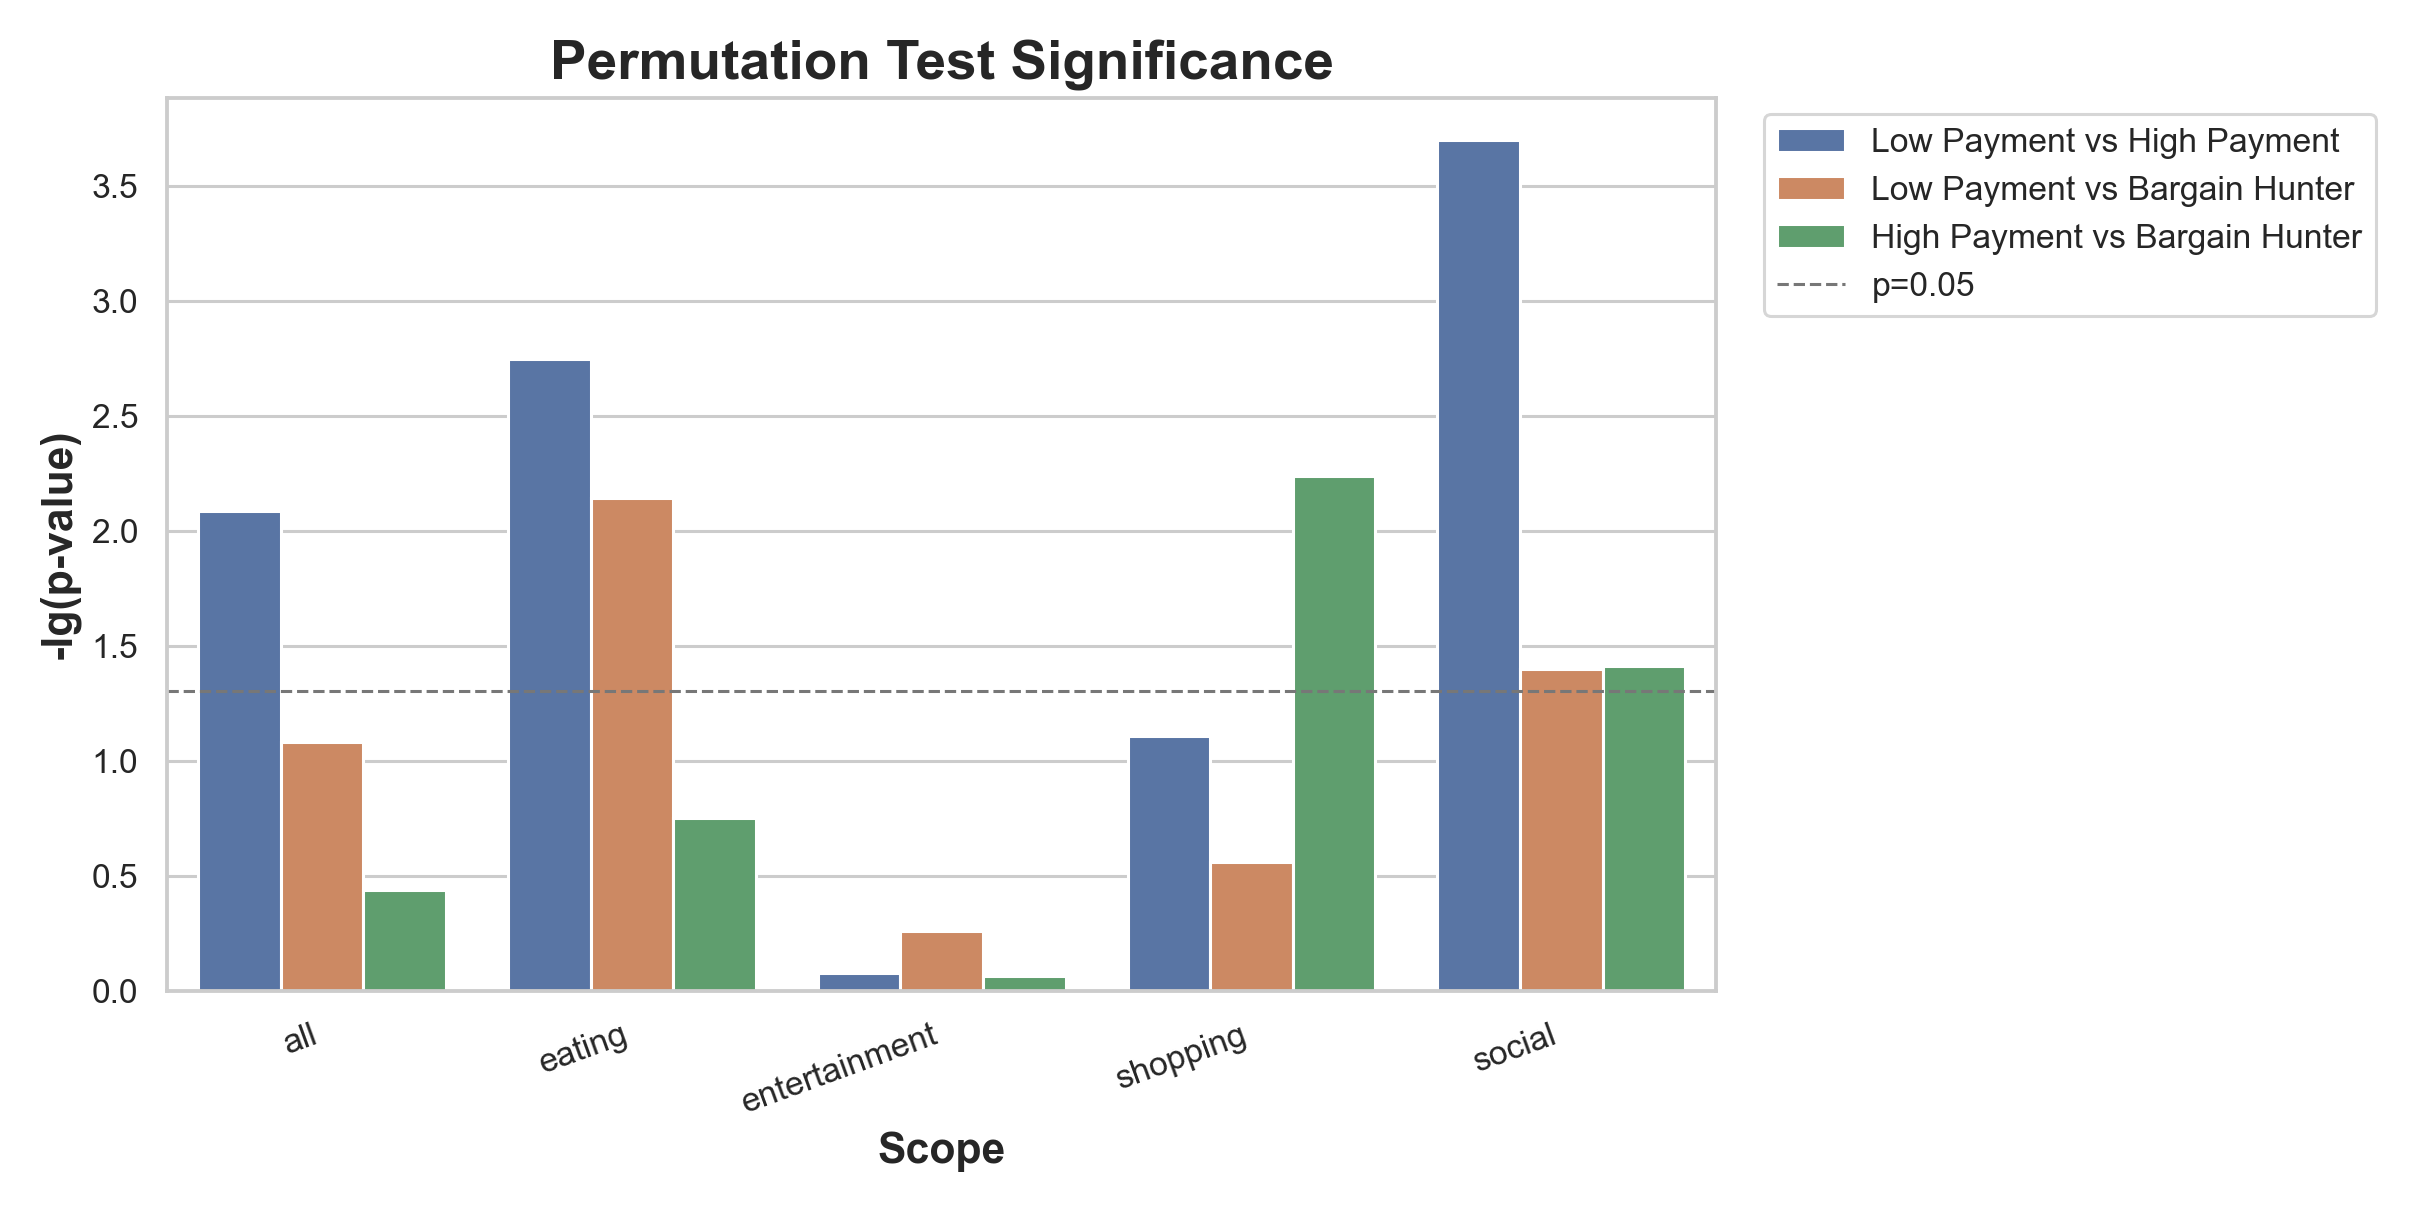
\includegraphics[width=0.95\linewidth]{figures/statistics/permutation_pvalues_by_scope.png}
    \caption{Permutation-test p-values by comparison scope based on binarized occurrence \(D_i>0\).}
    \label{fig:permutation-pvalues-appendix}
\end{figure}

\begin{figure}[htbp]
    \centering
    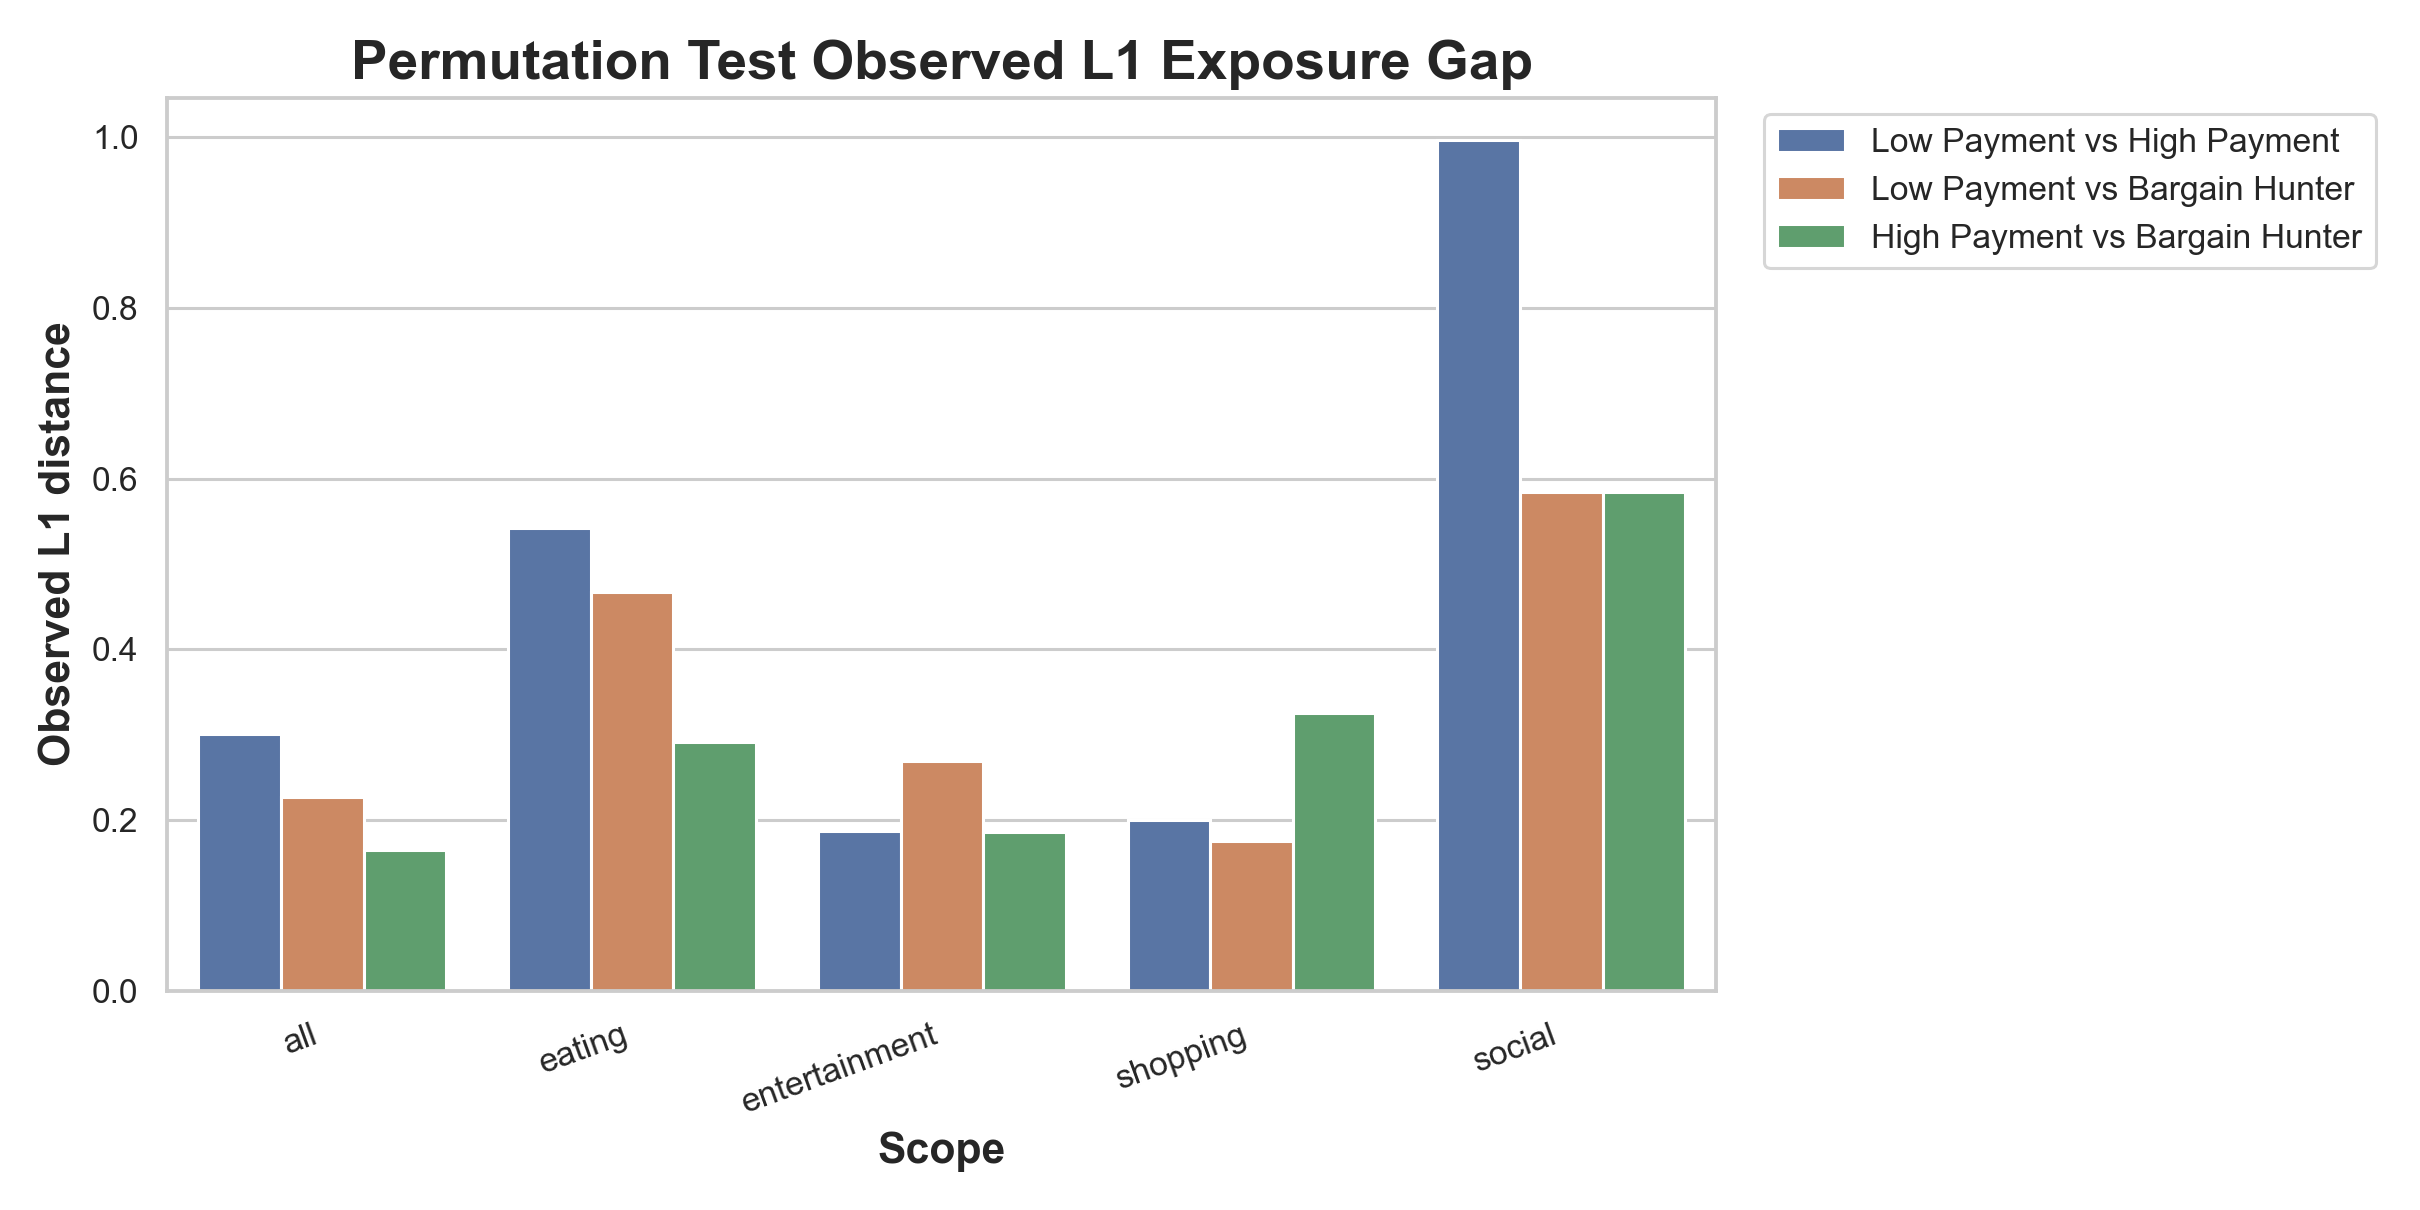
\includegraphics[width=0.95\linewidth]{figures/statistics/permutation_observed_l1_by_scope.png}
    \caption{Observed \(L_1\) exposure distances by comparison scope based on binarized occurrence \(D_i>0\).}
    \label{fig:permutation-l1-appendix}
\end{figure}

\begin{figure}[htbp]
    \centering
    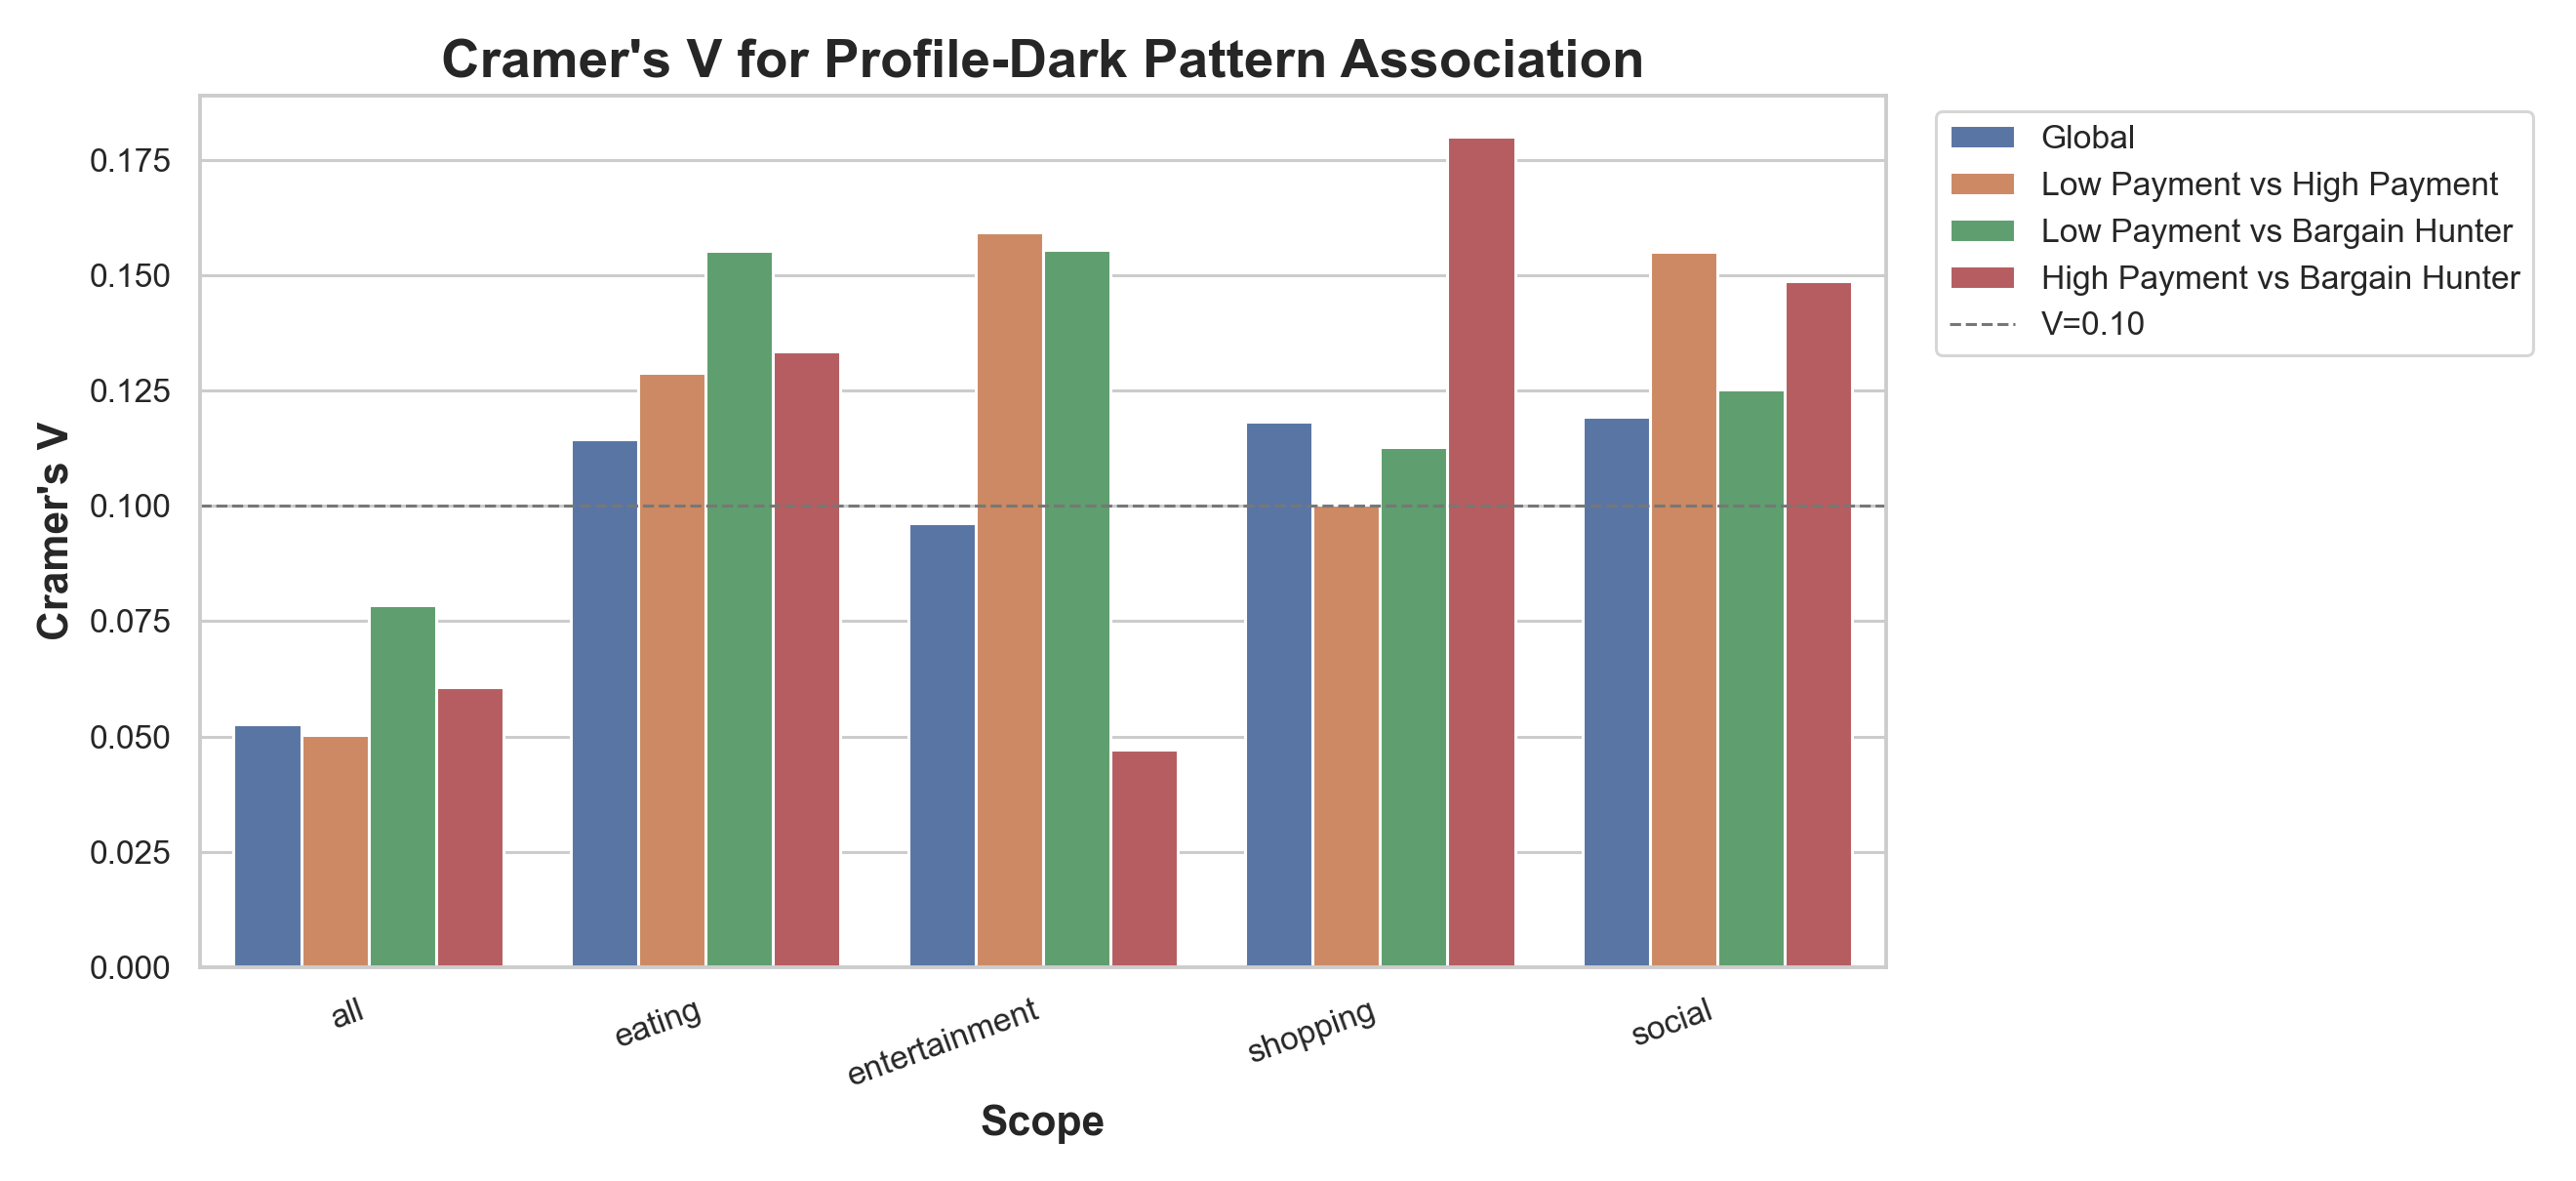
\includegraphics[width=0.95\linewidth]{figures/statistics/cramers_v_by_scope.png}
    \caption{Cramér's \(V\) association strength by comparison scope based on binarized occurrence \(D_i>0\).}
    \label{fig:cramers-v-appendix}
\end{figure}

The full convergence curves are interpreted as descriptive stability evidence rather than proof of causal convergence. If the running mean becomes less volatile after repeated interactions, this suggests that the target interaction budget is sufficient to produce a more stable estimate of profile-conditioned exposure within the archived trajectory. However, longer-term interaction histories may still reveal additional exposure dynamics.

\section{Appendix F: Statistical Validation Notes}
\label{app:statistical-validation-tables}

Appendix F documents how the statistical validation results are interpreted. The main report and Appendix~\ref{app:statistical-visualizations} report the exported plots for p-values, q-values, L1 distance, and Cramér's \(V\). These plots are read together rather than as independent proof from any single statistic.

The statistical validation is presented as evidence of association rather than causation. Since the experiment compares controlled profile-conditioned interaction traces, significant differences indicate that observed exposure patterns are unlikely to be explained solely by random profile assignment under the tested conditions. They are not interpreted as proving that the application intentionally targets a particular user group.

The permutation test summary describes how profile labels are randomly reassigned to construct a null distribution of exposure differences. The observed exposure gap is then compared against this null distribution. Low permutation p-values suggest that the observed gap is unusually large under random reassignment, while larger p-values suggest weaker evidence for a profile-associated difference.

In addition to statistical significance, the appendix reports practical difference measures. The \(L_1\) distance between two profile-level DPS exposure vectors is used to describe the magnitude of exposure difference:
\[
L_1(A_i, A_j) = \sum_{d \in DPS} 
\left| E(D_d \mid A_i) - E(D_d \mid A_j) \right|.
\]
Cramér's \(V\) can be used to summarize the strength of association between profile type and DPS exposure for categorical or discretized annotations. In this report, the contingency table is built from binarized DPS presence, so each dimension is first reduced to present versus absent before the counts are aggregated by profile. If future work adopts an ordinal 0/1/2 scheme, the positive levels should be collapsed into the presence category for this statistic or analyzed with a separate ordinal association measure. Reporting both significance and effect-size-oriented metrics helps avoid overinterpreting small but statistically detectable differences.

Together, these validation outputs provide empirical support for the report's main claim that dark pattern exposure can be estimated as a profile-conditioned outcome. The results should be discussed as observed differences under controlled audit conditions, rather than as direct evidence of intent or demographic discrimination.



\FloatBarrier

% =========================================================



\bibliographystyle{ieeetr}
\bibliography{refs}

\end{document}
